\documentclass[ITR,MA,english,final]{LSR_thesis} 
\graphicspath{{pics/}{logos/}}

\usepackage{psfrag,amsbsy,graphics,float}
\usepackage{graphicx, color} %deleted [dvips] in front of {graphicx, color} for usage with PDFLaTeX
%\usepackage[latin1]{inputenc}
%\usepackage{verbatim} 
\usepackage{amsmath,empheq}
\usepackage{amsfonts}
\usepackage{amssymb}
\usepackage[]{algorithm2e}
\usepackage{nomencl}
\usepackage{hyperref}
% \usepackage{natbib}
\newcommand\floor[1]{\lfloor#1\rfloor}
\newcommand\ceil[1]{\lceil#1\rceil}
\makenomenclature
\newcommand{\nm}[2]{\nomenclature{#1}{#2}}
\usepackage{tikz}
\usetikzlibrary{shapes.geometric,arrows}
\usetikzlibrary{intersections}

\usepackage{etex}
\reserveinserts{25}
\usepackage{morefloats}
\usepackage[section] {placeins}

\DeclareMathOperator*{\argmin}{\arg\!\min}



\tikzstyle{startstop}=[rectangle, rounded corners, minimum width=3cm, minimum height=1cm, text centered, draw=black, fill=red!30]
\tikzstyle{io}=[tropezium, tropezium left angle=70, tropezium right angle=110, minimum width=3cm, minimum height=1cm, text centered, draw=black, fill=blue!30]
\tikzstyle{io}=[tropezium, tropezium left angle=70, tropezium right angle=110, minimum width=3cm, minimum height=1cm, text centered, draw=black, fill=blue!30]
\tikzstyle{process}=[rectangle, minimum width=3cm, minimum height=1cm, text centered, draw=black, fill=green!30]
\tikzstyle{decision}=[diamond, minimum width=3cm, minimum height=1cm, text centered, draw=black, fill=green!30]

\usepackage{txfonts}
\renewcommand{\vec}[1]{\boldsymbol{#1}}
\setlength{\abovecaptionskip}{0pt}
\setlength{\belowcaptionskip}{10pt}
\usepackage{mathtools}
\newcommand\scalemath[2]{\scalebox{#1}{\mbox{\ensuremath{\displaystyle #2}}}}
\newtheorem{theorem}{Theorem}[chapter]
\newtheorem{corollary}{Corollary}[chapter]
\newtheorem{identity}{Identity}[chapter]
\newtheorem{lemma}[theorem]{Lemma}
%\theoremstyle{definition}
\newtheorem{definition}{Definition}[chapter]

%% Options:
%% LSR: LSR Template with Prof. Buss as default
%% ITR: ITR Template with Prof. Hirche as default

%% BA: Bachelorarbeit / Bachelor thesis
%% MA: Masterarbeit / Master thesis
%% HS: Hauptseminar / Scientific seminar
%% PP: Projektpraktikum / practical course
%% IP: Ingenieurpraxis
%% FP: Forschungspraxis
%% SeA: Semesterarbeit (MW)

%% english
%% german

%% final
%% intermediate

%%% last changes: 05.04.2016 (v.gabler@tum.de)

%_________MACROS_________ (optional and customizable - see output)
%% include packages for your work in here
\usepackage[colorinlistoftodos]{todonotes}        % for handling TODOs
\usepackage{setspace}
\usepackage{acronym}

% using the todonotes package in some nice ways (see packages.tex)
\newcommand{\add}[2][]{\todo[color=blue!40,#1]{#2}{}}
\newcommand\optional[2][]{\todo[inline, color=cyan!40, caption={2do},
	#1]{\begin{minipage}{\textwidth-4pt}#2\end{minipage}}{}}

% math macros
\newcommand{\set}[1]{\boldsymbol{#1}}
\renewcommand{\vec}[1]{\mathbf{#1}}


%_______Start_Document______________________________________
\begin{document}

%%%%%%%%%%%%%%%%%%%%%%%%%%%%%%%%%%%%%%%%%%%%%%%%%%%%%%%%%%%%%%%
%%%%%%%%%%%%%%%%%%% title page %%%%%%%%%%%%%%%%%%%%%%%%%%%%%%%%
%%%%%%%%%%%%%%%%%%%%%%%%%%%%%%%%%%%%%%%%%%%%%%%%%%%%%%%%%%%%%%%
%% for an english theis. The title:
\title{Trajectory-based Controller-Geometry-Codesign of Underwater Robots}
%% Für deutsche Arbeiten: Deutscher Titel:
% \title{Die Antwort auf Alles und Mehr - Ein Trauerspiel in 4 Akten}
% and English translation
%\titletranslation{Subtitle} 
% data about YOU!:
\student{Yongyu Chen} 			%% your name
\studtitle{B.Sc.} 			%% Bachelor of Arts, Dr.~phil, etc.
\street{Schr\"ofelhofstr. 22/0906}			%% your address
\city{81375 M\"unchen}								%		"
\phone{0176\,82559612}			%% your telephone-no.

%% if more students are involved (e.g. PP) 
%--the following parted is not tested ---
% please report bugs to v.gabler@tum.de 
%\studenttwo{Zweiter Student}
%\studtitletwo{} 
%\studentthree{} 
%\studtitlethree{} 
%\studentfour{} 
%\studtitlefour{} 
%-----------------------------------------
\supervisor{Dr.-Ing. Stefan Sosnowski}			%% your supervisor
\finalrep{27.10.2017}						%% final presentation / date

\maketitle
%%%%%%%%%%%%%%%%%%%%%%%%%%%%%%%%%%%%%%%%%%%%%%%%%%%%%%%%%%%%%%%
%%%%%%%%%%%%%%%%%%%%%%%%%%%%%%%%%%%%%%%%%%%%%%%%%%%%%%%%%%%%%%%

\newpage
\cleardoublepage
\phantom{u}
\phantom{1}\vspace{6cm}
\begin{center}
\add[inline]{In your final hardback copy, replace this page with the signed exercise sheet.}

\vspace{3cm}

\todo[inline,color=red!70]{Before modifying this document, READ THE INSTRUCTIONS AND GUIDELINES!}
\end{center}
\newpage

%%%%%%%%%%%%%%%%%%%%%%%%%%%%%%%%%%%%%%%%%%%%%%%%%%%%%%%%%%%%%%%
%%%%%%%%%%%%%%%%%%%%% abstract %%%%%%%%%%%%%%%%%%%%%%%%%%%%%%%%
%%%%%%%%%%%%%%%%%%%%%%%%%%%%%%%%%%%%%%%%%%%%%%%%%%%%%%%%%%%%%%%
\topmargin5mm
\textheight220mm
\pagenumbering{arabic}
\phantom{u}
\begin{abstract}
Conventionally, designing an underwater robot requires experienced experts
to adapt the robot structure to a series of designing requirements: buoyancy neutral, high surge velocity, low power consumption, low construction cost and small compact volume, etc. This is usually an iterative process, since most of the robot geometric variables are tightly coupled and immediately affect the vehicle dynamics and performance of the robot. Furthermore, due to the nonlinear and coupled nature of the robot dynamics, changes in the vehicle geometric variables strongly influence the control design. In this work, we propose a novel a system-engineering approach to the controller-geometry-codesign: kinematic and dynamic requirements are derived from a set of desired trajectories the robot should perform. Together with the conventional design requirements we formulate the robot designing procedure as multi-stage iterative optimizations.

Due to the customizable robot geometric structure, we build the robot in a modular way in this work. That is, the robot constituent parts are modeled as simple shapes parametrized by several geometric decision variables. The inertia matrices, Coriolis matrices, restoring matrix and the damping matrix can be calculated from them. As a result, a parametrized vehicle dynamic model indicating the intrinsic couplings among these decision variables is derived.

Trim trajectories are chosen in this thesis since along them the vehicle moves stably. It implies  that all velocities, roll and pitch angles as well as the hydrodynamic coefficients are constant. Based on these characteristics, we can linearize the dynamics of the error between the real robot' states and desired trim states uniquely. Each specified trim trajectory corresponds to a linear multi-input multi-output error dynamic system for a given robot geometry. Thus, the nonlinear robot dynamics is formulated as a linear switched system in the thesis and we utilize switched linear quadratic regulator to control the robot's moving trajectories.

Simulations for optimizing the actuator placements including six thrusters and four fins combined with two thrusters are performed, respectively. According to the simulation results, the proposed optimization algorithm is able to find a locally optimal and controllable robot geometry which can track the desired trim trajectories stably with a unconstrained switched LQR controller.


  
%\begin{center}	
%\normalsize \textbf{Zusammenfassung}\\
%\end{center}
%Hier die deutschsprachige Zusammenfassung. 
%\optional{Talk to your supervisor if this is needed and/or wanted before starting with your thesis}
\end{abstract}
\newpage

%%%%%%%%%%%%%%%%%%%%% Widmung %%%%%%%%%%%%%%%%%%%%%%%%%%%%%%%%%
\phantom{u}
\phantom{1}\vspace{6cm}
\begin{center}
%Hier die Widmung oder leer lassen
\end{center}


\pagestyle{fancy}

%%%%%%%%%%%%%%%%%%%Inhaltsverzeichnis%%%%%%%%%%%%%%%%%%%%%%%%%%
\tableofcontents 

%%%%%%%%%%%%%%%%%%%%%%%%%%%%%%%
% ACTUAL CONTENT OF YOUR WORK %
%%%%%%%%%%%%%%%%%%%%%%%%%%%%%%%
%%%%%%%%%%%% Kapitel - externe Dateien zur Ordnung%%%%%%%%%%%%%
\chapter{Introduction and Related Work}
\section{Introduction}
%\cite{Kato1998,Prasad2013,Lindegaard2003,Ridley2003,Perez2002,JUNKINS1991}
Two-thirds of the earth is covered by the ocean and the underwater robots can help us to explore and perform various tasks in this hazardous and uneasily attainable environment. The autonomous underwater vehicles (AUVs) have various application areas. For scientific purpose, they can be used for seafloor mapping or geological sampling. In the environmental area, people utilize them to inspect the underwater structures like pipelines, dams, etc. or to monitor the pollution. Besides, underwater robots also bring convenience to the ocean survey and undersea structures' construction and maintenance~\cite{Yuh2000}. 

A good manoeuvring performance of underwater robots requires an appropriate robot structure adapting to the specific mission. This is a tough and time-consuming task involving many iterations of design and testing, even though for skilled expert. A simple underwater robot prototype includes CPU, the inertial navigation system, the sensory and communication system, and the power supply system (batteries). All of them are enclosed in a protecting hull. Besides, thruster and control fins are the main actuators. Their properties, numbers and locations will influence the robot's working performance heavily. Hence, a good designer should be able to find a suitable configuration of these components.

Traditionally, after the robot was built by the designer, the users will analyse the dynamics based on the current robot structure and actuator configuration. Then they will plan the trajectory and design the controller based on this dynamic model and the task requirements. 

In this work, we separate the hull design and the actuator placement optimization. Designing the hull should satisfy the conventional specifications: buoyancy neutral, maximal surge velocity, maximal working time and low construction cost and a minimal volume to contain the inertial measurement unit, CPU and communication system. In terms of the actuator design we start from an innovative designing direction. That is, a set of requirements for kinematics and dynamics is directly derived from a set of trajectories the vehicle should perform. A suitable trajectory representation should be chosen and key requirements should be identified. In the design phase, an automated co-design of the optimal kinematics and dynamics of the robot together with the synthesis of a stable controller for tracking is aimed for. 

In Chapter 2, we propose a modular modeling method for the underwater robot prototype. Each component can be modeled as sample geometric shape determined by several geometric variables and then we can parametrize the robot dynamics with these variables. 

From deep-sea exploration to underwater rescue, underwater vehicles require efficient path planning algorithms. An relative simple but representative trajectory is expected for designing the robot. So we use the trim trajectory since robot's motion is stable along them. Partial kinematic states ($\phi$, $\theta$), the dynamic states (linear and angular velocities) that influence the robot dynamics and therefore the hydrodynamic coefficients depending on velocities stay constant along the trim trajectory. A set of desired trim trajectories give us firstly information about the desired position for the robots. By adopting the Frenet-Serret frame, the desired orientation and the desired velocity along the trajectory will be derived in further. With the full information about the system states, we are able to formulate the error dynamics. These will be introduced in Chapter 3. 

For analysis and controller design of nonlinear systems the typical approach is to linearize the nonlinear system. In this work we adopt a trajectory-based linearization way for the error dynamics usd in~\cite{Silvestre2002} for the following reasons. Firstly, for a specific trim trajectory segment the linearized error dynamics is unique. Hence, we can implement a number of analysing approaches for linear systems for the error dynamics. Secondly, tracking a desired trajectory is a concern for practical manoeuvring tasks. The error dynamic formulation along trim trajectories will be illustrated in Chapter 4. Moreover, task-specific trajectories for underwater robots can be planned as a combination of a set of trim trajectories, which means that we also have a set of linearized MIMO error dynamics. Thus, we design a switched LQR controller based on these linear systems. This will also be discussed in the same chapter.    

The main contribution of this work is to find an optimal geometric configuration of the robot constituent parts. Based on the parametrized underwater vehicle model built in Chapter 2, we are able to identify the relationship between the geometric decision variables and each term in the dynamic model (the mass matrix, the Coriolis matrix, the damping matrix and the restoring matrix). After that, we propose two optimization algorithms which find a locally optimal hull size and a local optimum for actuator placement, respectively.

In Chapter 6, we utilize the geometry from the optimization results and calculate the corresponding optimal dynamics. Regular underwater robots are normally equipped with actuators symmetrically in pairs. These new built robots are visualized to provide us a more intuitive impression about the irregular robots. The irregularity      is caused by the randomly generated initial geometric decision variables and the nonlinear optimization algorithm that is only able to find a local minimum depending on the initial values. The controllability of the current designed robot system is verified by means of checking the tracking performance along a set of trim trajectories. 

Underwater dynamics are nonlinear, highly coupled, MIMO systems with six degrees of freedom (DOFs). When we change
the geometric parameters of hull and actuators or the number of actuators, the geometric center, the center of buoyancy, the inertia matrix, the Coriolis matrix and the hydrodynamic damping will also change consequently. In addition, the modeling of thrusters and control fins is not accurate enough to indicate their real physical characteristics. To make the optimization solvable, we make a list of assumptions. These inaccuracies can be rectified and the optimization performance can be enhanced for future works. These limitations and the possible improvements will be discussed in the last chapter. 

The complete underwater robot designing and verification processes proposed in this thesis are concluded in Figures~\ref{FIG:DesignPhase} and~\ref{FIG:VerificationPhase}. 
\begin{figure}
\centering
\includegraphics[width=0.95\textwidth]{DesignPhase.eps}
\caption{Underwater robot geometric design procedure}	
\label{FIG:DesignPhase}
\end{figure}
\begin{figure}
\centering
\includegraphics[width=0.7\textwidth]{VerificationPhase.eps}
\caption{Verification of geometric design}	
\label{FIG:VerificationPhase}
\end{figure}
\section{Related Work}
Our work draws from a number of ideas and methods from underwater robot modelling, error dynamics and controller design and computational robot design.
\subsection{Underwater Robot Modular Dynamic Modeling}
The chapter 7 of~\cite{F2011} introduces 1 DOF heading autopilot model, 3DOF manoeuvring and dynamic positioning (DP) models, 4 DOF manoeuvring and 6 DOF coupled system for advanced 6DOF manoeuvring model. Especially for underwater robots with actuation in all DOFs, a nonlinear, strongly coupled, MIMO dynamic 6DOF model is required for the model-based controller and observer design. The detailed derivation can be found in the appendix \ref{Appendix:DM} summarized from~\cite{F2011,F1994,FF1995,AG2014}.

Our goal is to design algorithms finding an optimal configuration for AUVs. It requires the robots to have a flexible modularized structure so that we can reconfigure the robot prototype easily.  In~\cite{Vasilescu2005}, a novel modular  underwater robot which can self-reconfigure by stacking and unstacking its component modules is designed. A modular dynamic modeling is desired for this flexible robot structure. With help of this method, the dynamic equation can be parametrized with geometric variables (location, size etc.) and especially the hydrodynamic coefficients can be estimated from them. The modular modeling methods are discussed in~\cite{Chen2007} and~\cite{Sia1999}.
\subsection{Controller Design and Path Planning}
Due to the requirement of full-DOF control, underwater robot control is a very challenge task. Diverse control methods can be implemented for the robot, e.g., adaptive control (\cite{JYuh1990,Svein1991}), sliding model control (\cite{JSoltine1985,Narimani2006}), feedback linearization (\cite{Wadoo2003}), backstepping (\cite{Jian2015,Wadoo2003}).

In~\cite{Makdah2016}, the 6 degrees of freedom (6DOF) dynamics and kinematics model of the underwater robots is linearized about the given desired trajectory. A linear time variant (LTV) state space model for underwater robots is obtained. And then a linear quadratic controller is designed according the linear models and applied to the nonlinear robot dynamics to track the desired trajectory. Our idea is very similar to this, we also want to linearize the nonlinear model along the trajectory. However, since we should utilize the linear models for the following optimization algorithm, a relative small number of linearized models is expected for the given trajectory. By special nonlinear transformation~\cite{RNC705} along trim trajectory, the error dynamics between the real robot states and the trajectory-determined states can be uniquely linearized, which satisfies our trajectory design aim. The trim trajectory is widely used for unmanned aerial vehicles (UAVs) because of its simplicity for controling and analysing. Its benefits and practical usages can be found in~\cite{Beji2005,Bottasso2008,Sebbane2015}.
   
\subsection{Computational Design}
The basic idea of this work was inspired from~\cite{Du2016}. In this paper, Du et al. proposed  an  interactive  procedure to computationally design, optimize, and fabricate multicopters. The multicopter can be constructed from  a  collection  of  components including propellers, motors, and carbon fiber rods. They proposed an algorithm optimizing shape and controller parameters of the current design to ensure the multicopter's proper operation. Other merics including payload, battery usage, size, and cost are integrated into the optimization algorithm.

Generally speaking, both underwater robot and multicopter has the 6DOF dynamics. In spite of this, the underwater robots usually have full 6DOF actuation and thus contain a number of equilibrium points, while the multicopter stays at the equilibrium when the total resultant thrust equal to the gravity and the total result moment is equal to zero. In addition, beside the thrusters the underwater robots have also fins as control surfaces and their hydrodynamic characteristics are nonlinear and of high-order. The underwater robots possess a more complicated structure, making the geometric optimization a challenging task.

There are still a lot other works concerning the computational design of robots. In~\cite{Schulz2014}, a data-driven method for designing 3D models that can be fabricated was proposed. Schulz et al. propose the end-to-end system for design of robots with ground locomotion~\cite{Schulz2017}. The biggest advantage of the computational design is that it allows people of all skill level to design and fabricate robots.   

\subsection{Geometric Optimization}
\cite{JOUNG201244} present a methodology to optimize the AUV profile in order to reduce the total resistance with Computational Fluid Dynamics (CFD). The majority of works in terms of actuator optimization discusses the control allocation problem, e.g \cite{Fossen2008,Johansen2004,Johansen2005}.

In~\cite{XU20151044}, Xu et al. propose a novel local optimization of thruster configuration based on a synthesized  positioning  capability  criterion.

In our work, we optimize not only the hull but also the actuator configuration and our actuator includes thrusters and control fins. The control location problem normally formulated as optimization problems whose objective is to produce the specified generalized forces to minimize the control effort (power consumption), the position of thrusters is already fixed after the robot design is finished. In this case, the decision variables are normally the azimuth angle of the thrusters and the forces generated by them. Our optimizations are performed during the design phase. Hence, our decision variables contain not only the thrust forces, more importantly, an optimal thruster location should be found. Similarly, the deflection angle and the fin location should be optimized at the same time. 

\section{Contributions}
To summarize, our main contribution in this work include:
\begin{itemize}
\item Deriving the design requirements for robot kinematics and dynamics from a set of trim trajectories.
%\item Identifying important geometric variables determining the underwater robot dynamics. Define  are identified and the underwater robot dynamics is parametrized by these parameters; 
\item Approximating each constituent module of the underwater robot as a simple shape determined by several geometric decision variables and building the robot dynamics parametrized with them.
\item Identifying the couplings among all geometric decision variables.
\item Formulating an optimization problem that can optimize the size of the robot hull enclosure according to different design specifications.
\item Formulating an optimization problem that can jointly optimize positions and orientations, spin directions and control parameters satisfying the trajectory-based design requirements. 
\item Linearizing and transforming the nonlinear underwater robot dynamic system into a linear switched system, designing the switched Linear Quadratic Regulator (LQR) for the system.
\item Finding the state cost matrices and the input cost matrices for the switched  
LQR based on the stability.
\item Providing an efficient numerical approach to solve the actuator placement optimization by using the multi-stage iterative optimization method.
%\item  Providing an efficient numerical method to solve the underwater robot optimization problem and show its efficacy by optimizing different types of non-standard underwater robots
\end{itemize}








%_________Einleitung__________________________________
\chapter{Modular Modeling of Underwater Robot Prototype}

Based \cite{opencv_library} on the ideas of the computational underwater robot design, the designer should be able to assemble a underwater robot from a collection of components (hull enclosure, batteries, fins, thrusters, CPU, IMU, sensor and so on). The customizable robot structure implies the robot dynamics is determined by number and type of constituent components and their geometric variables. Unlike the conventional modeling method for which all components are fixed, in this chapter, we model the robot modularly. More precisely, each robot component is approximated as simple geometric shape determined by several size parameters. Then we can parametrize the mass, the moment of inertia and the hydrodynamic coefficients with these parameters. In addition, the position and orientation parameters also contribute the dynamics of the whole robot. By means of this modeling approach, a customizable dynamic model is obtained.

The underwater vehicles are mainly composed of hull and actuators and actuators can be further divided into thrusters and control fins. The modular modeling method is mainly adapted from~\cite{Sia1999}. We only consider the hydrodynamic effects of hull, while the added mass and hydrodynamic damping of fins and thrusters are also calculated. Also, we ignore the moment of inertia of fins and thrusters and assume that it is merely determined by hull components. Besides, we take the electronic devices into account and model them as cuboid. They have contribution to the total mass and moment of inertia of the robot and specify the minimal size of the hull volume.   

The inertia tensor for each modular component $s$ with respect to its center of mass $CG_{s}$  is given by
\begin{align}
\emph{\textbf{I}}_{g,s}=
\begin{pmatrix}
I_{xx,s}&0&0\\
0&I_{yy,s}&0\\
0&0&I_{zz,s}
\end{pmatrix}.
\end{align} 

\section{Modeling of Hull Components}
As the main body of the underwater robot, the navigation system, sensory system and the power supply system are embedded in it. 

The hull shell is modeled as hollow cylinder, as illustrated in Figure ~\ref{fig:HullModeling}. We use three parameters to characterize it including the inner radius $r_{H,i}$, the outer radius $r_{H,o}$ and the hull length $l_{H}$. Then its mass and moment of inertia with respect to its center of gravity can be calculated as follows:   
\begin{figure}
\centering
\begin{tikzpicture}[x=1.5cm,y=1.5cm,>=latex']
	\coordinate (O) at (0,0) node[above] {\small ${CO}$};
	\draw[black,fill=black] (0,0) circle (.5ex);
	\draw (-1.55,-1.515) arc (-30:30:0.5);
	\draw (-1.55,-1.515) arc (-150:-210:0.5);
	\draw (-1.55,-1.515) arc (75:15:0.5);
	\draw (-1.55,-1.515) arc (195:255:0.5);
	\draw (-1.55,-1.515) arc (-15:-75:0.5);
	\draw (-1.55,-1.515) arc (105:165:0.5);
	\draw [->,blue,line width=0.65mm,] (-1.5,-1.5) (O) -- (-1.55,-1.515)node[midway,above] {\small $\vec{r}_{T}$};
    \draw [->,blue,line width=0.65mm,] (-2,-2) arc[x radius=0.75cm, y radius =.75cm, start angle=-150, end angle=-30]node[below right] {\small $\vec{b}_{T}$};
	\draw[black,fill=black] (-1.55,-1.55) circle (.4ex);
	\draw [->,blue,line width=0.65mm,](-1.55,-1.515) -- (-1,-1.55) node[right] {\small $\vec{d}_{T}$};
	\coordinate (OD) at(0,-1);
	% plot the x-axis
	\draw [dashed] (O) -- (2,0);
	\draw [dashed] (O) -- (0,-1);
	\draw [->](2,0) -- (3,0) node[right] {$x_{b}$};
	\draw [dashed] (O) -- (-2,0);
	\draw [->](0,-1) -- (0,-2) node[below right] {$z_{b}$};
	\draw (-2,0) circle(0.3 and 1);
	\draw (-2,0) circle(0.24 and 0.8);
	\draw [dashed](2,0) circle(0.24 and 0.8);
	\draw [dashed](0,0) circle(0.24 and 0.8);
	\draw [dashed] (2,1) arc[start angle=90,end angle=270,x radius=0.3,y radius=1];
	\draw [name path=P2] (2,1) arc[start angle=90,end angle=-90,x radius=0.3,y radius=1];
	\draw [dashed] (0,1) arc[start angle=90,end angle=270,x radius=0.3,y radius=1];
	\draw [name path=P] (0,1) arc[start angle=90,end angle=-90,x radius=0.3,y radius=1];
	\draw (-2,1)--(2,1);
	\draw (-2,-1)--(2,-1);
	\path [name path=PP] (O) -- (1,-1);
	\path [name intersections={of=P and PP}];
	\coordinate (X1) at (intersection-1);
	\draw[dashed] (O)--(X1);
	\draw [->](X1) -- (1.35,-1.35) node[below left] {$y_{b}$};
	\draw [<->] (-2,1.2) -- (2,1.2) node [midway, above] {$l_{H}$};
	\draw (-2,1.1)--(-2,1.4);
	\draw (2,1.1)--(2,1.4);
	% legend for the radius
	\draw (-2.1,1)--(-3.5,1);
	\draw (-2.1,0)--(-3.5,0);
	\draw (-2.1,0.8)--(-2.9,0.8);
    \draw [<->] (-3,0) -- (-3,1) node [midway, left] {$r_{H,o}$};
    \draw [<->] (-2.5,0) -- (-2.5,0.8) node [midway, left] {$r_{H,i}$};
	\end{tikzpicture}
\caption{Modeling of hull as hollow cylinder} \label{fig:HullModeling}
\end{figure}
\begin{align}
m_{H}=\rho_{H}\pi (r_{H,o}^{2}-r_{H,i}^{2})l_{H},
\end{align}
\begin{align}
I_{xx,H}=\dfrac{1}{2}m_{H}(r_{H,o}^{2}+r_{H,i}^{2}),
\end{align}
and
\begin{align}
I_{yy,H}=I_{zz,H}=\dfrac{1}{4}m_{H}(r_{H,o}^{2}+r_{H,i}^{2}+\dfrac{l_{H}^{2}}{3}).
\end{align}
In the following part, we simplify the notation of $r_{H,o}$ as $r_{H}$.
Within the hull, we model the battery as solid cylinder, based on the defined coordinate in \ref{fig:BatteryModeling}, the mass and moment of inertia are given as
\begin{align}
m_{bat}=\rho\pi r_{bat}^{2} l_{bat},
\end{align}
\begin{align}
I_{xx,bat}=I_{yy,bat}=\dfrac{1}{12}m_{bat}(3r_{bat}^{2}+l_{bat}^{2}),
\end{align}
and
\begin{align}
I_{zz,bat}=\dfrac{1}{2}m_{bat}r_{bat}^{2}
\end{align}
\begin{figure}
\centering
\begin{tikzpicture}[x=1.5cm,y=1.5cm,>=latex']
	\coordinate (O) at (0,0);
	\coordinate (OD) at(0,-1);
	\draw[dashed] (O) -- (1,0);
	\draw [->](1,0) -- (2,0) node[right] {$x$};
	\draw[dashed,-serif cm] (O) -- (0,-1);
	\draw[dashed,-serif cm] (O) -- (0,1);
	\draw [->](0,-1) -- (0,-2) node[below right] {$z$};
	\draw (0,1) circle(1 and 0.3);
	% \draw (0,-1) circle(1 and 0.3);
	\draw[dashed] (O) +(0:1) arc[start angle=0,end angle=180,x radius=1,y radius=0.3];
	\draw[name path=P] (O) +(0:1) arc[start angle=0,end angle=-180,x radius=1,y radius=0.3];
		\draw[dashed] (OD) +(0:1) arc[start angle=0,end angle=180,x radius=1,y radius=0.3];
	\draw[name path=PD] (OD) +(0:1) arc[start angle=0,end angle=-180,x radius=1,y radius=0.3];
	\draw (-1,-1)--(-1,1);
	\draw (1,-1)--(1,1);
	\path[name path=P1] (O) -- (-1,-1);
	\path [name intersections={of=P and P1}];
	\coordinate (X1) at (intersection-1);
	\draw[dashed] (O)--(X1);
	\draw [->](X1) -- (-1.35,-1.35) node[below left] {$y$};
	\draw [<->] (-1.2,1) -- (-1.2,-1) node [midway, left] {$l_{bat}$};
	\draw (-1,1.1)--(-1,1.4);
	\draw (0,1)--(0,1.4);
    \draw [<->] (-1,1.2) -- (0,1.2) node [midway, below] {$r_{bat}$};
    	\end{tikzpicture}
\caption{Modeling of battery as solid cylinder} \label{fig:BatteryModeling}
\end{figure}
All other devices are assumed to have a constant mass $m_{d}$ and a constant moment of inertia $\emph{\textbf{I}}_{d}$ with respect to the body frame.

\section{Modeling of Control Actuators}
Usually, fins and thrusters are used as actuators. In the second optimization phase, we want to optimize the geometric parameters of all actuators. For the design of robots, geometric placement of all  actuators plays an decisive role for controlling performance. To find an optimal geometric properties of actuators in the designing phase, appropriate models for actuators are required to estimate the generated control efforts under different actuator configurations, and the lift of fin is treated as the control input.  
 
\subsection{Modeling of Thrusters}
\label{Subsection:ModelingofThrusters}
For modeling of thrusters, we adopt the modeling methods from~\cite{Du2016}. 
Based on this modeling, each thruster is parameterized by the motor orientaion $\vec{d}_{T}$~(unit vector), the motor position $\vec{r}_{T}$ in the body frame $\lbrace b \rbrace$ and the motor spin direction  $b_{T}\in \lbrace-1,1\rbrace$. We use $u_{T}$ and $m_{T,r}$ to denote the magnitude of the thrust force and torque generated by the propeller rotation, respectively.

Yoerger et al.~(\cite{PropellerModel}) proposed the one-state model for the propeller.
The torque $Q_{m}$ and thrust $T$ has the following relationship:
\begin{align}
\dot{\omega}_{p}=\beta Q_{m}-\alpha\omega_{p}|\omega_{p}|
\label{EQ:PropellerDynamics1}
\end{align}
\begin{align}
T=C_{t}\omega_{p}|\omega_{p}|
\label{EQ:PropellerDynamics2}
\end{align}
where $\omega_{p}$ is the propeller angular velocity, $\alpha$ and $\beta$ are constant model parameters and $C_{t}$ is a proportionality constant. The three parameters $\alpha$, $\beta$ and $C_{t}$ require to be identified. 

%Within each trim trajectory segment, all desired inputs should be constant, thus %the spinning velocity should be time-invariant, 
%i.e. $\dot{\omega}_{p}=0$, 
If the propeller rotates at steady state, i.e. $\dot{\omega}_{p}=0$, then according to (\ref{EQ:PropellerDynamics1}) and (\ref{EQ:PropellerDynamics2}), the relationship between the thrust generated by the propeller and the rotation torque can be described with the following equation:
\begin{align}
Q_{m}=\dfrac{\alpha}{C_{t}\beta}T,
\end{align}
which means that the torque generated due to the rotation of propellers is proportional to the thrust force of the propeller. Thus, we can assume the torque $m_{T,r}$ is proportional to the thrust force $u_{T}$
\begin{align}
m_{T,r}=\lambda_{T} u_{T},
\end{align}   
where $\lambda_{T}$ is the torque-force ratio. Taking the thruster motor orientation and the spin direction into consideration, we can have the rotation torque vector as
\begin{align}
\vec{m}_{T,r}=b_{T}\lambda_{T} u_{T}\vec{d}_{T}.
\end{align} 
Additionally, the thrust force will produce the thrust torque $\vec{m}_{T,t}$. For calculation of thrust torque, the center of gravity is assumed to be located in the body frame origin $CO$. Then the thrust torque can be expressed as
\begin{align}
\vec{m}_{T,t}=\vec{r}_{T}\times u_{T}\vec{d}_{T},
\end{align}
where $\vec{r}_{T}=(x_{T}, y_{T}, z_{T})$ is the position vector of the thruster in the body frame $\lbrace b \rbrace$.
Combining the thrust torque and the rotation torque, we express the total torque produced by a thruster as 
\begin{align}
\vec{m}_{T}=\vec{m}_{T,r}+\vec{m}_{T,t}=b_{T}\lambda_{T} u_{T}\vec{d}_{T}+\vec{r}_{T}\times u_{T}\vec{d}_{T} \in \mathbb{R}^{3}
\end{align}

The force direction is determined by the thruster motor orientation $\vec{d}_{T}$ and the force vector $\vec{f}_{T}$ can be represented as
\begin{align}
\vec{f}_{T}=u_{T}\vec{d}_{T} \in \mathbb{R}^{3}
\end{align}
The generalised force vector for thruster is defined as
\begin{align}
\vec{\tau}_{T}=\begin{pmatrix}
\vec{f}_{T} \\ \vec{m}_{T}
\end{pmatrix}
\end{align} 
If we treat the thrust as the control input, we can define an unique mapping vector for a thruster based on its geometric parameters.
\begin{align}
\emph{\textbf{B}}_{T}=
\begin{pmatrix}
\vec{d}_{T} \\
b_{T}\lambda_{T} \vec{d}_{T}+\vec{r}_{T}\times \vec{d}_{T}
\end{pmatrix} \in \mathbb{R}^{6}. \label{EQ:ThrusterMappingVector}
\end{align}
Then the generalised force generated by thrust can be in the following form:
\begin{align}
\vec{\tau}_{T}=\emph{\textbf{B}}_{T}u_{T}
\end{align}
 
\subsection{Modeling of Control Fins}
An accurate hydrodynamic modeling of control fins in Appendix C introduces high order nonlinear terms into the input matrix $\emph{\textbf{B}}_{a}$. The velocity of fin middle point in the body frame $\lbrace b \rbrace$ is denoted by $\vec{v}_{fin}=(u_{fin},~v_{fin},~w_{fin})^{T}$ and its three components have the following relationship with the robot linear velocity $\vec{v}=(u,~v,~w)^{T}$: 
\begin{align}
u_{fin}=u+z_{fin}q-y_{fin}r,
\end{align}
\begin{align}
v_{fin}=v+x_{fin}r-z_{fin}p,
\end{align}
\begin{align}
w_{fin}=w+y_{fin}p-x_{fin}q.
\end{align}
Then the fin velocity $\vec{v}_{fin}^{f}=(u_{fin}^{f},~v_{fin}^{f},~w_{fin}^{f})^{T}$ in the fin frame $\lbrace f \rbrace$ is calculated as:
\begin{align}
\vec{v}_{fin}^{f}=\emph{\textbf{R}}_{b}^{f}\vec{v}_{fin},
\end{align}
where $\emph{\textbf{R}}_{b}^{f}$ is determined by the fin position vector $\vec{r}_{F}$ in the body frame $\lbrace f \rbrace$. Then the angle of attack $\alpha$ is calculated as
\begin{align}
\alpha=atan2(w_{fin}^{f},u_{fin}^{f}).
\end{align} 
The $atan2$ can not be approximated by a polynomial term numerically. Furthermore, the lift and drag coefficients $C_{L}$, $C_{D}$ are piecewise functions of the angle of attack $\alpha$. We are able to use high-order polynomials to approximate them. The lift coefficient characteristic curve is depicted in Figure~\ref{FIG:LiftCoefficient}. The curve fitting result is shown in Figure~\ref{FIG:LiftApprox} and the relationship between $C_{L}$ and the attack angle $\alpha$ is
\begin{align}
C_{L}=-0.1463\alpha^{8}+1.234\alpha^{6}-3.61\alpha^{2}+0.09403.
\end{align}
Similarly, we are able to approximate the drag coefficient characteristic curve in~\ref{FIG:DragCoefficient} with high-order polynomials whose result is depicted in Figure~\ref{FIG:DragApprox}. The fitting function is:
\begin{align}
C_{D}=-0.4653\alpha^{9}-3.219\alpha^{7}+8.356\alpha^{5}-9.75\alpha^{3}+3.729\alpha.
\end{align}
These two high-order terms require considerably large computational capacity for the optimization. The aforementioned two problems from accurate hydrodynamic modeling make the optimization problem nearly unsolvable.

\begin{figure}
\centering
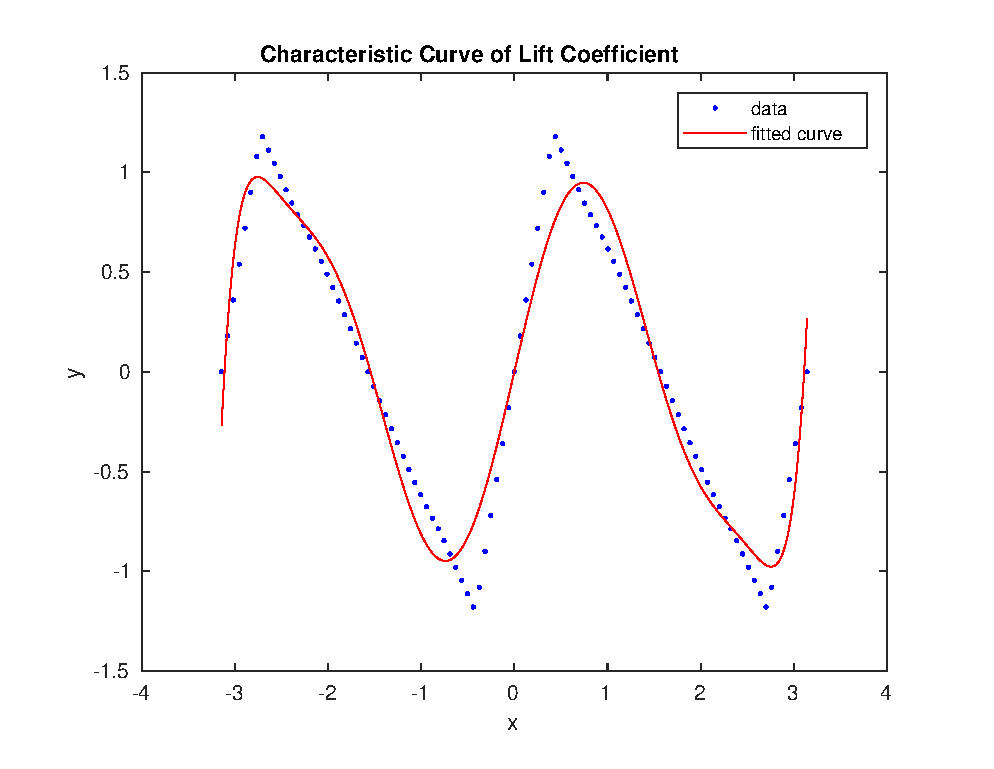
\includegraphics[width=0.75\textwidth]{liftappro.eps}
\caption{Approximation of relationship between lift coefficient $C_{L}$ and attack angle $\alpha$}	
\label{FIG:LiftApprox}
\end{figure}
\begin{figure}
\centering
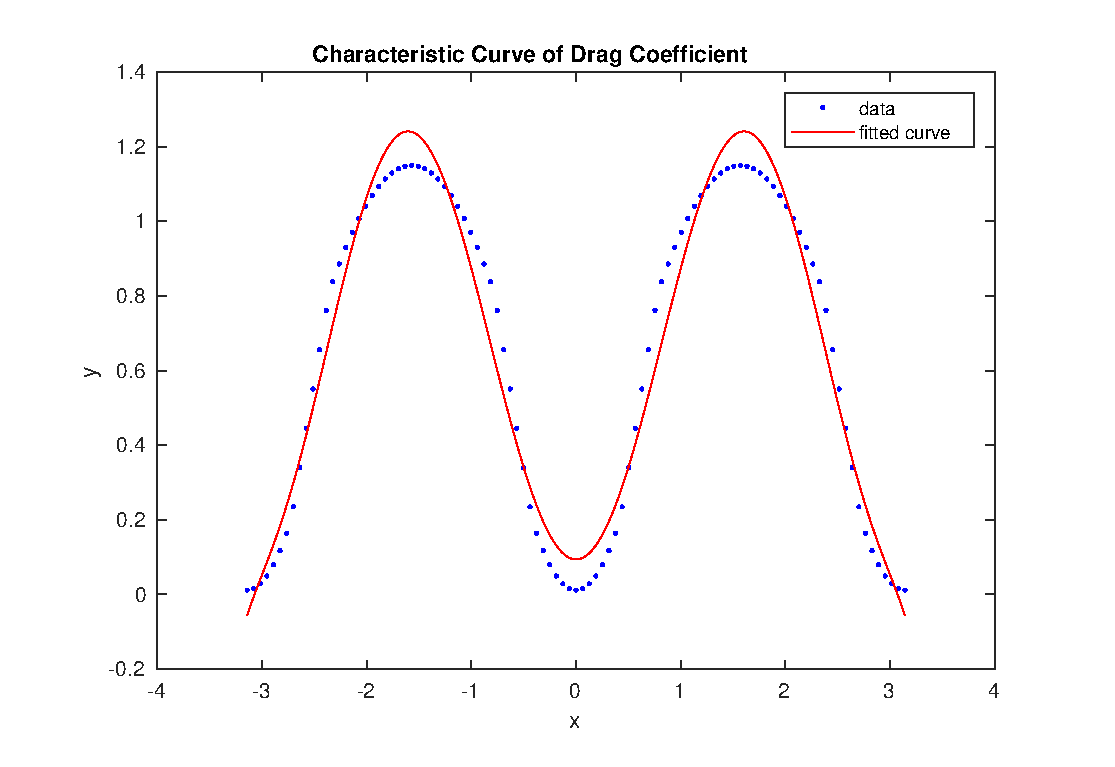
\includegraphics[width=0.75\textwidth]{dragappro.eps}
\caption{Approximation of relationship between drag coefficient $C_{D}$ and attack angle $\alpha$}	
\label{FIG:DragApprox}
\end{figure}
Strict restrictions on the fin geometric property, for instance the fins can only be mounted on the horizontal and vertical planes of the hull or they must be placed symmetrically in pairs , will bring the robot design back into the traditional way. 

A compromise can be found by means of small angle of attack assumption which is inspired by modeling methods in~\cite{FinModeling}.
\begin{figure}
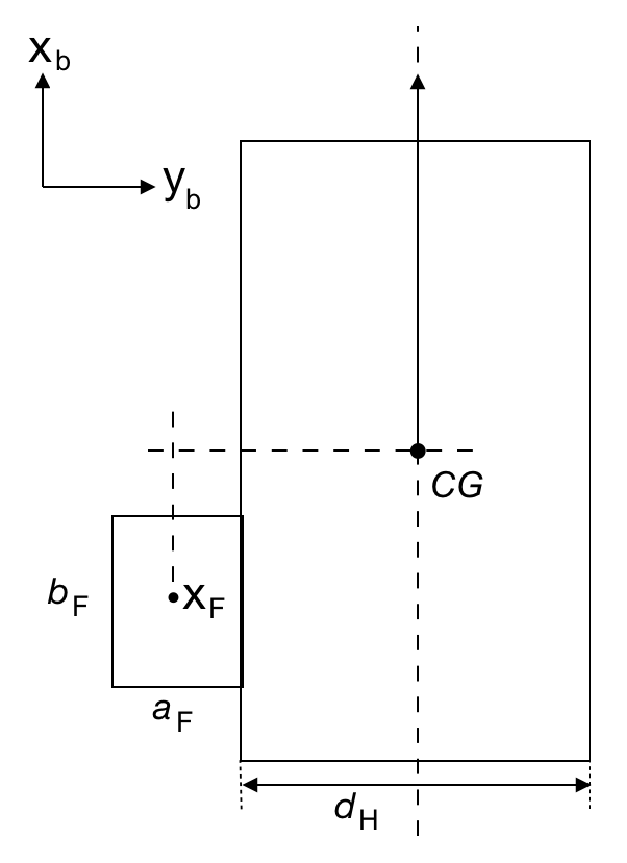
\includegraphics[width=0.4\textwidth]{FinLocation1.eps}
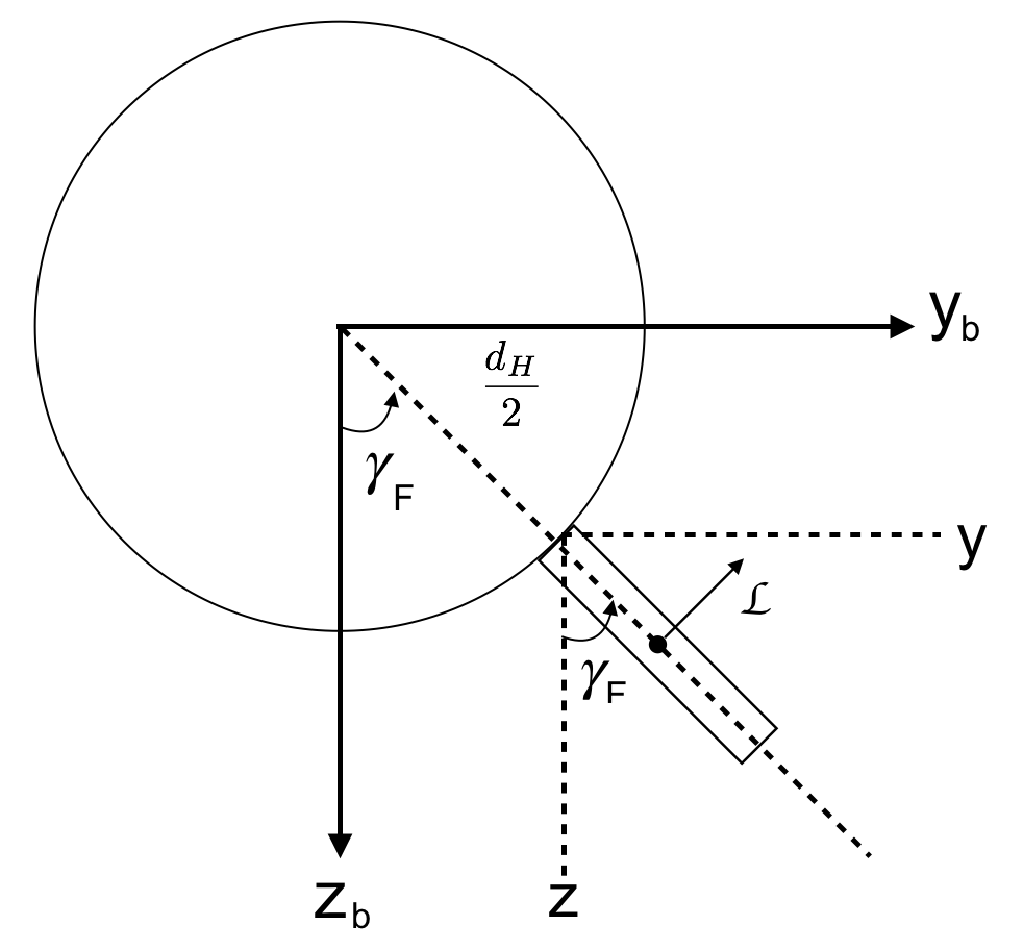
\includegraphics[width=0.4\textwidth]{FinLocation2.eps}
\caption{Definition of fin geometric parameters}	
\label{FIG:FinLocation}
\end{figure}
%\begin{figure}
%\centering
%\begin{tikzpicture}[x=1.5cm,y=1.5cm,>=latex']
%	\coordinate (O) at (-1,-1);
%	\draw[black,fill=black] (-1,-1) circle (.5ex) 
%	\coordinate (OD) at(0,-1);
%	% plot the x-axis
%	\draw [dashed] (O) -- (-1,1.5);
%	\draw [->] (O) -- (-1,1.5);
%	\draw [->] (O) -- (2,-1) node[pos=0.1] {\small ${CO}$};;
%	\draw [dashed] (O) -- (-1,-3);
%	\draw [dashed] (O) -- (-2,-1);
%	\draw (-2,1)--(0,1);
%	\draw (-2,-3)--(0,-3);
%	\draw (-2,1)--(-2,-3);
%	\draw (0,1)--(0,-3);
%	\end{tikzpicture}
%\caption{Modeling of hull as hollow cylinder} \label{fig:HullModeling}
%\end{figure}
Fins are modeled as rectangle with length $a_{F}$ and width $b_{F}$. Assume the side edge $b_{F}$ is directly attached on the hull surface. Then we represent the position and the orientation of the fins in the hull cylindrical coordinate system. As illustrated in Figure \ref{FIG:FinLocation}, $x_{F}$ is defined as the x-coordinate of fin geometric center in body frame $\lbrace b \rbrace$. We rotate the $xz$-plane of the robot body frame in the counterclockwise direction by angle $\gamma_{F}$ until the fin geometric center located in this plane. Consequently, the i-th fin geometric center vector $\vec{r}_{F,i}$ can be written as
\begin{align}
\vec{r}_{F,i}=
\begin{pmatrix}
x_{F,i} \\
0.5(d_{H}+a_{F,i})\sin(\gamma_{F,i}) \\
0.5(d_{H}+a_{F,i})\cos(\gamma_{F,i})
\end{pmatrix}
\end{align}
in body frame $\lbrace b \rbrace$.
Then we can calculate the center cross product vector as 
\begin{align}
 \vec{r}_{F,i}\times&=
 \begin{pmatrix}
   0&-\dfrac{1}{2}(d_{H}+a_{F,i})\cos(\gamma_{F,i})&\dfrac{1}{2}(d_{H}+a_{F,i})\sin(\gamma_{F,i})\\
   \dfrac{1}{2}(d_{H}+a_{F,i})\cos(\gamma_{F,i})&0&-x_{F,i}\\
   -\dfrac{1}{2}(d_{H}+a_{F,i})\sin(\gamma_{F,i})&x_{F,i}&0
 \end{pmatrix}.
\end{align}
In the following, we use $\vec{e}_{1}=[0\quad 0 \quad 1]^{T}$, $\vec{e}_{2}=[0 \quad 1\quad 0]^{T}$ and $\vec{e}_{3}=[1\quad 0 \quad 0]^{T}$ to represent unit vectors in the body frame $\lbrace b \rbrace$ and $n_{f}$ to denote the number of control fins. 
For each fin, the lift $L$ and drag $D$ of fins can be calculated as
\begin{align}
\vec{L}_{ i }(\alpha _{ i }):=a_{F,i}b_{F,i}{ C }_{ L }(\alpha _{ i })Q(U_{fin})\begin{pmatrix} 0 \\ cos({ \gamma  }_{ F,i }) \\ -sin({ \gamma  }_{ F,i }) \end{pmatrix}
\end{align}
\begin{align}
\vec{D}_{ i }(\alpha _{ i })=S{ C }_{ D }(\alpha _{ i })Q(U_{fin})\vec{e}_{1},
\end{align}
where $a_{F,i}$ and $b_{F,i}$ are the length and width of the i-th fin, respectively. $C_{L}$ is the lift coefficient of fin and $C_{D}$ is the drag coefficient. 
$Q(U_{fin})=0.5\rho U_{fin}^{2}$ is a short notation for simplicity.  $U_{fin}$ is the magnitude of fin middle point velocity vector relative to the surrounding fluid in the body frame $\lbrace b \rbrace$ and $U_{fin}=\sqrt{u_{fin}^{2}+v_{fin}^{2}+w_{fin}^{2}}$.

If the surge velocity is dominant, that is, $u$ is much bigger than $v$ and $w$, the previous formulas for calculating the lift and drag can be rewritten as
\begin{align}
\vec{L}_{ i }(\alpha _{ i }):=a_{F,i}b_{F,i}{ C }_{ L }(\alpha _{ i })Q(u_{fin})\begin{pmatrix} 0 \\ cos({ \gamma}_{ F,i}) \\ -sin({ \gamma  }_{ F,i }) \end{pmatrix}
\end{align}
\begin{align}
\vec{D}_{ i }(\alpha _{ i })=S{ C }_{ D }(\alpha _{ i })Q(u_{fin})\vec{e}_{1}.
\end{align}

It turns out the resultant force vector produced by $n_{f}$ fins can be calculated as follows: 
\begin{align}
\vec{f}_{F}(\alpha_{i} )=\begin{pmatrix} \sum _{ i=1 }^{ n_{f} }{ \vec{L}_{ i }(\alpha _{ i })^{ T }\vec{e}_{ 1 }+ } \sum _{ i=1 }^{ n_{f} }{ \vec{D}_{ i }(\alpha _{ i })^{ T }\vec{e}_{ 1 } }  \\ \sum _{ i=1 }^{ n_{f} }{\vec{L}_{ i }(\alpha _{ i })^{ T }\vec{e}_{ 2 }+ } \sum _{ i=1 }^{ n_{f} }{ \vec{D}_{ i }(\alpha _{ i })^{ T }\vec{e}_{ 2 } }  \\ \sum _{ i=1 }^{ n_{f} }{ \vec{L}_{ i }(\alpha _{ i })^{ T }\vec{e}_{ 3 }+ } \sum _{ i=1 }^{n_{f} }{ \vec{D}_{ i }(\alpha _{ i })^{ T }\vec{e}_{ 3 } }  \end{pmatrix}.
\end{align}
The resultant torque vector is calculated as:
\begin{align}
\vec{\tau} _{F}(\alpha_{i} )=\sum _{ i=1 }^{n_{f}}{ \vec{r}_{F,i} \times \vec{L}_{i}(\alpha_{i}) } +\sum _{ i=1 }^{n_{f}}{ \vec{r}_{F,i} \times \vec{D}_{i}(\alpha_{i})}.
\end{align}  
\begin{figure}
\includegraphics[width=0.8\textwidth]{SmallAOA.eps}
\caption{Small angle of attack assumption~\cite{FinModeling}}	
\label{FIG:smallAOA}
\end{figure}
For small angle of attack $\alpha$, as depicted in Figure \ref{FIG:smallAOA}, it is reasonable to approximate the lift and drag coefficients as
\begin{align}
C_{L}(\alpha_{i})=c_{L}\alpha_{i},
\end{align}    
\begin{align}
C_{D}(\alpha_{i})=c_{D}\alpha_{i}^{2},
\end{align}
where $c_{L}$, $c_{D}$ are fin-specific parameters estimated from experiments. For the following calculations, we adopt this assumption.
The drag moment of the $i$-th fin is calculated as
\begin{align}
&\vec{r}_{F,i}\times \emph{\textbf{D}}_{i}(\alpha_{i})= \nonumber \\
&\begin{pmatrix}
   0&-\dfrac{1}{2}(d_{H}+a_{F,i})\cos(\gamma_{F,i})&\dfrac{1}{2}(d_{H}+a_{F,i})\sin(\gamma_{F,i})\\
   \dfrac{1}{2}(d_{H}+a_{F,i})\cos(\gamma_{F,i})&0&-x_{F,i}\\
   -\dfrac{1}{2}(d_{H}+a_{F,i})\sin(\gamma_{F,i})&x_{F,i}&0
 \end{pmatrix} 
 \begin{pmatrix}
 c_{D}a_{F,i}b_{F,i}Q(u_{fin})\alpha_{i}^{2} \\0\\0
 \end{pmatrix} \nonumber \\
&=\begin{pmatrix}
0 \\
\dfrac{1}{2}(d_{H}+a_{F,i})\cos(\gamma_{F,i})c_{D}a_{F,i}b_{F,i}Q(u_{fin}) \\
-\dfrac{1}{2}(d_{H}+a_{F,i})\sin(\gamma_{F,i})c_{D}a_{F,i}b_{F,i}Q(u_{fin})
\end{pmatrix}
\alpha_{i}^{2}.
\end{align}
The lift moment is given by
\begin{align}
&\vec{m}_{F,i}=\vec{r}_{F,i}\times \emph{\textbf{L}}_{i}(\alpha_{i})= \nonumber \\
&\begin{pmatrix}
   0&-\dfrac{1}{2}(d_{H}+a_{F,i})\cos(\gamma_{F,i})&\dfrac{1}{2}(d_{H}+a_{F,i})\sin(\gamma_{F,i})\\
   \dfrac{1}{2}(d_{H}+a_{F,i})\cos(\gamma_{F,i})&0&-x_{F,i}\\
   -\dfrac{1}{2}(d_{H}+a_{F,i})\sin(\gamma_{F,i})&x_{F,i}&0
 \end{pmatrix} 
 \begin{pmatrix}
 0\\c_{L}a_{F,i}b_{F,i}Q(u_{fin})\cos(\gamma_{F,i})\alpha_{i}\\
c_{L}a_{F,i}b_{F,i}Q(u_{fin})\sin(\gamma_{F,i})\alpha_{i}
 \end{pmatrix} \nonumber \\
&=\begin{pmatrix}
-c_{L}a_{F}b_{F}Q(u_{fin})\dfrac{1}{2}(d_{H}+a_{F})\\
c_{L}a_{F}b_{F}Q(u_{fin})x_{F}\sin(\gamma_{F})\\
c_{L}a_{F}b_{F}Q(u_{fin})x_{F}\cos(\gamma_{F})
\end{pmatrix}
\alpha_{i}.
\end{align}
Note that the moment of fins should be calculated according the center of mass $CG$ of the whole robot, that is, $ \vec{r}_{F,i} $ here should be the vector connecting the center of fins and the center of mass $CG$. However, we assume that, for calculating the fin moments, the center of mass of the robot is the origin $CO$ of the body frame $\lbrace b \rbrace$. It means that the vector $\vec{r}_{F,i}$ denotes the position of fin geometric center in the robot body frame.

We use the lift force generated by fins as the control input and treat the drag as disturbance.

Similar to the defined mapping vector of thrusters, we also define the mapping vector for fins as follows:
\begin{align}
\emph{\textbf{B}}_{F}=
\begin{pmatrix}
0\\c_{L}a_{F}b_{F}Q(u_{fin})\cos(\gamma_{F})\\
c_{L}a_{F}b_{F}Q(u_{fin})\sin(\gamma_{F})\\
-c_{L}a_{F}b_{F}Q(u_{fin})\dfrac{1}{2}(d_{H}+a_{F})\\
c_{L}a_{F}b_{F}Q(u_{fin})x_{F}\sin(\gamma_{F})\\
c_{L}a_{F}b_{F}Q(u_{fin})x_{F}\cos(\gamma_{F})
\end{pmatrix}\in \mathbb{R}^{6}.\label{EQ:FinMappingVector}
\end{align}
The fin mapping matrix is not only geometry-dependent but also state dependent, since it contains the surge velocity term $Q(u_{fin})$. For small drift angle, the angle of attack $\alpha$ of the hydrofoils can be approximated by the mechanic
al angle of rotation of the hydrofoils~\cite{Fossen2008}. For our case, it means $\alpha=\delta_{F}$, where $\delta_{F}$ is the deflection angle of fins. Then the generalized force generated by fins can be written in the following form:
\begin{align}
\vec{\tau}_{F}=
\begin{pmatrix}
\vec{f}_{F}\\ \vec{m}_{F}
\end{pmatrix}=
\emph{\textbf{B}}_{F}\delta_{F}.
\end{align}

\section{Dynamics Construction}
The moments of inertia for each individual modules making up the robot is calculated with respect to the module's own frame, where the hull frame is usually chosen as the robot body frame $\lbrace b \rbrace$. It means, the elemental moments of inertia should be transformed to the body frame $\lbrace b \rbrace$. For each submodule whose center of gravity $ CG_{s} $ is $(x_{s}, y_{s}, z_{s})^{T}$ in body frame $\lbrace b \rbrace$, we can compute their moments of inertia in $\lbrace b \rbrace$ as follows: 
\begin{align}
I_{xx,s}^{b}=I_{xx,s}+m_{s}(y_{s}^{2}+z_{s}^{2}),\label{EQ:MomentTransfer1}
\end{align}
\begin{align}
I_{yy,s}^{b}=I_{yy,s}+m_{s}(z_{s}^{2}+x_{s}^{2}),\label{EQ:MomentTransfer2}
\end{align}
\begin{align}
I_{zz,s}^{b}=I_{zz,s}+m_{s}(x_{s}^{2}+y_{s}^{2}).\label{EQ:MomentTransfer3}
\end{align}
where $I_{xx,s}^{b}, I_{yy,s}^{b} and I_{zz,s}^{b}$ are moments of inertia with respect to the body axes $\lbrace b \rbrace$ of the component $s$. In this work, we only consider the moment of inertia of batteries, hull enclosure and the constant moment of inertia of all devices within the hull, the moments of inertia of fins, thrusters and other components are neglected.

Suppose we have totally $N$ components, then the resultant center of mass $ \vec{r}_{G} $ for the whole robot is 
\begin{align}
\vec{r}_{G}=\dfrac{\sum_{s=1}^{N}m_{s}\vec{r}_{G,s}}{\sum_{s=1}^{N}m_{s}},\label{EQ:CGAll}
\end{align} 
where $m_{s}$ is the mass of the component $s$, and $\vec{r}_{G,s}$ is the position vector of the component $s$ in the body frame $\lbrace b \rbrace$.

\section{Estimation of the Hydrodynamic Effects}
Hydrodynamic effects are the distinct feature for underwater robots. Strictly speaking, each component (hull, thrusters and fins) contributes to the hydrodynamic forces and moments. However, hydrodynamic effects depend not only on the geometric structure but also on the working condition (e.g. the inflow fluid velocity). Normally, the underwater robot dynamics is built in body frame (usually the geometric center of the hull). However, the hydrodynamic effect of each module is calculated with respect to its own geometric center. It means they should be transformed into body frame according to their positions. This transformation will make the nonlinear and strongly coupled hydrodynamic effects more complicated. Thus, the basic assumption for the estimation is that only hull contributes significantly to the hydrodynamic coefficients, while other contributions are negligible. Because we set the hull frame as the robot body frame, no transformation is needed. The hydrodynamic effects include mainly two parts: the added mass and the hydrodynamic damping. 

\subsection{Estimating the Added Mass Coefficients}
For estimating the added mass, we assume that the added mass of thrusters and fins are negligible and only the added mass of the cylindrical hull is taken into consideration. For a symmetrical cylindrical rigid body of mass $m_{H}$ with circular section of radius $r_{H}$ and length $l_{H}$, the added mass coefficients (definitions in Section~\ref{addedmassdefi}) can be derived theoretically by applying the strip theory as follows:
\begin{align}
X_{\dot{u}}=-0.1m_{H},
\end{align}
\begin{align}
Y_{\dot{v}}=-\pi\rho r_{H}^{2}l_{H},
\end{align}
\begin{align}
Z_{\dot{w}}=-\pi\rho r_{H}^{2}l_{H},
\end{align}
\begin{align}
K_{\dot{p}}=0,
\end{align}
\begin{align}
M_{\dot{q}}=-\dfrac{1}{12}\pi\rho r_{H}^{2}l_{H}^{3},
\end{align}
\begin{align}
N_{\dot{r}}=-\dfrac{1}{12}\pi\rho r_{H}^{2}l_{H}^{3}.
\end{align}
The cylindrical hull has three planes of symmetry. When the robot is completely submerged in the fluid, the added mass matrix $\emph{\textbf{M}}_{A}$ and the Coriolis matrix $\emph{\textbf{C}}_{A}$ can be calculated as follows:
\begin{align}
\emph{\textbf{M}}_{A}=diag([-X_{\dot{u}} -Y_{\dot{v}} -Z_{\dot{w}}
-K_{\dot{p}} -M_{\dot{q}} -N_{\dot{r}}]) \label{EQ:AddedMassMatrix}
\end{align}
\begin{align}
\emph{\textbf{C}}_{A}=
\begin{pmatrix}
0&0&0&0&-Z_{\dot{w}}w&Y_{\dot{v}}v\\
0&0&0&Z_{\dot{w}}w&0&-X_{\dot{u}}u\\
0&0&0&-Y_{\dot{v}}v&X_{\dot{u}}u&0\\
0&-Z_{\dot{w}}w&Y_{\dot{v}}v&0&-N_{\dot{r}}\dot{r}&M_{\dot{q}}q\\
Z_{\dot{w}}w&0&-X_{\dot{u}}u&N_{\dot{r}}r&0&-K_{\dot{p}}p\\
-Y_{\dot{v}}v&X_{\dot{u}}u&0&-M_{\dot{q}}q&K_{\dot{p}}p&0
\end{pmatrix}. \label{EQ:CoriolisMatrix}
\end{align}
\nm{$\emph{\textbf{C}}_{A}$}{Added Coriolis Matrix}

The total mass matrix is
\begin{align}
\emph{\textbf{M}}=\emph{\textbf{M}}_{RB}+\emph{\textbf{M}}_{A}.
\end{align}
Since $\emph{\textbf{M}}_{RB}\succ 0$ and $\emph{\textbf{M}}_{A}\succeq 0$, the complete robot inertia matrix is positive definite, i.e., $\emph{\textbf{M}}\succ 0$, thus $\emph{\textbf{M}}$ is invertible.  


%The vehicle is approximated as an ellipsoid characterized by the parametric representation:
% \begin{align}
% \dfrac{x^{2}}{a^{2}}+\dfrac{y^{2}}{b^{2}}+\dfrac{z^{2}}{c^{2}}=1
% \end{align} 
% where $b=c$ and $a>c$, and the eccentricity $e_{c}=1-(b/a)^{2}$. Then % the ellipsoid can be rewritten as
% \begin{align}
% \dfrac{x^{2}}{a^{2}}+\dfrac{y^{2}+z^{2}}{b^{2}}=1
% \end{align}





% Being $b=c$ and $a>c$, it can be noticed that a prolate spheroid  
% The rigid body matrix
% \begin{align}
% \emph{\textbf{M}}^{CO}_{RB} &=
% \begin{pmatrix}
% m\emph{\textbf{I}}_{3\times 3}&-m\emph{\textbf{S}}(\vec{r}_{g}^{b}) \\
% m\emph{\textbf{S}}(\vec{r}_{g}^{b})&
% \emph{\textbf{I}}_{g}-m\emph{\textbf{S}}^{2}(\vec{r}^{b}_{g})
% \end{pmatrix}
% \end{align}
% The eccentricity is defined as 
% \begin{align}
% e_{c}=1-(b/a)^{2}
% \end{align} 
% \begin{align}
% \alpha_{0}=\dfrac{2(1-e_{c}^{2})(\dfrac{1}{2}\log\left(\dfrac{1+e_{c}}{1-e_{c}}\right)-e_{c})}{e_{c}^{3}}
% \end{align}
% \begin{align}
% \beta_{0}=\dfrac{1}{e_{c}^{2}}-\dfrac{(1-e_{c}^{2})\log\left(\dfrac{1+e_{c}}{1-e_{c}}\right)}{2e_{c}^{3}}
% \end{align}
% Based on these two parameters 
% \begin{align}
% X_{\dot{u}}=-m\dfrac{\alpha_{0}}{2-\alpha_{0}}
% \end{align}
% \begin{align}
% Y_{\dot{v}}=-m\dfrac{\beta_{0}}{2-\beta_{0}}
% \end{align}
% \begin{align}
% Z_{\dot{w}}=Y_{\dot{v}}
% \end{align}
% \begin{align}
% M_{\dot{q}}=-\dfrac{m}{5}\dfrac{(b^{2}-a^{2})^{2}(\alpha_{0}-\beta_{0})}{2(b^{2}-a^{2})-(b^{2}+a^{2})(\alpha_{0}-\beta_{0})}
% \end{align}
% \begin{align}
% N_{\dot{r}}=M_{\dot{q}}
% \end{align}

\subsection{Estimating the Damping Coefficients}
The hydrodynamic damping can be modeled as:
\begin{align}
F_{H}=-\dfrac{1}{2}\rho C_{D}A_{r}|\nu|\nu, 
\end{align}
where $\rho$ is the fluid density, $C_{D}$ is the drag coefficient, $A_{r}$ the reference area, and $\nu$ is an arbitrary linear or angular velocity.
% The drag coefficient is a function of the Reynolds number $Re$, which is % defined as
% \begin{align}
% Re=\dfrac{vl}{\nu}.
% \end{align}
% where $v$ is the velocity of the fluid (SI units: $m/s$), $l$ is the % characteristic linear dimension ($m$) and $\nu$ is the kinematic viscosity of %the fluid ($m^{2}/s$). 
To estimate the drag coefficient of the robot hull, we make the following the assumptions:
\begin{enumerate}
\item The drag coefficient $C_{D}$ is dependent on the Reynolds number $Re$, the Mach number $Ma$ and the direction of the flow. Low Mach number is assumed, in this case the drag coefficient is independent of it. We also assume high speed manoeuvring where the incoming flow direction is more-or-less the same and the drag coefficient $C_{D}$ can be treated as a constant~\cite{wikiDragCoefficient}.
\item The skin friction is neglected.
\item The underwater robot is performing a non-coupled motion.
\item The quadratic damping terms are dominant.
\item The lift force of the hull is not considered.
\end{enumerate}
The damping matrix is defined as
\begin{align}
\emph{\textbf{D}}=
diag([-X_{u|u|}|u|,-Y_{v|v|}|v|,-Z_{w|w|}|w|,-K_{p|p|}|p|,-M_{q|q|}|q|,-N_{r|r|}|r|]).
\end{align}
The damping coefficient in the x-direction due to the viscous force acting on the frontal area is given as 
\begin{align}
X_{|u|u}=-\dfrac{1}{2}\rho C_{D}A_{frontal}=-\dfrac{1}{2}\rho\pi C_{D}r_{H}^{2},
\end{align}
The damping coefficients in the y and z axes due to viscous effects on the side projected areas of the hull is given as
\begin{align}
Y_{|v|v}=-\dfrac{1}{2}\rho C_{D}2r_{H}l_{H}
\end{align}
and 
\begin{align}
Z_{w|w|}=-\dfrac{1}{2}\rho C_{D}2r_{H}l_{H}
\end{align}
respectively.

%The rotation drag is neglected since for stable underwater robot motion, %angular velocities are very small. 

% The drag coefficient $ X_{u|u|}=-0.5\rho \pi a^{2}C_{d}$ and $Y_{v|v|}=Z_{w|% w|}=X_{u|u|}\dfrac{a}{b}$.

%The rigid body Coriolis Matrix can be written componentwise as follows:
%\begin{align}
%\begin{pmatrix}
%0&0&0&-m(y_{g}q+z_{g}r)
%\end{pmatrix}
%\end{align} 
%\begin{gather}\label{EQ:RigidCoriolis}
%\emph{\textbf{C}}_{RB}(\vec{\upsilon})=
%\left(
%\begin{matrix} 
%0&0&0 \\
%0&0&0 \\
%0&0&0 \\
%-m(y_{g}+z_{g}r)&m(y_{g}p+w)&m(z_{g}p-v)\\
%m(x_{g}q-w)&-m(z_{g}r+x_{g}p)&m(z_{g}q+u)\\
%m(x_{g}r+v)&m(y_{g}r-u)&-m(x_{g}p+y_{g}q)
%\end{matrix}
%\right.
% \nonumber\\
%\qquad \qquad\left. 
%\begin{matrix} {m(y_{g}q+z_{g}r)} & {-m(x_{g}q-w)} & {-m(x_{g}r+v)} \\
%-m(y_{g}p+w) & m(z_{g}r+x_{g}p) & -m(y_{g}r-u) \\
%-m(z_{g}p-v) & -m(z_{g}q+u) & m(x_{g}p+y_{g}q) \\
%0 & -I_{yz}q-I_{xz}p+I_{z}r & I_{yz}r+I_{xy}p-I_{y}q \\
%I_{yz}q+I_{xz}p-I_{z}r &0& -I_{xz}r-I_{xy}q+I_{x}p \\
%-I_{yz}r-I_{xy}p+I_{y}q&I_{xz}r+I_{xy}q-I_{x}p &0 
%\end{matrix}
%\right)
%\end{gather}
The hull has no contribution to the roll moment, hence 
\begin{align}
K_{p|p|}=0.
\end{align}
   
The drag force due to pitch motion is given as
\begin{align}
M_{q|q|}q|q|=-\dfrac{1}{2}\rho w|w| \int^{l_{H}/2}_{-l_{H}/2}C_{D}~2r~dx~x
\end{align}
For small angular motions, $w\approx q x$. Thus, the pitch damping coefficient is given by
\begin{align}
M_{q|q|}=-\dfrac{1}{12}\rho C_{D} r_{H}l_{H}^{4}
\end{align}
Similarly, the horizontal drag forces contribute the yaw drag, whose coefficient is same as the pitch drag:
\begin{align}
N_{r|r|}=-\dfrac{1}{12}\rho C_{D} r_{H}l_{H}^{4}
\end{align}
The details for derivation of these parameters can be found in~\cite{Sia1999}, it also includes the drag caused by thrusters and struct linking hull and thruster which could be for future work. With help of two geometric parameters $l_{H}$ and $r_{H}$, the hydrodynamic terms in the robot dynamic equation including $\emph{\textbf{M}}_{A}$, $\emph{\textbf{C}}_{A}$ and $\emph{\textbf{D}}$ can be computed.

To sum up, in this chapter we model the robot hull, batteries, fins as simple geometric shapes determined by several geometric parameters. In addition, for thrusters we only pay attention on their positions, motor orientations and spin directions regardless of their shapes. By means of this modeling method, we are able to construct a customizable robot dynamics parametrized with these geometric parameters. They will be chosen as decision variables for the robot geometry optimization so that the current dynamics can be computed at each optimization iteration. 
%____________________________________________________
\chapter{Path Planning for Underwater Robots}
%For path planning with trim trajectory and Frenet-Serret frame, the sway- and heave velocities are always equal to zero. The roll-, pitch and yaw velocities are relatively small with respect to the surge velocity. Thus, we can approximate the velocity of fin relative to the fluid $U_{fin}$ as the surge velocity $u_{fin}$ of the robot. 
% Given the nonlinear system $\dot{\vec{x}}=\vec{f}(\vec{x},\vec{u})$ and a desired trajectory $(\vec{x}_{d},\vec{u}_{d})$. We want to design a controller in the form $\vec{u}=\alpha(\vec{x},\vec{x}_{d},\vec{u}_{d})$ such that $\lim_{t \to \infty}x-x_{d}=0$. Since underwater robots are affine in commanded inputs, the dynamics can be simplified as $\vec{f}(\vec{x},\vec{u})=\vec{f}(\vec{x})+\vec{g}(\vec{x})\vec{u}$. Let us define new error state $\vec{x}-\vec{x}_{d}$ and $\vec{v}=\vec{u}-\vec{u}_{d}$ and we can calculate the error dynamics:
% \begin{align}
% \dot{\vec{e}}=\dot{\vec{x}}-\dot{\vec{x}}_{d}=\vec{f}(\vec{x})+\vec{g}(\vec{x})\vec{u}-\vec{f}(\vec{x}_{d})-\vec{g}(\vec{x}_{d})\vec{u}_{d}
% \\
% =\vec{f}(\vec{e}+\vec{x}_{d})-\vec{f}(\vec{x}_{d})+\vec{g}(\vec{e}+\vec{x}_{d})(\vec{v}+\vec{u}_{d})-\vec{g}(\vec{x}_{d})\vec{u}_{d} 
% \\
% =\vec{F}(\vec{e}+\vec{v},\vec{x}_{d}(t),\vec{u}_{d}(t))
% \end{align}
% For tracking the desired trajectory, we can assume the error $\vec{e}$ is very small if our controller works very well so that we can linearize around $\vec{e}=\vec{0}$: 
% \begin{align}
% \dot{\vec{e}}=\emph{\textbf{A}}(t)\vec{e}+\emph{\textbf{B}}(t)\vec{v}
% \end{align}
%where $ \emph{\textbf{A}}(t)=\dfrac{\partial \vec{F}}{\partial \vec{e}}\Bigr|_{\vec{x}_{d}(t),\vec{u}_{d}(t)} $ and $ \emph{\textbf{B}}(t)=\dfrac{\partial \vec{F}}{\partial \vec{v}}\Bigr|_{\vec{x}_{d}(t),\vec{u}_{d}(t)} $. It is often the case that $\emph{\textbf{A}}$ depend on $ \vec{x}_{d} $. Hence, we can rewrite $ \emph{\textbf{A}}(t)=\emph{\textbf{A}}(\vec{x}_{d})$ and $ \emph{\textbf{B}}(t)=\emph{\textbf{B}}(\vec{x}_{d})$. We can design  a state feedback controller $ \emph{\textbf{K}}(\vec{x}_{d}) $ for each $\vec{x}_{d}$. Then we can stabilize the system using the feedback 
% \begin{align}
% \vec{v}=\emph{\textbf{K}}(\vec{x}_{d})\vec{e}
% \end{align}
% Substituting back, the controller can be written as
% \begin{align}
% \vec{u}=\emph{\textbf{K}}(\vec{x}_{d})(\vec{x}-\vec{x}_{d})+\vec{u}_{d}
% \end{align}

% Given the desired trajectory $\vec{\eta}_{1,d}(t)=[x_{d}(t),y_{d}(t),z_{d}(t)]^{T}$. We can calculate the desired orientation $\vec{\eta}_{2,d}(t)=[\phi_{d}(t),\theta_{d}(t),\psi_{d}(t)]^{T}$  
% \begin{align}
% \vec{\eta}_{1,d}^{i}(t) \rightarrow \vec{\eta}_{2,d}^{i}(t) \rightarrow \vec{\upsilon}_{d}^{b}(t) \rightarrow \vec{\upsilon}_{d}^{b}(t) \rightarrow \vec{\upsilon}_{fin,d}^{b}(t) \rightarrow \vec{\upsilon}_{fin,d}^{f}(t)
% \end{align}

% \begin{align}
% \alpha_{d}(t)=atan2(\vec{\upsilon}_{fin,d}^{f}(t)(3),\vec{\upsilon}_{fin,d}^{f}(t)(1)) \rightarrow C_{L}(\alpha_{d}(t)), C_{D}(\alpha_{d}(t))
% \end{align}
%The flow frame depends on the attack angle and is therefore a function of velocity $\vec{\upsilon}_{d}^{b}(t)$ and  can be represented as $\emph{\textbf{R}}^{flow}_{f}(\vec{\upsilon}_{d}^{b}(t))$
%The configuration can be determined by three parameters: body-fixed tilt angle $\theta_{tilt}$ and the unitary vector $\vec{\lambda}_{F}$ which determine the rotation matrix from body frame to fin frame  and force exerting point on fins $CF$
%\begin{align}
%\emph{\textbf{R}}^{f}_{b}=
%\cos(\theta_{tilt})\emph{\textbf{I}}
%+(1-\cos(\theta_{tilt}))\vec{\lambda}\vec{\lambda}^{T}
%-\sin(\theta_{tilt})\emph{\textbf{S}}(\vec{\lambda})
%\end{align}

%Thus, lift and drag of fins are dependent explicitly on the desired velocity trajectory $\vec{\upsilon}_{d}^{b}$ and implicitly on time $t$.
Underwater robots are used in practice to perform rescue tasks, to monitor the environment or to explore mysterious deep sea world. The success of these jobs requires an efficient trajectory planning. One important novelty of this work is that we propose kinematic and dynamic specifications from the trajectories. Due to the convenience for analysis and control design, trim trajectories will be chosen for our problem.     
 

\section{Trim Trajectory}
The trim trajectory comes originally from path planning for aircraft. It facilitates the planning and control problem since it corresponds to a stable states. The vehicle motion is uniform in the body frame under trim condition, i.e., the surge, sway, heave, roll, pitch and yaw velocities stay constant within one trim segment. For our case, the linearized error dynamics between the desired trim trajectory segment and the real one is unique after a specific nonlinear transformation (discussed in Chapter 4) so that we are able to use the analysis and design methods for LTI system to design the optimization algorithm. This will be discussed in the next chapter.

\begin{figure}
\includegraphics[width=0.8\textwidth]{TrimTrajectory.eps}
\caption{Trim trajectory}	
\label{FIG:TrimTrajectory}
\end{figure}
  
A trim trajectory can be parameterized by three parameters, which can be denoted as
\begin{align}
\vec{\eta}_{\mathcal{T}}:\left(||\vec{v}_{\mathcal{T}}||,\dot{\psi}_{\mathcal{T}},\gamma_{\mathcal{T}}\right)^{T}
\end{align}
where $\vec{v}_{\mathcal{T}}$ is the trim speed. For Frenet-Serret frames $\lbrace FS \rbrace$, the trim speed is equal to the surge velocity $u$. The angle $\gamma_{\mathcal{T}}$ is the motion path angle, for aircraft it is the so-called flight path angle. The trim yaw angle is given by $ \psi_{\mathcal{T}}(t)=\dot{\psi}_{\mathcal{T}}t+\psi_{0} $ where $ \dot{\psi}_{\mathcal{T}}\in \mathbb{R} $ is the constant yaw rate and $\psi_{0}\in \left[0,2\pi\right)$ is the initial yaw angle. Along the trim trajectory, the roll angle and pitch angle remain unchanged, i.e., $\dot{\phi}_{\mathcal{T}}=0$ and $\dot{\theta}_{\mathcal{T}}=0$. 
\begin{align}
\dot{\vec{\eta}}_{\mathcal{T}}=||\vec{v}_{\mathcal{T}}||
\begin{pmatrix}
\cos(\gamma)_{\mathcal{T}}\cos(\psi_{\mathcal{T}}(t)-\psi_{v}) \\
\sin(\gamma)_{\mathcal{T}}\cos(\psi_{\mathcal{T}}(t)-\psi_{v}) \\
-\sin(\gamma_{\mathcal{T}})
\end{pmatrix}.
\end{align}
$\psi_{v}$ is the angle between the robot's heading and the velocity vector. Because we use Frenet-Serret frame discussed in the next section, the vehicle's heading is coincided with the velocity vector, the angle $\psi_{v}$ should be equal to zero.
Integrating the above equation shows that a trim trajectory segment corresponds to a helix with radius $||\vec{v}_{\mathcal{T}}||\dot{\psi}_{\mathcal{T}}^{-1}\cos(\gamma_{\mathcal{T}})$ parameterized by
\begin{align}
\vec{\eta}_{\mathcal{T}}(t)=||\vec{v}_{\mathcal{T}}||\dot{\psi}_{\mathcal{T}}^{-1}\cos(\gamma)
\begin{pmatrix}
\sin(\psi_{\mathcal{T}}(t)-\psi_{v})-\sin(\psi_{0}-\psi_{v}) \\
\cos(\psi_{\mathcal{T}}(t)-\psi_{v})+\cos(\psi_{0}-\psi_{v}) \\
-\dot{\psi}_{\mathcal{T}}\tan(\gamma_{\mathcal{T}})t
\end{pmatrix}+
\vec{\eta}_{0}
\end{align}
where $\vec{\eta}_{0}=[x_{0},y_{0},z_{0}]^{T} \in \mathbb{R}^{3}$ is the initial trim trajectory position. 
As illustrated in figure~\ref{FIG:PathAngle}, the motion path angle $\gamma_{\mathcal{T}}$ is equal to the sum of the angle of attack $\alpha$ and the trim pitch angle $\theta_{\mathcal{T}}$, i.e., $\gamma_{\mathcal{T}}=\alpha+\theta_{\mathcal{T}}$. After implementing the Frenet-Serret frame for the trajectory frame, the robot velocity vector should be coincided with the x-axis of the robot body frame $\lbrace b \rbrace$, meaning that the angle of attack $\alpha$ is equal to zero, and $\gamma_{\mathcal{T}}=\theta_{\mathcal{T}}$.
\begin{figure}
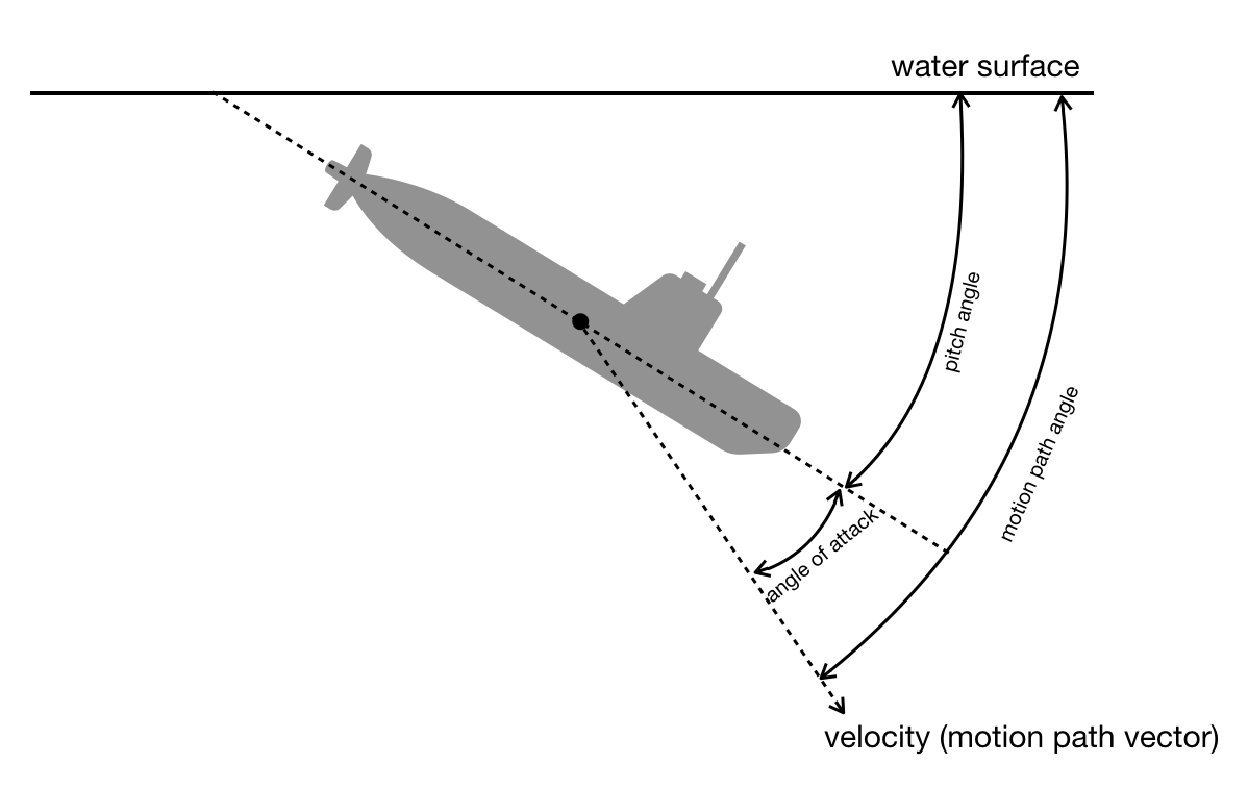
\includegraphics[width=0.85\textwidth]{PathAngle.eps}
\caption{Trajectory angles}	
\label{FIG:PathAngle}
\end{figure}
\section{Frenet-Serret Frame}
The underwater robots have six dynamic variables (3 linear velocities and 3 angular velocities) and six kinematic variables (positions and Euler angles in inertial frame $\lbrace i \rbrace$), all of which fully describes the robot's behaviour together. The trim trajectory merely offer us the information about the desired kinematic position, we still lack the data about the desired orientation (Euler angles) and the desired velocities along these trim trajectories. The Frenet-Serret model has the advantage of being a well-established means of modeling continuous spatial curves. The definition of the Frenet-Serret frame is elaborated in follows: 

When a particle moves along a continuous, differentiable curve in three-dimensional Euclidean space $\mathbb{R}^{3}$, its motion can be characterized by three unit vectors: $\vec{T}^{i}(t)$, $\vec{N}^{i}(t)$ and $\vec{B}^{i}(t)$. $\vec{T}^{i}(t)$ is a unit vector tangent to the curve, denoting the motion direction. 
\begin{align}
\vec{T}^{i}(t)=\dfrac{\vec{\eta}_{\mathcal{T}}^{'}(t)}{||\vec{\eta}_{\mathcal{T}}^{'}(t)||}.
\end{align}    
The normal vector $\vec{N}^{i}(t)$ is equal to the derivative with respect to the arclength parameter of the curve divided by its length which can be calculated as follows:
\begin{align}
\vec{N}^{i}(t)=\dfrac{\vec{T}^{'}(t)}{||\vec{T}^{'}(t)||}=
\dfrac{\vec{\eta}_{\mathcal{T}}^{'}(t)\times (\vec{\eta}_{\mathcal{T}}^{''}(t)\times \vec{\eta}_{\mathcal{T}}^{'}(t))}{||\vec{\eta}_{\mathcal{T}}^{'}(t)||\cdot||\vec{\eta}_{\mathcal{T}}^{''}(t)\times \vec{\eta}_{\mathcal{T}}^{'}(t))||}.
\end{align}
The binomal vector $\vec{B}^{i}(t)$ is the cross product of the normal vector $\vec{N}^{i}(t)$ and the tangent vector $\vec{T}^{i}(t)$ and is calculated as 
\begin{align}
\vec{B}^{i}(t)=\vec{T}^{i}(t) \times \vec{N}^{i}(t)=
\dfrac{\vec{\eta}_{\mathcal{T}}^{''}(t)\times \vec{\eta}_{\mathcal{T}}^{'}(t)}{||\vec{\eta}_{\mathcal{T}}^{''}(t)\times \vec{\eta}_{\mathcal{T}}^{'}(t))||}.
\end{align}
These three vectors are expressed in inertial world frame $\left\lbrace i \right\rbrace$ because they describe the kinematic property of the robot. $\vec{T}^{i}(t)$, $\vec{N}^{i}(t)$ and $\vec{B}^{i}(t)$ constitute an orthonormal basis spanning in $\mathbb{R}^{3}$ and we use $\left\lbrace FS\right\rbrace$ to denote the Frenet-Serret frame.

The transformation matrix from the Frenet-Serret frame to the inertial world frame $\lbrace i \rbrace$ is defined as
\begin{align}
 \emph{\textbf{R}}_{FS}^{i} &=
 (\vec{T}^{i}(t) \quad \vec{N}^{i}(t) \quad \vec{B}^{i}(t)) \nonumber \\
 &=
 \begin{pmatrix}
c\psi_{\mathcal{T}} c\theta_{\mathcal{T}}&-s\psi_{\mathcal{T}} c\phi_{d}+c\psi_{\mathcal{T}} s\theta_{\mathcal{T}} s\phi_{\mathcal{T}}&s\psi_{\mathcal{T}} s\phi_{\mathcal{T}}+c\psi_{\mathcal{T}} c\phi_{\mathcal{T}} s\theta_{\mathcal{T}} \\
s\psi_{\mathcal{T}} c\theta_{\mathcal{T}}&c\psi_{\mathcal{T}} c\phi_{\mathcal{T}}+s\phi_{\mathcal{T}} s\theta_{\mathcal{T}} s\psi_{\mathcal{T}}&-c\psi_{\mathcal{T}} c\phi_{\mathcal{T}}+s\theta_{\mathcal{T}} s\psi_{\mathcal{T}} c\phi_{\mathcal{T}}\\
-s\theta_{\mathcal{T}}&c \theta_{\mathcal{T}} s \phi_{\mathcal{T}}&c \theta_{\mathcal{T}} c\phi_{\mathcal{T}}
\end{pmatrix}
\end{align}
Thus, we can calculate the desired orientation (Euler angles) $\vec{\lambda}_{\mathcal{T}}=(\phi_{\mathcal{T}},~\theta_{\mathcal{T}},
~\psi_{\mathcal{T}})^{T}$ along the trim trajectory as follows:
\begin{align}
\theta_{\mathcal{T}}=-\sin^{-1}(\vec{T}^{i}(t)),
\end{align}
\begin{align}
\phi_{\mathcal{T}}=-\sin^{-1}(\sec(\theta_{\mathcal{T}})\cdot \vec{N}^{i}(t))
\end{align}
The desired yaw angle comes from the definition of the trim trajectory:
\begin{align}
\psi_{\mathcal{T}}=\dot{\psi}_{\mathcal{T}}t+\psi_{0}.
\end{align}
In the previous discussions, we have derived the complete desired kinematic states $\vec{\eta}_{\mathcal{T}}=(\vec{p}_{\mathcal{T}},~\vec{\lambda}_{\mathcal{T}})^{T}$ for underwater robots for the trim trajectory. The desired dynamic states can be determined 
from the kinematics with help of the rotation  matrix $ \emph{\textbf{R}}_{FS}^{i}$.

For a given trim trajectory, we can calculate the desired velocities as follows:
\begin{align}
\vec{\upsilon}_{\mathcal{T}}=
\begin{pmatrix}
\vec{v}_{\mathcal{T}} \\
\vec{\omega}_{\mathcal{T}}
\end{pmatrix}=
(\emph{\textbf{R}}_{FS}^{i})^{-1}.
\end{align}

In conclusion, the 12 state variables $\vec{x}_{\mathcal{T}}=(\vec{\eta}_{\mathcal{T}}$,~$\vec{\upsilon}_{\mathcal{T}})^{T}$ fully specify the kinematics and dynamics the robot should perform along the trim trajectory. We will use the desired states to derive the error dynamics in the next chapter.



\chapter{Trajectory Tracking Error Dynamics}

The underwater robot system is a strongly coupled nonlinear system. Traditionally, the underwater robot dynamics is lineazied about constant states with specific values. For instance, in~\cite{F2011} (pp.174), low-speed application is assumed for neutrally buoyant submersible. Thus, the nonlinear Coriolis, centripetal, damping, restoring and buoyancy forces and moments can be linearized about $\vec{\upsilon}=\vec{0}$ and $\phi=\theta=0$. The linearized manoeuvring model (\cite{F2011}, pp.131)  for marine craft is based on the assumption of constant cruise speed $U$. Also, the nonlinear damping is approximated by a linear damping matrix. 

In this  work, we present a path-based linearization method for the error dynamics between robot's real states and the path-determined states. Our method is in essence also linearization about constant states. Nevertheless, our linearization is based on all dynamic (velocities) and kinematic (position and Euler angles) states except for the yaw angle $\psi$ instead several of them. Therefore, we bring nearly the full information of the trajectory into the linearized model. Furthermore, we do not require explicit values for these states. In other words, our linearized model is a function of the states. For a specific trim trajectory, we evaluate the function with explicit values from the trajectory specifications. The state variables of underwater robots can be divided into two groups, i.e., kinematic states and dynamic states. Dynamic states include three linear and three angular velocities represented in the robot frame $\lbrace b \rbrace$:
\begin{align}
\vec{x}_{dyn}=\vec{\upsilon}=
\begin{pmatrix}
\vec{v}\\ \vec{\omega}
\end{pmatrix}=
\begin{pmatrix}
u\\v\\w\\p\\q\\r
\end{pmatrix}
\in 
\mathbb{R}^{6}.
\end{align}
Kinematic states consist of the position and orientation of the underwater robot in the inertial world frame $\lbrace i \rbrace$:
\begin{align}
\vec{x}_{kin}=\vec{\eta}=
\begin{pmatrix}
\vec{p} \\ \vec{\lambda}
\end{pmatrix}=
\begin{pmatrix}
x \\ y \\ z \\ \phi \\ \theta\\ \psi
\end{pmatrix}
\in 
\mathbb{R}^{6}.
\end{align}
The whole states are defined as:
\begin{align}
\vec{x}=
\begin{pmatrix}
\vec{x}_{dyn}\\ \vec{x}_{kin}
\end{pmatrix}
\in 
\mathbb{R}^{12}.
\end{align}
The state space representation $\mathcal{P}$ of nonlinear underwater robot system can be written in the following form:
\begin{align}
\mathcal{P}
\coloneqq
\dfrac{d}{dt}
\begin{pmatrix}
\vec{x}_{dyn} \\
\vec{x}_{kin}
\end{pmatrix}=
\begin{pmatrix}
\mathfrak{F}_{dyn}(\vec{x}_{dyn},\vec{x}_{kin})\\
\mathfrak{F}_{kin}(\vec{x}_{dyn},\vec{x}_{kin})
\end{pmatrix}+
\begin{pmatrix}
\mathfrak{B}(\vec{x}_{dyn})\mathfrak{H}(\vec{x}_{dyn},\vec{u})\\0
\end{pmatrix}
\end{align}
Now, we want to reformulate the standard underwater robot equations of motion
\begin{align}
\emph{\textbf{M}}\dot{\vec{\upsilon}}+\emph{\textbf{C}}(\vec{\upsilon})\vec{\upsilon}+\emph{\textbf{D}}(\vec{\upsilon})\vec{\upsilon}+\vec{g}(\vec{\eta})=\vec{\tau}
\label{EQ:Dy}
\end{align}
into the aforementioned form.


More precisely, we want to identify all the terms in the following equations from the robot dynamics and kinematics. 
\begin{empheq}[left=\mathcal{P}:\empheqlbrace]{align}
& \dfrac{d}{dt}\vec{v}=\mathfrak{F}_{\vec{v}}(\vec{v},\vec{\omega})+\mathfrak{F}_{\vec{v}}^{\lambda}(\Pi_{i}\vec{\lambda})+\mathfrak{B}_{\vec{v}}(\vec{v},\vec{\omega})\mathfrak{H}(\vec{v},\vec{u}) \label{EQ:P1}\\
&\dfrac{d}{dt}\vec{\omega}=\mathfrak{F}_{\vec{\omega}}(\vec{v},\vec{\omega})+\mathfrak{F}_{\omega}^{\lambda}(\Pi_{i}\vec{\lambda})+\mathfrak{B}_{\omega}(\vec{v},\vec{\omega})\mathfrak{H}(\vec{v},\vec{u}) \label{EQ:P2} \\
& \dfrac{d}{dt}\vec{p}=\emph{\textbf{R}}(\lambda)\vec{v} \label{EQ:P3} \\
&\dfrac{d}{dt}\vec{\lambda}=\emph{\textbf{Q}}(\Pi_{i}\vec{\lambda})\vec{\omega}\label{EQ:P4}.
\end{empheq}
where $\vec{\lambda}$ represents the Euler angles ($\phi$, $\theta$, $\psi$) and $\Pi_{i}\vec{\lambda}=(\phi, \theta)^{T}$ denotes the two kinematic states appearing in the underwater robot dynamics since the restoring term $\vec{g}(\eta)$ includes the two angles. $\emph{\textbf{R}}(\lambda)$ is the linear velocity transformation matrix and $\emph{\textbf{Q}}(\Pi_{i}\vec{\lambda})$ is the angular velocity transformation matrix. 
The dynamic equation \ref{EQ:Dy} can be rewritten as 
\begin{align}
\dot{\vec{\upsilon}}=-\emph{\textbf{M}}^{-1}\emph{\textbf{C}}(\vec{\upsilon})\vec{\upsilon}-\emph{\textbf{M}}^{-1}\emph{\textbf{D}}(\vec{\upsilon})\vec{\upsilon}-\emph{\textbf{M}}^{-1}\emph{\textbf{g}}(\vec{\eta})+\emph{\textbf{M}}^{-1}\tau.
\end{align}
Note that the inertia matrix $\emph{\textbf{M}}$ is the sum of the rigid body inertia matrix $\emph{\textbf{M}}_{RB}$ and the added mass inertia matrix $\emph{\textbf{M}}_{A}$, the Coriolis matrix $\emph{\textbf{C}}(\vec{\upsilon})$ includes the rigid body Coriolis matrix $\emph{\textbf{C}}_{RB}(\vec{\upsilon})$ and the added mass Coriolis matrix $\emph{\textbf{C}}_{A}$. 
We assign the first three rows of the rigid body added mass $\emph{\textbf{C}}_{RB}(\vec{v},\vec{\omega})$ matrix into sub-matrices $\emph{\textbf{C}}_{RB,\vec{v}}(\vec{v},\vec{\omega})$ and the last three rows into sub-matrices $\emph{\textbf{C}}_{RB,\vec{\omega}}(\vec{v},\vec{\omega})$:
\begin{align}
\emph{\textbf{C}}_{RB,\vec{v}}(\vec{v},\vec{\omega})=
\begin{pmatrix}
0&0&0&m(y_{g}q+z_{g}r)&-m(x_{g}q-w)&-m(x_{g}r+v)\\
0&0&0&-m(y_{g}p+w)&m(z_{g}r+x_{g}p)&-m(y_{g}r-u)\\
0&0&0&-m(z_{g}p-v)&-m(z_{g}q+u)&m(x_{g}p+y_{g}q)\\
\end{pmatrix} \label{EQ:CoriolisRigidBodyV}
\end{align}
and
\begin{gather}\label{EQ:CoriolisRigidBodyW}
\emph{\textbf{C}}_{RB,\vec{\omega}}(\vec{v},\vec{\omega})=
\left(
\begin{matrix} -m(y_{g}+z_{g}r)&m(y_{g}p+w)&m(z_{g}p-v)\\
m(x_{g}q-w)&-m(z_{g}r+x_{g}p)&m(z_{g}q+u)\\
m(x_{g}r+v)&m(y_{g}r-u)&-m(x_{g}p+y_{g}q)
\end{matrix}
\right.
 \nonumber\\
\qquad \qquad\left. \begin{matrix} 
0 & -I_{yz}q-I_{xz}p+I_{z}r & I_{yz}r+I_{xy}p-I_{y}q \\
I_{yz}q+I_{xz}p-I_{z}r &0& -I_{xz}r-I_{xy}q+I_{x}p \\
-I_{yz}r-I_{xy}p+I_{y}q&I_{xz}r+I_{xy}q-I_{x}p &0  \end{matrix}
\right).
%\end{equation}
\end{gather}
Similarly, the added mass Coriolis matrix can be also divided into two parts $\emph{\textbf{C}}_{A,\vec{v}}(\vec{v},\vec{\omega})$ and $\emph{\textbf{C}}_{A,\vec{\omega}}(\vec{v},\vec{\omega})$, where
\begin{align}
\emph{\textbf{C}}_{A,\vec{v}}(\vec{v},\vec{\omega})=
\begin{pmatrix}
0&0&0&0&-Z_{\dot{w}}w&Y_{\dot{v}}v\\
0&0&0&Z_{\dot{w}}w&0&-X_{\dot{u}}u\\
0&0&0&-Y_{\dot{v}}v&X_{\dot{u}}u&0
\end{pmatrix}
\end{align} 
and
\begin{align}
\emph{\textbf{C}}_{A,\vec{\omega}}(\vec{v},\vec{\omega})=
\begin{pmatrix}
0&-Z_{\dot{w}}w&Y_{\dot{v}}v&0&-N_{\dot{r}}\dot{r}&M_{\dot{q}}q\\
Z_{\dot{w}}w&0&-X_{\dot{u}}u&N_{\dot{r}}r&0&-K_{\dot{p}}p\\
-Y_{\dot{v}}v&X_{\dot{u}}u&0&-M_{\dot{q}}q&K_{\dot{p}}p&0
\end{pmatrix}.
\end{align}
For the drag matrix, we perform the same separation:
\begin{align}
\emph{\textbf{D}}_{\vec{v}}=
\begin{pmatrix}
-X_{u|u|}|u|&0&0&0&0&0\\
0&-Y_{v|v|}|v|&0&0&0&0\\
0&0&-Z_{w|w|}|w|&0&0&0\\
\end{pmatrix}
\end{align}
\begin{align}
\emph{\textbf{D}}_{\vec{\omega}}=
\begin{pmatrix}
0&0&0&-K_{p|p|}|p|\\
0&0&0&0&-M_{q|q|}|q|\\
0&0&0&0&0&-N_{r|r|}|r|\\
\end{pmatrix}.
\end{align}
The restoring term 
\begin{align}
\vec{g}(\vec{\eta})=
\begin{pmatrix}
(W-B)\sin(\theta)\\
-(W-B)\cos(\theta)\sin(\phi)\\
-(W-B)\cos(\theta)\cos(\phi)\\
-(y_{g}W-y_{b}B)\cos(\theta)\cos(\phi)+(z_{g}W-z_{b}B)\cos(\theta)\sin(\phi)\\
(z_{g}W-z_{b}B)\sin(\theta)+(x_{g}W-x_{b}B)\cos(\theta)\cos(\phi)\\
-(x_{g}W-x_{b}B)\sin(\theta)\cos(\phi)-(y_{g}W-y_{b}B)\sin(\theta)
\end{pmatrix} \label{EQ:Restoring}
\end{align}
can also be separated into the following two terms
\begin{align}
\vec{g}_{\vec{v}}(\vec{\eta})=
\begin{pmatrix}
(W-B)\sin(\theta)\\
-(W-B)\cos(\theta)\sin(\phi)\\
-(W-B)\cos(\theta)\cos(\phi)
\end{pmatrix} \label{EQ:RestoringV}
\end{align}
\begin{align}
\vec{g}_{\vec{\omega}}(\vec{\eta})=
\begin{pmatrix}
-(y_{g}W-y_{b}B)\cos(\theta)\cos(\phi)+(z_{g}W-z_{b}B)\cos(\theta)\sin(\phi)\\
(z_{g}W-z_{b}B)\sin(\theta)+(x_{g}W-x_{b}B)\cos(\theta)\cos(\phi)\\
-(x_{g}W-x_{b}B)\sin(\theta)\cos(\phi)-(y_{g}W-y_{b}B)\sin(\theta)
\end{pmatrix},\label{EQ:RestoringW}
\end{align}
where $W$ is the total weight of the robot, and $B$ denotes the total buoyancy. $\vec{r}_{g}=(x_{g}, y_{g}, z_{g})^{T}$ is the center of gravity vector and $\vec{r}_{b}=(x_{b}, y_{b}, z_{b})^{T}$ is the center of buoyancy vector.
After reordering the Coriolis matrix, the damping matrix and the restoring matrix and comparing them with~\ref{EQ:P1} and~\ref{EQ:P2}, we can obtain the following equations:
\begin{align}
\mathfrak{F}_{\vec{v}}(\vec{v},\vec{\omega})=
-\emph{\textbf{M}}^{-1}(\emph{\textbf{C}}_{RB,\vec{v}}+\emph{\textbf{C}}_{A,\vec{v}}+\emph{\textbf{D}}_{\vec{v}})
\end{align}
\begin{align}
\mathfrak{F}_{\vec{\omega}}(\vec{v},\vec{\omega})=
-\emph{\textbf{M}}^{-1}(\emph{\textbf{C}}_{RB,\vec{\omega}}+\emph{\textbf{C}}_{A,\vec{\omega}}+\emph{\textbf{D}}_{\vec{\omega}})
\end{align}
\begin{align}
\mathfrak{F}_{\vec{\omega}}^{\vec{\lambda}}(\Pi_{i}\vec{\lambda})=
-\emph{\textbf{M}}^{-1}\vec{g}_{\vec{\omega}}(\vec{\eta})
\end{align}
\begin{align}
\mathfrak{F}_{\vec{v}}^{\vec{\lambda}}(\Pi_{i}\vec{\lambda})=
-\emph{\textbf{M}}^{-1}\vec{g}_{\vec{v}}(\vec{\eta}).
\end{align}
Now, let us come to the input part, $\vec{u}$ is the control input generated by fins and thrusters. Suppose we have $n_{t}$ thrusters and $n_{f}$ fins, then it can be written as 
\begin{align}
\vec{u}=(u_{T,1}\cdots u_{T,n_{t}}~ \delta_{F,1} \cdots \delta_{F,n_{f}})^{T}\in \mathbb{R}^{(n_{t}+n_{f})\times 1}. 
\end{align}
For each actuator there is a corresponding input mapping vector and we can formulate the input matrix as $\emph{\textbf{B}}_{a}=(\emph{\textbf{B}}_{T,1} \cdots \emph{\textbf{B}}_{T,n_{t}}~\emph{\textbf{B}}_{F,1} \cdots \emph{\textbf{B}}_{F,n_{f}})\in \mathbb{R}^{6\times(n_{t}+n_{f})}$.
The first three rows of the matrix $\emph{\textbf{B}}_{a}$ are denoted by $\emph{\textbf{B}}_{a,f}\in \mathbb{R}^{3\times(n_{t}+n_{f})}$ and the last three rows of the matrix are represented by $\emph{\textbf{B}}_{a,m}\in \mathbb{R}^{3\times(n_{t}+n_{f})}$. The generalized force generated by the actuators can be represented as $\vec{\tau}=\emph{\textbf{B}}_{a}\vec{u}$. Separately written, $\vec{f}=\emph{\textbf{B}}_{a,f}\vec{u}$ and $\vec{m}=\emph{\textbf{B}}_{a,m}\vec{u}$, where $\vec{f}$ is the force vector along x-, y- and z- axes and $\vec{m}$ is the moment vector about x-, y- and z-axes of the body frame $\lbrace b \rbrace$.

Hence, for our modeling methods, 
\begin{align}
\mathfrak{B}_{\vec{v}}(\vec{v},\vec{\omega})\mathfrak{H}(\vec{v},\vec{u})=
\emph{\textbf{M}}^{-1}\emph{\textbf{B}}_{a,f}\vec{u},
\end{align}
\begin{align}
\mathfrak{B}_{\vec{\omega}}(\vec{v},\vec{\omega})\mathfrak{H}(\vec{v},\vec{u})=
\emph{\textbf{M}}^{-1}\emph{\textbf{B}}_{a,m}\vec{u}.
\end{align}

This finishes the transformation of the robot dynamics into standard state space form.
\section{Nonlinear Transformation and Error Dynamics}
Figure~\ref{FIG:FrameRelationship} shows the relationship between different frames, the $\lbrace i \rbrace$ denotes the inertial world frame, and $\emph{\textbf{R}}$ represents the coordinate transformation from $\lbrace i \rbrace$ to the real robot frame $\lbrace b \rbrace$. $\lbrace \mathcal{T} \rbrace$ denotes the Frenet-Serret frame along the trim trajectory, ideally the robot body frame $\lbrace b \rbrace$ should coincide with the the frame $\lbrace \mathcal{T} \rbrace$ for a perfect tracking, but it is not necessarily the case in reality. Thus, we use $\emph{\textbf{R}}_{E}$ to denote the transformation matrix from the body frame $\lbrace b \rbrace$ to the trim frame $\lbrace \mathcal{T} \rbrace$ and $\emph{\textbf{R}}_{\mathcal{T}}$ to denote the transformation matrix from the trim frame $\lbrace \mathcal{T} \rbrace$ to the inertial world frame $\lbrace i \rbrace$. Based on these definitions, we have the following relationship:
\begin{align}
\emph{\textbf{R}}_{E}=\emph{\textbf{R}}^{-1}_{\mathcal{T}}\emph{\textbf{R}}.
\end{align}     
\begin{figure}
\center
\begin{tikzpicture}
\node (A) at (0,0){$\lbrace i \rbrace$};
\node (B) at (3,3){$\lbrace b \rbrace$};
\node (C) at (6,0){$\lbrace \mathcal{T} \rbrace$};
\draw[->, very thick] (B) to
node[above] {$\emph{\textbf{R}}$} (A);
\draw[->, very thick] (C) to
node[above] {$\emph{\textbf{R}}_{\mathcal{T}}$} (A);
\draw[->, very thick] (B) to
node[above] {$\emph{\textbf{R}}_{E}$} (C);
\end{tikzpicture}
\caption{Frame relationship}	
\label{FIG:FrameRelationship}
\end{figure}
The desired states can be calculated from the predefined reference trim trajectories. Now we want to formulate the error dynamics. The velocities errors are defined intuitively as the difference between the desired velocity and the real velocity:
\begin{align}
\vec{v}_{E}=\vec{v}-\vec{v}_{\mathcal{T}}, \label{EQ:NLT1}
\end{align}
\begin{align}
\vec{\omega}_{E}=\vec{\omega}-\vec{\omega}_{\mathcal{T}}. \label{EQ:NLT2}
\end{align}
The position and orientation are defined in the inertial world frame $\lbrace i \rbrace$. We want to observe all the errors in the body frame $\lbrace b \rbrace$
\begin{align}
\vec{p}_{E}=\emph{\textbf{R}}^{-1}(\vec{p}-\vec{p}_{\mathcal{T}}) \label{EQ:NLT3}
\end{align}
\begin{align}
\vec{\lambda}_{E}=\emph{\textbf{Q}}^{-1}(\vec{\lambda}-\vec{\lambda}_{\mathcal{T}}) \label{EQ:NLT4}
\end{align}
Since the desired velocities $\vec{\upsilon}_{\mathcal{T}}$ and $\vec{\omega}_{\mathcal{T}}$ are constant along the trim trajectory, then we can obtain the following relationships for the derivative of velocity errors:
\begin{align}
\dfrac{d}{dt}\vec{v}_{E}=\dfrac{d}{dt}\vec{v}-\dfrac{d}{dt}\vec{v}_{\mathcal{T}}=\dfrac{d}{dt}\vec{v}
\end{align}
\begin{align}
\dfrac{d}{dt}\vec{\omega}_{E}=\dfrac{d}{dt}\vec{\omega}-\dfrac{d}{dt}\vec{\omega}_{\mathcal{T}}=\dfrac{d}{dt}\vec{\omega}.
\end{align}
In the following, we study the error kinematics.
We start from the nonlinear position transformation equation. 
\begin{align}
\vec{p}_{E}&=\emph{\textbf{R}}^{-1}(\vec{p}-\vec{p}_{\mathcal{T}}) \Rightarrow\nonumber \\
\vec{p}_{\mathcal{T}}&=\vec{p}-\emph{\textbf{R}}\vec{p}_{E}.
\end{align}
Taking derivative of both sides, we obtain 
\begin{align}
\dfrac{d}{dt}\vec{p}_{\mathcal{T}}=\dfrac{d}{dt}\vec{p}-(\dfrac{d}{dt}\emph{\textbf{R}})\vec{p}_{E}-\emph{\textbf{R}}(\dfrac{d}{dt}\vec{p}_{E}).
\end{align}
Since $\dfrac{d}{dt}\emph{\textbf{R}}(\vec{\lambda})=\emph{\textbf{R}}(\vec{\lambda})\emph{\textbf{S}}(\vec{\omega})$, we have the following equation:
\begin{align}
\dfrac{d}{dt}\vec{p}_{\mathcal{T}}=\dfrac{d}{dt}\vec{p}-\emph{\textbf{R}}\emph{\textbf{S}}(\vec{\omega})\vec{p}_{E}-\emph{\textbf{R}}(\dfrac{d}{dt}\vec{p}_{E}).
\end{align}
Reforming it, we get
\begin{align}
\emph{\textbf{R}}_{\mathcal{T}}\vec{v}_{\mathcal{T}}=\emph{\textbf{R}}\vec{v}-\emph{\textbf{R}}
\emph{\textbf{S}}(\vec{\omega})\vec{p}_{E}-\emph{\textbf{R}}\dfrac{d}{dt}\vec{p}_{E}.
\end{align}
Premultiplying both sides by $\emph{\textbf{R}}^{-1}$ and using $ \emph{\textbf{R}}_{E}^{-1}=\emph{\textbf{R}}^{-1}\emph{\textbf{R}}_{\mathcal{T}}$
\begin{align}
\dfrac{d}{dt}\vec{p}_{E}=\vec{v}-\emph{\textbf{R}}_{E}^{-1}\vec{v}_{\mathcal{T}}
-\emph{\textbf{S}}(\vec{\omega})\vec{p}_{E}
\end{align}
For the orientation error, we take the first derivative of the orientation transformation equation
\begin{align}
\vec{\lambda}_{E}&=\emph{\textbf{Q}}^{-1}(\vec{\lambda}-\vec{\lambda}_{\mathcal{T}}) \nonumber \\ \Rightarrow
\dfrac{d}{dt}\vec{\lambda}_{E}&=\emph{\textbf{Q}}^{-1}(\dfrac{d}{dt}\vec{\lambda}-\dfrac{d}{dt}\vec{\lambda}_{\mathcal{T}})+(\dfrac{d}{dt}\emph{\textbf{Q}}^{-1})(\vec{\lambda}-\vec{\lambda}_{\mathcal{T}}).
\end{align}
Since 
\begin{align}
\dfrac{d}{dt}\vec{\lambda}=\emph{\textbf{Q}}\vec{\omega}
\end{align}
and 
\begin{align}
\dfrac{d}{dt}\vec{\lambda}_{\mathcal{T}}=\emph{\textbf{Q}}_{\mathcal{T}}
\vec{\omega}_{\mathcal{T}},
\end{align}
we obtain 
\begin{align}
\dfrac{d}{dt}\vec{\lambda}_{E}=\emph{\textbf{Q}}^{-1}\emph{\textbf{Q}}\vec{\omega}
-\emph{\textbf{Q}}^{-1}\emph{\textbf{Q}}_{\mathcal{T}}
\vec{\omega}_{\mathcal{T}}
+(\dfrac{d}{dt}\emph{\textbf{Q}}^{-1})(\vec{\lambda}-\vec{\lambda}_{\mathcal{T}})\Rightarrow \nonumber \\
\dfrac{d}{dt}\vec{\lambda}_{E}=\vec{\omega}
-\emph{\textbf{Q}}^{-1}\emph{\textbf{Q}}_{\mathcal{T}}
\vec{\omega}_{\mathcal{T}}
+(\dfrac{d}{dt}\emph{\textbf{Q}}^{-1})\emph{\textbf{Q}}\vec{\lambda}_{E}
\end{align}

To sum up, the nonlinear error dynamic model $ \mathcal{P}_{E} $ for a given trim trajectory set is formulated as follows:
\begin{empheq}[left=\mathcal{P}_{E}:\empheqlbrace]{align}
&\dfrac{d}{dt}\vec{v}_{E}=\mathfrak{F}_{\vec{v}}(\vec{v},\vec{\omega})+\mathfrak{F}_{\vec{v}}^{\vec{\lambda}}(\Pi_{i}\vec{\lambda})+\mathfrak{B}_{\vec{v}}(\vec{v},\vec{\omega})\mathfrak{H}(\vec{v},\vec{u}) \\
&\dfrac{d}{dt}\vec{\omega}_{E}=\mathfrak{F}_{\vec{\omega}}(\vec{v},\vec{\omega})+\mathfrak{F}_{\vec{\omega}}^{\vec{\lambda}}(\Pi_{i}\vec{\lambda})+\mathfrak{B}_{\vec{\omega}}(\vec{v},\vec{\omega})\mathfrak{H}(\vec{v},\vec{u})\\
&\dfrac{d}{dt}\vec{p}_{E}=\vec{v}-\emph{\textbf{R}}_{E}^{-1}\vec{v}_{\mathcal{T}}
-\emph{\textbf{S}}(\vec{\omega}_{\mathcal{T}})\vec{p}_{E}\\
&\dfrac{d}{dt}\vec{\lambda}_{E}=\vec{\omega}
-\emph{\textbf{Q}}^{-1}\emph{\textbf{Q}}_{\mathcal{T}}
\vec{\omega}_{\mathcal{T}}
+(\dfrac{d}{dt}\emph{\textbf{Q}}^{-1})\emph{\textbf{Q}}\vec{\lambda}_{E}.
\end{empheq}
We define the the error dynamics input as
\begin{align}
\vec{u}_{E}=\vec{u}-\vec{u}_{\mathcal{T}},
\end{align} 
where the $\vec{u}$ is the control input for the nonlinear robot dynamics, and $\vec{u}_{\mathcal{T}}$ is the desired trim input. Since for the trim trajectory, the desired trim velocities, the desired trim roll angle and the desired trim pitch angle are constant meaning that $\dot{\vec{\upsilon}}_{\mathcal{T}}=0$ and the restoring term $\vec{g}(\vec{ \eta})$ depends only on $\Pi_{i}\vec{\lambda}$, we obtain
\begin{align}
\vec{\tau}_{\mathcal{T}}=
\emph{\textbf{M}}\dot{\vec{\upsilon}}_{\mathcal{T}}+\emph{\textbf{C}}(\vec{\upsilon}_{\mathcal{T}})\vec{\upsilon}_{\mathcal{T}}+\emph{\textbf{D}}(\vec{\upsilon}_{\mathcal{T}})\vec{\upsilon}_{\mathcal{T}}+\vec{g}(\vec{\eta}_{\mathcal{T}}) \nonumber \\
=\emph{\textbf{C}}(\vec{\upsilon}_{\mathcal{T}})\vec{\upsilon}_{\mathcal{T}}+\emph{\textbf{D}}(\vec{\upsilon}_{\mathcal{T}})\vec{\upsilon}_{\mathcal{T}}+\vec{g}(\Pi_{i}\vec{\lambda}_{\mathcal{T}}), \label{EQ:desiredtau}
\end{align}
and 
\begin{align}
\vec{u}_{\mathcal{T}}=\emph{\textbf{B}}_{a}^{-1}\vec{\tau}_{\mathcal{T}}\label{EQ:desiredu}
\end{align}
The nonlinear transformation procedure is depicted in Figure~\ref{FIG:NonlinearTransform}.  

\begin{figure}
\includegraphics[width=0.9\textwidth]{NonlinearPlant.eps}
\caption{Nonliear transformation and error dynamics formulation}	
\label{FIG:NonlinearTransform}
\end{figure}
\section{Linearization of Error Dynamics}
\label{LinearizationMethods}
In the previous section, we have derived the error dynamic model for a given trim trajectory segment. In this section, we want to prove that the linearization for a specific trim trajectory segment $\vec{\eta}_{\mathcal{T}}$ is unique.

Firstly, we linearize the velocities error and get the following
equations:
\begin{empheq}[left=\empheqlbrace]{align}
&\dfrac{d}{dt}\delta\vec{v}_{E}=\emph{\textbf{A}}_{\vec{v}}^{\vec{v}}
\delta\vec{v}_{E}+\emph{\textbf{A}}_{\vec{v}}^{\vec{\omega}}
\delta\vec{\omega}_{E}+\emph{\textbf{A}}_{\vec{v}}^{\vec{\lambda}}
\delta\vec{\lambda}_{E}+\emph{\textbf{B}}_{\vec{v}}\delta\vec{u} \\
&\dfrac{d}{dt}\delta\vec{\omega}_{E}=\emph{\textbf{A}}_{\vec{\omega}}^{\vec{v}}
\delta\vec{v}_{E}+\emph{\textbf{A}}_{\vec{\omega}}^{\vec{\omega}}
\delta\vec{\omega}_{E}+\emph{\textbf{A}}_{\vec{\omega}}^{\vec{\lambda}}
\delta\vec{\lambda}_{E}+\emph{\textbf{B}}_{\vec{\omega}}\delta\vec{u} 
\end{empheq} 
where
\begin{empheq}[left=\empheqlbrace]{align}
&\emph{\textbf{A}}_{\vec{v}}^{\vec{v}}=\dfrac{\partial}{\partial \vec{v}}[\mathfrak{F}_{\vec{v}}(\vec{v},\vec{\omega})+\mathfrak{B}_{\vec{v}}(\vec{v},\vec{\omega})\mathfrak{H}(\vec{v},\vec{u})]
 \\
&\emph{\textbf{A}}_{\vec{v}}^{\vec{\omega}}=\dfrac{\partial}{\partial \vec{\omega}}[\mathfrak{F}_{v}(\vec{v},\vec{\omega})+\mathfrak{B}_{\vec{v}}(\vec{v},\vec{\omega})\mathfrak{H}(\vec{v},\vec{u})]
\\
&\emph{\textbf{A}}_{\vec{v}}^{\vec{\lambda}}=\dfrac{\partial}{\partial \vec{\lambda}}\mathfrak{F}_{\vec{v}}^{\vec{\lambda}}(\Pi_{i}\vec{\lambda})\\
&\emph{\textbf{B}}_{\vec{\upsilon}}=\dfrac{\partial}{\partial \vec{u}}
\mathfrak{B}_{\vec{v}}(\vec{v},\vec{\omega})\mathfrak{H}(\vec{v},\vec{u})
\end{empheq} 
and
\begin{empheq}[left=\empheqlbrace]{align}
&\emph{\textbf{A}}_{\vec{\omega}}^{\vec{v}}=\dfrac{\partial}{\partial \vec{v}}[\mathfrak{F}_{\omega}(\vec{v},\vec{\omega})+\mathfrak{B}_{\vec{\omega}}(\vec{v},\vec{\omega})\mathfrak{H}(\vec{v},\vec{u})]
 \\
&\emph{\textbf{A}}_{\vec{\omega}}^{\vec{\omega}}=\dfrac{\partial}{\partial \vec{\omega}}[\mathfrak{F}_{\omega}(\vec{v},\vec{\omega})+\mathfrak{B}_{\vec{\omega}}(\vec{v},\vec{\omega})\mathfrak{H}(\vec{v},\vec{u})]
\\
&\emph{\textbf{A}}_{\vec{\omega}}^{\vec{\lambda}}=\dfrac{\partial}{\partial \vec{\lambda}}\mathfrak{F}_{\vec{\omega}}^{\vec{\lambda}}(\Pi_{i}\vec{\lambda})\\
&\emph{\textbf{B}}_{\vec{\omega}}=\dfrac{\partial}{\partial \vec{u}}
\mathfrak{B}_{\vec{\omega}}(\vec{v},\vec{\omega})\mathfrak{H}(\vec{v},\vec{u}).
\end{empheq} 
Next, we want to show that the linearization of the position error $\vec{p}_{E}$ is time-invariant.
We define 
\begin{align}
\vec{f}_{\vec{p}_{E}}=\vec{v}
-\emph{\textbf{R}}_{E}^{-1}\vec{v}_{\mathcal{T}}
-\emph{\textbf{S}}(\vec{\omega}_{\mathcal{T}})\vec{p}_{E}
\end{align}
\begin{align}
\dfrac{d}{dt}\delta\vec{p}_{E}=
\underbrace{\dfrac{\partial \vec{f}_{\vec{p}_{E}}}{\partial \vec{v}_{E}}}_{(1)}\cdot\delta \vec{v}_{E}+
\underbrace{\dfrac{\partial \vec{f}_{\vec{p}_{E}}}{\partial \vec{\omega}_{E}}}_{(2)}\cdot\delta \vec{\omega}_{E}+
\underbrace{\dfrac{\partial \vec{f}_{\vec{p}_{E}}}{\partial \vec{p}_{E}}}_{(3)}\cdot\delta \vec{p}_{E}+
\underbrace{\dfrac{\partial \vec{f}_{\vec{p}_{E}}}{\partial \vec{\lambda}_{E}}}_{(4)}\cdot\delta \vec{\lambda}_{E}\label{EQ:PE1}
\end{align}
We calculate these four terms separately. 
Since $\vec{v}_{E}=\vec{v}-\vec{v}_{\mathcal{T}}$ and $\vec{v}_{\mathcal{T}}$ is a constant, we have
\begin{align}
(1):\dfrac{\partial \vec{f}_{\vec{p}_{E}}}{\partial \vec{v}_{E}}=\emph{\textbf{I}}_{3 \times 1}.\label{EQ:PE2}
\end{align}
\begin{align}
(2):\dfrac{\partial \vec{f}_{\vec{p}_{E}}}{\partial \vec{\omega}_{E}}=\emph{\textbf{0}}_{3 \times 1}.\label{EQ:PE3}
\end{align}
\begin{align}
(3):\dfrac{\partial \vec{f}_{\vec{p}_{E}}}{\partial \vec{p}_{E}}=
-\dfrac{\partial}{\partial \vec{p}_{E}}(\emph{\textbf{S}}(\vec{\omega}_{\mathcal{T}})\vec{p}_{E})\Bigr|_{\vec{\eta}=\vec{\eta}_{\mathcal{T}}}=-\emph{\textbf{S}}(\vec{\omega}_{\mathcal{T}}). \label{EQ:PE4}
\end{align}
\begin{align}
(4):\dfrac{\partial \vec{f}_{\vec{p}_{E}}}{\partial \vec{\lambda}_{E}}&=
-\dfrac{\partial}{\partial \vec{\lambda}}(\emph{\textbf{R}}_{E}^{-1}\vec{v}_{\mathcal{T}})
\dfrac{\partial \vec{\lambda}}{\partial \vec{\lambda}_{E}}\Bigr|_{\vec{\eta}=\vec{\eta}_{\mathcal{T}}} 
\nonumber \\
&=-\dfrac{\partial}{\partial \vec{\lambda}}(\emph{\textbf{R}}^{-1}\emph{\textbf{R}}_{\mathcal{T}}
\vec{v}_{\mathcal{T}})\dfrac{\partial \vec{\lambda}}{\partial \vec{\lambda}_{E}}\Bigr|_{\vec{\eta}=\vec{\eta}_{\mathcal{T}}} \nonumber \\
&=\emph{\textbf{S}}(\emph{\textbf{R}}^{-1}\emph{\textbf{R}}_{\mathcal{T}}\vec{v}_{\mathcal{T}})
\emph{\textbf{Q}}^{-1}
\dfrac{\partial \vec{\lambda}}{\partial \vec{\lambda}_{E}}\Bigr|_{\vec{\eta}=\vec{\eta}_{\mathcal{T}}} \label{EQ:FE1}
\end{align}
When the robot tracks the trim trajectory perfectly, we have the relationship:
\begin{align}
 \emph{\textbf{R}}_{\mathcal{T}}=\emph{\textbf{R}}. \label{EQ:FE2}
\end{align}
 Also we have
\begin{align}
\dfrac{\partial \vec{\lambda}}{\partial \vec{\lambda}_{E}}
=\dfrac{\partial (\emph{\textbf{Q}}\cdot\vec{\lambda}_{E}+\vec{\lambda}_{C})}{\partial \vec{\lambda}_{E}}
=\emph{\textbf{Q}}
\label{EQ:FE3}.
\end{align}
Combining \ref{EQ:FE1}, \ref{EQ:FE2} and \ref{EQ:FE3}, we obtain 
\begin{align}
(4):\dfrac{\partial \vec{f}_{\vec{p}_{E}}}{\partial \vec{\lambda}_{E}}=
\emph{\textbf{S}}(\vec{v}_{\mathcal{T}}).\label{EQ:PE5}
\end{align}
Taking \ref{EQ:PE2}, \ref{EQ:PE3}, \ref{EQ:PE4} and \ref{EQ:PE5} into \ref{EQ:PE1}, we obtain
\begin{align}
\dfrac{d}{dt}\delta\vec{p}_{E}=\delta \vec{v}_{E}-\emph{\textbf{S}}(\vec{\omega}_{\mathcal{T}})\delta \vec{p}_{E}-\emph{\textbf{S}}(\vec{v}_{\mathcal{T}})\delta\vec{\lambda}_{E}.
\end{align}
For the orientation dynamics, we linearize in the same way. We define
\begin{align}
\vec{f}_{\vec{\lambda}_{E}}=\vec{\omega}
-\emph{\textbf{Q}}^{-1}\emph{\textbf{Q}}_{\mathcal{T}}
\vec{\omega}_{\mathcal{T}}
+(\dfrac{d}{dt}\emph{\textbf{Q}}^{-1})\emph{\textbf{Q}}\vec{\lambda}_{E}
\end{align}
\begin{align}
\dfrac{d}{dt}\delta\vec{\lambda}_{E}=
\underbrace{\dfrac{\partial \vec{f}_{\vec{\lambda}_{E}}}{\partial \vec{v}_{E}}}_{(5)}\cdot\delta \vec{v}_{E}+
\underbrace{\dfrac{\partial \vec{f}_{\vec{\lambda}_{E}}}{\partial \vec{\omega}_{E}}}_{(6)}\cdot\delta \vec{\omega}_{E}+
\underbrace{\dfrac{\partial \vec{f}_{\vec{\lambda}_{E}}}{\partial \vec{p}_{E}}}_{(7)}\cdot\delta \vec{p}_{E}+
\underbrace{\dfrac{\partial \vec{f}_{\vec{\lambda}_{E}}}{\partial \vec{\lambda}_{E}}}_{(8)}\cdot\delta \vec{\lambda}_{E}\label{EQ:OE2}
\end{align}
$\vec{f}_{\vec{\lambda}_{E}}$ has nothing to do with $\vec{v}_{E}$ and $\vec{\omega}_{E}$, thus 
\begin{align}
(5): \dfrac{\partial \vec{f}_{\vec{\lambda}_{E}}}{\partial \vec{v}_{E}}=\vec{0}_{3\times 1},\label{EQ:OE3}
\end{align}
\begin{align}
(7): \dfrac{\partial \vec{f}_{\vec{\lambda}_{E}}}{\partial \vec{\lambda}_{E}}=\vec{0}_{3\times 1}.\label{EQ:OE4}
\end{align}
For angular velocity, we have
\begin{align}
(6): \dfrac{\partial \vec{f}_{\vec{\lambda}_{E}}}{\partial \vec{\omega}_{E}}=\dfrac{\partial\vec{\omega}}{\partial \vec{\omega}_{E}}=\dfrac{\partial (\vec{\omega}_{E}+\vec{\omega}_{\mathcal{T}})}{\partial \vec{\omega}}
=\emph{\textbf{I}}_{3 \times 3}.\label{EQ:OE5}
\end{align}
Along the trim trajectory $\vec{\eta}_{\mathcal{T}}$, the angular velocity transformation matrix $\emph{\textbf{Q}}^{-1}=\emph{\textbf{Q}}_{\mathcal{T}}^{-1}$, which is a constant matrix, thus 
\begin{align}
\dfrac{d}{dt}(\emph{\textbf{Q}}^{-1})\Bigr|_{\vec{\eta}=\vec{\eta}_{\mathcal{T}}}=\dfrac{d}{dt}(\emph{\textbf{Q}}_{\mathcal{T}}^{-1})=\vec{0}_{3\times 3}
\end{align}
and
\begin{align}
(\dfrac{d}{dt}\emph{\textbf{Q}}^{-1})\emph{\textbf{Q}}\vec{\lambda}_{E}\Bigr|_{\vec{\eta}=\vec{\eta}_{\mathcal{T}}}=\vec{0}_{3 \times 1}
\end{align}
Then, similar to the method for calculating the term (4)~\ref{EQ:FE1}, we have the following transformations:
\begin{align}
(8):\dfrac{\partial \vec{f}_{\vec{\lambda}_{E}}}{\partial \vec{\lambda}_{E}}
&=-\dfrac{\partial}{\partial \vec{\lambda}}(\emph{\textbf{Q}}^{-1}\emph{\textbf{Q}}_{\mathcal{T}}
\vec{\omega}_{\mathcal{T}})\dfrac{\partial \vec{\lambda}}{\partial \vec{\lambda}_{E}}\Bigr|_{\vec{\eta}=\vec{\eta}_{\mathcal{T}}} \nonumber \\
&=\emph{\textbf{S}}(\emph{\textbf{Q}}^{-1}\emph{\textbf{Q}}_{\mathcal{T}}\vec{\omega}_{\mathcal{T}})
\emph{\textbf{Q}}^{-1}
\dfrac{\partial \vec{\lambda}}{\partial \vec{\lambda}_{E}}\Bigr|_{\vec{\eta}=\vec{\eta}_{\mathcal{T}}} \nonumber \\
&=\emph{\textbf{S}}(\emph{\textbf{Q}}^{-1}\emph{\textbf{Q}}_{\mathcal{T}}\vec{\omega}_{\mathcal{T}})
\emph{\textbf{Q}}^{-1}\emph{\textbf{Q}}\Bigr|_{\vec{\eta}=\vec{\eta}_{\mathcal{T}}} \nonumber \\
&=\emph{\textbf{S}}(\emph{\textbf{Q}}^{-1}\emph{\textbf{Q}}_{\mathcal{T}}\vec{\omega}_{\mathcal{T}})
\Bigr|_{\vec{\eta}=\vec{\eta}_{\mathcal{T}}} \nonumber \\
&=\emph{\textbf{S}}(\vec{\omega}_{\mathcal{T}}).\label{EQ:OE6}
\end{align}
The orientation error dynamics can be summarized from~\ref{EQ:OE3}, \ref{EQ:OE4}, \ref{EQ:OE5}, \ref{EQ:OE6} as:
\begin{align}
\dfrac{d}{dt}\delta \vec{\lambda}_{E}=\delta\vec{\omega}_{E}-\emph{\textbf{S}}(\vec{\omega}_{\mathcal{T}})\delta \vec{\lambda}_{E}
\end{align}
To sum up, the linearized error dynamics is 
\begin{empheq}[left=\mathcal{P}_{E,L}:\empheqlbrace]{align}
&\dfrac{d}{dt}\delta\vec{x}_{dyn_{E}}=\emph{\textbf{A}}_{d}^{d}\delta\vec{x}_{dyn_{E}}+
\emph{\textbf{A}}_{k}^{d}\delta\vec{x}_{kin_{E}}+\emph{\textbf{B}}\vec{u} \\
&\dfrac{d}{dt}\delta\vec{x}_{kin_{E}}=\delta\vec{x}_{dyn_{E}}+\emph{\textbf{A}}_{k}^{k}
\delta\vec{x}_{kin_{E}}
\end{empheq}
where 
\begin{align}
\delta\vec{x}_{dyn_{E}}=
\begin{pmatrix}
\delta\vec{v}_{E}\\
\delta\vec{\omega}_{E}
\end{pmatrix}\in \mathbb{R}^{6}
\end{align} 
denotes the 6 dynamic error states (velocity errors) and
\begin{align}
\delta\vec{x}_{kin_{E}}=
\begin{pmatrix}
\delta \vec{p}_{E}\\
\delta \vec{\lambda}_{E}
\end{pmatrix} \in \mathbb{R}^{6}
\end{align}
The error dynamics system matrix $\emph{\textbf{A}}_{d}^{d}$ is defined as 
\begin{align}
\emph{\textbf{A}}_{d}^{d}=
\begin{pmatrix}
\emph{\textbf{A}}_{\vec{v}}^{\vec{v}}&\emph{\textbf{A}}_{\vec{v}}^{\vec{\omega}}\\
\emph{\textbf{A}}_{\vec{\omega}}^{\vec{v}}&\emph{\textbf{A}}_{\vec{\omega}}^{\vec{\omega}}
\end{pmatrix}\in \mathbb{R}^{6 \times 6}
\end{align}
indicating the mutual interaction between the linear velocities and angular velocities.
The error dynamics system matrix $\emph{\textbf{k}}_{d}^{d}$ is defined as
\begin{align}
\emph{\textbf{A}}_{k}^{d}=
\begin{pmatrix}
0&\emph{\textbf{A}}_{\vec{v}}^{\vec{\lambda}}\\
0&\emph{\textbf{A}}_{\vec{\omega}}^{\vec{\lambda}}
\end{pmatrix} \in \mathbb{R}^{6 \times 6}
\end{align}
representing the influence of the kinematic states on the dynamics states. It is noticeable that only the orientation states (Euler angles) 
$\vec{\lambda}_{E}$ have impact on the velocity errors $\vec{v}_{E}$ and 
$\vec{\omega}_{E}$. The robot dynamics is not dependent on its position. 
It can be identified from the robot dynamic equation~\ref{EQ:DecisionDynamics} and the restoring term definition~\ref{EQ:Restoring} that the robot dynamics is influenced by the roll angle $\phi$ and pitch angle $\theta$ due to the restoring part. 
The kinematic error system matrix $\emph{\textbf{A}}_{k}^{k}$ is defined as   
\begin{align}
\emph{\textbf{A}}_{k}^{k}=
\begin{pmatrix}
-\emph{\textbf{S}}(\vec{\omega}_{\mathcal{T}})&-\emph{\textbf{S}}(\vec{v}_{\mathcal{T}})\\
0&-\emph{\textbf{S}}(\vec{\omega}_{\mathcal{T}})
\end{pmatrix}\in \mathbb{R}^{6 \times 6},
\end{align}
The input matrix $\emph{\textbf{B}}$ is
\begin{align}
\emph{\textbf{B}}=
\begin{pmatrix}
\emph{\textbf{B}}_{\vec{v}}\\
\emph{\textbf{B}}_{\vec{\omega}}
\end{pmatrix} \in \mathbb{R}^{(n_{t}+n_{f})\times 6}.
\end{align}

From the previous analysis, we come to the conclusion that the linearized error dynamic system is a bijective function of trim trajectories $\vec{\eta}_{\mathcal{T}}=(||\vec{v}_{\mathcal{T}}||,   \dot{\psi}_{\mathcal{T}}, \gamma_{\mathcal{T}})^{T}$. This property is of significance since we can adopt the methods for MIMO linear systems to handle the originally nonlinear and strongly coupled system. 

A system is said to be controllable at time $t_{0}$ if the system can be transferred from any initial state $\vec{x}(t_{0})$ to any other state in a finite interval of time by means of an unconstrained control input. 
For the actuator optimization problem in the next chapter, the controllability is the primal requirement of a certain actuator configuration. The error dynamics is completely state controllable if and only if the vectors $\textbf{\emph{B}}_{E}$, $\textbf{\emph{A}}_{E}\textbf{\emph{B}}_{E}$, \ldots, $\textbf{\emph{A}}_{E}^{11}\textbf{\emph{B}}_{E}$ are linearly independent, which can be also checked with the controllability matrix which is defined as
\begin{align}
\emph{\textbf{C}}=[\textbf{\emph{B}}_{E} \quad \textbf{\emph{A}}_{E}\textbf{\emph{B}}_{E} \quad \ldots \quad \textbf{\emph{A}}_{E}^{11}\textbf{\emph{B}}_{E}].
\end{align}
An LTI system is controllable if the controllability matrix $\mathcal{C}$ has full row rank. In our case, we expect the rank of the controllability matrices all trim trajectory segments to be equal to 12. That is 
\begin{align}
rank(\emph{\textbf{C}}_{E,1})&=12 \nonumber \\
& \vdots \nonumber \\
rank(\emph{\textbf{C}}_{E,m})&=12
\end{align}
\section{Switched LQR Controller Design for Trim Trajectories}
In the previous two sections, we have proved that the linearized error dynamics is unique for each trim trajectory segment. For the whole trajectory consisting of a group of trim trajectores, the error dynamics can be formulated as a switched system.   
Suppose we have $m$ linearized trim trajectory error dynamics,
\begin{align}
\dot{\vec{x}}_{E,1} &=\emph{\textbf{A}}_{E,1}\vec{x}_{E,1}+\emph{\textbf{B}}_{E,1}
\vec{u}_{E,1} \nonumber \\
\dot{\vec{x}}_{E,2} &=\emph{\textbf{A}}_{E,2}\vec{x}_{E,2} +\emph{\textbf{B}}_{E,2}
\vec{u}_{E,2}\nonumber \\
& \vdots \nonumber \\
\dot{\vec{x}}_{E,m} &=\emph{\textbf{A}}_{E,m}\vec{x}_{E,m}+\emph{\textbf{B}}_{E,m}
\vec{u}_{E,m},
\end{align}
where $\vec{x}_{E,1}=(\vec{v}_{E,1}, \vec{\omega}_{E,1}, \vec{p}_{E,1}, \vec{\lambda}_{E,1})^{T}, \cdots, \vec{x}_{E,m}=(\vec{p}_{E,m}, \vec{\lambda}_{E,m}, \vec{v}_{E,m}, \vec{\omega}_{E,m})^{T}$ are error states using the nonlinear transformations \ref{EQ:NLT1}, \ref{EQ:NLT2}, \ref{EQ:NLT3} and \ref{EQ:NLT4}. The error dynamics system matrix $\emph{\textbf{A}}_{E,j}, j=1, \cdots, m$ is 
\begin{align}
\emph{\textbf{A}}_{E,j}=
\begin{pmatrix}
&\emph{\textbf{A}}_{d,j}^{d}&\emph{\textbf{A}}_{k,j}^{d} \\
&\emph{\textbf{I}}_{3\times3}&\emph{\textbf{A}}_{d,j}^{d}
\end{pmatrix} \in \mathbb{R}^{12\times 12}
\end{align}
and the error dynamics input matrix $\emph{\textbf{B}}_{E,j}$ is
\begin{align}
\emph{\textbf{B}}_{E,j}=
\begin{pmatrix}
\emph{\textbf{B}}_{\vec{v},j} \\
\emph{\textbf{B}}_{\vec{\omega},j}
\end{pmatrix} \in \mathbb{R}^{12\times (p+q)}.
\end{align}
Both of them are calculated with linearization methods in Section~\ref{LinearizationMethods}. 

For each trim trajectory segment, we have a 12-dimensional MIMO linear system, thus we design a LQR controller with weighting matrix $ \mathcal{Q}_{E,j} $ and $\mathcal{R}_{E,j}$ to minimize the cost function for the j-th trim trajectory
\begin{align}
J=\int^{\infty}_{0}[\vec{x}_{E,j}^{T}\mathcal{Q}_{E,j}\vec{x}_{E,j}+\vec{u}_{E,j}^{T}\mathcal{R}_{E,j}
\vec{u}_{E,j}]dt
\end{align}
subject to $\vec{x}_{E,j}(0)=\vec{x}_{E,j,0}$, $\mathcal{Q}_{E,j} \succeq 0$, $\mathcal{Q}_{E,j}^{T}=\mathcal{Q}_{E,j}$, $\mathcal{R}_{E,j} \succ 0$ and $\mathcal{R}_{E,j}^{T}=\mathcal{R}_{E,j}$.
Assume that ($\emph{\textbf{A}}_{E,j}$,~$\emph{\textbf{B}}_{E,j}$) is controllable, the optimal solution to minimize the cost function is $\vec{u}_{E,j}=-\mathcal{K}_{j}\vec{x}_{E,j}$,
where $\mathcal{K}_{j}=\mathcal{R}_{E,j}^{-1}\emph{\textbf{B}}_{E,j}^{T}
\emph{\textbf{S}}_{E,j}$ is a constant linear state feedbak gain.

The matrix $\emph{\textbf{S}}_{E}\succeq 0$  which is the solution of the continuous Algebraic Riccati Equation (ARE):

\begin{align}
\mathcal{Q}_{E,j}+\emph{\textbf{A}}_{E,j}^{T}\emph{\textbf{S}}_{E,j}
+\emph{\textbf{S}}_{E,j}\emph{\textbf{A}}_{E,j}
-\emph{\textbf{S}}_{E,j}\emph{\textbf{B}}_{E,j}\mathcal{R}_{E,j}^{-1}
\emph{\textbf{B}}_{E,j}^{T}\emph{\textbf{S}}_{E,j}=0.
\end{align}

\section{Stability-based Selection of Weighting Matrices}

After we implement the state feedback $\vec{u}_{E,j}=-\mathcal{K}_{j}\vec{x}_{E,j}$ to the error dynamics system $\dot{\vec{x}}_{E,j} =\emph{\textbf{A}}_{E,j}\vec{x}_{E,j}+\emph{\textbf{B}}_{E,j}
\vec{u}_{E,j}$ for the j-th trim trajectory, we obtain the closed loop error dynamics system:
\begin{align}
\dot{\vec{x}}_{E,j}=\emph{\textbf{A}}_{E,j}\vec{x}_{E,j}
+\emph{\textbf{B}}_{E,j}\vec{u}_{E,j} \nonumber \\
=(\emph{\textbf{A}}_{E,j}
-\emph{\textbf{B}}_{E,j}\mathcal{K}_{j})\cdot \vec{x}_{E,j}
\end{align}

We want prove that each trim trajectory can be stabilized by the corresponding LQR controller.
Define the Lyapunov function $V_{E,j}(\vec{x}_{E,j})
=\vec{x}_{E,j}^{T}\emph{\textbf{S}}_{E,j}\vec{x}_{E,j}, j=1, \cdots, m$, where $\emph{\textbf{S}}_{E}$ is positive definite and symmetric, $\emph{\textbf{S}}_{E}\succeq 0,~\emph{\textbf{S}}_{E}^{T}=\emph{\textbf{S}}_{E}$.  Differentiating it we obtain 
\begin{align}
\dot{V}_{E,j}(\vec{x}_{E,j})&=
\dot{\vec{x}}_{E,j}^{T}\emph{\textbf{S}}_{E,j}\vec{x}_{E,j}+
\vec{x}_{E,j}^{T}\emph{\textbf{S}}_{E,j}\dot{\vec{x}}_{E,j} \nonumber \\
&= \left[(\emph{\textbf{A}}_{E,j}-
\emph{\textbf{B}}_{E,j}\mathcal{K}_{E,j})\vec{x}_{E,j}\right]^{T}
\emph{\textbf{S}}_{E,j}\vec{x}_{E,j}+\vec{x}_{E,j}^{T}\emph{\textbf{S}}_{E,j}
[(\emph{\textbf{A}}_{E,j}-\emph{\textbf{B}}_{E,j}\mathcal{K}_{E,j})\vec{x}_{E,j}]
\nonumber \\
\overset{\mathcal{K}_{E,j}
=\mathcal{R}_{E}^{-1}\emph{\textbf{B}}_{E,j}^{T}\emph{\textbf{S}}_{E,j}}{=}
&\vec{x}_{E,j}^{T}\left[\underbrace{(\emph{\textbf{A}}_{E,j}-
\emph{\textbf{B}}_{E,j}\mathcal{R}_{E,j}^{-1}\emph{\textbf{B}}_{E,j}^{T}
\emph{\textbf{S}}_{E,j})^{T}\emph{\textbf{S}}_{E,j}}_{(1)}
+
\underbrace{\emph{\textbf{S}}_{E,j}
(\emph{\textbf{A}}_{E,j}-\emph{\textbf{B}}_{E,j}
\mathcal{R}_{E,j}^{-1}\emph{\textbf{B}}_{E,j}^{T}\emph{\textbf{S}}_{E,j})}_{(2)}
\right]
\vec{x}_{E,j}
\end{align}
\begin{align}
(1)=(\emph{\textbf{A}}_{E,j}^{T}-\emph{\textbf{S}}_{E,j}^{T}
\emph{\textbf{B}}_{E,j}(\mathcal{R}_{E,j}^{-1})^{T}
\emph{\textbf{B}}_{E,j}^{T})\emph{\textbf{S}}_{E,j} \nonumber \\
=(\emph{\textbf{A}}_{E,j}^{T}
-\emph{\textbf{S}}_{E,j}\emph{\textbf{B}}_{E,j}\mathcal{R}^{-1}_{E,j}
\emph{\textbf{B}}^{T}_{E,j})\emph{\textbf{S}}_{E,j} \nonumber \\
=\emph{\textbf{A}}_{E,j}^{T}\emph{\textbf{S}}_{E,j}
-\emph{\textbf{S}}_{E,j}\emph{\textbf{B}}_{E,j}\mathcal{R}^{-1}_{E,j}
\emph{\textbf{B}}^{T}_{E,j}\emph{\textbf{S}}_{E,j}
\end{align}
\begin{align}
(2)=\emph{\textbf{S}}_{E,j}\emph{\textbf{A}}_{E,j}-\emph{\textbf{S}}_{E,j}
\emph{\textbf{B}}_{E,j}\mathcal{R}^{-1}_{E,j}
\emph{\textbf{B}}^{T}_{E,j}\emph{\textbf{S}}_{E,j} \nonumber \\
=\emph{\textbf{S}}_{E,j}\emph{\textbf{A}}_{E,j}-\emph{\textbf{S}}_{E,j}^{T}
\emph{\textbf{B}}_{E,j}\mathcal{R}^{-1}_{E,j}
\emph{\textbf{B}}^{T}_{E,j}\emph{\textbf{S}}_{E,j}
\end{align}
\begin{align}
(1)+(2)=\emph{\textbf{A}}_{E,j}^{T}\emph{\textbf{S}}_{E,j}
-\emph{\textbf{S}}_{E,j}\emph{\textbf{B}}_{E,j}\mathcal{R}^{-1}_{E,j}
\emph{\textbf{B}}^{T}_{E,j}\emph{\textbf{S}}_{E,j}+
\emph{\textbf{S}}_{E,j}\emph{\textbf{A}}_{E,j}-\emph{\textbf{S}}_{E,j}^{T}
\emph{\textbf{B}}_{E,j}\mathcal{R}^{-1}_{E,j}
\emph{\textbf{B}}^{T}_{E,j}\emph{\textbf{S}}_{E,j} \nonumber \\
\overset{ARE}{=}
-\mathcal{Q}_{E,j}-\emph{\textbf{S}}_{E,j}^{T}\emph{\textbf{B}}_{E,j}
\mathcal{R}^{-1}_{E,j}
\emph{\textbf{B}}^{T}_{E,j}\emph{\textbf{S}}_{E,j}
\end{align}
Since $\mathcal{R}_{E,j}$ is diagonal and positive definite, its inverse is also diagonal and positive definite, i.e., $\mathcal{R}_{E,j}\succ 0\Rightarrow \mathcal{R}_{E,j}^{-1} \succ 0$, then $\emph{\textbf{S}}_{E,j}^{T}\emph{\textbf{B}}_{E,j}
\mathcal{R}^{-1}_{E,j}
\emph{\textbf{B}}^{T}_{E,j}\emph{\textbf{S}}_{E,j} \succ 0$, since $\mathcal{Q}_{E,j} \succeq 0$, we have $\dot{V}_{E,j}(\vec{x}_{E,j})=(1)+(2) \prec 0$. The derivative of the Lyapunov function is negative definite, so the error dynamics system can be asymptotically stabilized by the LQR state feedback controller $\vec{u}_{E,j}=-\mathcal{K}\vec{x}_{E,j}$ at the equilibrium point $\vec{x}_{E,j}=0$. Note that the error dynamics input $\vec{u}_{E,j}=\vec{u}_{j}-\vec{u}_{\mathcal{T}_{j}}$, then the input $\vec{u}_{j}$ given into the nonlinear underwater dynamic system for the j-th trim trajectory is 
\begin{align}
\vec{u}_{j}=\vec{u}_{E,j}+\vec{u}_{\mathcal{T}_{j}} \nonumber \\
=\vec{u}_{\mathcal{T}_{j}}-\mathcal{K}\vec{x}_{E,j},
\end{align} 
where $\vec{u}_{\mathcal{T}_{j}}$ is the constant desired trim input for the j-th trim trajectory segment. The input $\vec{u}_{j}$ is composed of a constant feedforward input $\vec{u}_{\mathcal{T}_{j}}$ and a state feedback $-\mathcal{K}\vec{x}_{E,j}$.

When we implement all the corresponding LQR state feedback controller to all trim trajectory segments, we obtain
\begin{align}
\dot{\vec{x}}_{E,1} &=(\emph{\textbf{A}}_{E,1}-
\mathcal{R}_{E,1}\emph{\textbf{B}}^{T}_{E,1}
\emph{\textbf{S}}_{E,1})\vec{x}_{E,1} \nonumber \\
\dot{\vec{x}}_{E,2} &=(\emph{\textbf{A}}_{E,2}-
\mathcal{R}_{E,2}\emph{\textbf{B}}^{T}_{E,2}
\emph{\textbf{S}}_{E,2})\vec{x}_{E,2} \nonumber \\
& \vdots \nonumber \\
\dot{\vec{x}}_{E,m} &=(\emph{\textbf{A}}_{E,m}-
\mathcal{R}_{E,m}\emph{\textbf{B}}^{T}_{E,m}
\emph{\textbf{S}}_{E,m})\vec{x}_{E,m}
\end{align}
If we denote the closed system matrix as
\begin{align}
\bar{\emph{\textbf{A}}}_{E,1}&=\emph{\textbf{A}}_{E,1}-
\mathcal{R}_{E,1}\emph{\textbf{B}}^{T}_{E,1}
\emph{\textbf{S}}_{E,1} \nonumber \\
\bar{\emph{\textbf{A}}}_{E,2}&=\emph{\textbf{A}}_{E,2}-
\mathcal{R}_{E,2}\emph{\textbf{B}}^{T}_{E,2}
\emph{\textbf{S}}_{E,2} \nonumber \\
& \vdots \nonumber \\
\bar{\emph{\textbf{A}}}_{E,m}&=\emph{\textbf{A}}_{E,m}-
\mathcal{R}_{E,m}\emph{\textbf{B}}^{T}_{E,m}
\emph{\textbf{S}}_{E,m}
\end{align}
Then we can represent the closed loop error dynamics as
follows:
\begin{align}
\dot{\vec{x}}_{E,1}&=\bar{\emph{\textbf{A}}}_{E,1}\vec{x}_{E,1} \nonumber \\
\dot{\vec{x}}_{E,2}&=\bar{\emph{\textbf{A}}}_{E,2}\vec{x}_{E,2}
 \nonumber 
\\
\vdots \nonumber \\
\dot{\vec{x}}_{E,m}&=\bar{\emph{\textbf{A}}}_{E,m}\vec{x}_{E,m}
\end{align}
Thus, we can define our closed-loop error dynamics as a switched system 
\begin{align}
\Sigma_{S,\bar{\emph{\textbf{A}}}_{E}}: \dot{\vec{x}}_{E}(t)=
\bar{\emph{\textbf{A}}}_{E}(t)\vec{x}_{E}(t)
\end{align}
where $\bar{\emph{\textbf{A}}}_{E}(t)\in\lbrace \bar{\emph{\textbf{A}}}_{E,1},\ldots,\bar{\emph{\textbf{A}}}_{E,m}\rbrace$.


LQR controller can ensure the stability of each trim trajectory segment, however it can not ensure the stability of the whole trajectory. The stability for arbitrary switching can be proven by means of common quadratic lyapunov functions~(CQLFs) (\cite{Shorten2007}). Recall that $V_{E,j}(\vec{x}_{E,j})=\vec{x}_{E,j}^{T}\emph{\textbf{S}}_{E,j}\vec{x}_{E,j}$ is a quadratic Lyapunov function (QLF) for the LTI system: $\vec{x}_{E,j}=\bar{\emph{\textbf{A}}}_{E,j}(t)\vec{x}_{E,j}(t)$, where $\emph{\textbf{S}}_{E,j}$ is symmetric and positive definite satisfying $\emph{\textbf{S}}_{E,j}\bar{\emph{\textbf{A}}}_{E,j}
+\bar{\emph{\textbf{A}}}_{E,j}^{T}\emph{\textbf{S}}_{E,j}$ is negative definite. The existence of CQLF $V(\vec{x}_{E})=\vec{x}_{E}^{T}\emph{\textbf{S}}_{E}\vec{x}_{E}$ is equivalent to determine whether such a matrix $\emph{\textbf{S}}_{E}$ exists for a given group of Hurwitz matrices $\left\lbrace\emph{\textbf{A}}_{E,1}, \emph{\textbf{A}}_{E,2}, \ldots,\emph{\textbf{A}}_{E,m}\right\rbrace$ such that
\begin{align}
\bar{\emph{\textbf{A}}}_{E,1}^{T}\emph{\textbf{S}}_{E}
+\emph{\textbf{S}}_{E}\bar{\emph{\textbf{A}}}_{E,1} &\prec 0 \nonumber \\
\bar{\emph{\textbf{A}}}_{E,2}^{T}\emph{\textbf{S}}_{E}
+\emph{\textbf{S}}_{E}\bar{\emph{\textbf{A}}}_{E,1} &\prec 0 \nonumber \\
& \vdots \nonumber \\
\bar{\emph{\textbf{A}}}_{E,m}^{T}\emph{\textbf{S}}_{E}
+\emph{\textbf{S}}_{E}\bar{\emph{\textbf{A}}}_{E,m} & \prec 0,\label{EQ:LMI0}
\end{align} 
This is a system of linear matrix inequalities (LMIs), it is said to be feasible if a solution $\emph{\textbf{S}}_{E}$ exists. Otherwise, the LMIs are infeasible. 
Thus, determining whether or not the switched system $\Sigma_{S,\bar{\emph{\textbf{A}}}_{E}}$ has a CQLF amounts to checking the feasibility of a system of LMIs~\cite{Shorten2007}. 
Converting these to the nonstrict LMIs 
\begin{align}
\bar{\emph{\textbf{A}}}_{E,1}^{T}\emph{\textbf{S}}_{E}
+\emph{\textbf{S}}_{E}\bar{\emph{\textbf{A}}}_{E,1} &\preceq \emph{\textbf{I}} \nonumber \\
\bar{\emph{\textbf{A}}}_{E,2}^{T}\emph{\textbf{S}}_{E}
+\emph{\textbf{S}}_{E}\bar{\emph{\textbf{A}}}_{E,2} &\preceq 
\emph{\textbf{I}} \nonumber \\
& \vdots \nonumber \\
\bar{\emph{\textbf{A}}}_{E,m}^{T}\emph{\textbf{S}}_{E}
+\emph{\textbf{S}}_{E}\bar{\emph{\textbf{A}}}_{E,m} & \preceq \emph{\textbf{I}}
\label{EQ:LMI1}
\end{align} 
\begin{align}
\emph{\textbf{S}}_{E} \succeq \emph{\textbf{I}}. \label{EQ:LMI2}
\end{align}
This can be formulated as semidefinite programming so that we can utilize the CVX~\cite{cvx,gb08} to check whether a matrix $\emph{\textbf{S}}_{E}$ satisfying the aforementioned LMIs can be found. 

Recall that $\bar{\emph{\textbf{A}}}_{E,j}, j=1, \cdots, m$ is the closed loop system matrix after we implement the state feedback gain, $\vec{u}_{E}=-\mathcal{R}_{E}^{-1}\emph{\textbf{B}}_{E,j}\emph{\textbf{S}}_{E}$
where specified weighting matrices $\mathcal{Q}_{E,j}$ and $\mathcal{R}_{E,j}$ are user-defined and $\emph{\textbf{S}}_{E}$ is calulated from AREs. The LMIs~\ref{EQ:LMI0} can be rewritten as:
\begin{align}
(\emph{\textbf{A}}_{E,1}-
\mathcal{R}_{E,1}\emph{\textbf{B}}^{T}_{E,1}
\emph{\textbf{S}}_{E})^{T}\emph{\textbf{S}}_{E}
+\emph{\textbf{S}}_{E}(\emph{\textbf{A}}_{E,1}-
\mathcal{R}_{E,1}\emph{\textbf{B}}^{T}_{E,1}
\emph{\textbf{S}}_{E}) &\prec 0 \nonumber \\
(\emph{\textbf{A}}_{E,2}-
\mathcal{R}_{E,2}\emph{\textbf{B}}^{T}_{E,2}
\emph{\textbf{S}}_{E})^{T}\emph{\textbf{S}}_{E}
+\emph{\textbf{S}}_{E}(\emph{\textbf{A}}_{E,2}-
\mathcal{R}_{E,2}\emph{\textbf{B}}^{T}_{E,1}
\emph{\textbf{S}}_{E}) &\prec 0 \nonumber \\
& \vdots \nonumber \\
(\emph{\textbf{A}}_{E,m}-
\mathcal{R}_{E,m}\emph{\textbf{B}}^{T}_{E,m}
\emph{\textbf{S}}_{E})^{T}\emph{\textbf{S}}_{E}
+\emph{\textbf{S}}_{E}(\emph{\textbf{A}}_{E,m}-
\mathcal{R}_{E,m}\emph{\textbf{B}}^{T}_{E,m}
\emph{\textbf{S}}_{E}) & \prec 0.
\label{EQ:LMI4}
\end{align} 
Besides, the existence of a common $\emph{\textbf{S}}_{E}$ means all AREs of all trim trajectories possess the same solution:
\begin{align}
\mathcal{Q}_{E,1}+\emph{\textbf{A}}_{E,1}^{T}\emph{\textbf{S}}_{E}
+\emph{\textbf{S}}_{E}\emph{\textbf{A}}_{E,1}
-\emph{\textbf{S}}_{E}\emph{\textbf{B}}_{E,1}\mathcal{R}_{E,1}^{-1}
\emph{\textbf{B}}_{E}^{T}\emph{\textbf{S}}_{E}=0 \nonumber \\
\vdots \nonumber \\
\mathcal{Q}_{E,m}+\emph{\textbf{A}}_{E,m}^{T}\emph{\textbf{S}}_{E}
+\emph{\textbf{S}}_{E}\emph{\textbf{A}}_{E,m}
-\emph{\textbf{S}}_{E}\emph{\textbf{B}}_{E,m}\mathcal{R}_{E,m}^{-1}
\emph{\textbf{B}}_{E}^{T}\emph{\textbf{S}}_{E}=0\label{EQ:LMI5}
\end{align} 

Thus, there are coupling between the selections of the weighting matrices $\mathcal{Q}_{E,1}, \cdots, \mathcal{Q}_{E,m}$ and $\mathcal{R}_{E,1}, \cdots, \mathcal{R}_{E,m}$ and their values play an essential role for the global stability of the switched system.

Thus, the first step to design the switched LQR controller is to select the values of $\mathcal{R}_{E,1}, \cdots, \mathcal{R}_{E,m}$. Because tracking the specified trajectories is the most significant, the weighting coefficients for positions should be bigger than those of the Euler angles and velocities weighting coefficients should be smaller than both of them. Then, using $m$ state costing matrices we could solve the LMIs~\ref{EQ:LMI4} to find a common matrix $\emph{\textbf{S}}_{E}$. With the values of $\mathcal{R}_{E,1}, \cdots, \mathcal{R}_{E,m}$ and the matrix $\emph{\textbf{S}}_{E}$, the another corresponding weighting matrix $\mathcal{Q}_{E,j}, j=1, \cdots, m$ penalizing the error states $\vec{x}_{E,j}$ can be calculated from the corresponding ARE~\ref{EQ:LMI5}.  




\chapter{Formulation of Optimization Problem}
To determine the geometric configuration is the most significant part in this work. In the Chapter 2, we have established the modular dynamic model for the robot determined by several geometric decision variables. Additionally, the Coriolis terms, the drag term in the dynamics depend also on the velocities. The restoring term is influenced by the kinematics. The kinematic and dynamic requirements come from the desired trim trajectories.  In conclusion, planned trim trajectory combinations $\mathcal{T}_{1},\cdots,\mathcal{T}_{m}$ and decision variables for hull $\mathfrak{d}_{H}$, thrusters $\mathfrak{d}_{P}$ and fins $\mathfrak{d}_{F}$ specify the current robot dynamics. These geometric decision variables are defined as follows:
\begin{definition}
The decision variables for the hull $\mathfrak{d}_{H}$ are defined as $\mathfrak{d}_{H}=\lbrace~l_{H}, r_{H}~|~l_{H}\in \mathbb{R}^{+}, r_{H} \in \mathbb{R}^{+}~\rbrace$, where $l_{H}$ denotes the length of the hull cylinder and $r_{H}$ is the radius of the hull cylinder.
\end{definition}
\begin{definition}
The decision variables for the thrusters $\mathfrak{d}_{P}$ are defined as $\mathfrak{d}_{P}=\lbrace~b_{T}, \vec{d}_{T}, \vec{r}_{T}~\\|~b_{T}\in \lbrace -1, 1 \rbrace, \vec{d}_{T} \in \mathbb{R}^{3}, \vec{r}_{T} \in \mathbb{R}^{3}~\rbrace$, where $b_{T}$ denotes the motor spin direction, $\vec{d}_{T}$ is the motor orientation and $\vec{r}_{T}$ represents the motor position.
\end{definition}
\begin{definition}
The decision variables for the fins $\mathfrak{d}_{F}$ are defined as $\mathfrak{d}_{F}=\lbrace~x_{T}, \gamma_{T}~|~x_{T}\in \mathbb{R}, \gamma_{T} \in \lbrace -\pi,\pi \rbrace~\rbrace$, where $x_{T}$ denotes the x-coordinate of the fin geometric center in the body frame $\lbrace b \rbrace$, $\gamma_{T}$ is the fin rotation angle.
\end{definition}
%\begin{table}
%\centering
%\caption{Decision Variables for Underwater Robot Geometry}
%\begin{tabular}{ |p{5cm}|p{5cm}|p{5cm}|  }
%\hline
%\multicolumn{3}{|c|}{Decision Variable List} \\
%\hline
%Decision Variables for Hull $\mathfrak{d}_{H}$& Decision Variables for Propellers $\mathfrak{d}_{P}$&Decision Variables for Fins $\mathfrak{d}_{F}$\\
%\hline
% Length of hull $l_{H}$& Motor spin direction $b_{T}$&Geometric center horizontal coordinate $x_{T}$ \\
%Radius of hull $r_{H}$ &Motor orientation $\vec{d}_{T}$&Rotation angle %$\gamma_{F}$  \\
%&Motor position $\vec{r}_{T}$ & \\
%\hline
%\end{tabular}
%\label{table:DecisionVariable}
%\end{table}

Let us firstly write the dynamics equation of underwater robots into the form that the inertia matrix, the Coriolis matrix, the damping matrix and the input matrix are parametrized with dynamic and kinematic state variables and the decision variables:
\begin{align}
&\emph{\textbf{M}}_{RB}(\vec{r}_{T},\mathfrak{d}_{H},\mathfrak{d}_{F})\dot{\vec{\upsilon}}+\emph{\textbf{M}}_{A}(\vec{x}_{dyn,\mathcal{T}},\mathfrak{d}_{H})\dot{\vec{\upsilon}} \nonumber \\
&+\emph{\textbf{C}}_{RB}(\vec{x}_{dyn,\mathcal{T}},\vec{r}_{T},\mathfrak{d}_{H},\mathfrak{d}_{F})\vec{\upsilon}+ 
\emph{\textbf{C}}_{A}(\vec{x}_{dyn,\mathcal{T}},\mathfrak{d}_{H})\vec{\upsilon}+\emph{\textbf{D}}(\vec{x}_{dyn,\mathcal{T}},\mathfrak{d}_{H})\vec{\upsilon} \nonumber \\
&+\vec{g}(\vec{x}_{kin,\mathcal{T}},\mathfrak{d}_{F},\vec{r}_{T},\mathfrak{d}_{H}) \nonumber \\
&=\emph{\textbf{B}}_{T}(\vec{d}_{T},\vec{r}_{T},b_{T})
\begin{pmatrix}
u_{T,1}  \\ \vdots \\ u_{T,n_{t}}
\end{pmatrix}+
\emph{\textbf{B}}_{F}(\vec{x}_{dyn,\mathcal{T}},\mathfrak{d}_{F})
\begin{pmatrix}
\delta_{F,1}  \\ \vdots \\ \delta_{F,n_{f}}
\end{pmatrix}.\label{EQ:DecisionDynamics}
\end{align}
We have already assumed that the moment of inertia is only determined by the hull, thus $\mathfrak{d}_{H}$ determines the $\emph{\textbf{I}}_{g}$. All components contribute to the total mass of the robot. The positions of all modules will influence the center of mass $\vec{r}_{g}^{b}$, see equation \ref{EQ:CGAll}. Hence, according to the \ref{EQ:MRBCO}, all geometric decision variables will influence the robot rigid body matrix. 
\begin{align}
\left.\begin{tabular}{l}
$\mathfrak{d}_{P}$ \\
$\mathfrak{d}_{H}$ \\
$\mathfrak{d}_{F}$
\end{tabular}\right\}\Rightarrow \emph{\textbf{M}}_{RB},\label{EQ:DynamikRelationship1}
\end{align}
The added mass inertia matrix is a hydrodynamic term, based on the assumptions that all the hydrodynamic coefficient are only calculated from the hull geometry and the equation~\ref{EQ:AddedMassMatrix}. Since this term is velocity dependent, we have different desired velocities for different trim trajectory segments. It means that for each segment we have a corresponding desired added mass inertia matrix, i.e., $\emph{\textbf{M}}_{A,1}, \cdots, \emph{\textbf{M}}_{A,m}$. To sum up, we have 
\begin{align}
\left.\begin{tabular}{l}
 $\mathfrak{d}_{H}$ \\
 $\vec{x}_{dyn,\mathcal{T}}$
\end{tabular}\right\}\Rightarrow \emph{\textbf{M}}_{A}.\label{EQ:DynamikRelationship2}
\end{align} 
According to the equation~\ref{EQ:CRBCO}, the rigid body Coriolis term is calculated from the mass $m$, the angular velocity $\vec{\omega}$ and the center of mass $\vec{r}_{g}^{b}$. All robot components have contribution to  the total mass and the center of gravity. The $m$ trim trajectory segments give $m$ trim angular velocities $\vec{\omega}_{\mathcal{T},1}, \cdots, \vec{\omega}_{\mathcal{T},m}$, and thus we also have $m$ desired rigid body  
Coriolis matrices $\emph{\textbf{C}}_{RB,1}, \cdots, \emph{\textbf{C}}_{RB,m}$.
\begin{align}
\left.\begin{tabular}{l}
$\mathfrak{d}_{P}$ \\
$\mathfrak{d}_{H}$ \\
$\mathfrak{d}_{F}$ \\
$\vec{x}_{dyn,\mathcal{T}}$
\end{tabular}\right\}\Rightarrow \emph{\textbf{C}}_{RB}(\vec{x}_{dyn})
\label{EQ:DynamikRelationship3}
\end{align}
For the hydrodynamics added mass Coriolis matrix, see~\ref{EQ:CoriolisMatrix}, only the hull hydrodynamics and the trim trajectory segments influence it, thus we obtain
\begin{align}
\left.\begin{tabular}{l}
$\mathfrak{d}_{H}$ \\
$\vec{x}_{dyn,\mathcal{T}}$
\end{tabular}\right\}\Rightarrow \emph{\textbf{C}}_{A}(\vec{x}_{dyn}).
\label{EQ:DynamikRelationship4}
\end{align}
We have $m$ added mass Coriolis matrices $\emph{\textbf{C}}_{A,1}, \cdots, \emph{\textbf{C}}_{A,m}$. 
As a hydrodynamic term, the damping is determined by the same group of variables: 
\begin{align}
\left.\begin{tabular}{l}
$\mathfrak{d}_{H}$ \\
$\vec{x}_{dyn,\mathcal{T}}$
\end{tabular}\right\}\Rightarrow \emph{\textbf{D}}(\vec{x}_{dyn}).
\label{EQ:DynamikRelationship5}
\end{align}
The $m$ trim trajectories give us $m$ damping matrices $\emph{\textbf{D}}_{1}, \cdots, \emph{\textbf{D}}_{m}$
The restoring term ~\ref{EQ:Restoring} depends on the kinematics $\Pi_{i}\vec{\lambda}$ from trim trajectories and the center of gravity $\vec{r}_{g}^{b}$, so we obtain
\begin{align}
\left.\begin{tabular}{l}
$\mathfrak{d}_{P}$ \\
$\mathfrak{d}_{H}$ \\
$\mathfrak{d}_{F}$ \\
$\vec{x}_{kin,\mathcal{T}}$
\end{tabular}\right\}\Rightarrow \vec{g}(\vec{\eta}).
\label{EQ:DynamikRelationship6}
\end{align}
We have $m$ restoring terms as well, that is, $\vec{g}_{1}(\vec{\eta}), \cdots, \vec{g}_{m}(\vec{\eta})$.
Recall that in Chapter 4, we discussed how to calculate the desired generalised force $\vec{\tau}_{\mathcal{T}}$ (\ref{EQ:desiredtau}) and the desired control inputs of actuators $\vec{u}_{\mathcal{T}}$ (\ref{EQ:desiredu}) along the trim trajectory segment $\mathcal{T}$. Besides, from the aforementioned relationships, we know for each trim trajectory segment, we have a corresponding $\emph{\textbf{C}}_{RB}$, $\emph{\textbf{C}}_{A}$, $\emph{\textbf{D}}$ and $\vec{g}(\vec{\eta})$. Thus, we can parametrize the desired inputs with the decision variables and the trim specifications as follows:
\begin{align}
\vec{\tau}_{d,\mathcal{T}}=&\emph{\textbf{C}}_{RB}(\vec{x}_{dyn,\mathcal{T}},\vec{r}_{T},\mathfrak{d}_{H},\mathfrak{d}_{F})\vec{\upsilon}_{\mathcal{T}}+ 
\emph{\textbf{C}}_{A}(\vec{x}_{dyn,\mathcal{T}},\mathfrak{d}_{H})\vec{\upsilon}_{\mathcal{T}}+\emph{\textbf{D}}(\vec{x}_{dyn,\mathcal{T}},\mathfrak{d}_{H})\vec{\upsilon}_{\mathcal{T}} \nonumber \\
&+\vec{g}(\vec{x}_{kin,\mathcal{T}},\mathfrak{d}_{F},\vec{r}_{T},\mathfrak{d}_{H}),
\end{align}
and 
\begin{align}
\vec{u}_{d,\mathcal{T}}=\emph{\textbf{B}}_{a}^{-1}(\vec{x}_{dyn,\mathcal{T}})\vec{\tau}_{d,\mathcal{T}}. \label{EQ:UTrimDesired}
\end{align}
Based on the previous analysis of the relationship between the geometric decision variables, the trim specifications and the robot dynamics, we can see that, the hull geometric variables $\mathfrak{d}_{H}$ have impact on all the dynamic terms. In order to make the optimization feasible, we decouple the optimization of $\mathfrak{d}_{H}$ from other decision variables. It means that, we perform a two-stage optimization. The hull volume is determined with its optimization algorithm at the first stage and the hull geometry is set as fixed for optimization of actuator configuration in the second optimization phase.
\section{Optimization of Hull Size}
The first stage of geometric optimization is to find optimal hull size.
We use a cuboid to approximately model the navigation and sensory system, communication devices and CPU. The size and weight of the cuboid will be treated as constant for the hull optimal design and this raise the requirements for the minimal volume of the robot hull. Suppose the minimal radius and minimal length of the robot hull are denoted by $r_{H,min}$ and $l_{H,min}$ respectively. These two variables come from the requirement that the robot hull should at least enclose all the necessary devices (CPU, sensor and IMU and so on). The number of batteries is an integer decision variable denoted by $n_{bat}\in \mathbb{N}^{+}$. Buoyancy neutral is an important property for submersibles which means its mass is equal to the equivalent volume of water. More precisely, the total weight of the robot $W$ should be equal to the total buoyancy $B$. We want to keep this property for our robot design, however, sometimes it is difficult to make the robot buoyancy neutral by merely changing the size of the robot. So we also need ballast material to help us to build the robot. Suppose we use $m_{ballast}$-kg ballast material with density $\rho_{ballast}$. The volume of the ballast material can be computed as $V_{ballast}=m_{ballast}/ \rho_{ballast}$. The hull optimization problem is formulated as follows: 

\begin{equation}
\begin{array}{llllll}
\displaystyle \min_{l_{H},r_{H},n_{bat},m_{ballast}} & \multicolumn{3}{l}{M(l_{H},r_{H},n_{bat},m_{ballast})+\mu_{BN}(B-W)^{2}} \\
\textrm{s.t.} & l_{H,min} \leq l_{H}, \\
&r_{H,min} \leq r_{H}, \\
&E_{min} \leq n_{bat}E_{bat},\\
&c(l_{H},r_{H},n_{bat},m_{ballast})+c_{d} \leq c_{max},\\
&V_{bat}(n_{bat})+V_{ballast}(m_{ballast})+V_{d} \leq V(l_{H},r_{H})
\end{array}
\end{equation}
where $M$ denotes the optimization metrics from the robot design requirements. We will elaborate the objective function and the constraints 
in the following section. The volume $V_{d}$, the mass $m_{d}$ and the cost $c_{d}$ of all the devices are assumed to be known. $c$ includes the cost for batteries, robot hull and the ballast. $c_{max}$ is the budget for constructing the robot. $V$ denotes the volume of the robot, $V_{bat}$ is the volume of all batteries and the $V_{ballast}$ is the volume of the ballast material. $E_{min}$ is the requirement for minimal energy storage, $V,V_{bat},V_{d},m_{d},c_{d},c,c_{max},E_{min}\in \mathbb{R}^{+}$.    
\subsection{Buoyancy Neutral Optimization}
Buoyancy neutral is the primal design goal, the buoyancy $B$ can be calculated as
\begin{align}
B=\rho_{f}g~\pi r_{H}^{2}l_{H},
\end{align}
where $\rho_{f}$ is the fluid density, $r_{H}$ and $l_{H}$ are the radius and length of the cylindrical hull, respectively. 

Suppose the thickness of the hull is $t_{H}$ and the density of the hull material is $\rho_{H}$, the density of the air is $\rho_{air}$. The weight of each battery is $m_{bat}$. The battery weight is calculate as
\begin{align}
W_{bat}=n_{bat}m_{bat}g,
\end{align}
The hull profile surface weight is   
\begin{align}
W_{pfl}=\pi(r_{H}^{2}-(r_{H}-t_{H})^{2})l_{H}\rho_{H}g,
\end{align}
The robot hull end caps weight is 
\begin{align}
W_{caps}=2\pi r_{H}^{2} t_{H} \rho_{H}g,
\end{align}
The air weight is
\begin{align}
W_{air}=((\pi(r_{H}-t_{H})^{2})l_{H}-V_{bat}-V_{d})\rho_{air},
\end{align}
The ballast weight is
\begin{align}
W_{ballast}=m_{ballast}g,
\end{align}
The total weight is
\begin{align}
W=W_{bat}+W_{pfl}+W_{caps}+W_{air}+W_{ballast}.
\end{align}
We want to make the total weight $W$ equal the buoyancy $B$, thus we minimize their squared difference $(B-W)^{2}$ with large weighting coefficient $\mu_{BN}$.

The ideal result for the buoyancy neural optimization is that there is no 
difference between the buoyancy and the gravity, i.e., $B=W$. However, it does not mean the restoring term disappears and the kinematic states have no influence on the dynamics states. When the buoyancy $B$ equals the gravity $W$, the term $\vec{g}_{\vec{v}}(\vec{\eta})$ (\ref{EQ:RestoringV}) will equal zero. It implies the restoring forces do not influence the surge, sway and heave velocity. However, based on~\ref{EQ:RestoringW}, the angular velocities will be influenced by the buoyancy and the gravity, as long as the center of gravity $\vec{r}_{g}$ is not coincided with the center of buoyancy $\vec{r}_{b}$. 
\subsection{Metrics for Hull Design}
In addition to the buoyancy neutral property, we also have other specifications which should be written into the optimization objective.
Firstly, we want to maximize the energy storage of the robot, thus we want to increase the number of batteries,
\begin{align}
M_{energy}=-\mu_{energy}n_{bat},
\end{align}
where $\mu_{energy}$ is the weighting coefficient for energy storage.

The robot mainly moves along the surge direction, to extend the working time, less effort should be used to overcome the drag from the surge. It can also save the power consumption. Thus, we want to minimize the surge drag, and the surge drag is proportional to the frontal area of the hull. We define the surge minimizing term as
\begin{align}
M_{drag}=\mu_{surge}r_{H}^{2},
\end{align}
where the $\mu_{surge}$ is the weighting coefficient for minimizing the surge drag.
At last, we want to construct the robot with less cost, thus we want to minimize all the decision variables.
\begin{align}
M_{cost}=\mu_{cost,l}l_{H}+\mu_{cost,r}r_{H}+\mu_{cost,bat}n_{bat}
+\mu_{cost,ballast}m_{ballast},
\end{align}
where $\mu_{cost,l}$, $\mu_{cost,r}$, $\mu_{cost,bat}$ and $\mu_{cost,ballast}$ are weighting coefficients for minimizing the cost.
\subsection{Hull Optimization Constraints}
As mentioned above, the first two constraints are linear due to the requirement that the robot hull should contain the electronic devices. The third constraint means that the total energy storage $n_{bat}E_{bat}$ should at least exceed the minimal energy storage requirement $E_{min}$ which is also linear. The fourth constraint indicates that the construction cost of robot hull enclosure, the cost for buying batteries, ballast and devices should be kept within the budget. Assume the cost for unit volume hull enclosure is constant, then this term is nonlinear due to the existence of decision variable product $r_{H}^{2}l_{H}$ for calculating the volume. It is the same case for the nonlinearity in the last constraint. It means that the hull enclosure should be able to contain all the components except for the actuators.   
\subsection{Solving the Optimization Problem}
Based on the formulation on the previous sections, we can see that in our hull optimization objective function, there exists products of two decision variables. Hence the objective is nonlinear. As analysed in the previous section, the last two constrains are nonlinear, too. Moreover, we have continuous decision variables $l_{H}$, $r_{H}$, $m_{ballast}$ and the discrete decision variable $n_{bat}$. 

To sum up, in order to get a feasible solution for our hull optimization, we should formulate it as Mixed Integer Nonlinear Optimization (MINLP) which can be solved by the free MATLAB Toolbox for Optimization called OPTI  Toolbox~\cite{CW12a}.

Note that for MINLP, we can only find the local minimum by means of the solver, thus the initial value is of importance. By testing the optimization codes, we found that, especially the discrete decision variable $n_{bat}$ influences the optimization result obviously. So we choose the initial value of $n_{bat}$ as follows:
\begin{align}
n_{bat,init}=\ceil{\dfrac{E_{min}}{E_{bat}}}.
\end{align}  
The other initial values of continuous decision variables can be set to zero, as they will not influence the optimization result. 

After we get the optimal value $\mathfrak{d}_{H}^{opt}$ of the hull components, we know the size of the hull. Then, we can calculate all the hydrodynamic coefficients, the mass of the hull $m_{H}$, the moment of inertia of the hull $\emph{\textbf{I}}_{g,H}$, the center of gravity of hull in the body frame $\vec{r}_{g,H}$. All of these are kept constant in the next optimization stage.
\section{Optimization of Actuator Configuration}

% algorithm for optimization of actuators-only thrusters 
\IncMargin{1em}
\begin{algorithm}
\SetAlgoLined
\SetKwData{Left}{left}\SetKwData{This}{this}\SetKwData{Up}{up}
\SetKwFunction{Union}{Union}\SetKwFunction{FindCompress}{FindCompress}
\SetKwInOut{Input}{Input}\SetKwInOut{Output}{Output}
\Input{Initial geometric variables $\vec{d}_{T,1}, \cdots, \vec{d}_{T,n_{t}}$,$\vec{r}_{T,1}, \cdots, \vec{r}_{T,n_{t}}$, $x_{F,1}, \cdots, x_{F,n_{f}}$, $\gamma_{F,1}, \cdots, \gamma_{F,n_{f}}$, user-defined breaking constant $\epsilon$, configuration selection range $k_{final}$, maximal allowed iterations $k_{max}$} 
\Output{Optimized actuator configuration geometry variables:
$\vec{d}_{T,1}^{opt}, \cdots, \vec{d}_{T,n_{t}}^{opt}$,$\vec{r}_{T,1}^{opt}, \cdots, \vec{r}_{T,n_{t}}^{opt}$, $\vec{b}_{T}^{opt}=(b_{T,1}^{opt}, \cdots, b_{T,n_{t}}^{opt})^{T}$, $x_{F,1}^{opt}, \cdots, x_{F,n_{f}}^{opt}$, $\gamma_{F,1}^{opt}, \cdots, \gamma_{F,n_{f}}^{opt}$, \\Optimized error dynamics $\emph{\textbf{A}}_{E,1}^{opt}, \ldots, \emph{\textbf{A}}_{E,m}^{opt}$ and $\emph{\textbf{B}}_{E,1}^{opt}, \ldots, \emph{\textbf{B}}_{E,m}^{opt}$ for each trim \\trajectory,\\ Control gains $\mathcal{K}_{1}, \cdots, \mathcal{K}_{m}$}
\BlankLine
\emph{// Calculate the initial parameters}\;
\emph{Calculate the initial geometric center $\vec{r}_{G}$}\;
\emph{Calculate the initial rigid body inertia matrix $\emph{\textbf{M}}_{RB}$}\;
\emph{Calculate the desired generalized forces $\vec{\tau}_{d,\mathcal{T}_{j}}, j=1, \ldots, m$ for each trim trajectory}\
\BlankLine
\emph{// Determine the spin direction $b_{T,i}$}\;
bestConditionNumber $\longleftarrow +\infty$\;
\ForEach{$\vec{b}_{T}$ $\in$ {all $ 2^{n_{t}}$ assignments to {$b_{i}$}}} 
{
\emph{Compute error dynamics system and input matrices $\emph{\textbf{A}}_{E,1}, \ldots, \emph{\textbf{A}}_{E,m}$, $\emph{\textbf{B}}_{E,1}, \ldots, \emph{\textbf{B}}_{E,m}$ and the controllability matrix $\emph{\textbf{C}}_{E,1}, \ldots, \emph{\textbf{C}}_{E,m}$ for each trim trajectory}\;
\emph{Compute the condition number $\mathcal{C}_{s}(\emph{\textbf{C}}_{E,j}), s=1, \cdots, 2^{n_{t}}, j=1, \cdots, m$~for each trim trajectory under the s-th spin configuration}\;
\emph{Compute the average condition number $\mathcal{C}_{av,s}=\dfrac{1}{m}\sum_{j=1}^{m}\mathcal{C}_{s}(\emph{\textbf{C}}_{E,j})$}\;
}
\emph{Choose the optimal spin configuration $\vec{b}_{T}(s_{min})$} corresponding to the smallest average condition number, where $s_{min}=\displaystyle \argmin_{s}\mathcal{C}_{av,s}, s=1, \cdots, 2^{n_{t}}$\;
\emph{// Main Loop for optimization}\;
\While{at the k-th iteration, the total number of iterations $k_{total}$ is smaller than $k_{max}$}{
\emph{Optimize $\vec{u}^{*}_{1}, \cdots, \vec{u}^{*}_{m}$ by solving a convex optimization problem}\;
\emph{Optimize $\vec{r}_{T,1}, \cdots, \vec{r}_{T,n_{t}}$ and $x_{F,1}, \cdots, x_{F,n_{f}}$ by solving a nonlinear optimization problem}\;
\emph{Optimize $\vec{d}_{T,1}, \cdots, \vec{d}_{T,n_{t}}$ sequentially from QCQP relaxation}\;
\emph{Optimize $\gamma_{F,1}, \cdots, \gamma_{F,n_{f}}$ sequentially by solving a nonlinear optimization problem}\;
\emph{Compute error dynamics system and input matrices $\emph{\textbf{A}}_{E,1}, \ldots, \emph{\textbf{A}}_{E,m}$, $\emph{\textbf{B}}_{E,1}, \ldots, \emph{\textbf{B}}_{E,m}$ and the controllability matrix $\emph{\textbf{C}}_{E,1}, \ldots, \emph{\textbf{C}}_{E,m}$ for each trim trajectory}\;
\If{$\emph{\textbf{C}}_{E,j}, j=1, \ldots, m$ is singular {\bf or} $\dfrac{1}{m}\sum^{m}_{j=1}||\emph{\textbf{C}}_{E,j}^{k}-\emph{\textbf{C}}_{E,j}^{k-1}||<\epsilon$}{
\emph{Optimization terminates};
}
\emph{Update the center of gravity $\vec{r}_{G}$}\;
\emph{Update the rigid body inertia matrix $\emph{\textbf{M}}_{RB}$}\;
\emph{Update the desired input $\vec{\tau}_{d,\mathcal{T}_{j}}, j=1, \ldots, m$ for each trim trajectory}\;
}
%\emph{// Postprocessing}\;
%\emph{Choose the  $\vec{r}_{T,1}^{k-1}, \cdots, \vec{r}_{T,n}^{k-1}$, $\vec{d}_{T,1}^{k-1}, \cdots, \vec{d}_{T,n}^{k-1}$, $\vec{b}_{T}(s_{min})$ as the optimal geometric variables. Update the center of gravity with $\vec{r}_{G}^{k-1}$ and the inertia mass matrix with $\emph{\textbf{M}}_{RB}^{k-1}$}. Update the the desired generalized forces $\vec{\tau}_{d,j}^{k-1}, j=1, \ldots, m$\;
%\emph{Choose $\mathcal{Q}_{E,1}, \cdots, \mathcal{Q}_{E,m}$ and $\mathcal{R}_{E,1}, \cdots, \mathcal{R}_{E,n}$ based on  linearized error dynamics $\emph{\textbf{A}}_{E,1}^{k-1}, \ldots, \emph{\textbf{A}}_{E,m}^{k-1}$ and $\emph{\textbf{B}}_{E,1}^{k-1}, \ldots, \emph{\textbf{B}}_{E,m}^{k-1}$}\;
%\emph{Compute $\mathcal{K}_{1}, \cdots, \mathcal{K}_{m}$.}\\
%\caption{Actuator Configuration Optimization Algorithm}\label{algo_actuator_optimization}
\end{algorithm}
\DecMargin{1em}
\IncMargin{1em}
\begin{algorithm}
\SetAlgoLined
\SetKwData{Left}{left}\SetKwData{This}{this}\SetKwData{Up}{up}
\SetKwFunction{Union}{Union}\SetKwFunction{FindCompress}{FindCompress}
\emph{// Postprocessing}\;
\emph{Calculate the optimal configuration index $k_{opt}=\displaystyle \argmin_{k}\mathcal{C}_{av,k}$, where $\mathcal{C}_{av,k}=\dfrac{1}{m}\sum_{j=1}^{m}\mathcal{C}_{k}(\emph{\textbf{C}}_{E,j}), k=k_{total}-k_{last}, \cdots, k_{total}-1$}\;
\emph{Choose the optimal directions of the thrusters: 
$\vec{d}_{T,1}^{opt}=\vec{d}_{T,1}(k_{opt}), \cdots,\vec{d}_{T,n_{t}}^{opt}=\vec{d}_{T,n_{t}}(k_{opt})$}\;
\emph{Choose the optimal positions of the thrusters: 
$\vec{r}_{T,1}^{opt}=\vec{r}_{T,1}(k_{opt}), \cdots,\vec{r}_{T,n_{t}}^{opt}=\vec{r}_{T,n_{t}}(k_{opt})$}\;
\emph{Choose the optimal fin geometric centers: 
$x_{T,1}^{opt}=x_{T,1}(k_{opt}), \cdots,x_{T,n_{f}}^{opt}=x_{T,n_{f}}(k_{opt})$}\;
\emph{Choose the optimal fin rotation angles: 
$\gamma_{T,1}^{opt}=\gamma_{T,1}(k_{opt}), \cdots,\gamma_{T,n_{f}}^{opt}=\gamma_{T,n_{f}}(k_{opt})$}\;
\emph{Update the the desired generalized forces $\vec{\tau}_{d,\mathcal{T}_{j}}^{opt}, j=1, \ldots, m$}\;
\emph{Update the the desired control inputs $\vec{u}_{d,j}^{opt}=(\emph{\textbf{B}}_{a}^{opt})^{-1}\vec{\tau}_{d,j}, j=1, \ldots, m$}\;
\emph{Calculate the optimal linearized error dynamics $\emph{\textbf{A}}_{E,1}^{opt}, \ldots, \emph{\textbf{A}}_{E,m}^{opt}$ and $\emph{\textbf{B}}_{E,1}^{opt}, \ldots, \emph{\textbf{B}}_{E,m}^{opt}$}\;
\emph{Choose $\mathcal{Q}_{E,1}, \cdots, \mathcal{Q}_{E,m}$ and $\mathcal{R}_{E,1}, \cdots, \mathcal{R}_{E,n}$ }\;
\emph{Compute $\mathcal{K}_{1}, \cdots, \mathcal{K}_{m}$.}\\
\BlankLine
\BlankLine
\BlankLine
\caption{Actuator Configuration Optimization Algorithm}\label{algo_actuator_optimization2}
\end{algorithm}
\DecMargin{1em}
%\noindent\makebox[\linewidth]{\rule{\paperwidth}{0.4pt}}
The main concern of this work is to derive an optimal configuration of actuators by means of an optimization algorithm. 
Suppose we have $m$ desired trim trajectories and $n$ actuators, the basic idea behind the optimization is always to place all actuators in such a way that all trim trajectories can be perfectly tracked with the least control effort. Suppose there are $n_{t}$ thrusters and $n_{f}$ fins, the input vector $\vec{u}$ can be written as
\begin{align}
\vec{u}=\begin{pmatrix}
u_{T,1}\\ \vdots \\ u_{T,n_{t}} \\ \delta_{F,1} \\ \vdots \\ \delta_{F,n_{f}}
\end{pmatrix},
\end{align}
where $u_{T,1},\ldots,u_{T,n_{t}}$ are thrusts generated by $n_{t}$ thrusters, and $\delta_{F,1},\ldots,\delta_{F,n_{f}}$ are deflection angles of $n_{f}$ fins. The input matrix
$ \emph{\textbf{B}}_{a}$ maps the input vector into generalized force in 6-degrees of freedom, which is concatenated by the corresponding geometry-determined
\begin{center}
\rule{\linewidth}{0.1mm}
\end{center} 
mapping vector of each fin and thruster. It is defined as   
\begin{align}
 \emph{\textbf{B}}_{a}=\begin{pmatrix}
\emph{\textbf{B}}_{T,1}&\ldots&\emph{\textbf{B}}_{T,n_{t}}&\emph{\textbf{B}}_{F,1}&\ldots 
\emph{\textbf{B}}_{F,n_{f}}
\end{pmatrix}. 
\end{align}
Mathematically, the optimization problem can be written as  
\begin{equation}
\begin{array}{ccclcl}
\displaystyle \qquad \qquad \min_{\vec{u}^{*}_{1}, \cdots, \vec{u}^{*}_{m},\mathfrak{d}_{P},\mathfrak{d}_{F}}  \sum_{j=1}^{m}||\emph{\textbf{B}}_{a}\vec{u}^{*}_{j}-\vec{\tau}_{d,j}||^{2}_{2} \\
\textrm{s.t.}  \quad \vec{d}_{T,i}^{T} \vec{d}_{T,i} =  1, &i=1, \cdots, n_{t} \\
b_{T,i} \in \lbrace -1,1 \rbrace, &i=1, \cdots, n_{t} \\
-l_{H}/2\leq \vec{r}_{T,i}(1) \leq l_{H}/2, &i=1, \cdots, n_{t} \\
\vec{r}_{T,i}(2)^{2}+\vec{r}_{T,i}(3)^{2} =r_{H}^{2}, &i=1, \cdots, n_{t} \\
 -(l_{H}-b_{F,i})/2\leq x_{F,i} \leq (l_{H}-b_{F,i})/2, &i=1, \cdots, n_{f} \\
 -\pi /2\leq \gamma_{F,i} \leq \pi/2, &i=1, \cdots, n_{f} \\
 \vec{u}_{min}\leq \vec{u}_{j}^{*}  \leq \vec{u}_{max}, &j=1, \cdots, m
\end{array} \label{EQ:OPT}
\end{equation}
The product of $\emph{\textbf{B}}_{a}$ and $\vec{u}_{j}^{*}$ causes coupling between the control inputs and the geometric decision variables. Moreover, there exists both convex and non-convex constraints. Directly solving this optimization problem is impossible. Based on the modeling methods of thrusters and fins in chapter 2, optimizing all geometric parameters of actuators at the same time are nearly unsolvable. According to the idea from~\cite{Du2016}, we adopt an iterative method to optimize all geometric parameters and the control input vector in sequence. That is, we divide the decision variables into four groups: the spin direction of all thrusters $b_{T,1}, \cdots, b_{T,n}$, the control inputs $\vec{u}^{*}_{1}, \cdots, \vec{u}^{*}_{m}$, the position of thrusters and fins including $\vec{r}_{T,1}, \cdots, \vec{r}_{T,n_{t}}$ and $x_{F,1}, \cdots, x_{F,n_{f}}$ and the direction (orientation) of thrusters and fins $\vec{d}_{T,1}, \cdots, \vec{d}_{T,n_{t}}$ and $\gamma_{F,1}, \cdots, \gamma_{F,n_{f}}$. The spin direction of all thrusters should be determined at first according to the average condition numbers of all trim trajectories. Once they are determined, for other optimization phases, we keep them constant. The other three decision variables will be optimized in sequence. In one optimization iteration, we set all other groups of decision variables as fixed and just optimize the control inputs at first. At the second optimization stage, the positions of all thrusters and fins will be optimized, while we treat control inputs and directions as constant. As in the previous two optimization phases, control inputs and positions will be set unchanged for the third-stage optimization. Unlike the previous two optimization stages where all control inputs and all positions are optimized simultaneously, we are only able to optimize the direction (orientation) vector of one thruster (fin), while the directions (orientations) of other thrusters (fins) are fixed. After one direction (orientation) vector is optimized, we proceed until all directions (orientations) are optimized. One iteration step ends after all these sub-optimization problems are finished. In the following sections, the details of this algorithms will be discussed.
\subsection{Initialization}
We apply nonlinear programming to solve the position and direction optimization. The nonlinear optimization algorithms can only find the local minimum which is strongly dependent on the initial value. The initial guess will influence the result considerably. One option is to set the initial values according to an expert's pre-knowledge of robot design. Our motivation for this work is to find a computational approach allowing non-experts to design, explore, and evaluate a wide range of different underwater robots. From their perspective, we randomly generate the thruster motor direction $\vec{d}_{T}$ , the thruster position $\vec{r}_{T}$, the fin geometric center position $x_{F}$ and the fin orientation $\gamma_{F}$. 

Note that the direction vector $\vec{d}_{T}$ is constrained as unit vector which breaks the convexity. To generate a unit direction vector, we use the following steps:
\begin{itemize}
\item Choose a random value of $\theta_{T}$ between $-\pi$ and $\pi$;
\item Choose a random value of $z$ between -1 and 1;
\item Compute the resulting point : $(d_{x}, d_{y}, d_{z})=(\sqrt{1-z^{2}}\cos(\theta_{T}), \sqrt{1-z^{2}}\sin(\theta_{T}), z)$
\end{itemize}

The thruster position $\vec{r}_{T}=(x_{T}, y_{T}, z_{T})^{T}$ is supposed to be located on the hull cylinder surface. Thus, the x-component should not exceed the hull length, and $x_{T}$ should be randomly generated within the range $[-l_{H}/2,l_{H}/2]$. Since the thrusters are attached on the hull surface, the y-component and z-component are constrained by $y_{T}^{2}+z_{T}^{2}=r_{H}^{2}$. Thus, we can randomly generate the angle $\rho_{T}$ within the range $[-\pi,\pi]$, then $y_{T}=r_{H}\cos(\rho_{T})$ and $z_{T}=r_{H}\sin(\rho_{T})$.

Besides, we should choose $x_{F}$ and $\gamma_{F}$ from $[-(l_{H}-b_{F})/2,(l_{H}-b_{F})/2]$  at random, respectively. 
\subsection{Spin Direction Optimization}
Unlike the other continuous geometric decision variables, the spin directions $b_{T,1}, \cdots, b_{T,n_{t}}$ of thrusters are discrete decision variables which can be chosen from $\lbrace -1, 1 \rbrace$. Thus we want to choose the most appropriate spin direction configuration before the main optimization loops. For $n_{t}$ thrusters, we have $2^{n_{t}}$ spin configurations to select. The condition number can be used as an input-output controllability measure. A small condition number is aimed for, because the multivariable effects of uncertainty are not likely to be serious~\cite{Skogestad2005}. Thus we choose the condition number of the error dynamics controllability matrix as the measure for selecting spin directions. 

Since we have $m$ different trim trajectories, one spin direction configuration may be very suitable for one trim trajectory segment but work badly for the others. To solve this problem, for each spin direction configuration, we calculate the average condition number of all trim trajectories for each spin configuration. Then we compare them and choose the spin directions corresponding to the smallest average condition number as the optimal ones. They will be set as fixed for further optimizations. 
\begin{align}
\vec{b}_{T}^{opt}=\vec{b}_{T}(s_{min}),
\end{align}
and
\begin{align}
s_{min}=\displaystyle \argmin_{s}\mathcal{C}_{av,s}, 
\end{align}
where $\mathcal{C}_{av,s}=\dfrac{1}{m}\sum_{j=1}^{m}\mathcal{C}_{s}(\emph{\textbf{C}}_{E,j})$ and $s$ is index for the spin direction ($s=1, \cdots, 2^{n_{t}}$).
\subsection{Control Input Optimization}
The control input optimization is the first part in the main loop. During this phase, we want to choose the optimal inputs of all actuators by minimizing the difference between the desired generalized force and the generalized force generated by the current actuator configuration for each trim trajectory segment. Since in this situation, we only consider $\vec{u}_{1}^{*}, \cdots, \vec{u}_{m}^{*}$, the optimization problem~\ref{EQ:OPT} can be simplified as
\begin{equation}
\begin{array}{ccclcl}
\displaystyle \min_{\vec{u}^{*}_{1}, \cdots, \vec{u}^{*}_{m}} & \multicolumn{3}{l}{\sum_{j=1}^{m}||\emph{\textbf{B}}_{a}\vec{u}^{*}_{j}-\vec{\tau}_{d,j}||^{2}_{2}} \\
\textrm{s.t.}
& \vec{u}_{min}&\leq \vec{u}_{j}^{*} & \leq \vec{u}_{max}, &j=1, \cdots, m
\end{array} \label{EQ:OPTInput}
\end{equation}
The objective function is the sum of least squares which is convex, and the linear constrains for control input vectors are also convex. Thus, it is a convex optimization problem which can be solved by CVX, a package for specifying and solving convex programs~\cite{cvx,gb08}. 
 
\subsection{Position Optimization}
For position optimization of the actuators we refer to finding the optimal position vector $\vec{r}_{T}$ for thrusters and the optimal geometric center $x_{F}$ for fins in the body frame $\lbrace b \rbrace$. 
Recall the defined thruster mapping matrix~\ref{EQ:ThrusterMappingVector} and the fin mapping vector~\ref{EQ:FinMappingVector} in Chapter 2. By observing their structures, we infer that the positions only have impact on the generated moments. Thus, we abbreviate the desired trim generalized forces $\vec{\tau}_{d,1}, \cdots, \vec{\tau}_{d,m}$ to the desired trim moments $\vec{m}_{d,1}, \cdots, \vec{m}_{d,m}$.

From equation~\ref{EQ:ThrusterMappingVector} we know that the moments generated by thrusters consist of two parts, i.e., the moment produced by a thruster's rotation $\vec{m}_{T,r}=b_{T}\lambda_{T} u_{T}\vec{d}_{T}$ and the moment due to thrust force $\vec{r}_{T}\times u_{T}\vec{d}_{T}$ relating to our decision variable $\vec{r}_{T}$ in this optimization phase. As mentioned before, due to the implementing of the iterative optimization method, $b_{T}$ and $\vec{d}_{T}$ are constant for position optimization. Thus, we can extract the rotation moment from the desired trim moment,
\begin{align}
\vec{m}_{d,j}^{'}=\vec{m}_{d,j}-\sum_{i=1}^{n_{t}}b_{T,i}\lambda_{T} u_{T,i}\vec{d}_{T,i}, ~j=1, \cdots, m
\end{align}
Then we obtain a series of quasi-desired moments $\vec{m}_{d,1}^{'},\cdots, \vec{m}_{d,m}^{'}$ for $m$ trim trajectories.

The term $\vec{r}_{T,i}\times u_{T,i}\vec{d}_{T,i}, i=1, \cdots, n_{t}$ for the $i$-th thruster can be reformulated as $- u_{T,i}\vec{d}_{T,i}\times \vec{r}_{T,i}, i=1, \cdots, n_{f}$. We define the position mapping matrix for the $i$-th thruster as
\begin{align}
\emph{\textbf{B}}_{pos,i}^{T}=-u_{T,i}\vec{d}_{T,i}\times=
\begin{pmatrix}
0&u_{T,i}d_{T,z,i}&-u_{T,i}d_{T,y,i}\\
-u_{T,i}d_{T,z,i}&0&u_{T,i}d_{T,x,i}\\
u_{T,i}d_{T,y,i}&-u_{T,i}d_{T,x,i}&0\
\end{pmatrix} \in \mathbb{R}^{3 \times 3},
\end{align}
where the direction vector $\vec{d}_{T,i}=(x_{T,i}, y_{T,i}, z_{T,i})^{T}$ corresponds to the $i$-th thruster and the $u_{T,i}$ is its generated thrust force.
Then its thrust moment can be calculated as
\begin{align}
\vec{m}_{T,i,t}=\emph{\textbf{B}}_{pos,i}^{T}\vec{r}_{T,i},
\end{align}
where $\vec{r}_{T,i}=(r_{T,x,i}, r_{T,y,i}, r_{T,z,i})$ represents the position vector of $i$-th thruster in the body frame $\lbrace b \rbrace$.

Similarly, from~\ref{EQ:FinMappingVector}, we extract the last three rows for moment mapping to obtain the moments generated by $i$-th fin for $m$-th trim trajectory segment as:
\begin{align}
\vec{m}_{F,i}=
\begin{pmatrix}
-\dfrac{1}{2}c_{L}a_{F,i}b_{F,i}Q_{j}(u)(d_{H}+a_{F,i})\\
c_{L}a_{F,i}b_{F,i}Q_{j}(u)x_{F,i}\sin(\gamma_{F,i})\\
c_{L}a_{F,i}b_{F,i}Q_{j}(u)x_{F,i}\cos(\gamma_{F,i}),
\end{pmatrix}\delta_{F,i},
\end{align}
where $a_{F,i}$ and $b_{F,i}$ are the length and width of the $i$-th fin, respectively. $x_{F,i}$ is the x-coordinate of the $i$-th fin in the body frame $\lbrace b \rbrace$ and $\gamma_{F,i}$ is the rotation angle of the $i$-th fin. $Q_{j}(u)=0.5\rho u_{\mathcal{T},j}^{2}$, where the $u_{\mathcal{T},j}$ is the desired trim surge velocity for the j-th trim trajectory segment. 
Reforming it, we obtain
\begin{align}
\vec{m}_{F,i}=
\begin{pmatrix}
-\dfrac{1}{2}c_{L}a_{F,i}b_{F,i}Q_{j}(u)(d_{H}+a_{F,i})\delta_{F,i}&0&0\\
0&c_{L}a_{F,i}b_{F,i}Q_{j}(u)\sin(\gamma_{F,i})\delta_{F,i}&0\\
0&0&c_{L}a_{F,i}b_{F,i}Q_{j}(u)\cos(\gamma_{F,i})\delta_{F,i}
\end{pmatrix}
\begin{pmatrix}
1\\x_{F,i}\\x_{F,i}
\end{pmatrix}.
\end{align}
We define the three-dimensional quasi-position vector $\vec{r}_{F,i}$ for the $i$-th fin as:
\begin{align}
\vec{r}_{F,i}=\begin{pmatrix}
1\\x_{F,i}\\x_{F,i}
\end{pmatrix},
\end{align}
where $-\dfrac{1}{2}(l_{H}-b_{F,i})\leq x_{F} \leq \dfrac{1}{2}(l_{H}-b_{F,i})$. Then, we define the position mapping matrix for the $i$-th fin of $j$-th trim trajectory segment as
\begin{align}
&\emph{\textbf{B}}_{pos,i,\mathcal{T}_{j}}^{F}= \nonumber \\
&\begin{pmatrix}
-\dfrac{1}{2}c_{L}a_{F,i}b_{F,i}Q_{j}(u)(d_{H}+a_{F,i})\delta_{F,i}&0&0\\
0&c_{L}a_{F,i}b_{F,i}Q_{j}(u)\sin(\gamma_{F,i})\delta_{F,i}&0\\
0&0&c_{L}a_{F,i}b_{F,i}Q_{j}(u)\cos(\gamma_{F,i})\delta_{F,i}
\end{pmatrix}.
\end{align} 
We also have the similar relationship:
\begin{align}
\vec{m}_{F,i}=\emph{\textbf{B}}_{pos,i,\mathcal{T}_{j}}^{F}\vec{r}_{F,i}.
\end{align}

Recall the constraints concerning the positions: $-l_{H}/2\leq \vec{r}_{T,i}(1) \leq l_{H}/2, i=1, \cdots, n_{t}$, $\vec{r}_{T,i}(2)^{2}+\vec{r}_{T,i}(3)^{2} =r_{H}^{2}, i=1, \cdots, n_{t}$, $-(l_{H}-b_{F,i})/2\leq x_{F,i} \leq (l_{H}-b_{F,i})/2, i=1, \cdots, n_{f}$. The first and third constraint are convex, while the second unit vector constraint breaks the convexity. We want to transform all constraints into convex constraints by means of redefining the position vector of thrusters in the cylindrical frame,
\begin{align}
\vec{r}_{T,i,cyl}=
\begin{pmatrix}
x_{T,i} \\ r_{H}\cos(\rho_{T,i}) \\ r_{H}\sin(\rho_{T,i})
\end{pmatrix} \in \mathbb{R}^{3 \times 1}.
\end{align}
Based on the previous definitions, we can simplify and reformulate the basic optimization problem as 
\begin{equation}
\begin{array}{ccclcl}
\displaystyle \min_{x_{T,1}, \cdots, x_{T,n_{t}}; x_{F,1}, \cdots, x_{F,n_{f}}; \rho_{T,1}, \cdots, \rho_{T,n_{t}} } & \multicolumn{3}{l}{\sum_{j=1}^{m}\sum_{i=1}^{n}||\emph{\textbf{B}}_{pos,i}^{a}\vec{r}_{a,i}-\vec{m}_{d,j}^{'}||^{2}_{2}} \\
\textrm{s.t.}
& l_{H}/2&\leq x_{T,i} & \leq l_{H}/2, &i=1, \cdots, n_{t} \\
& -\pi&\leq \rho_{T,i} & \leq \pi, &i=1, \cdots, n_{t} \\
& -(l_{H}-b_{F,i})&\leq x_{F,i} &\leq (l_{H}-b_{F,i}), &i=1, \cdots, n_{f} \\
\end{array}, \label{EQ:OPTPos}
\end{equation}
where the $\vec{r}_{a,i}$ denotes the position vector for the $i$-th actuator. Explicitly, for thrusters $\vec{r}_{a,i}=\vec{r}_{T,cyl,i}$ and for fins $\vec{r}_{a,i}=\vec{r}_{F,i}$. $\emph{\textbf{B}}_{pos,i}^{a}$ represents the corresponding position mapping matrix (for the $i$-th fin along $j$-th trim trajectory: $\emph{\textbf{B}}_{pos,i,\mathcal{T}_{j}}^{F}$, for the $i$-th thruster: $\emph{\textbf{B}}_{pos,i}^{T}$).
We can stack them together and define the complete position mapping matrix for totally $m$ trim trajectories and $n$ actuators ($n_{t}$ thrusters and $n_{f}$ fins) as 
\begin{align}
\emph{\textbf{B}}_{pos}=
\begin{pmatrix}
    \emph{\textbf{B}}_{pos,1}^{T} & \cdots & \emph{\textbf{B}}_{pos,n_{t}}^{T}&
     \emph{\textbf{B}}_{pos,1,\mathcal{T}_{1}}^{F} & \cdots & \emph{\textbf{B}}_{pos,n_{f},\mathcal{T}_{1}}^{F}\\
     \vdots & \ddots & \vdots&\vdots&\ddots&\vdots \\
    \emph{\textbf{B}}_{pos,1}^{T} & \cdots & \emph{\textbf{B}}_{pos,n_{t}}^{T}&
     \emph{\textbf{B}}_{pos,1,\mathcal{T}_{1}}^{F} & \cdots & \emph{\textbf{B}}_{pos,n_{f},\mathcal{T}_{1}}^{F}
\end{pmatrix}\in \mathbb{R}^{(m\times3)\times (n\times 3)}.
\end{align} 
Stacking all the position vectors and defining the position vector $\vec{r}_{pos,a}$ as
\begin{align}
\vec{r}_{pos,a}=
\begin{pmatrix}
x_{T,1}\\r_{H}\cos(\rho_{T,1})\\r_{H}\sin(\rho_{T,1}) \\ \vdots \\
x_{T,p}\\r_{H}\cos(\rho_{T,n_{t}})\\r_{H}\sin(\rho_{T,n_{t}})  \\
1\\x_{F,1}\\x_{F,1}\\ \vdots \\ 1\\x_{F,n_{f}}\\x_{F,n_{f}}
\end{pmatrix} \in \mathbb{R}^{(n\times 3) \times 1}.
\end{align}
Besides, we also stack all the quasi desired moments into the vector
\begin{align}
\vec{m}_{pos,a}=
\begin{pmatrix}
\vec{m}_{d,1}^{'}\\ \vdots \\ \vec{m}_{d,m}^{'}
\end{pmatrix}\in \mathbb{R}^{(m\times 3)\times 1}
\end{align} 
Our goal is to find an optimal position vector $\vec{r}_{pos,a}$ so that the generated generalized forces by all the actuators approach the desired quasi moments for all trim trajectories as close as possible. Mathematically, we expect
\begin{align}
\begin{pmatrix}
    \emph{\textbf{B}}_{pos,1}^{T} & \cdots & \emph{\textbf{B}}_{pos,n_{t}}^{T}&
     \emph{\textbf{B}}_{pos,1,\mathcal{T}_{1}}^{F} & \cdots & \emph{\textbf{B}}_{pos,n_{f}}^{F}\\
     \vdots & \ddots & \vdots&\vdots&\ddots&\vdots \\
    \emph{\textbf{B}}_{pos,1}^{T} & \cdots & \emph{\textbf{B}}_{pos,n_{t}}^{T}&
     \emph{\textbf{B}}_{pos,1,\mathcal{T}_{m}}^{F} & \cdots & \emph{\textbf{B}}_{pos,n_{f},\mathcal{T}_{m}}^{F}
\end{pmatrix} 
\begin{pmatrix}
x_{T,1}\\r_{H}\cos(\rho_{T,1})\\r_{H}\sin(\rho_{T,1}) \\ \vdots \\
x_{T,n_{t}}\\r_{H}\cos(\rho_{T,n_{t}})\\r_{H}\sin(\rho_{T,n_{f}})  \\
1\\x_{F,1}\\x_{F,1}\\ \vdots \\ 1\\x_{F,n_{f}}\\x_{F,n_{f}}
\end{pmatrix}=
\begin{pmatrix}
\vec{m}_{d,1}^{'}\\ \vdots \\ \vec{m}_{d,m}^{'}
\end{pmatrix}.
\end{align}
We can formulate the optimization problem as 
\begin{equation}
\begin{array}{ccclcl}
\displaystyle \min_{x_{T,1}, \cdots, x_{T,n_{t}}; x_{F,1}, \cdots, x_{F,n_{f}}; \rho_{T,1}, \cdots, \rho_{T,n_{t}}} & \multicolumn{3}{l}{||\emph{\textbf{B}}_{pos}\vec{r}_{pos,a}-\vec{m}_{pos,a}||^{2}_{2}} \\
\textrm{s.t.}
& l_{H}/2&\leq x_{T,i} & \leq l_{H}/2, &i=1, \cdots, n_{t} \\
& -\pi&\leq \rho_{T,i} & \leq \pi, &i=1, \cdots, n_{t} \\
& -(l_{H}-b_{F,i})&\leq x_{F,i} & \leq (l_{H}-b_{F,i}), &i=1, \cdots, n_{f} 
\end{array}. \label{EQ:OPTPos}
\end{equation}
All constraints are linear convex, while the vector $\vec{r}_{pos,a}$ depends nonlinearly on all decision variables and the objective function is nonlinear least square. Thus this optimization problem should be solved by constrained nonlinear programming. In the first iteration, we choose the randomly generated initial $\vec{r}_{T,1}, \cdots, \vec{r}_{T,n_{t}}$ and convert them into $x_{T,1}, \cdots, x_{T,n_{t}}$ and $\rho_{T,1}, \cdots, \rho_{T,n_{t}}$. Combining them with the randomly generated $x_{F,1}, \cdots, x_{F,n_{f}}$, we can construct our initial guess for $\vec{r}_{pos,a}$. For the other iterations, we utilize the optimization results from the $k-1$ iteration at iteration $k$. 

\subsection{Orientation Optimization}
%For orientation optimization, each time we just optimize the orientation of one %thruster or fin. To optimize the motor orientation $\vec{d}_{T}$ of the %thrusters, sequential optimization method is used. That is, every time we only %change the motor orientation of one thruster to decrease the total tracking %error. The motor orientations of all other thrusters are fixed in this case. 
Assume now we optimize the $c$-th thruster orientation $\vec{d}_{T,c}=[d_{x,c} \quad d_{y,c} \quad d_{z,c}]^{T}$
\begin{align}
\begin{pmatrix}
u_{T,c}&0&0\\
0&u_{T,c}&0\\
0&0&u_{T,c}\\
b_{T,c}\lambda_{T,c}u_{T,c}&-z_{T,c}u_{T,c}&y_{T,c}u_{T,c}\\
z_{T,c}u_{T,c}&b_{T,c}\lambda_{T,c}u_{T,c}&-x_{T,c}u_{T,c}\\
-y_{T,c}u_{T,c}&x_{T,c}u_{T,c}&b_{T,c}\lambda_{T,c}u_{T,c}
\end{pmatrix}
\begin{pmatrix}
d_{x,c}\\d_{y,c}\\d_{z,c}
\end{pmatrix}
=\vec{\tau}^{'}_{d,j},
\end{align}
where $\vec{\tau}^{'}_{d,j}=\vec{\tau}_{d,j}-\sum_{i=1,i \neq c}^{n}\vec{\tau}_{a,i,\mathcal{T}_{j}}, j=1, \cdots, m$, i.e., we subtract the sum of generated forces and moments of the other $n-1$ actuators under the current geometric configuration  from the desired generalised force $\vec{\tau}$ for the $m$-th trim trajectory.
We define the motor orientation optimization matrix $\emph{\textbf{B}}_{ort,c,\mathcal{T}_{j}}^{T}$ for the $c$-th thruster along $j$-th trim trajectory as
\begin{align}
\emph{\textbf{B}}_{ort,c,\mathcal{T}_{j}}^{T}=
u_{T,c}\begin{pmatrix}
1&0&0\\
0&1&0\\
0&0&1\\
b_{T,c}\lambda_{T,c}&-z_{T,c}&y_{T,c}u_{T,c}\\
z_{T,c}u_{T,c}&b_{T,c}\lambda_{T,c}u_{T,c}&-x_{T,c}u_{T,c}\\
-y_{T,c}u_{T,c}&x_{T,c}u_{T,c}&b_{T,c}\lambda_{T,c}u_{T,c}
\end{pmatrix}.
\end{align}  
From this matrix, we can see that the direction optimization matrix is dependent on the thruster input force $u_{T}$ and its geometric parameters $b_{T}$ and $\vec{r}_{T}$. $u_{T}$ is calculated in the first input optimization phase and trajectory-dependent. $\vec{r}_{T}=(x_{T},y_{T},z_{T})^{T}$ is optimized in the second phase. In the current direction optimization phase, we take the optimal values of them from the previous two optimization phases. Then our general optimization in this case can be simplified as
\begin{equation}
\begin{array}{ccclcl}
\displaystyle \min_{\vec{d}_{T,c}} & \multicolumn{3}{l}{\sum^{m}_{i=1}||\emph{\textbf{B}}_{ort,c,\mathcal{T}_{j}}^{T}\vec{d}_{T,c}-\vec{\tau}_{d,m}^{'}||^{2}_{2}} \\
\textrm{s.t.}
& \vec{d}_{T,c}^{T}\vec{d}_{T,c}&=1
\end{array}. \label{EQ:ThrusterOrtOpt}
\end{equation}
The objective function is a sum of least squares and convex, however the constraint $\vec{d}_{T,c}^{T}\vec{d}_{T,c}=1$ breaks the convexity. This optimization problem should also be solved by nonlinear programming. Therefore, the initial value plays a decisive role for the solution. A reasonable relaxation is to convert the equality constraint $\vec{d}_{T,c}^{T}\vec{d}_{T,c}=1$ into an inequality constraint $\vec{d}_{T,c}^{T}\vec{d}_{T,c}\leq 1$. Then the optimization problem becomes a quadratically constrained quadratic program (QCQP):
\begin{equation}
\begin{array}{ccclcl}
\displaystyle \min_{\vec{d}_{T,c}} & \multicolumn{3}{l}{\sum^{m}_{j=1}||\emph{\textbf{B}}_{ort,c,\mathcal{T}_{j}}^{T}\vec{d}_{T,c}-\vec{\tau}_{d,m}^{'}||^{2}_{2}} \\
\textrm{s.t.}
& \vec{d}_{T,c}^{T}\vec{d}_{T,c}&\leq1
\end{array}. \label{EQ:ThrusterOrtOptRelaxation}
\end{equation}
It is a convex programming problem having a global minimum that can be solved by CVX~\cite{cvx,gb08}. This global minimum will be chosen as the initial value for the original nonlinear optimization problem~\ref{EQ:ThrusterOrtOpt}.
 
In terms of optimizing the orientation of fins, we adopt the same approach. Firstly, we reformulate equation~\ref{EQ:FinMappingVector} and extract a vector including only the orientation of the current optimized fin.
\begin{align}
\vec{\tau}_{F,c,\mathcal{T}_{j}}=c_{L}a_{F,c}b_{F,c}q_{j}(u)\delta_{F,c}
\begin{pmatrix}
0 \\ \cos(\gamma_{F,c}) \\ -\sin(\gamma_{F,c}) \\ -\dfrac{1}{2}(d_{H}+a_{F,c}) \\ x_{F,c}\sin(\gamma_{F,c}) \\ x_{F,c}\cos(\gamma_{F,c})
\end{pmatrix}.
\end{align}
Note that the fin deflection angle $\delta_{F,c}$ is from the result in the control input optimization phase. 

Then we can formulate the optimization problem 

\begin{equation}
\begin{array}{ccclcl}
\displaystyle \min_{\gamma_{F,c}} & \multicolumn{3}{l}{\sum_{j=1}^{m}||\vec{\tau}_{F,c,\mathcal{T}_{j}}-\vec{\tau}_{d,j}^{'}||^{2}_{2}} \\
\textrm{s.t.}
& -\pi&\leq \gamma_{F,c} & \leq \pi 
\end{array}. \label{EQ:FinOrtOpt}
\end{equation}

This is sum of nonlinear squares with linear constraints which is not convex. We should use nonlinear optimization to solve this problem. For the initial value, we utilize the same method as in the position optimization. For the first iteration, we take the randomly generated fin orientation within $[-\pi, \pi]$ as the initial guess, whereas for other iterations we use the result from the last iteration as the initial value.

\subsection{Termination Criteria and Convergence Discussion} 
The basic criteria for breaking the iterative loop is the loss of controllability for a certain configuration. By testing the real optimization codes with 6 thruster and with 2 thrusters and 4 fins, we found that the controllability will not be broken within a large number of iterations. However, all geometric parameters of actuators have already stayed nearly constant. Therefore, we propose another criteria to break the optimization loop. Because the controllability matrix $\emph{\textbf{C}}_{E}$ is uniquely related to the system matrix $\emph{\textbf{A}}_{E}$ and the input matrix $\emph{\textbf{B}}_{E}$ and these two matrices are bijective functions of geometric decision variables $\mathfrak{d}_{P}$ and $\mathfrak{d}_{F}$, we can use the increase of $\mathit{l}_{2}$ norm of error dynamics controllability matrices $||\emph{\textbf{C}}_{E}^{k}-\emph{\textbf{C}}_{E}^{k-1}||$ to indicate the convergence of actuator geometric decision variables. Since we have $m$ trim trajectories, we take the average of all norm incremental amount $\dfrac{1}{m}\sum^{m}_{j=1}||\emph{\textbf{C}}_{E,j}^{k}-\emph{\textbf{C}}_{E,j}^{k-1}||$, if it is smaller than a user-predefined small constant $\epsilon$, the optimization will end. The choice of a suitable value $\epsilon$ is not simple. For some randomly generated initial geometric variables, the average norm difference can decrease within the value in tens of iterations, while for some other configuration it can not fall down into the $\epsilon$ even though in hundreds of iterations which takes long time. However, in these cases, the average norm difference actually already stay stable (oscillating within a quite small range) for many iterations. It means that $\epsilon$ is set too small that the average norm difference can never reach. Hence, we set the maximal iterations to avoid redundant iterations. A better alternative to solve this problem is that we choose $\epsilon$ according to the initial average norm of all trim trajectory error dynamics controllability matrices $\emph{\textbf{C}}_{E,av,init}=\dfrac{1}{m}\sum_{j=1}^{m}||\emph{\textbf{C}}_{E,j}^{1}||$. For instance, if $\emph{\textbf{C}}_{E,av,init}$ is in the order of $10^{5}$, we can set $\epsilon$ as 100.
\subsection{Postprocessing}
%Recall the main optimization phases, at each iteration, we minimize the tracking errors for all $m$ trim trajectories. Thus, if the main loop breaks at the iteration $k_{final}$, the total tracking errors at step ($k_{final}-1$) should be the smallest for all ($k_{final}-1$) iterations.
Once one of the breaking criteria described in the last subsection is satisfied, the main loop searching for a local optimal actuator configuration will be terminated. Suppose we have totally $k_{total}$ optimization iterations, selecting the most optimal one is of significance. As in the spin direction optimization phase, the spin direction configuration with smallest average condition number of the error dynamics controllability matrices along all trim trajectories will be treated as the best one. Smaller condition number means better ability against uncertainties. The kinematic tracking is the first concern for the robot working performance. By observing the implementation results, we find that there is no obvious difference between the tracking error in the very last steps. Hence, we can combine these two points. For the last $k_{last}$ iterations (iterations $k_{total}-k_{last}, \cdots, k_{total}-1$), we choose the geometric variables at iteration $k_{opt}$ with the smallest average condition number of $m$ trim trajectories error dynamics controllability matrices, i.e., 
\begin{align}
k_{opt}=\displaystyle \argmin_{k}\mathcal{C}_{av,k}, 
\end{align} 
where
$\mathcal{C}_{av,k}=\dfrac{1}{m}\sum_{j=1}^{m}\mathcal{C}_{k}(\emph{\textbf{C}}_{E,j}), k=k_{total}-k_{last}, \cdots, k_{total}-1$. 
%\begin{align}
%\vec{d}_{T,1}^{opt}=\vec{d}_{T,1}(k_{opt}), \cdots, %\vec{d}_{T,p}^{opt}=\vec{d}_{T,p}(k_{opt}),
%\end{align}
%\begin{align}
%\vec{r}_{T,1}^{opt}=\vec{r}_{T,1}(k_{opt}), \cdots, %\vec{r}_{T,p}^{opt}=\vec{r}_{T,p}(k_{opt}),
%\end{align}
%\begin{align}
%x_{F,1}^{opt}=x_{F,1}(k_{opt}), \cdots, x_{F,q}^{opt}=x_{F,q}(k_{opt}), 
%\end{align}
%\begin{align}
%\gamma_{F,1}^{opt}=\gamma_{F,p}^{opt}, \cdots, \gamma_{F,q}^{opt}=\gamma_{F,q}(k_{opt})
%\end{align}
  
Then we choose the geometric variables at iteration $k_{opt}$ as the optimal result. Using these geometric parameters and the modular modeling method elaborated in Chapter 2, we can build the optimal robot dynamics as
\begin{align}
&\emph{\textbf{M}}_{RB}^{opt}(\vec{r}_{T}^{opt},\mathfrak{d}_{H}^{opt},\mathfrak{d}_{F}^{opt})\dot{\vec{\upsilon}}+\emph{\textbf{M}}_{A}^{opt}(\vec{x}_{dyn,\mathcal{T}},\mathfrak{d}_{H}^{opt})\dot{\vec{\upsilon}} \nonumber \\
&+\emph{\textbf{C}}_{RB}^{opt}(\vec{x}_{dyn,\mathcal{T}},\vec{r}_{T}^{opt},\mathfrak{d}_{H}^{opt},\mathfrak{d}_{F}^{opt})\vec{\upsilon}+ 
\emph{\textbf{C}}_{A}^{opt}(\vec{x}_{dyn,\mathcal{T}},\mathfrak{d}_{H}^{opt})\vec{\upsilon}+\emph{\textbf{D}}(\vec{x}_{dyn,\mathcal{T}},\mathfrak{d}_{H}^{opt})\vec{\upsilon} \nonumber \\
&+\vec{g}^{opt}(\vec{x}_{kin,\mathcal{T}},\mathfrak{d}_{F}^{opt},\vec{r}_{T}^{opt},\mathfrak{d}_{H}^{opt}) \nonumber \\
&=\emph{\textbf{B}}_{T}^{opt}(\vec{d}_{T}^{opt},\vec{r}_{T}^{opt},b_{T}^{opt})
\begin{pmatrix}
u_{T,1}  \\ \vdots \\ u_{T,n_{t}}
\end{pmatrix}+
\emph{\textbf{B}}_{F}^{opt}(\vec{x}_{dyn,\mathcal{T}},\mathfrak{d}_{F}^{opt})
\begin{pmatrix}
\delta_{F,1}  \\ \vdots \\ \delta_{F,n_{f}}
\end{pmatrix}.
\end{align}
The optimal desired trim input is calculated as
\begin{align}
\vec{\tau}_{d,\mathcal{T}}^{opt}=&\emph{\textbf{C}}_{RB}^{opt}(\vec{x}_{dyn,\mathcal{T}},\vec{r}_{T}^{opt},\mathfrak{d}_{H}^{opt},\mathfrak{d}_{F})\vec{\upsilon}_{\mathcal{T}}+ 
\emph{\textbf{C}}_{A}^{opt}(\vec{x}_{dyn,\mathcal{T}},\mathfrak{d}_{H}^{opt})\vec{\upsilon}_{\mathcal{T}}+\emph{\textbf{D}}^{opt}(\vec{x}_{dyn,\mathcal{T}},\mathfrak{d}_{H}^{opt})\vec{\upsilon}_{\mathcal{T}} \nonumber \\
&+\vec{g}^{opt}(\vec{x}_{kin,\mathcal{T}},\mathfrak{d}_{F},\vec{r}_{T}^{opt},\mathfrak{d}_{H}^{opt}).
\end{align}
Based on this dynamics, we use the reformulation approach and the nonlinear transformation in chapter 3 to get $m$ linearized error dynamics system matrices $\emph{\textbf{A}}_{E,1}^{opt}, \cdots, \emph{\textbf{A}}_{E,m}^{opt}$ and input matrices $\emph{\textbf{B}}_{E,1}^{opt}, \cdots, \emph{\textbf{B}}_{E,m}^{opt}$ corresponding to $m$ trim trajectories specifications $\mathcal{T}_{1}, \cdots, \mathcal{T}_{m}$. The feedback gain $\mathcal{K}_{1}^{opt}, \cdots, \mathcal{K}_{m}^{opt}$ of the error dynamics will be calculated from these system and input matrices. The error dynamics inputs are:
\begin{align}
\vec{u}_{E,1}&=-\mathcal{K}_{1}^{opt}x_{E,1} \nonumber \\
&\vdots \nonumber \\
\vec{u}_{E,m}&=-\mathcal{K}_{m}^{opt}x_{E,m}
\end{align}
Recall the definition of the error dynamics input $\vec{u}_{E}=\vec{u}-\vec{u}_{\mathcal{T}}$, then we obtain the control inputs giving into the robot system for $m$ trim trajectories $\vec{u}_{1}, \cdots, \vec{u}_{m}$:
\begin{align}
\vec{u}_{1}&=\vec{u}_{E,1}+\vec{u}_{\mathcal{T}_{1}}^{opt} \nonumber \\
&\vdots \nonumber \\
\vec{u}_{m}&=\vec{u}_{E,m}+\vec{u}_{\mathcal{T}_{m}}^{opt}
\end{align}
where $\vec{u}_{\mathcal{T}_{1}}^{opt}, \cdots, \vec{u}_{\mathcal{T}_{m}}^{opt}$ are desired trim inputs from trim trajectory specification which is calculated using~\ref{EQ:UTrimDesired}, i.e., $\vec{u}_{\mathcal{T}_{j}}^{opt}=(\emph{\textbf{B}}_{a}^{opt})^{-1}
\vec{\tau}_{d,\mathcal{T}_{j}}^{opt}, j=1, \cdots, m$. The tracking performance will be verified in Matlab/Simulink abd discussed in the next chapter.

\subsection{Summary} 
To sum up, the biggest challenge in this work is the coupling between the three different groups of geometric variables. Each term in the robot dynamics (the inertia matrices, the Coriolis matrices, the damping matrix, the restoring matrix, the input mapping matrix) is determined by several of them. By observing the relationship between each term and these decision variable, see \ref{EQ:DynamikRelationship1}, \ref{EQ:DynamikRelationship2}, \ref{EQ:DynamikRelationship3}, \ref{EQ:DynamikRelationship4}, \ref{EQ:DynamikRelationship5} and \ref{EQ:DynamikRelationship6}, we find out that the decision variables of the robot hull exist in all terms. Thus, we extract $\mathfrak{d}_{H}$ from the decision variables and optimize them firstly. This is what we do in the hull optimization part. For the rest of geometric decision variables, i.e., the control inputs, the positions and orientations of all actuators, we adopt an iterative way to decouple three different groups of them. Each time we only optimize one of the these three variable clusters, while the rest two clusters of decision variables are set to be constant. Note that, the spin directions of all thrusters do not take apart in the main iterative optimization loop since they are discrete decision variables. They will be determined separately before the main loop according to the average condition number. This step is called actuator configuration optimization. 

Three criteria are selected to break the actuator optimization loop:
\begin{itemize}
\item The controllability of arbitrary trim trajectory error dynamics is not satisfied.
\item The specified maximal iteration number is exceeded.
%\item The average norm of all trim trajectory error dynamics controllability matrix differences $\dfrac{1}{m}\sum^{m}_{i=1}||\emph{\textbf{C}}_{E,j}^{k}-\emph{\textbf{C}}_{E,j}^{k-1}||$ is smaller than a user-predefined value $\epsilon$
\item $\dfrac{1}{m}\sum^{m}_{i=1}||\emph{\textbf{C}}_{E,j}^{k}-\emph{\textbf{C}}_{E,j}^{k-1}|| < \epsilon$.
\end{itemize}

Very small average norm means the controllability matrix update themselves within a negligible range and the controllability matrix is only determined by the geometric variables, indicating that the geometric variables can not be optimized anymore.

We use the condition number to pick out the most optimal geometric configuration from the results in the very last $k_{last}$ iterations, because a smaller condition number indicates a better ability to handle uncertainties. Meanwhile, the tracking errors show no obvious difference for the very last $k_{last}$ geometric configurations.


\chapter{Verification and Simulation}
In this chapter, we will implement the designed optimization algorithms from Chapter 5 in MATLAB and verify its correctness by checking whether the robot with optimized geometry can track the specified trim trajectories. 
The first stage hull optimization algorithm provides us a local optimum of the hull configuration. The conventional robot design specifications will be satisfied in the first design phase. Then we execute the actuator optimization codes on basis of this hull configuration and it will give us a locally optimal configuration of actuators. Two groups of actuator configuration will be exemplarily tested including 6 thrusters and 4 fins with 2 thrusters. We choose these two configurations because the number of actuators is equal to the degrees of freedom. We will visualize the robot hull and the actuator placement in MATLAB to give us an intuitive view of the unconventional actuator placement.  
The trim kinematic specifications are given in Table~\ref{table:TrimValues}. 
We expect the robot to track these specified seven trim trajectories in 200 seconds. 
\begin{table}
\centering
\caption{Trim trajectories specifications}
\begin{tabular}{| c | c | c | p{2cm} |}
\hline
Time(s)&$||\vec{v}_{\mathcal{T}}||$ (m/s)&$\dot{\psi}_{\mathcal{T}}$ (rad/s)&$\gamma_{\mathcal{T}}$ (rad)\\ \hline
0-40&2&0&0\\ \hline
40-60&2&0.0803&0 \\ \hline
60-80&2&0.0803&19.5 \\ \hline
80-120&2&0&19.5 \\ \hline
120-140&2&-0.0803&19.5 \\ \hline
140-160&2&-0.0803&0 \\ \hline
160-200&2&0&0 \\ \hline
\end{tabular}
\label{table:TrimValues}
\end{table}  

It is necessary to check whether the robot can realize the tracking goal of the specified trim trajectories (kinematic specifications) under the current geometric structure. Based on the optimal actuator configuration, we build the robot dynamics and then linearize it in terms of the the seven trim trajectories in the Table~\ref{table:TrimValues}. Then we design the switched LQR control law using the method in Chapter 4 for the seven linearized systems. The trajectory tracking will be simulated with and without actuator saturation in MATLAB/Simulink, respectively.  

Our idea to design the robot based on the trim kinematic specifications can be interpreted as training the robot structure using the trajectory datasets. Using this concept from statistics and machine learning, we perform the third group of simulation where we use one steeper trim trajectory to train the 6 thruster configuration and then test generalization with an untrained trajectory set, i.e. one for which the configuration was not optimized. 

\section{Simulation for 6 Thrusters}
For the first simulation testing, we specify that the robot only has 6 thrusters as actuators. We choose the pure thruster configuration mainly due to the following three reasons: 
\begin{itemize}
\item There exists a special discrete decision variable $b_{T}$ in the thruster decision variables group $\mathfrak{d}_{P}$. The spin direction $b_{T}$ does not take apart in the main iterative optimization loop;
\item The input mapping matrix $\emph{\textbf{B}}_{a}$ consisting merely of thrusters does not depend on the robot's dynamics states, i.e., it is not trim trajectory-determined;
\item The underwater structure with pure thrusters configuration is comparable to the multicopters discussed in~\cite{Du2016}.  
\end{itemize}

In this case, the condition number corresponding to the geometric configuration at
the last iteration (68) is the smallest. Thus, we take the geometric values from the last iteration. Figures~\ref{FIG:GeoVisualFinThrusterT11} and~\ref{FIG:GeoVisualFinThrusterT12} visualize the final result of the thruster locations from the anterior view and posterior view, respectively. The hull is drawn as a hollow cylinder with length $l_{H}$ and radius $r_{H}$ which come from the results of the hull optimization. In the hull, the body frame $\lbrace b \rbrace$ is plotted where the red arrow represents its x-axis, the green arrow represents the y-axis and the blue arrow denotes the z-axis. We use arrow line segment to represent the thrusters' geometric information. All of them are unit vectors whose starting point is attached on the hull surface representing their positions $\vec{r}_{T,1}, \cdots, \vec{r}_{T,6}$ and the arrows denote their orientations $\vec{d}_{T,1}, \cdots, \vec{d}_{T,6}$. 
\begin{figure}
\center
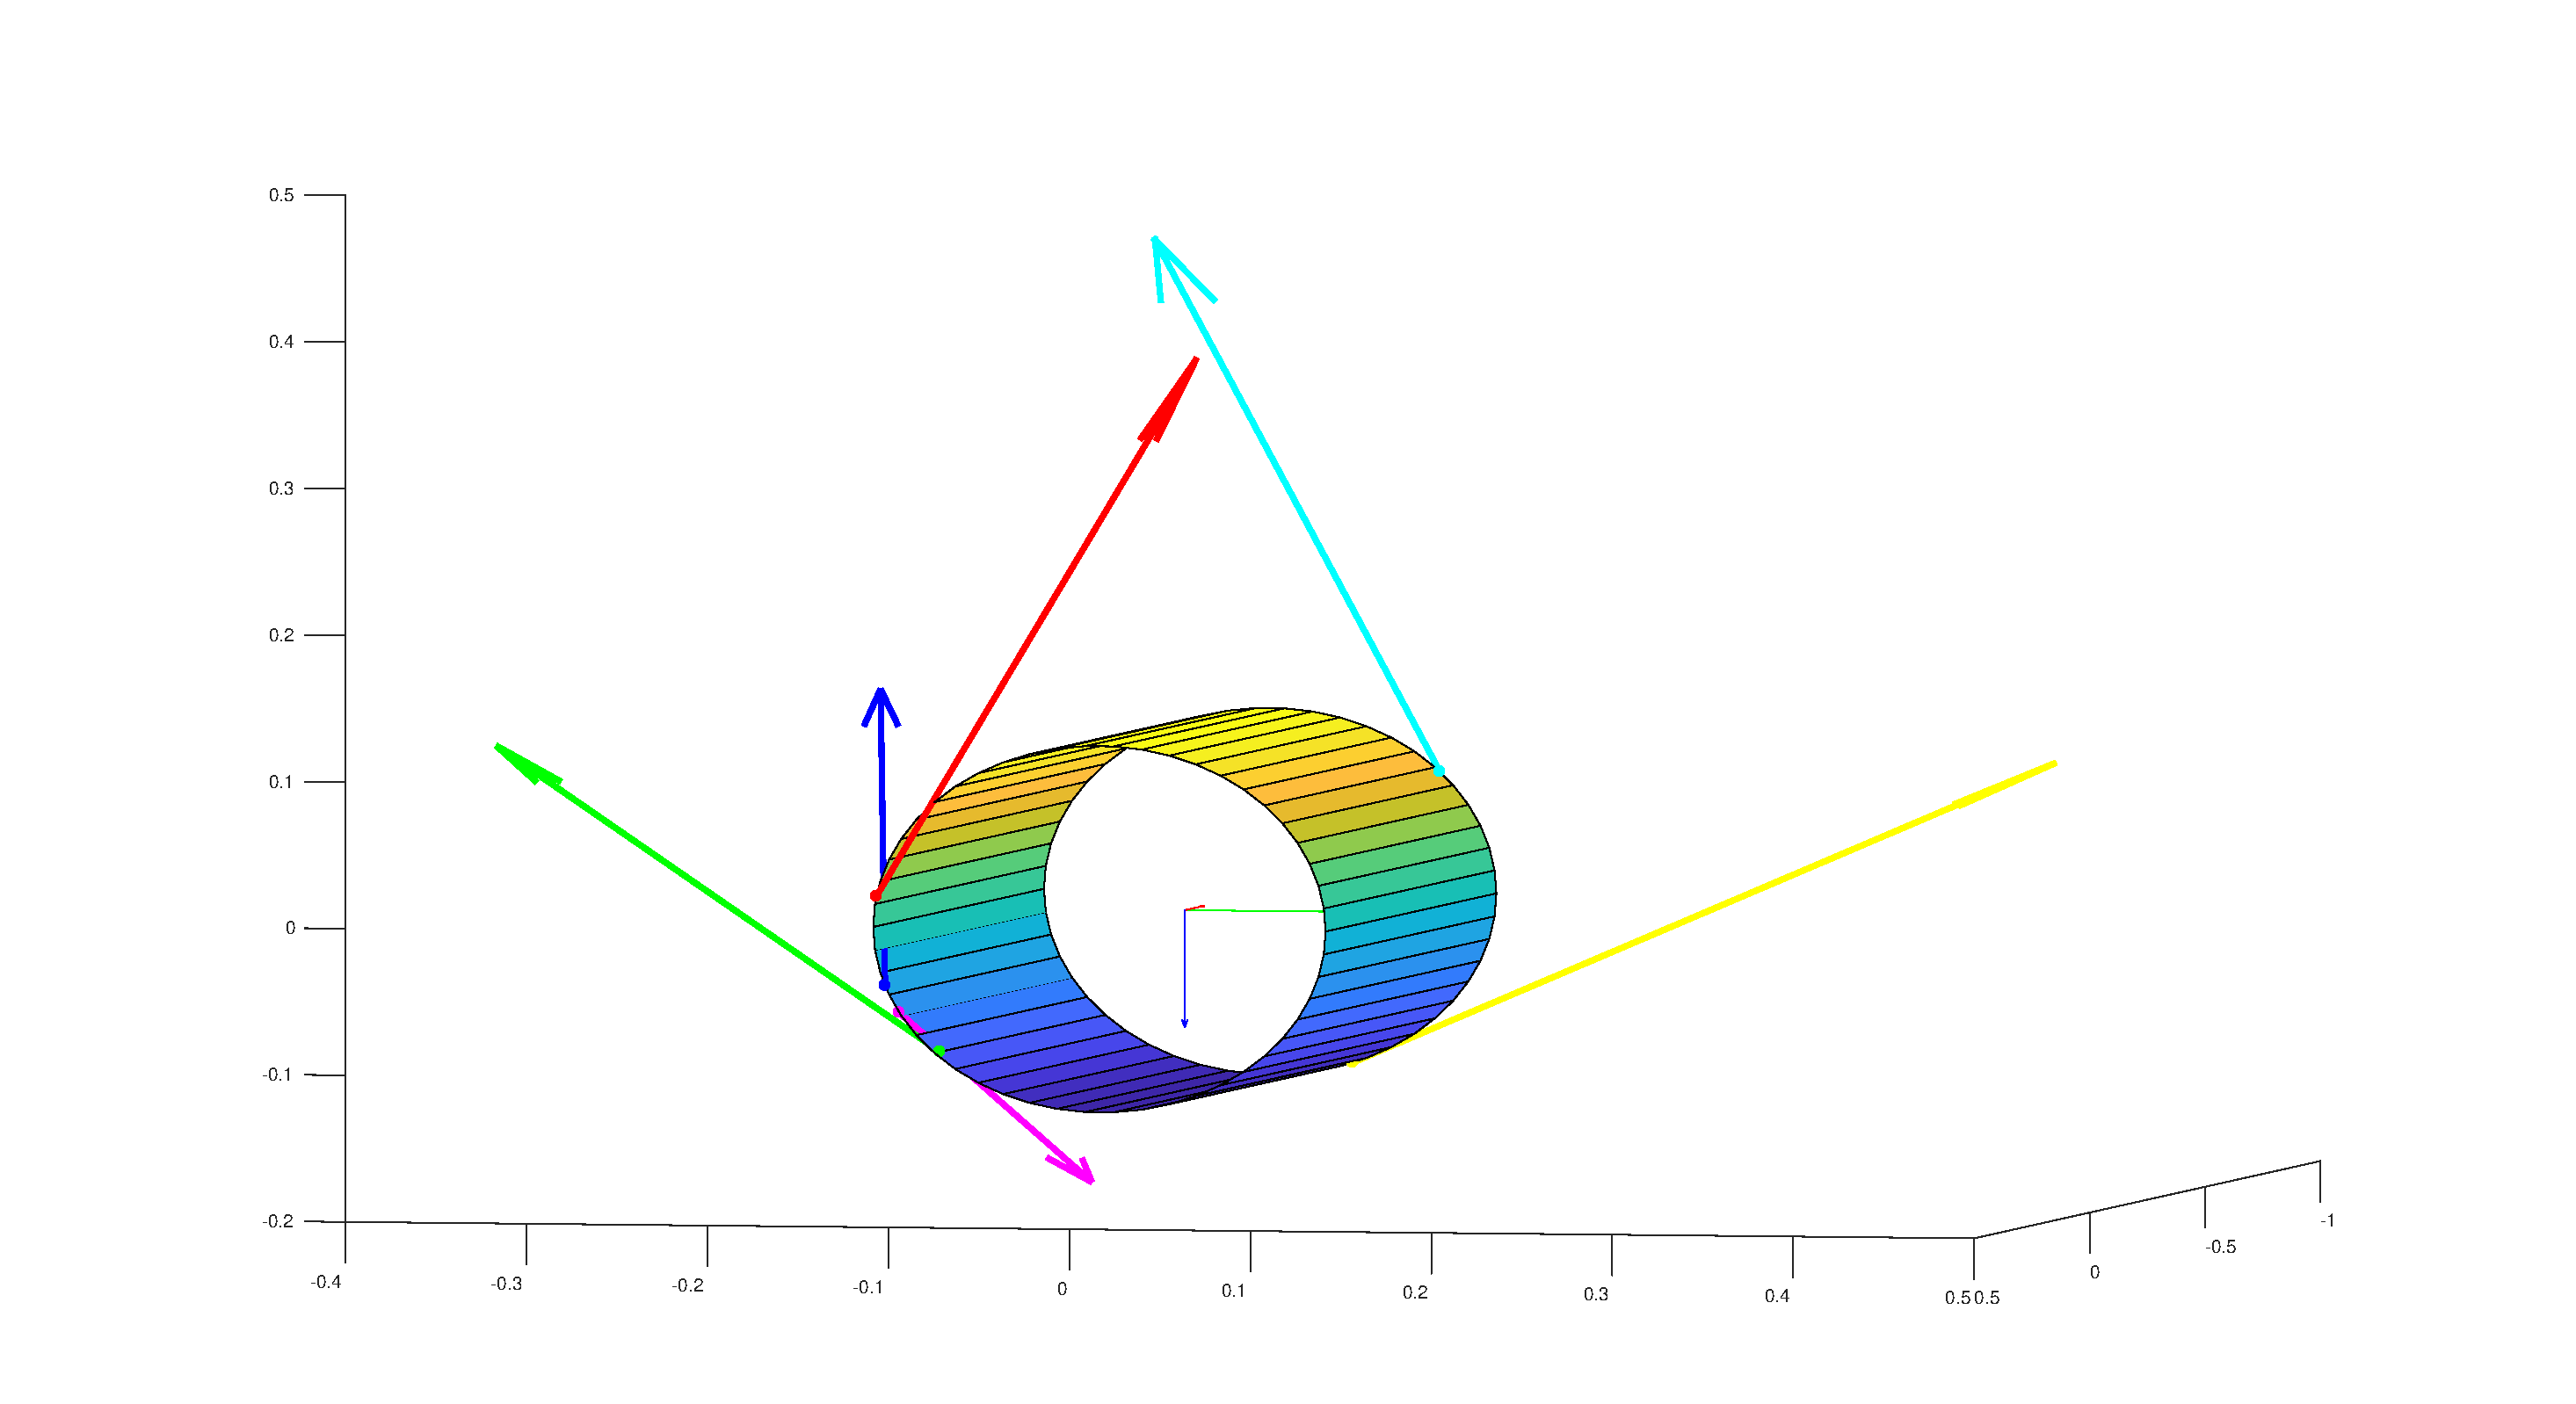
\includegraphics[width=0.9\textwidth]{GeoVisualFinThrusterT11.eps}
\caption{Visualization of optimization result (6 thrusters) perspective 1}	
\label{FIG:GeoVisualFinThrusterT11}
\end{figure}
\begin{figure}
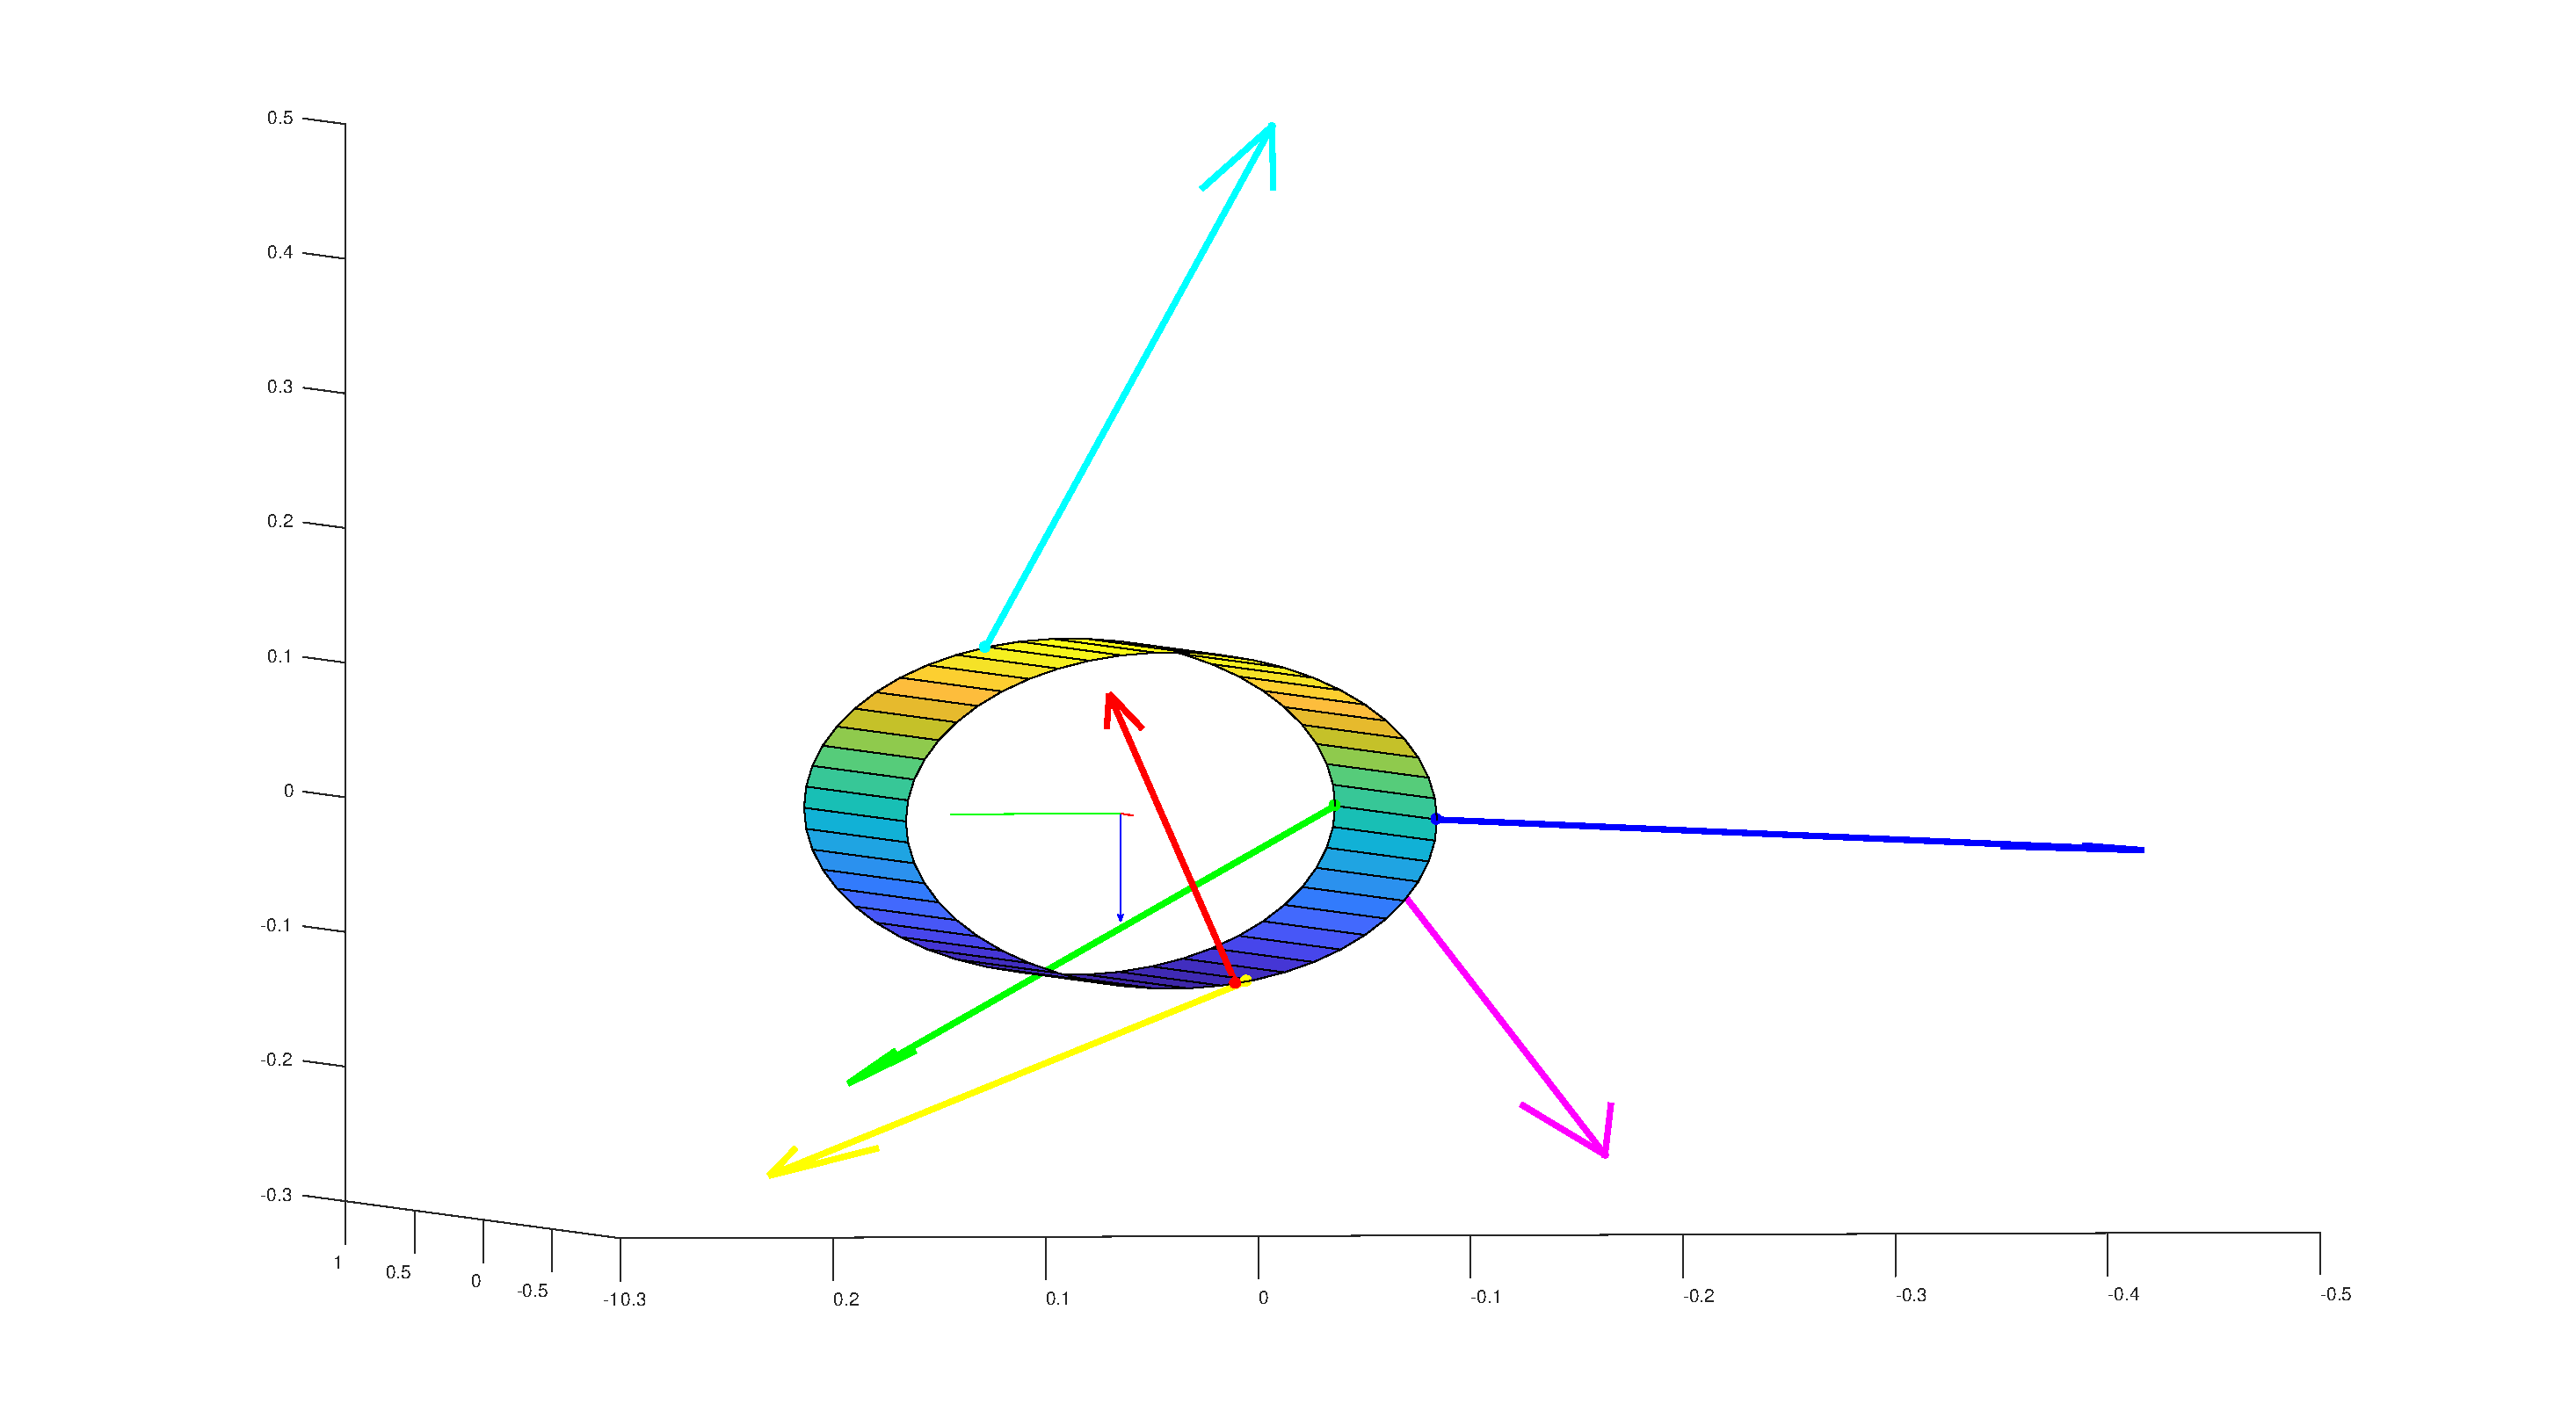
\includegraphics[width=\textwidth]{GeoVisualFinThrusterT12.eps}
\caption{Visualization of optimization result (6 thrusters) perspective 2}	
\label{FIG:GeoVisualFinThrusterT12}
\end{figure}

%%%%%%%%%%%%%%%%%%%%%%%%%%%%%%%%%%%%%%%%%%%%%%%%%%%%%%%%%%%%%%%%%%%%%%%%%%%%%%%%%
We set the value of $\epsilon$ according to the initial average norm of all trim trajectory error dynamics controllability matrices $\emph{\textbf{C}}_{E,av,init}=\dfrac{1}{7}\sum_{j=1}^{7}||\emph{\textbf{C}}_{E,j}^{1}||$, here we choose $\epsilon=0.001\emph{\textbf{C}}_{E,av,init}$. By using this $\epsilon$ value for breaking, the optimization algorithm will break only for 68 iterations, only one third of the specified maximal iterations ($k_{max}=200$). The norms of the error dynamics controllability matrices are in the order of $10^{9}$, as illustrated in Figure~\ref{FIG:ConNormT1}. They increase roughly in the first four iterations and fall down until the 18-th iteration. After that, the norm values do not change heavily and begin to converge slowly from the 50-th iteration.
\begin{figure}
\centering
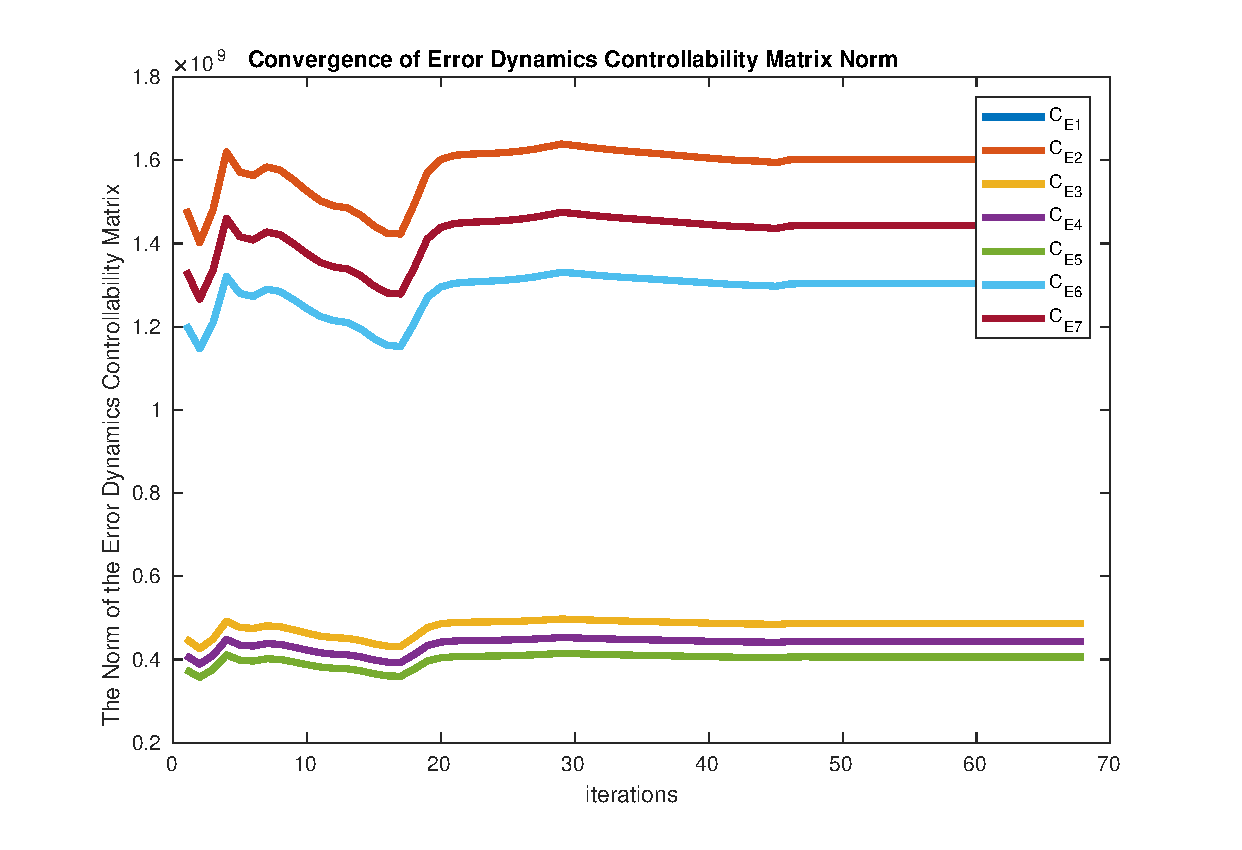
\includegraphics[width=0.75\textwidth]{ConNormT1.eps}
\caption{Convergence of error dynamics controllability matrix norm (6 thrusters)}	
\label{FIG:ConNormT1}
\end{figure}
The positions and orientations of the 6 thrusters are depicted in~\ref{FIG:ConPosInput2}. The positions and orientations of all 6 thrusters except for the thruster 2 direction vector $\vec{d}_{T,2}$ change obviously in the first 50 iterations and tend to converge from the 50-th iteration corresponding to the convergence of the controllability matrices norms. Only one direction vector's changing contributes to the norm negligibly, the optimization loop can still be broken. 

%%%%%%%%%%%%%%%%%%%%%%%%%%%%%%%%%%%%%%%%%%%%%%%%%%%%%%%%%%%%%%%%%%%%%%%%%%%%%%%%%
\begin{figure}
\centering
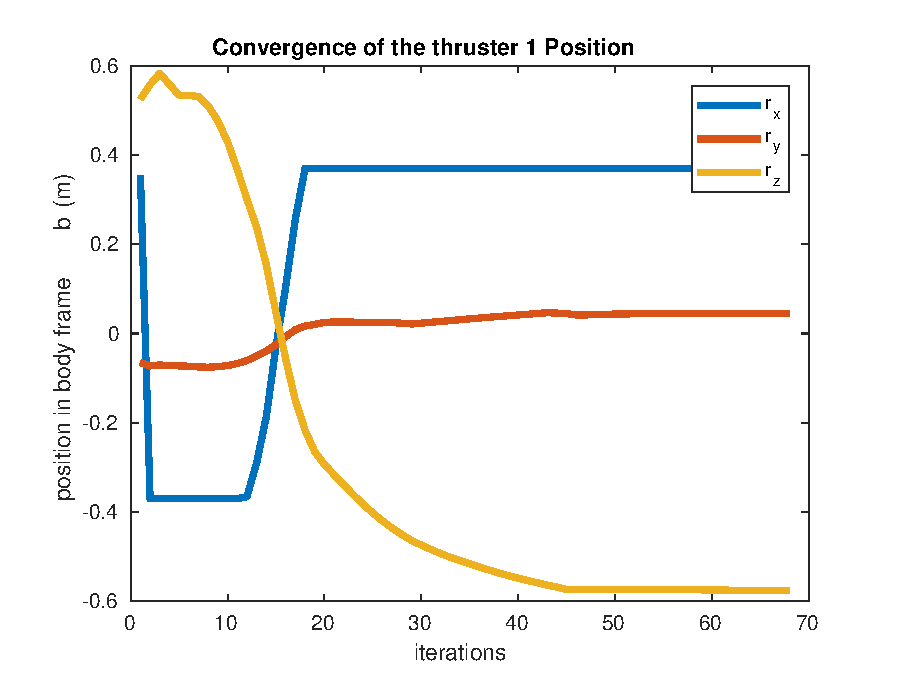
\includegraphics[width=0.45\textwidth]{ConThruster1PosT1.eps}
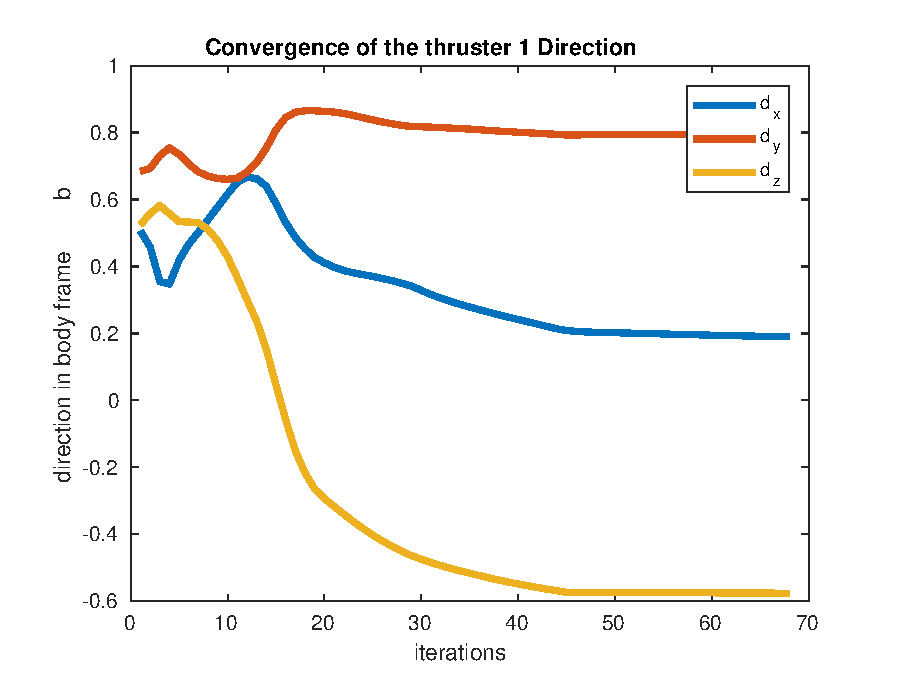
\includegraphics[width=0.45\textwidth]{ConThruster1DirT1.eps}
\caption{Convergence of position and direction of thruster 1 (6 thrusters)}	
\label{FIG:ConThrusterT11}
\end{figure}
\begin{figure}
\centering
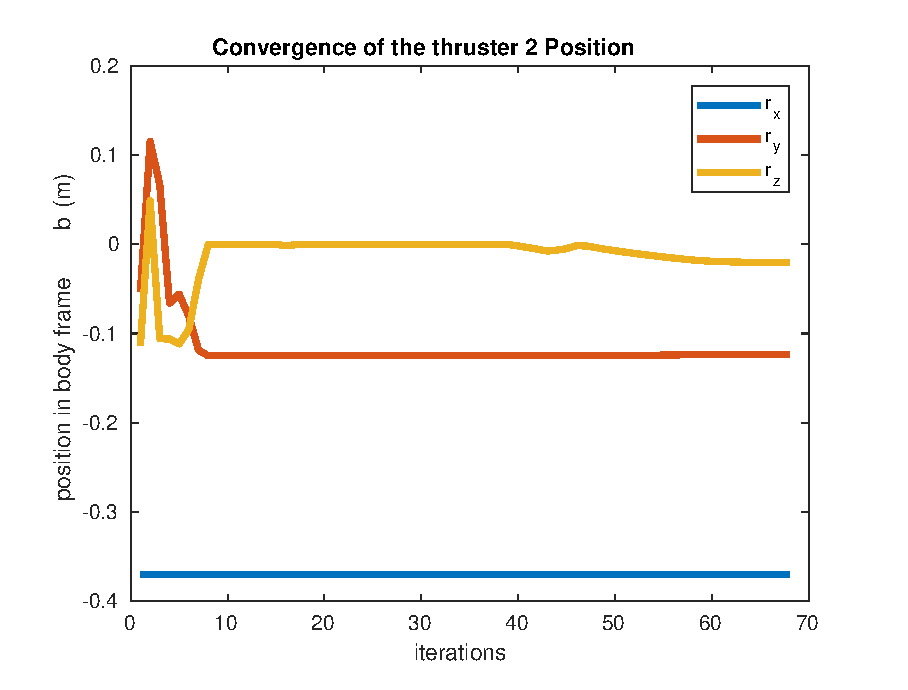
\includegraphics[width=0.45\textwidth]{ConThruster2PosT1.eps}
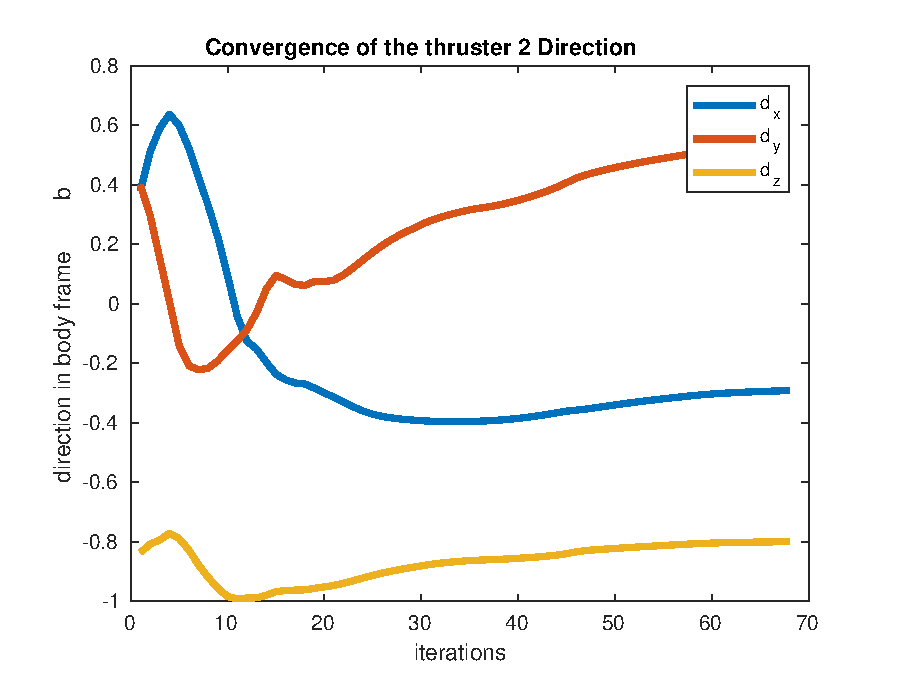
\includegraphics[width=0.45\textwidth]{ConThruster2DirT1.eps}
\caption{Convergence of position and direction of thruster 2 (6 thrusters)}	
\label{FIG:ConThrusterT21}
\end{figure}
\begin{figure}
\centering
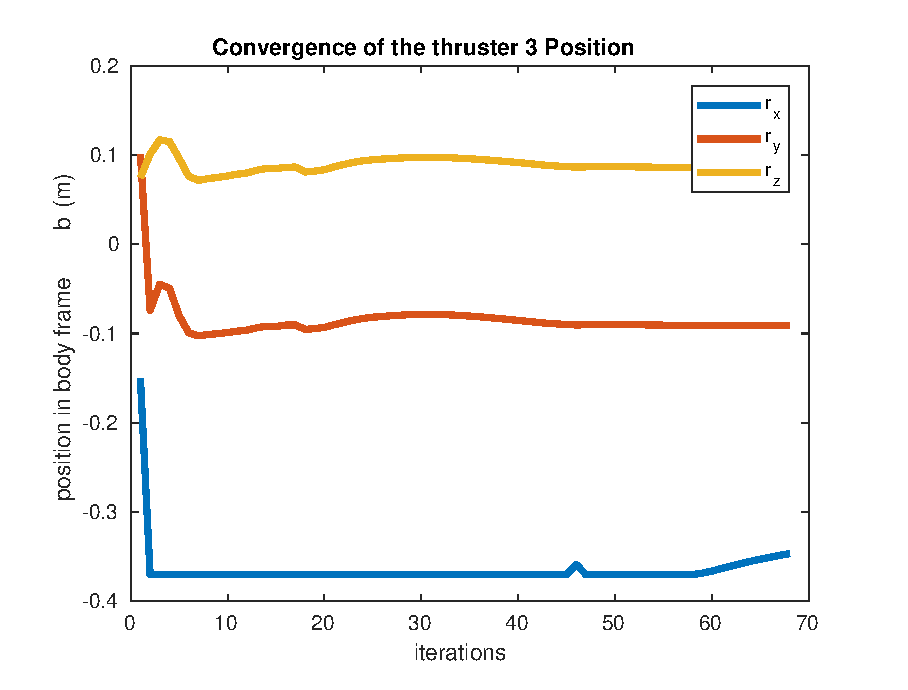
\includegraphics[width=0.45\textwidth]{ConThruster3PosT1.eps}
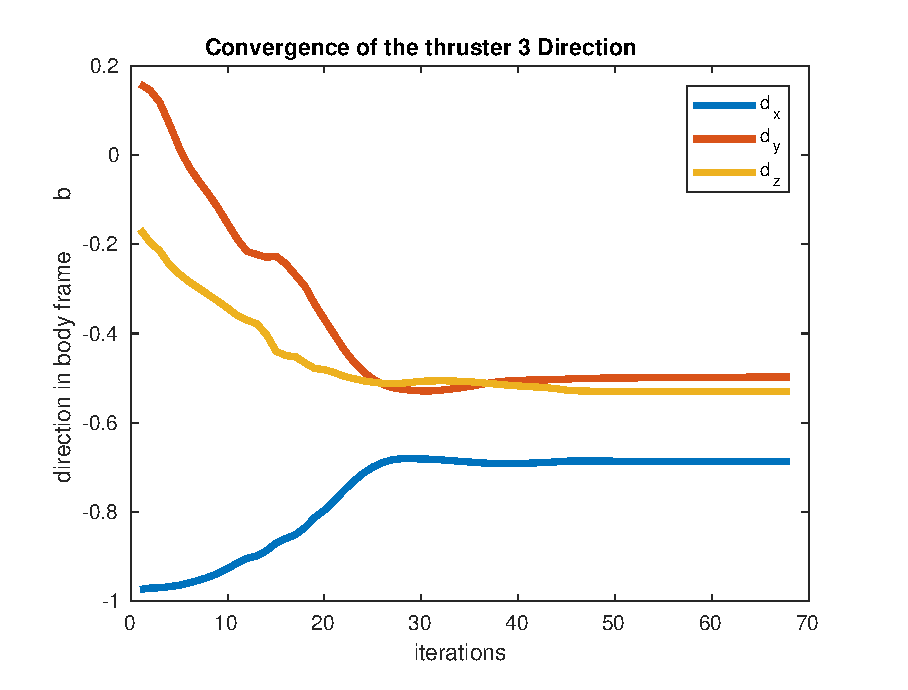
\includegraphics[width=0.45\textwidth]{ConThruster3DirT1.eps}
\caption{Convergence of position and direction of thruster 3 (6 thrusters)}	
\label{FIG:ConThrusterT31}
\end{figure}
\begin{figure}
\centering
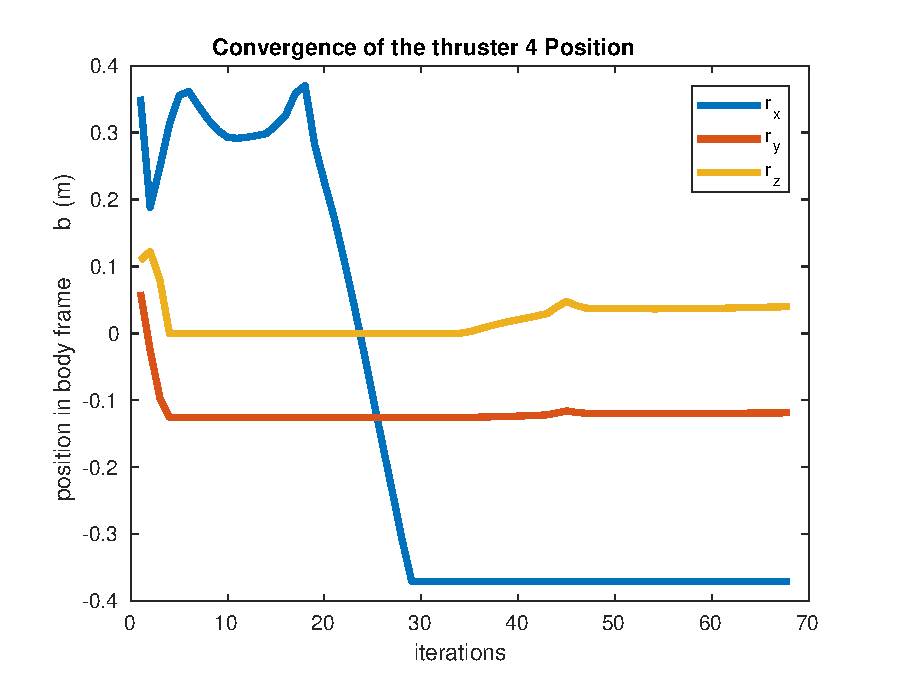
\includegraphics[width=0.45\textwidth]{ConThruster4PosT1.eps}
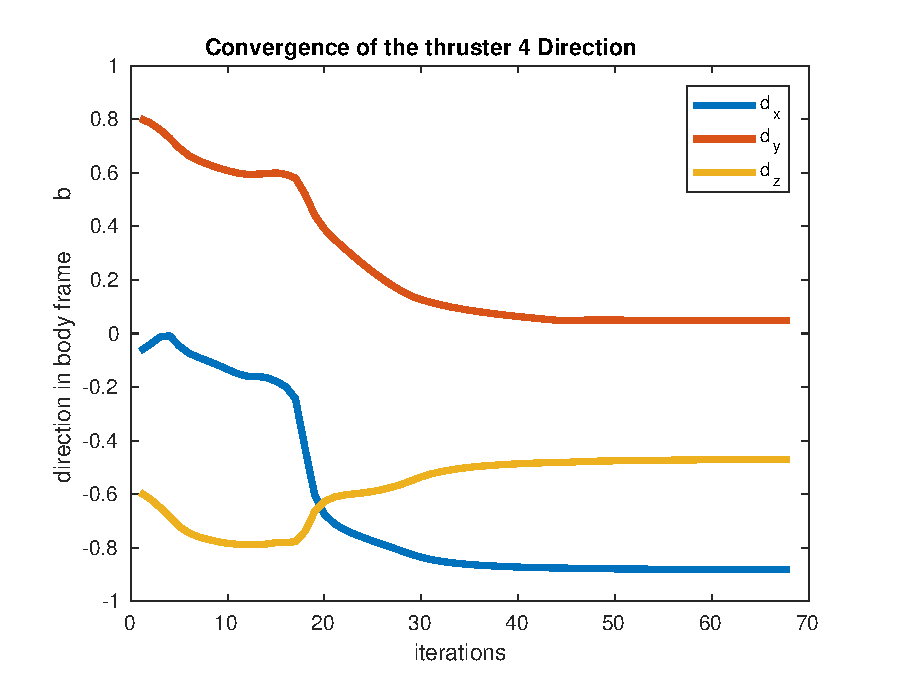
\includegraphics[width=0.45\textwidth]{ConThruster4DirT1.eps}
\caption{Convergence of position and direction of thruster 4 (6 thrusters)}	
\label{FIG:ConThrusterT41}
\end{figure}
\begin{figure}
\centering
\includegraphics[width=0.45\textwidth]{ConThruster5PosT1.eps}
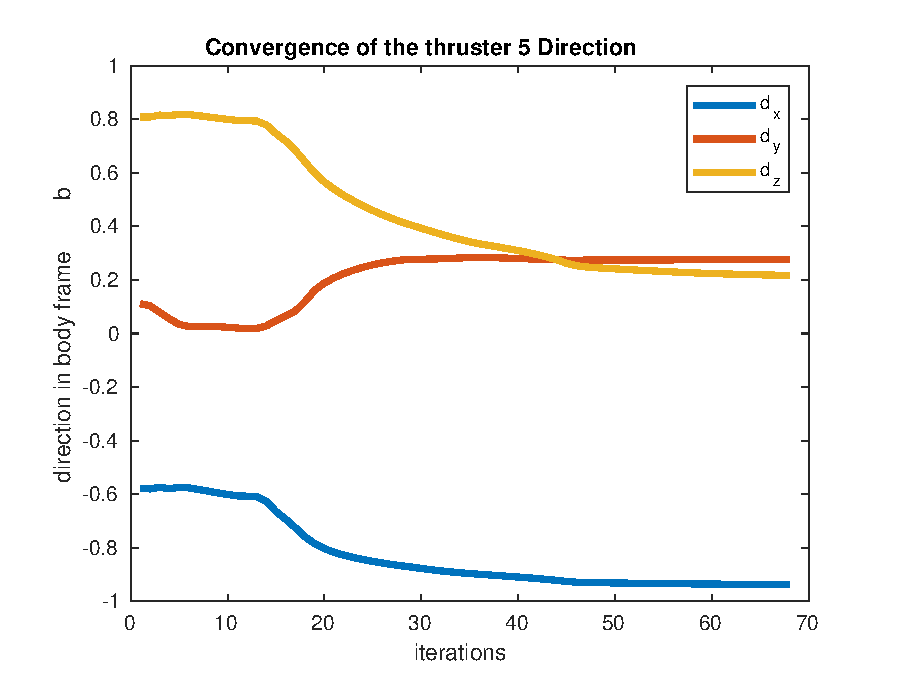
\includegraphics[width=0.45\textwidth]{ConThruster5DirT1.eps}
\caption{Convergence of position and direction of thruster 5 (6 thrusters)}	
\label{FIG:ConThrusterT51}
\end{figure}
\begin{figure}
\centering
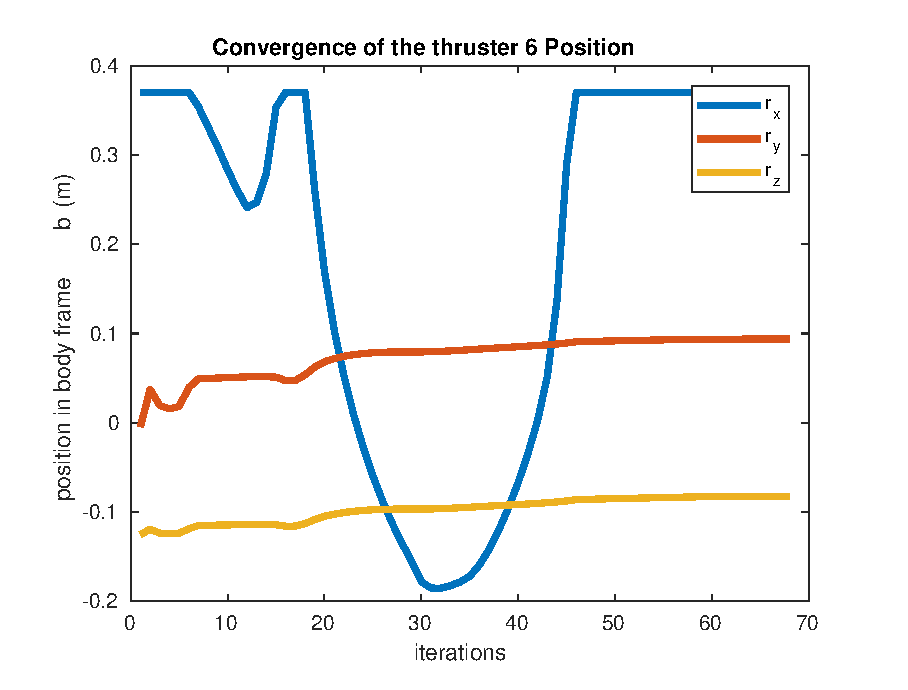
\includegraphics[width=0.45\textwidth]{ConThruster6PosT1.eps}
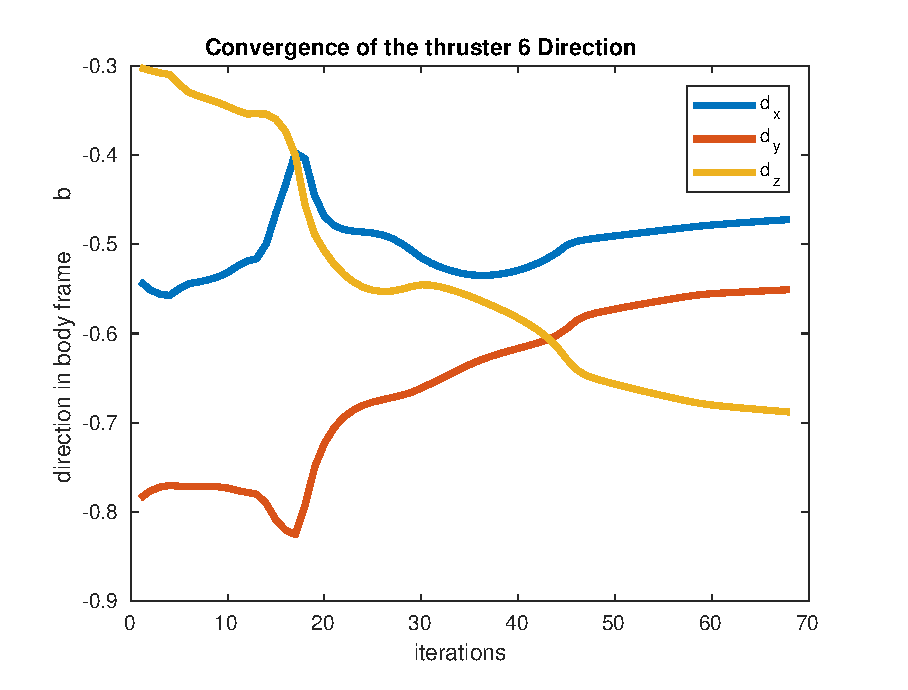
\includegraphics[width=0.45\textwidth]{ConThruster6DirT1.eps}
\caption{Convergence of position and direction of thruster 6 (6 thrusters)}	
\label{FIG:ConThrusterT61}
\end{figure}

Recall that we have three optimization steps: control input optimization, position optimization and orientation optimization. As depicted in Figure~\ref{FIG:ConInputPosT1}, the control input objective function (~\ref{EQ:OPTInput}) value $fval_{input}$ increases from 210 to 380 and then decreases significantly to 50 at the iteration 30. After that, it falls down slightly until the last iteration. The convergence value of $fval_{input}$ is merely one fifths of the initial objective value, namely 40. The position optimization objective value $fval_{pos}$ starts also approximately from 110 and decreases to 10 in 68 optimization loops.

\begin{figure}
\center
\includegraphics[width=0.49\textwidth]{ConInputT1.eps}
\includegraphics[width=0.49\textwidth]{ConPosT1.eps}
\caption{Value of objective functions (6 thrusters)}	
\label{FIG:ConInputPosT1}
\end{figure}
\newpage
We build the switched LQR controller using the state cost and input cost matrices from Table~\ref{table:QParameters} and~\ref{table:RParameters for 6 thrusters}. 
Under the current configuration, we want the robot to track the specified 7 trim trajectories in~\ref{table:TrimValues}. As illustrated in~\ref{FIG:TrackUnsatT1}, the robot can realize perfect tracking without actuator constraint. When we add the actuator saturation, as depicted in Figure~\ref{FIG:TrackSatT1}, the robot is able to keep the trim paths roughly.
  
\begin{table}
\centering
\small
\caption{State cost matrices }
\begin{tabular}{| c | c | c | p{0.5cm} |}
\hline
Index&$\mathcal{Q}_{E}$\\ \hline
1&diag([1000,1000,1000,300,300,300,1,1,1,1,1,1]) \\ \hline
2&diag([1000,1000,1000,300,300,300,1,1,1,1,1,1]) \\ \hline
3&diag([1000,1000,1000,300,300,300,1,1,1,1,1,1])\\ \hline
4&diag([1000,1000,1000,1,1,1,1,1,1,1,1,1]) \\ \hline
5&diag([1000,1000,1000,300,300,300,1,1,1,1,1,1])\\ \hline
6&diag([1000,1000,1000,300,300,300,1,1,1,1,1,1])\\ \hline
7&diag([1000,1000,1000,300,300,300,1,1,1,1,1,1]) \\ \hline
\end{tabular}
\label{table:QParameters}
\end{table} 
\begin{table}
\centering
\small
\caption{Input cost matrices for 6 thrusters}
\begin{tabular}{| c | c | c | c | p{0.5cm} |}
\hline
Index&$\mathcal{R}_{E}$ \\ \hline
1&diag([0.001,0.001,0.001,0.001,0.001,0.001])\\ \hline
2&diag[0.001,0.001,0.001,0.001,0.001,0.001] \\ \hline
3&diag([0.0001,0.0001,0.0001,0.0001,0.0001,0.0001])\\ \hline
4&diag([0.0001,0.0001,0.0001,0.0001,0.0001,0.0001]) \\ \hline
5&diag([0.0001,0.0001,0.0001,0.0001,0.0001,0.0001])\\ \hline
6&diag([0.0001,0.0001,0.0001,0.0001,0.0001,0.0001])\\ \hline
7&diag([0.001,0.001,0.001,0.001,0.001,0.001]) \\ \hline
\end{tabular}
\label{table:RParameters for 6 thrusters}
\end{table} 

\begin{figure}
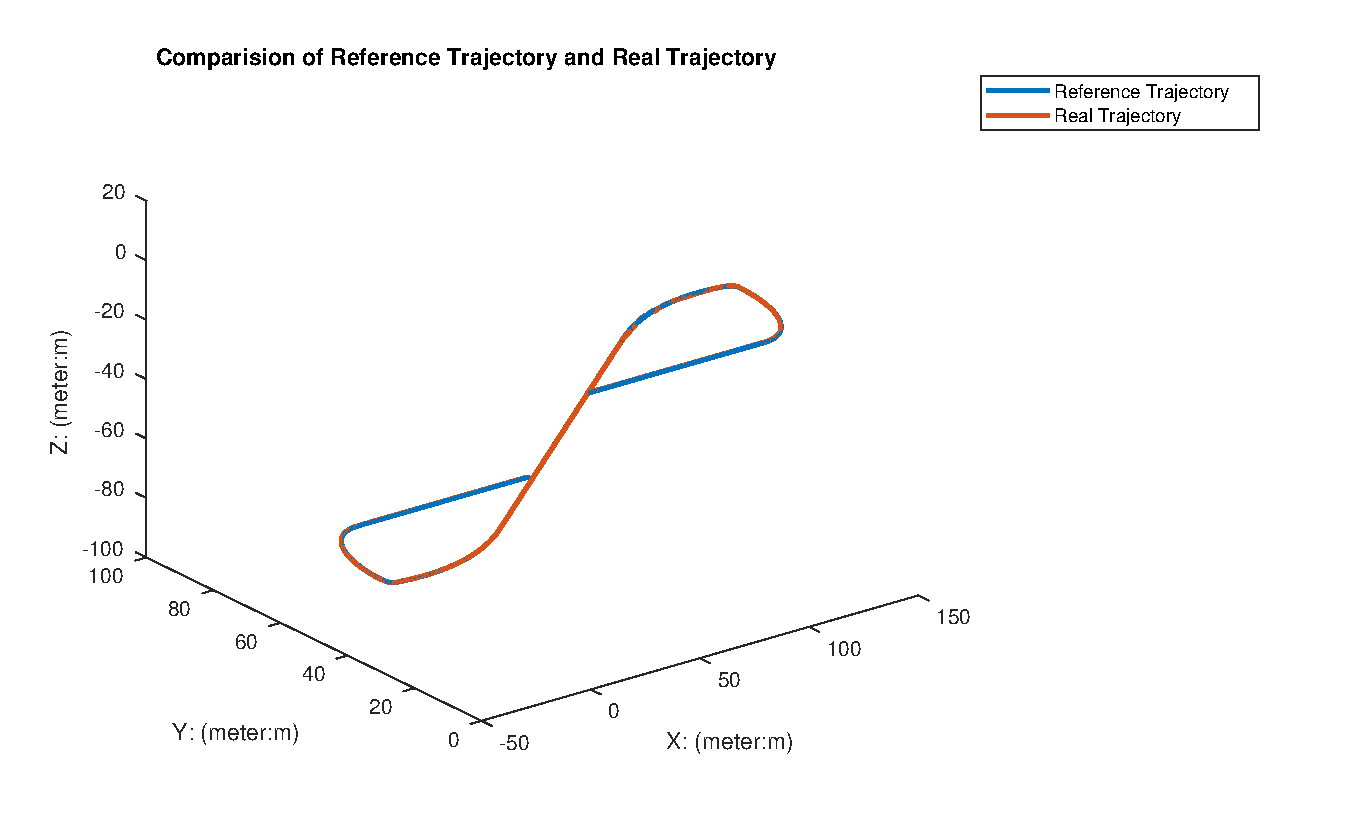
\includegraphics[width=\textwidth]{TrackUnsatT1.eps}
\caption{Comparison of desired trajectory and real trajectory (6 thrusters, no actuator saturation)}	
\label{FIG:TrackUnsatT1}
\end{figure}
\begin{figure}
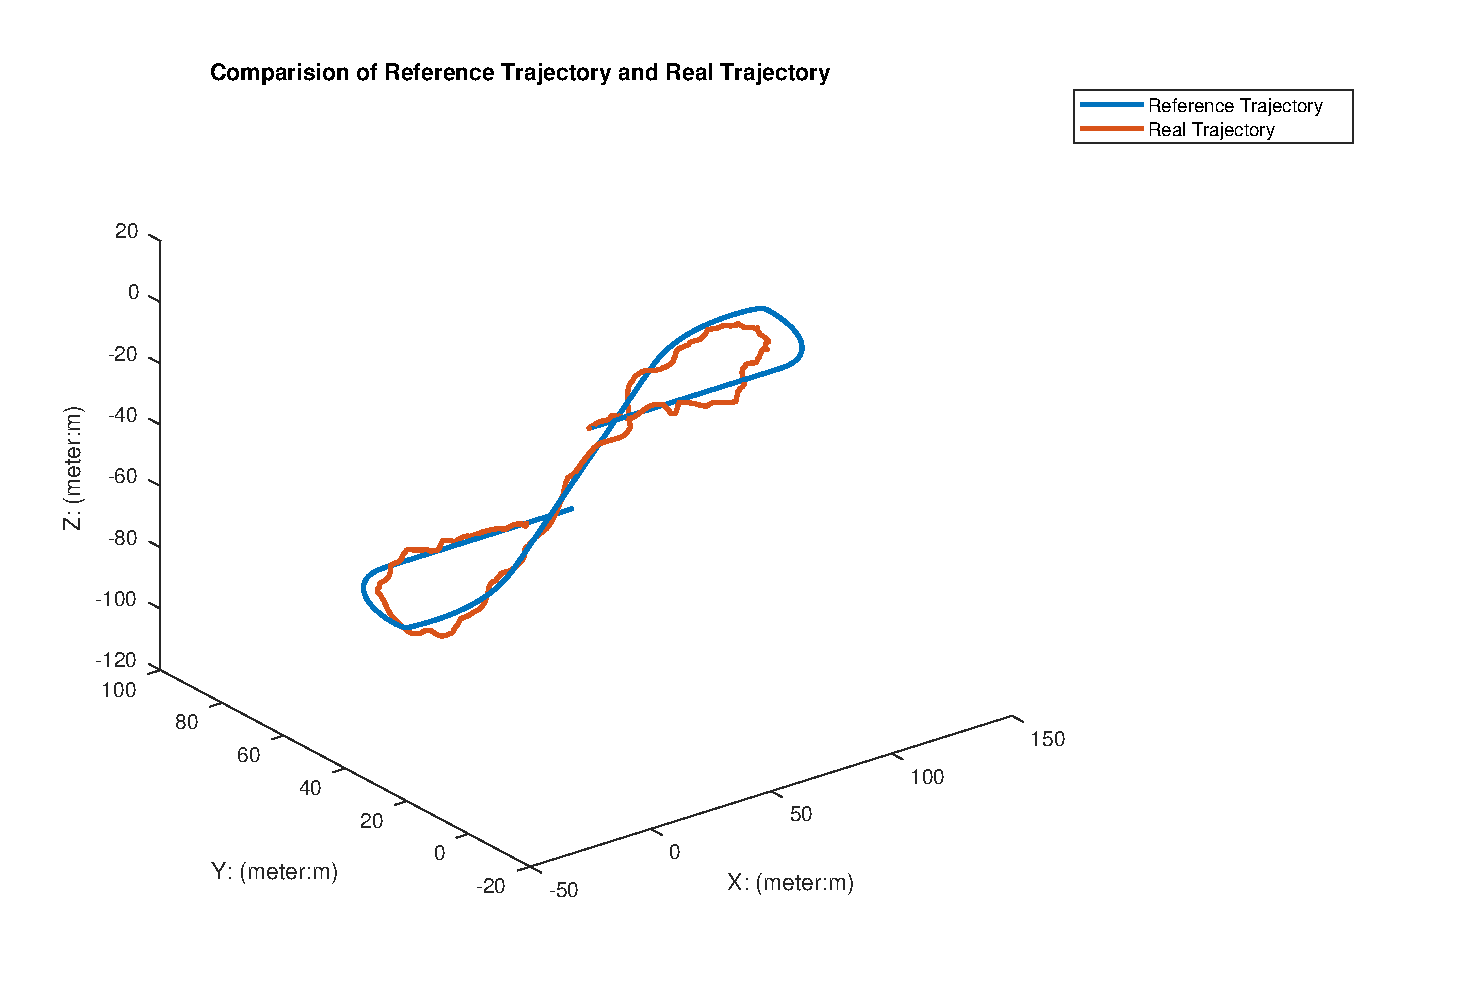
\includegraphics[width=\textwidth]{TrackSatT1.eps}
\caption{Comparison of desired trajectory and real trajectory (6 thrusters, with actuator saturation)}	
\label{FIG:TrackSatT1}
\end{figure}

\section{Training and Test for Thrusters}
As mentioned before, in this session,  we use a trim trajectory segment as training data for the optimal geometric parameters for the 6 thrusters and another trim trajectory segment for validating. The trim specifications are listed in Table~\ref{table:TrimValuesTrainTest}. The train trim trajectory possess a double trim speed ($||\vec{v}_{\mathcal{T}}||=2$ m/s) than the test trim segment ($||\vec{v}_{\mathcal{T}}||=1$ m/s). The yaw rate direction of the train trim is opposed to that of the test trajectory with nearly triple magnitude. The motion path angle $\gamma_{\mathcal{T}}$ of the train trim segment is a little smaller than that of the validation trim segment.

\begin{table}[h]
\centering
\caption{Trim Trajectory Specifications}
\begin{tabular}{| c | c | c | c | p{2cm} |}
\hline
Trim Trajectory Property&Time(s)&$||\vec{v}_{\mathcal{T}}||$ (m/s)&$\dot{\psi}_{\mathcal{T}}$ (rad/s)&$\gamma_{\mathcal{T}}$ (rad)\\ \hline
Train Trajectory&0-100&2&0.1&0.5\\ \hline
Test Trajectory&100-125&1&-0.35&0.6 \\ \hline
\end{tabular}
\label{table:TrimValuesTrainTest}
\end{table} 

General speaking, the train trim trajectory segment is more difficult to be tracked by the robot than the validation trim trajectory segment.     
 
\begin{figure}[h]
\center
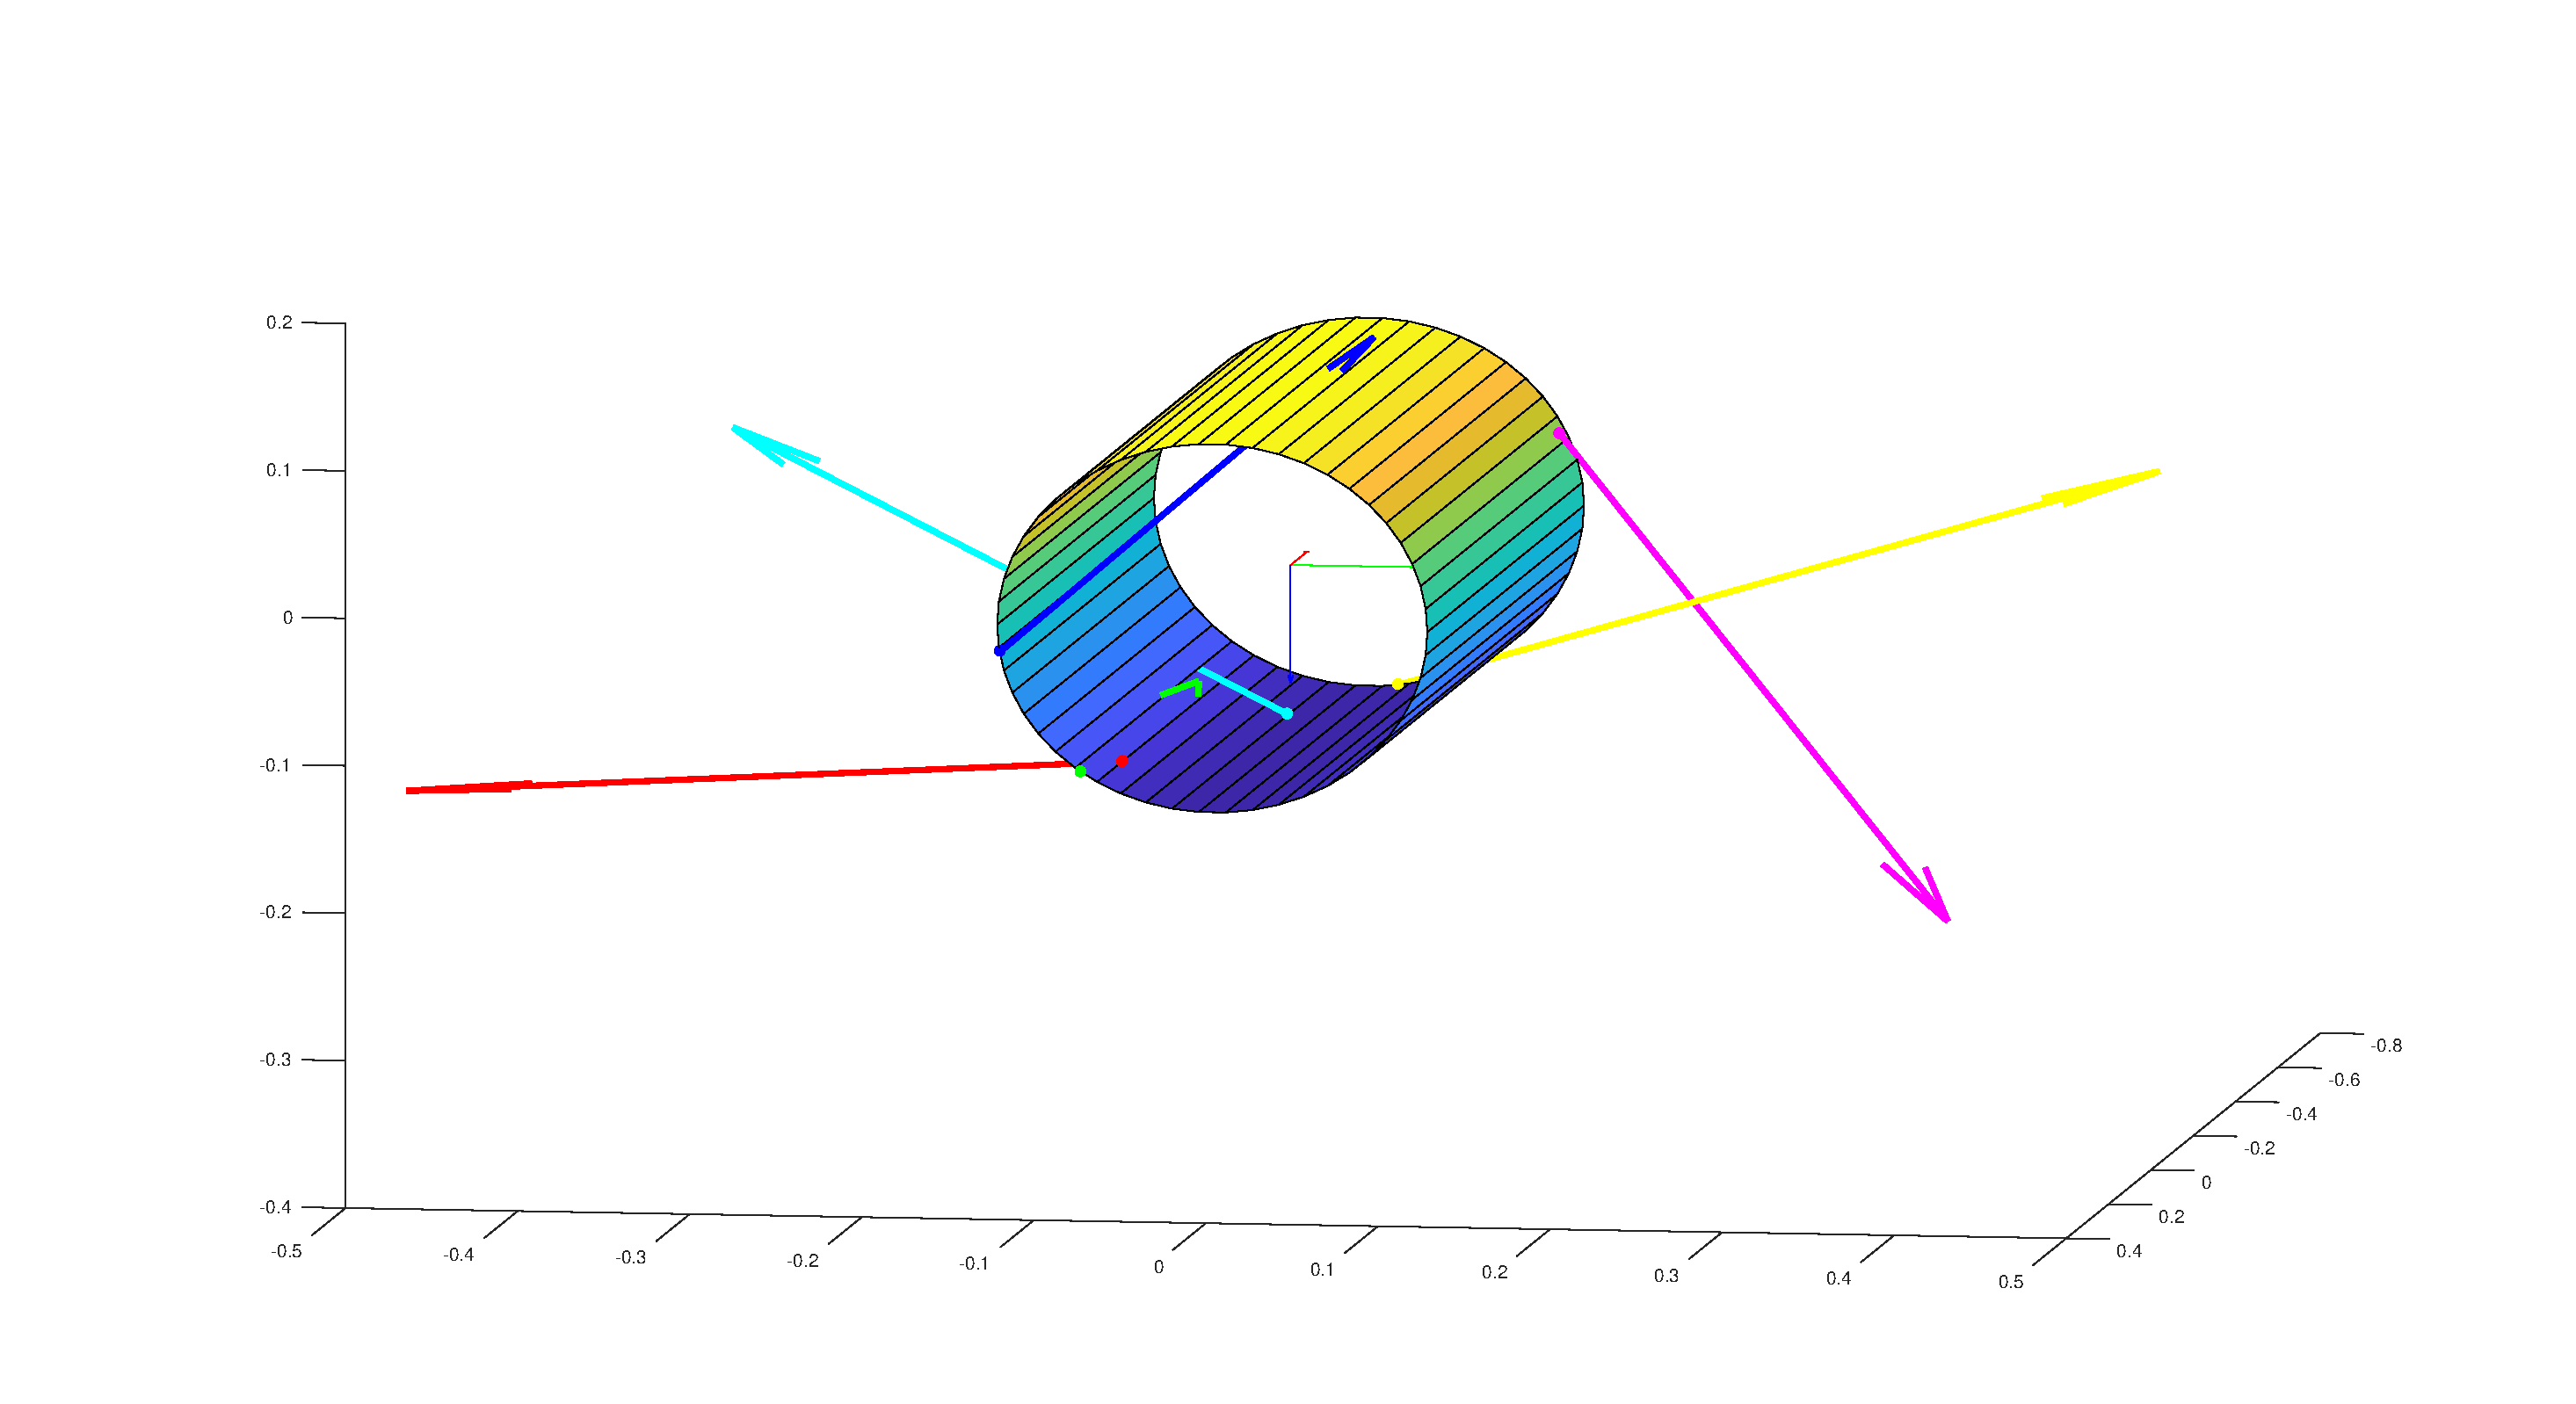
\includegraphics[width=0.9\textwidth]{GeoVisualFinThrusterTT1.eps}
\caption{Visualization of optimization result (6 thrusters, train and test) perspective 1}	
\label{FIG:GeoVisualFinThrusterTT1}
\end{figure}
\begin{figure}[h]
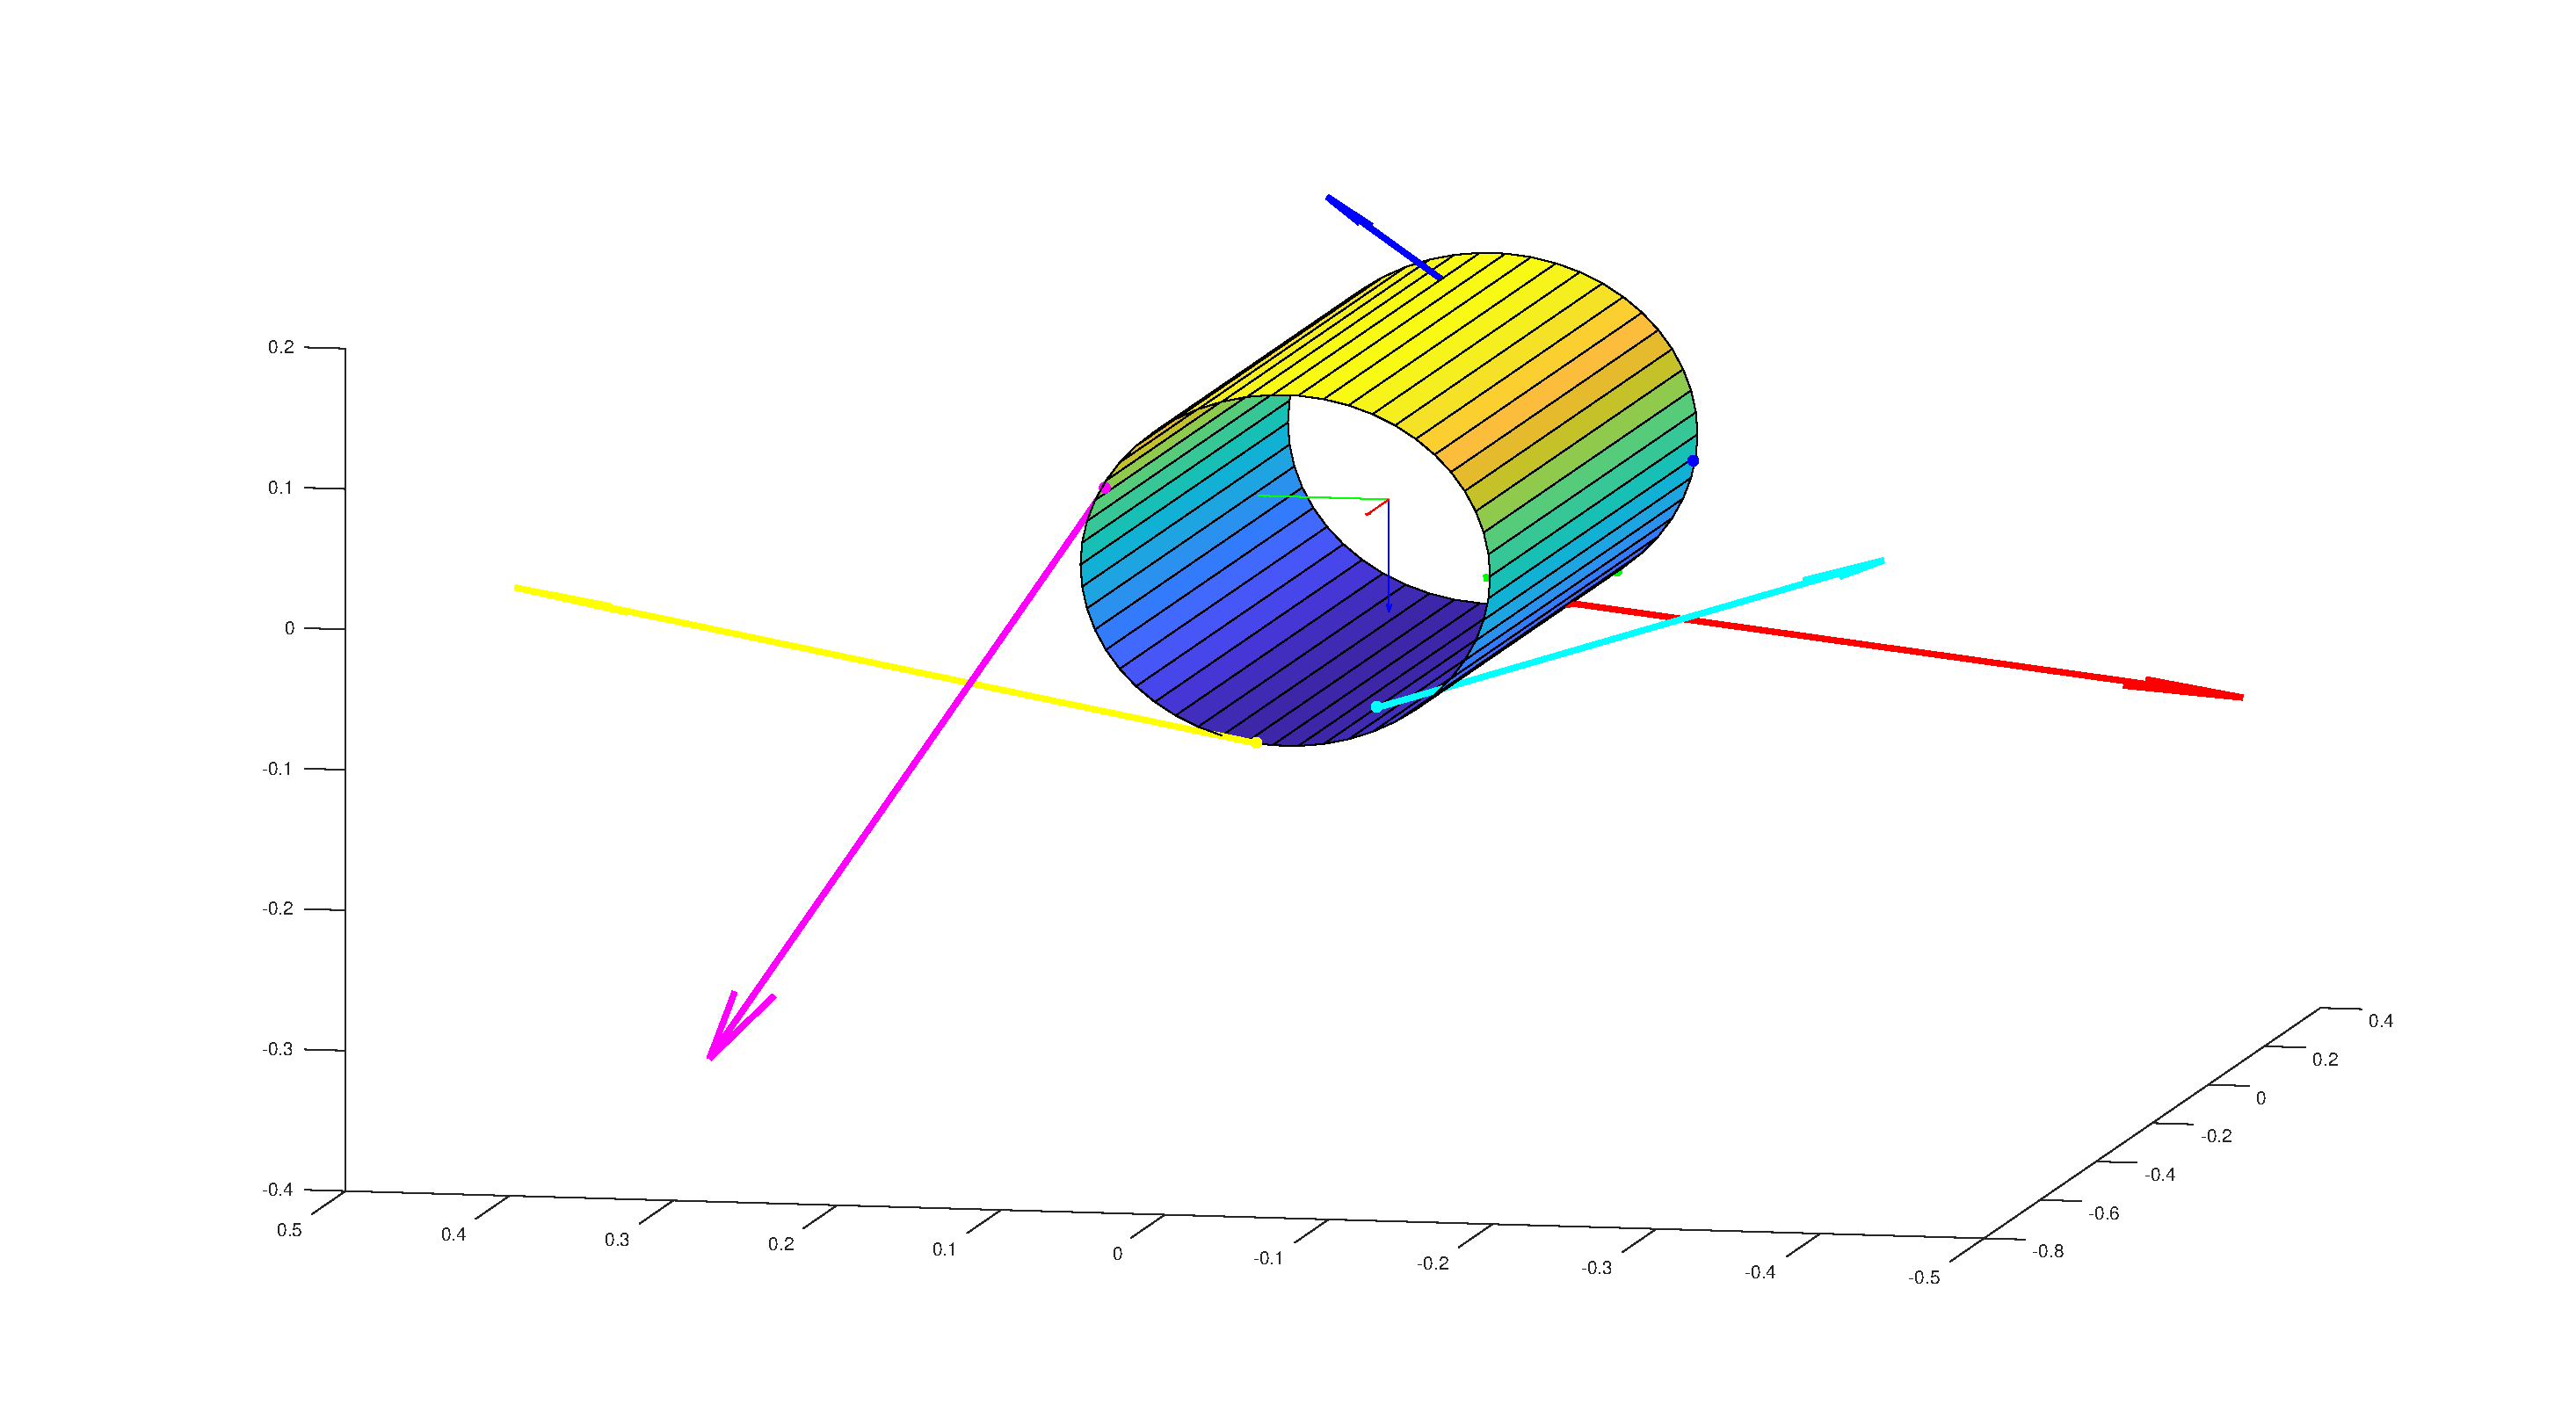
\includegraphics[width=\textwidth]{GeoVisualFinThrusterTT2.eps}
\caption{Visualization of optimization result (6 thrusters, train and test) perspective 2}	
\label{FIG:GeoVisualFinThrusterTT2}
\end{figure}
\newpage  
Since only one trim trajectory segment need to be tracked, the calculation amount is much less than the case of seven trim trajectories in the previous section. From Figures~\ref{FIG:ConThruster1TT},~\ref{FIG:ConThruster2TT}, \ref{FIG:ConThruster3TT},~\ref{FIG:ConThruster3TT},~\ref{FIG:ConThruster4TT},
~\ref{FIG:ConThruster5TT}, ~\ref{FIG:ConThruster6TT}, we can see that the positions and orientations of the 6 thrusters converge within only 4 iterations, which corresponds to the variations of the controllability matrix norm $\emph{\textbf{C}}_{E,1}$ illustrated in Figure~\ref{FIG:ConNormTT}.
\begin{figure}[h]
\centering
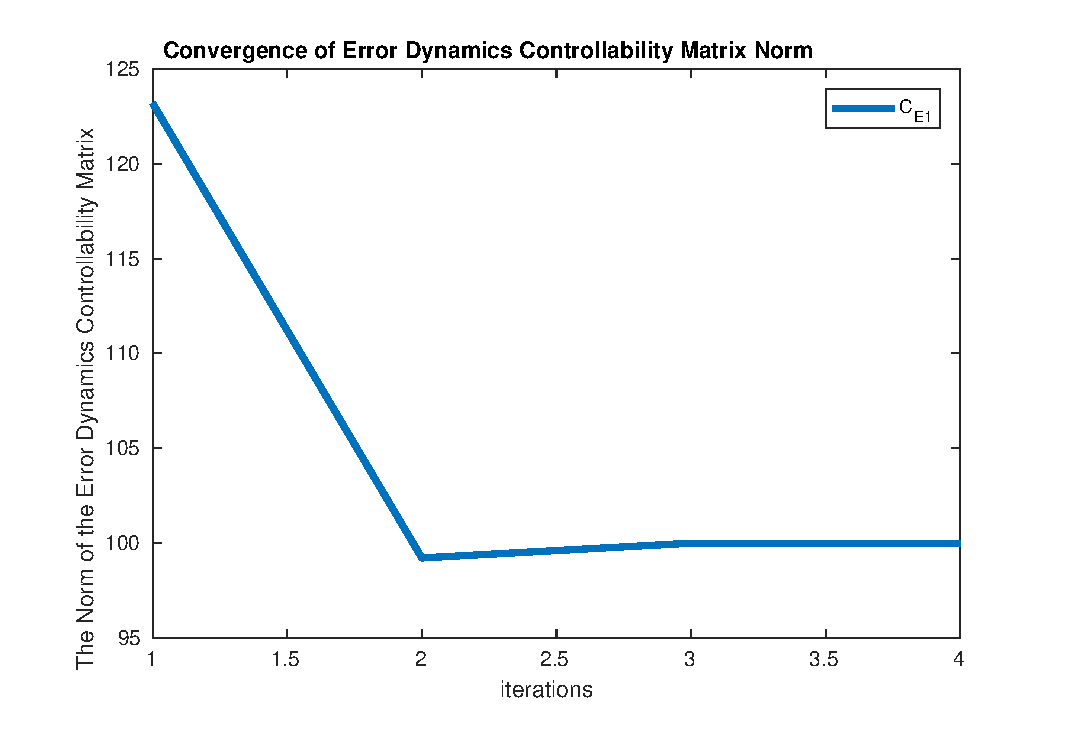
\includegraphics[width=0.7\textwidth]{ConNormTT.eps}
\caption{Convergence of error dynamics controllability matrix norm (6 thrusters, train and test)}	
\label{FIG:ConNormTT}
\end{figure}

%%%%%%%%%%%%%%%%%%%%%%%%%%%%%%%%%%%%%%%%%%%%%%%%%%%%%%%%%%%%%%%%%%%%%%%%%%%%%%%%%
\begin{figure}
\centering
\includegraphics[width=0.45\textwidth]{ConThruster1PosTT.eps}
\includegraphics[width=0.45\textwidth]{ConThruster1DirTT.eps}
\caption{Convergence of position and direction of thruster 1 (6 thrusters, train and test)}	
\label{FIG:ConThruster1TT}
\end{figure}
\begin{figure}
\centering
\includegraphics[width=0.45\textwidth]{ConThruster2PosTT.eps}
\includegraphics[width=0.45\textwidth]{ConThruster2DirTT.eps}
\caption{Convergence of position and direction of thruster 2 (6 thrusters, train and test)}	
\label{FIG:ConThruster2TT}
\end{figure}
\begin{figure}
\centering
\includegraphics[width=0.45\textwidth]{ConThruster3PosTT.eps}
\includegraphics[width=0.45\textwidth]{ConThruster3DirTT.eps}
\caption{Convergence of position and direction of thruster 3 (6 thrusters, train and test)}	
\label{FIG:ConThruster3TT}
\end{figure}
\begin{figure}
\centering
\includegraphics[width=0.45\textwidth]{ConThruster4PosTT.eps}
\includegraphics[width=0.45\textwidth]{ConThruster4DirTT.eps}
\caption{Convergence of position and direction of thruster 4 (6 thrusters, train and test)}	
\label{FIG:ConThruster4TT}
\end{figure}
\begin{figure}
\centering
\includegraphics[width=0.45\textwidth]{ConThruster5PosTT.eps}
\includegraphics[width=0.45\textwidth]{ConThruster5DirTT.eps}
\caption{Convergence of position and direction of thruster 5 (6 thrusters, train and test)}	
\label{FIG:ConThruster5TT}
\end{figure}
\begin{figure}
\centering
\includegraphics[width=0.45\textwidth]{ConThruster6PosTT.eps}
\includegraphics[width=0.45\textwidth]{ConThruster6DirTT.eps}
\caption{Convergence of position and direction of thruster 6 (6 thrusters, train and test)}	
\label{FIG:ConThruster6TT}
\end{figure}

\begin{figure}
\center
\includegraphics[width=0.49\textwidth]{ConInputTT.eps}
\includegraphics[width=0.49\textwidth]{ConPosTT.eps}
\caption{Value of objective function (6 thrusters, train and test)}	
\label{FIG:ConInputPosTT}
\end{figure}

\newpage
It is notable that the control input optimization error $fval_{input}$ and the position optimization error $fval_{pos}$ can be minimized to zero, which is not achievable for optimization in terms of seven trim trajectories. It is easy to find a actuator geometric configuration so that they can generate the desired trim input $\vec{\tau}_{\mathcal{T}}$ under saturation constraints for just one trim trajectory. However, when the desired trim trajectory segments increase to seven, 
a geometric configuration that is able to generate the desired seven trim generalized forces $\vec{\tau}_{d,\mathcal{T}_{1}}, \cdots, \vec{\tau}_{d,\mathcal{T}_{7}}$ under consideration of the actuator capability could not be found by our optimization algorithm.





\newpage

As illustrated in~\ref{FIG:TrackUnsatTT}, the trained robot from the first trim trajectory segment track both trim paths perfectly when the capability of the thrusters are not taken into consideration. The Figure~\ref{FIG:TrackSatTT} depicts the tracking performance when we specify the maximal and minimal thrust of the thrusters as $[-35,40]$ N. The tracking deviation from the desired train trim trajectory is bigger than that from the test trim trajectory due to its higher trim speed and yaw rate.

\begin{figure}
\centering
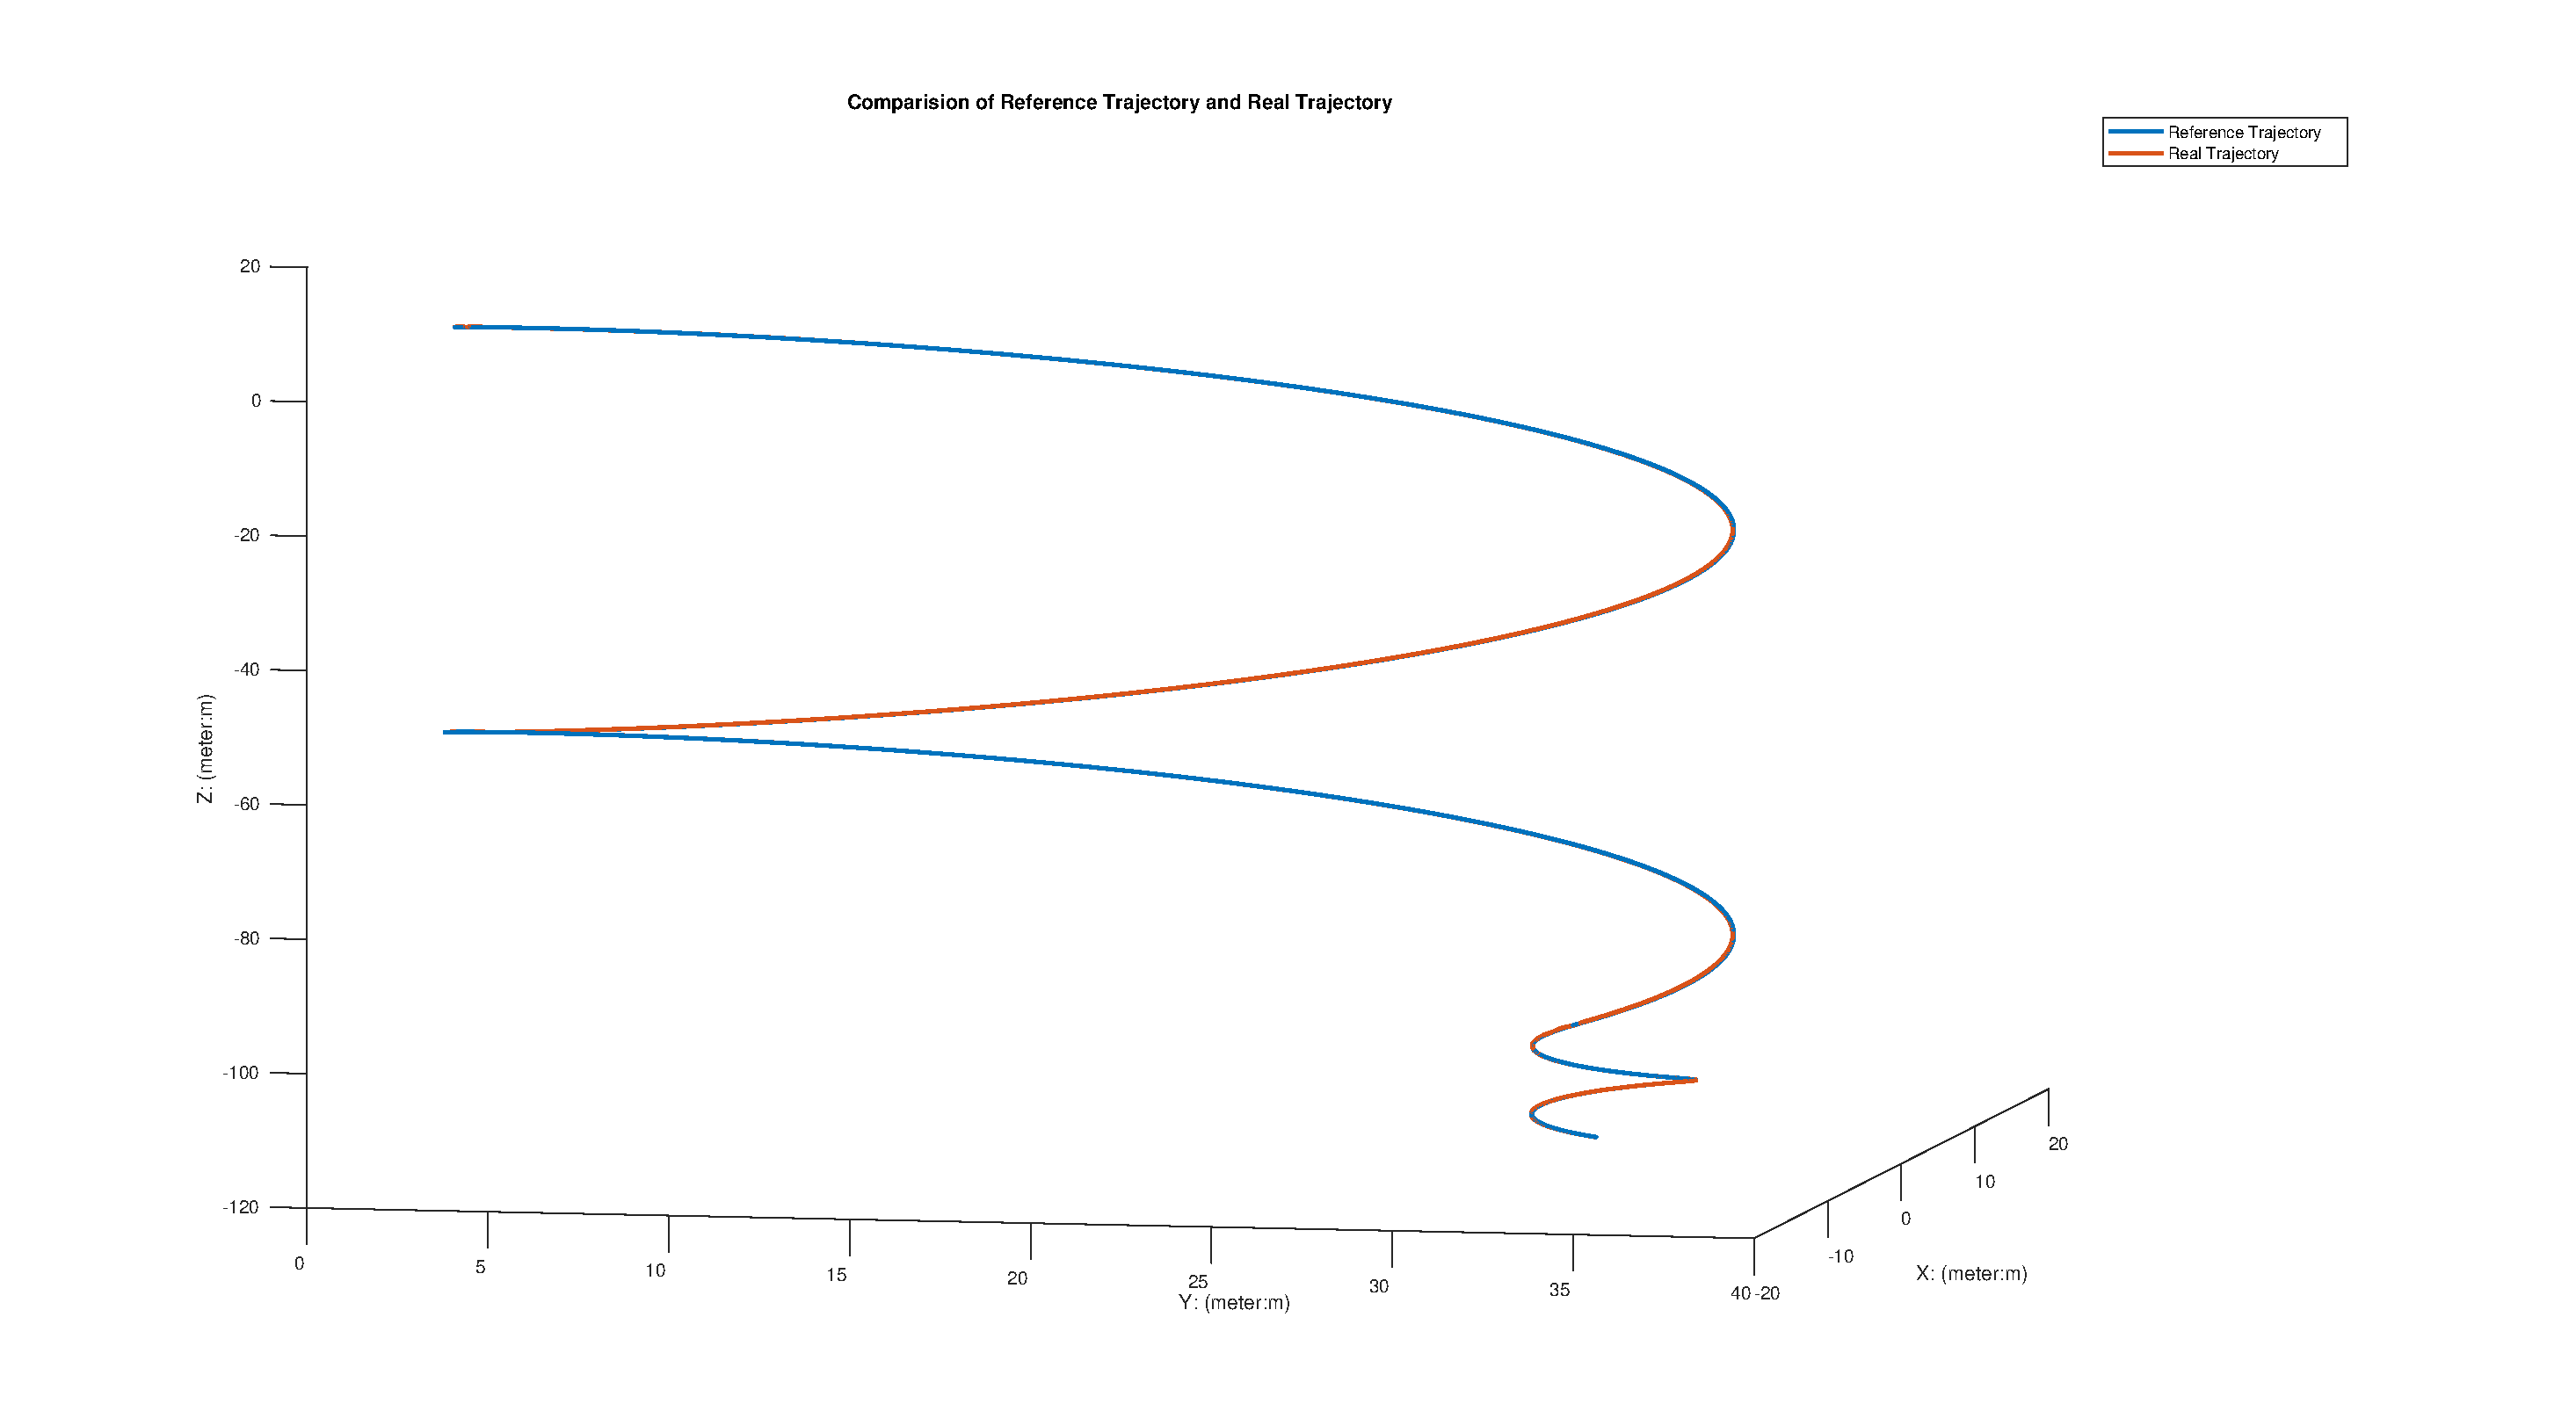
\includegraphics[width=\textwidth]{TrackUnsatTT.eps}
\caption{Comparison of desired trajectory and real trajectory (6 thrusters, no actuator saturation, train and test)}	
\label{FIG:TrackUnsatTT}
\end{figure}
\begin{figure}[h]
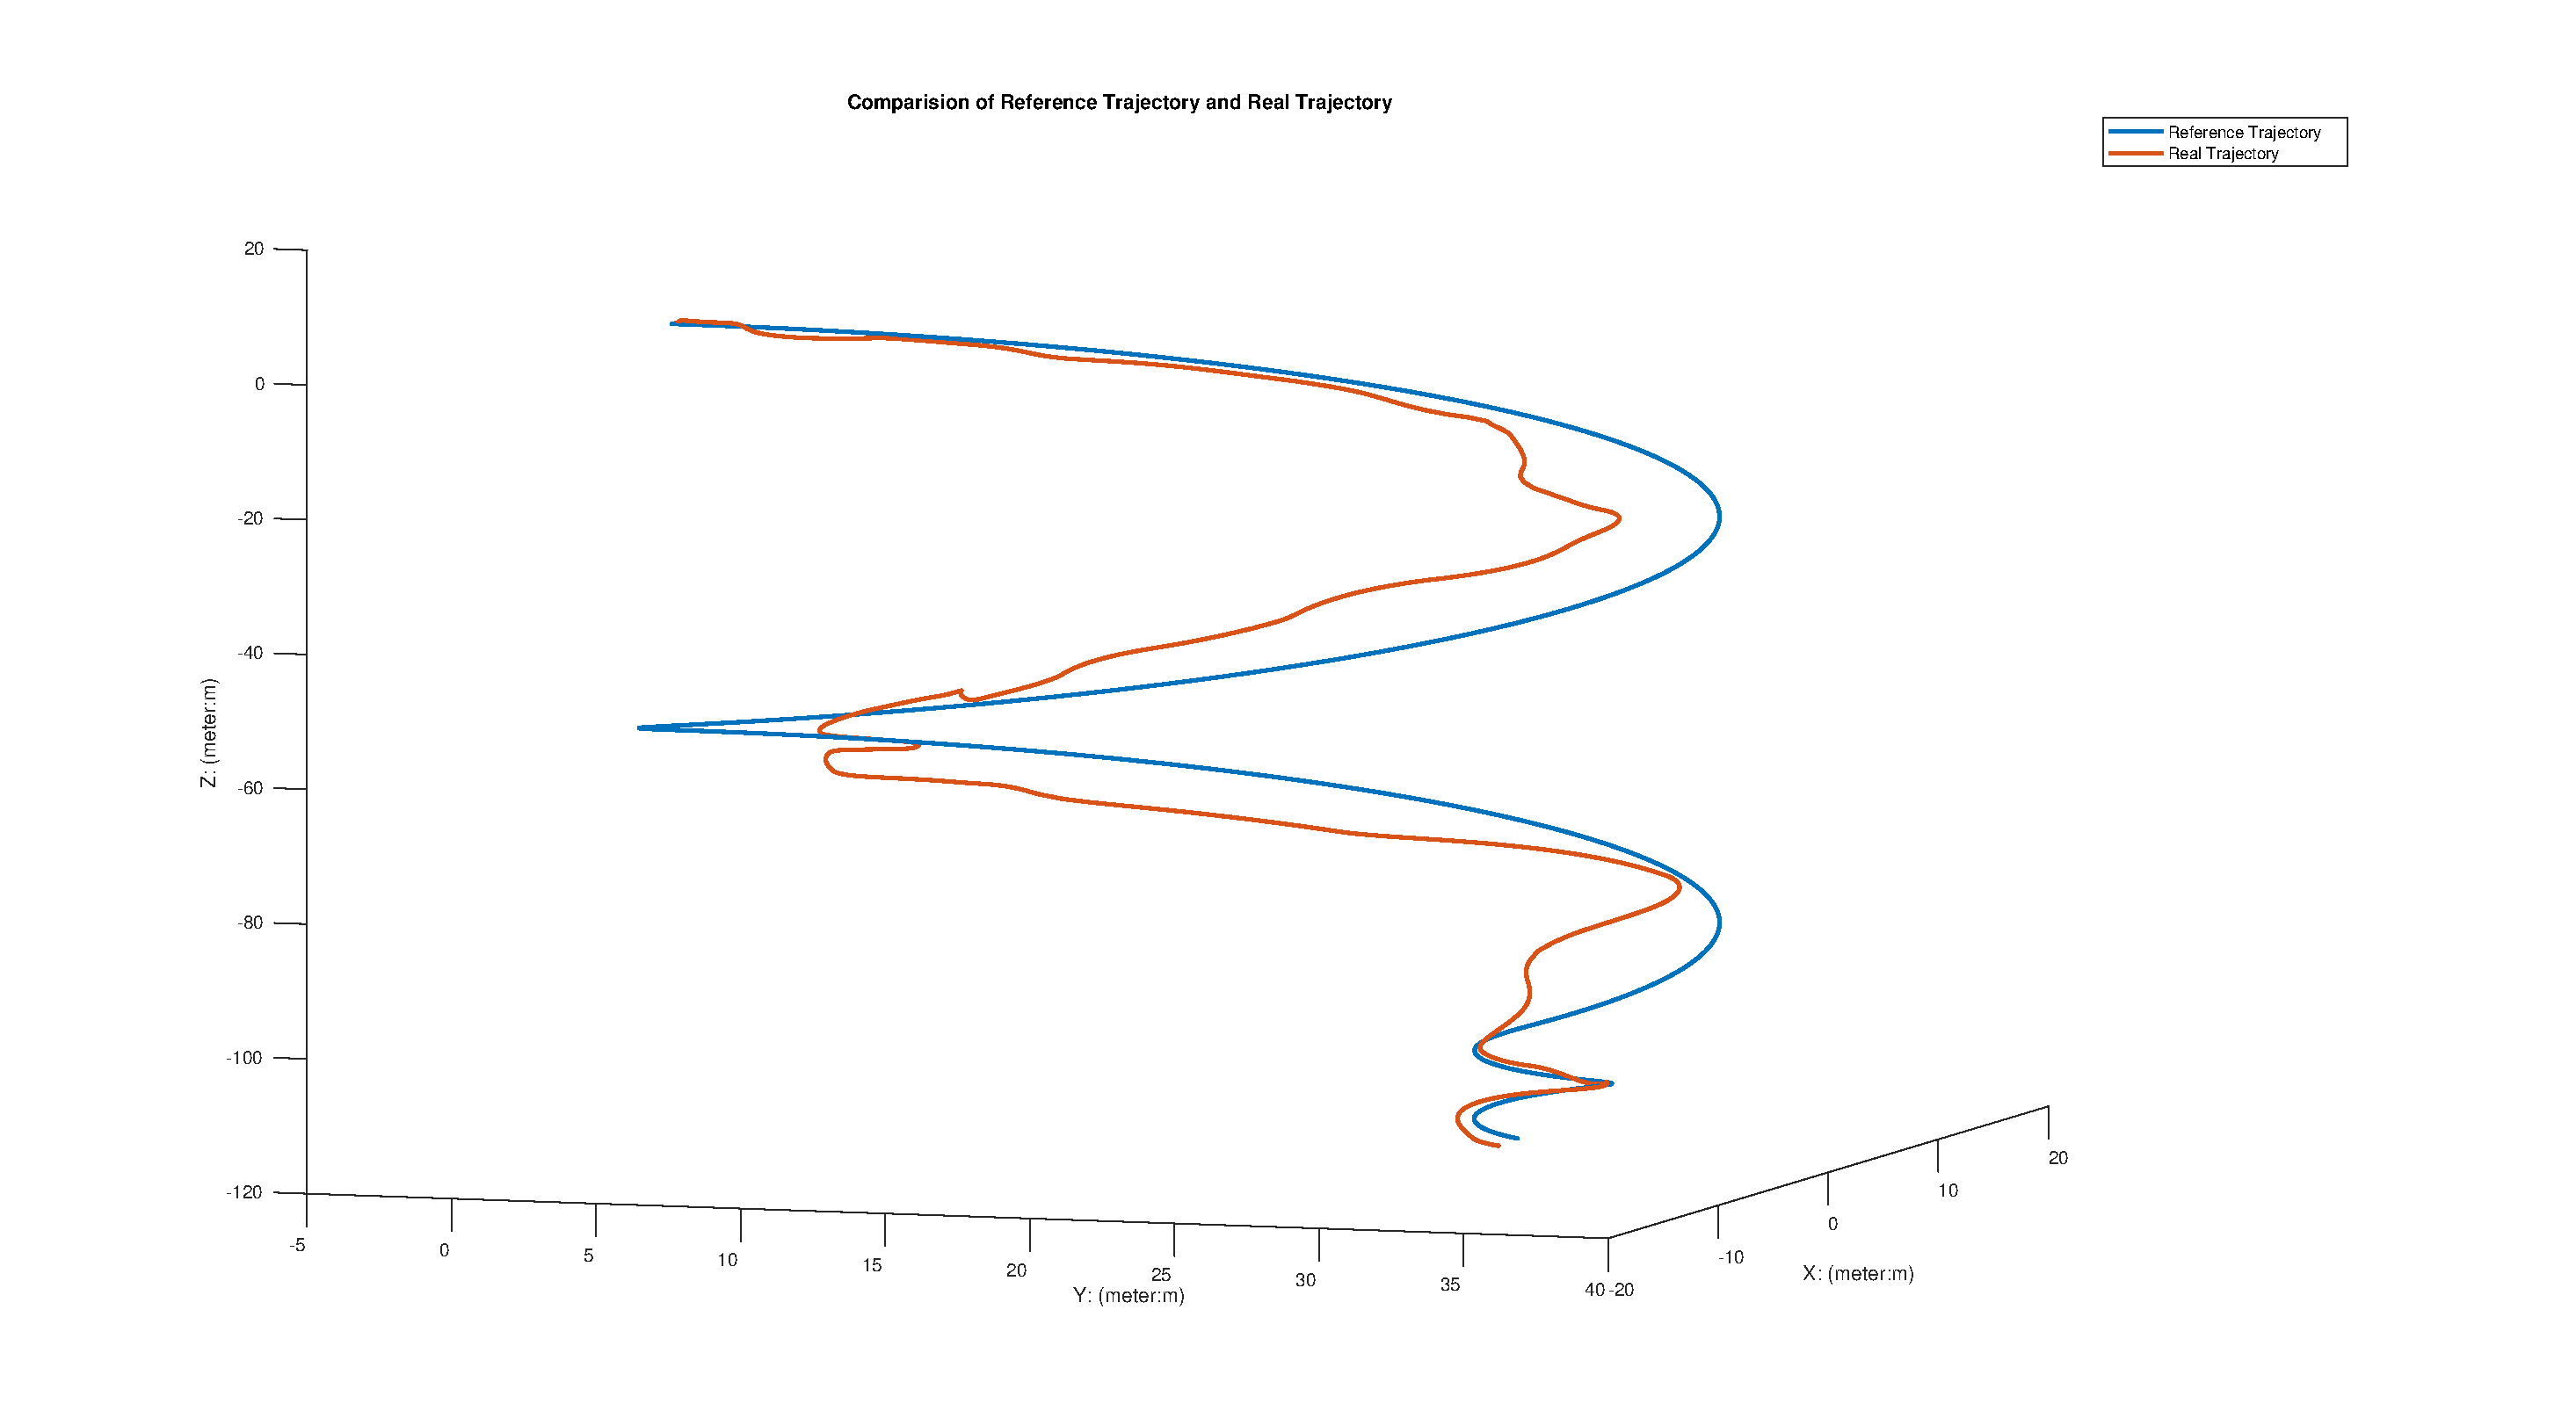
\includegraphics[width=\textwidth]{TrackSatTT.eps}
\caption{Comparison of desired trajectory and real trajectory (6 thrusters, with actuator saturation, train and test)}	
\label{FIG:TrackSatTT}
\end{figure}
%%%%%%%%%%%%%%%%%%%%%%%%%%%%%%%%%%%%%%%%%%%%%%%%%%%%%%%%%%%%%%%%%%%%%%%%%%%%%%%%%%
\section{Simulation for 4 Fins and 2 Thrusters} 
Compared with pure thrusters configuration, the placement of fins deserves further study since they are trajectory dependent. Not only the geometric variables concerning fins but also the trim specifications will contribute to the generated generalized force. Assume that the robot now has 4 fins and 2 thrusters to control its motion. In this case, we also set $\epsilon=0.001\times\dfrac{1}{7}\sum_{j=1}^{7}||\emph{\textbf{C}}_{E,j}^{1}||$.
%%%%%%%%%%%%%%%%%%%%%%%%%%%%%%%%%%%%%%%%%%%%%%%%%%%%%%%%%%%%%%%%%%%%%%%%%%%%%

As depicted in Figures~\ref{FIG:GeoVisualFinThruster21} and~\ref{FIG:GeoVisualFinThruster22}, the fins allocation in this case is quasi-symmetrical, two fins are located on the right front hull and other two are located on the left tail part of the hull. One thruster points to the right front side while other points to the left front side.  
\begin{figure}
\center
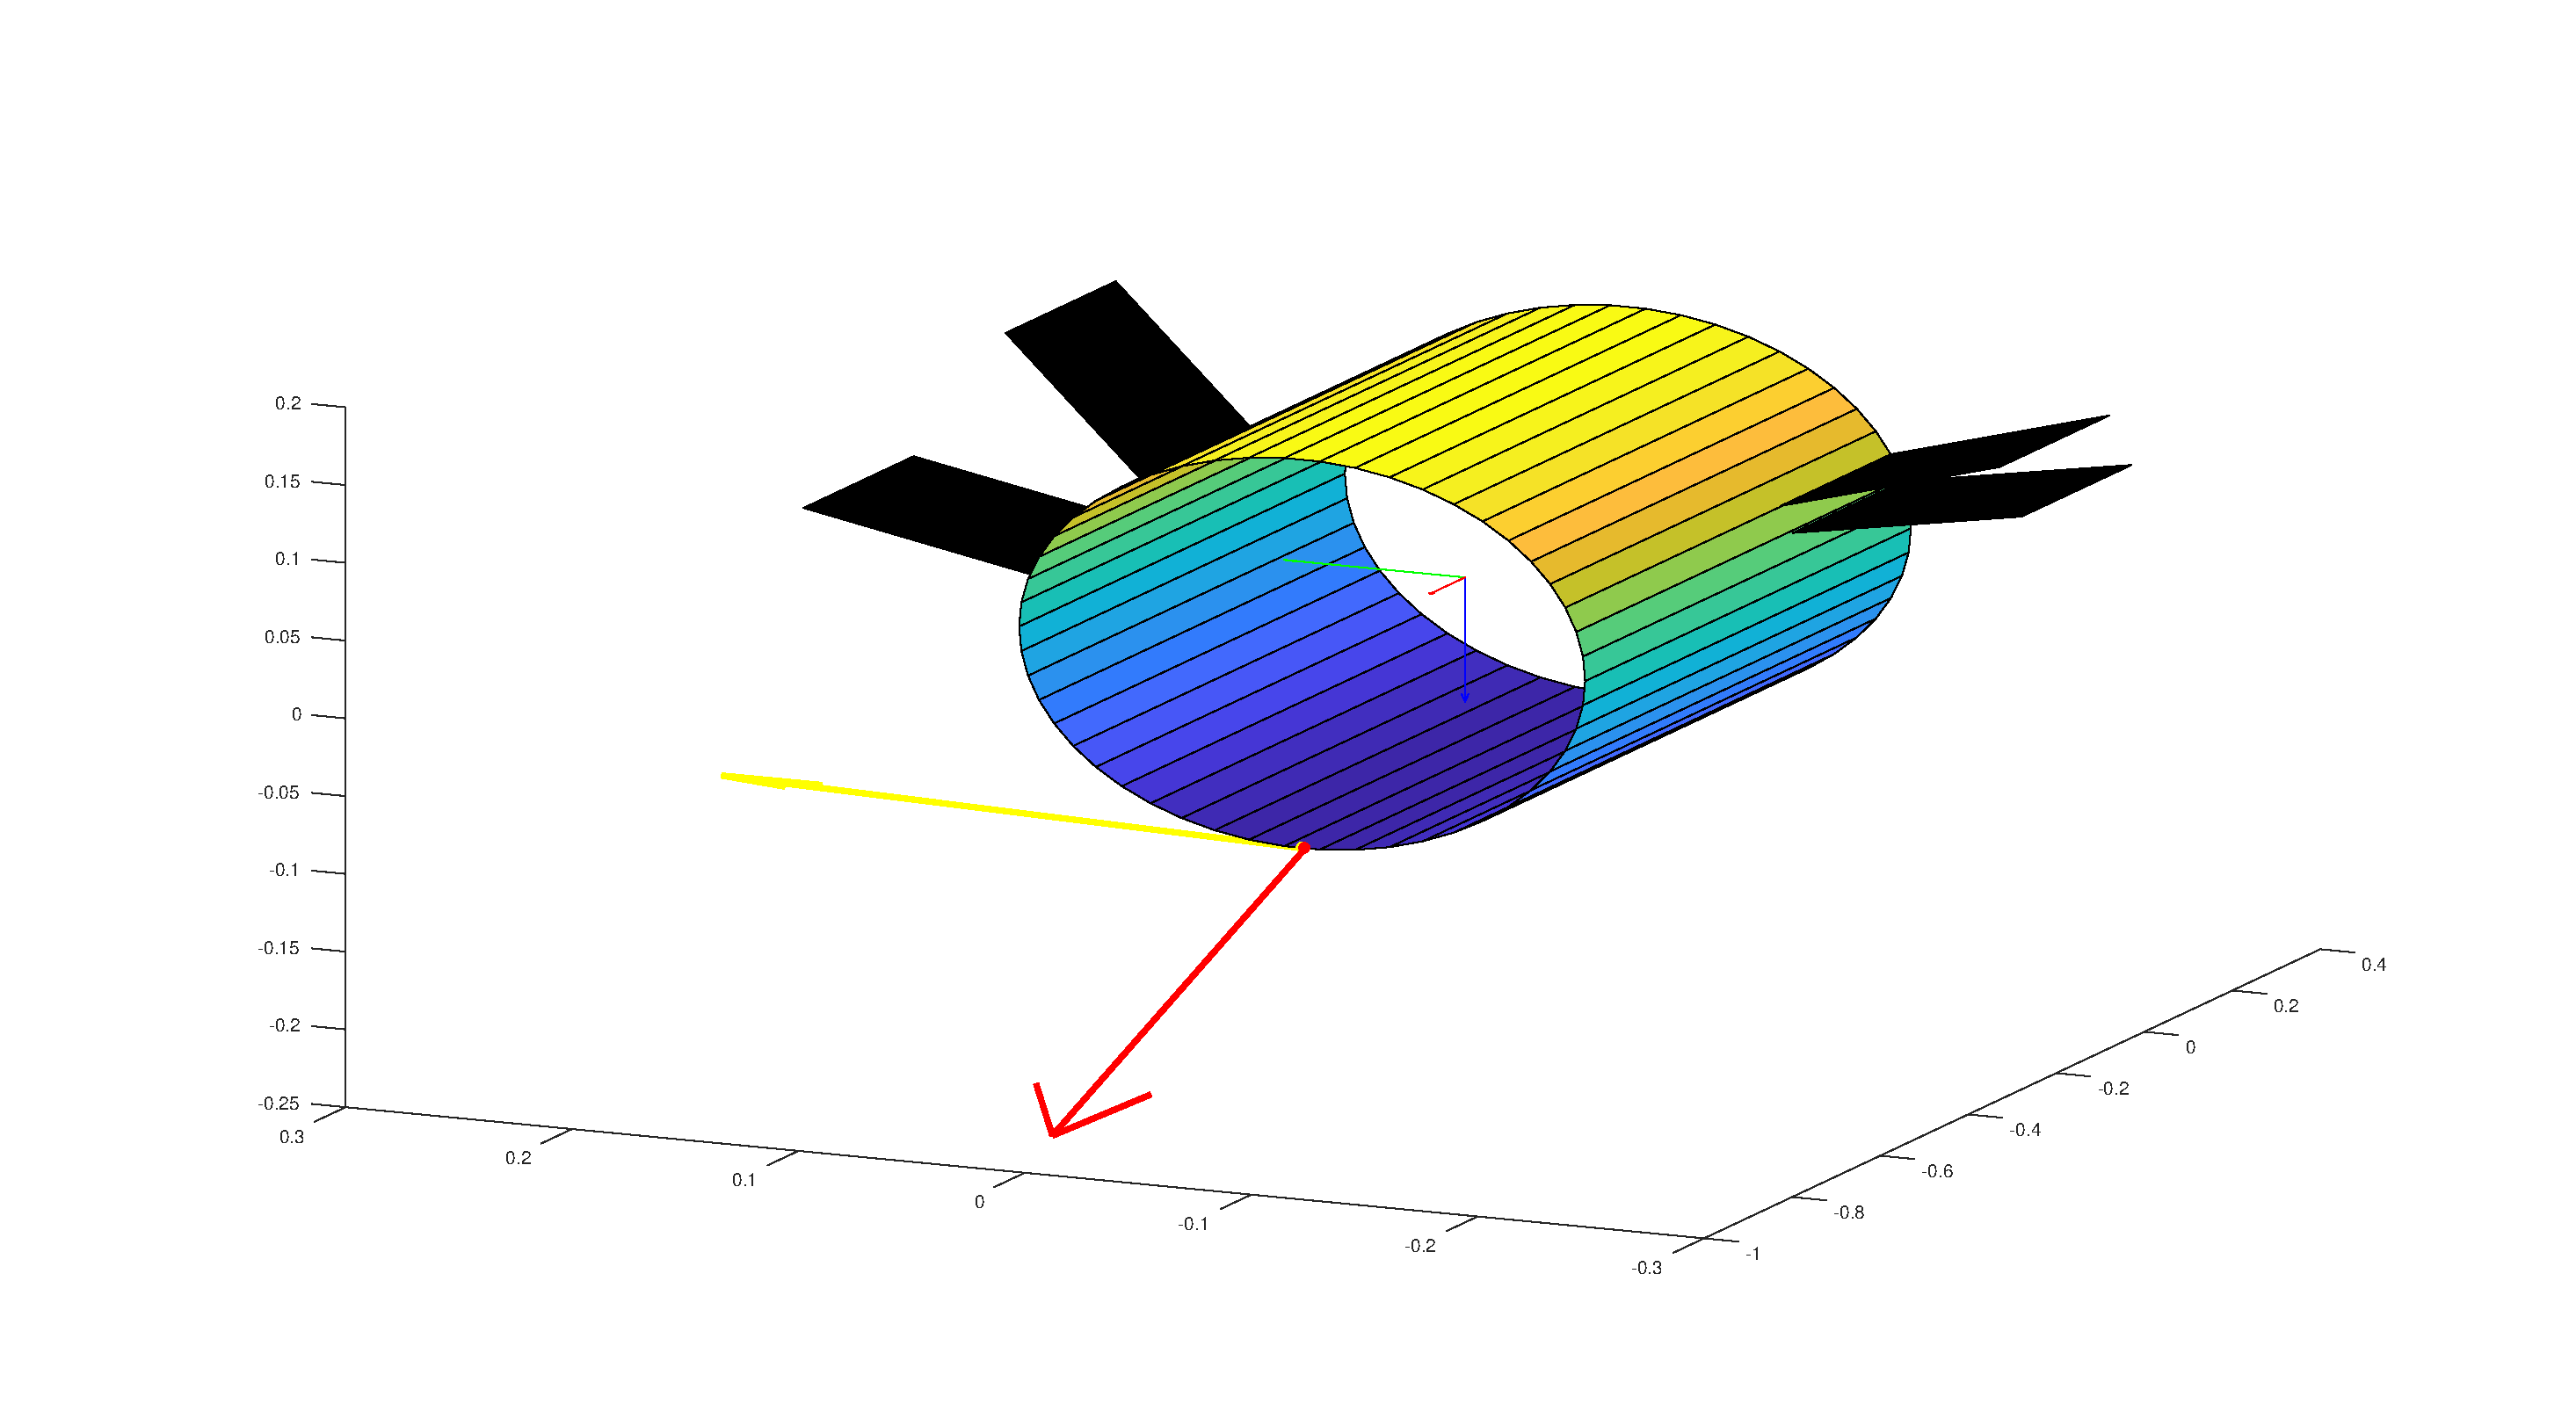
\includegraphics[width=0.9\textwidth]{GeoVisualFinThruster21.eps}
\caption{Visualization of optimization result (4 fins and 2 thrusters) perspective 1}	
\label{FIG:GeoVisualFinThruster21}
\end{figure}
\begin{figure}
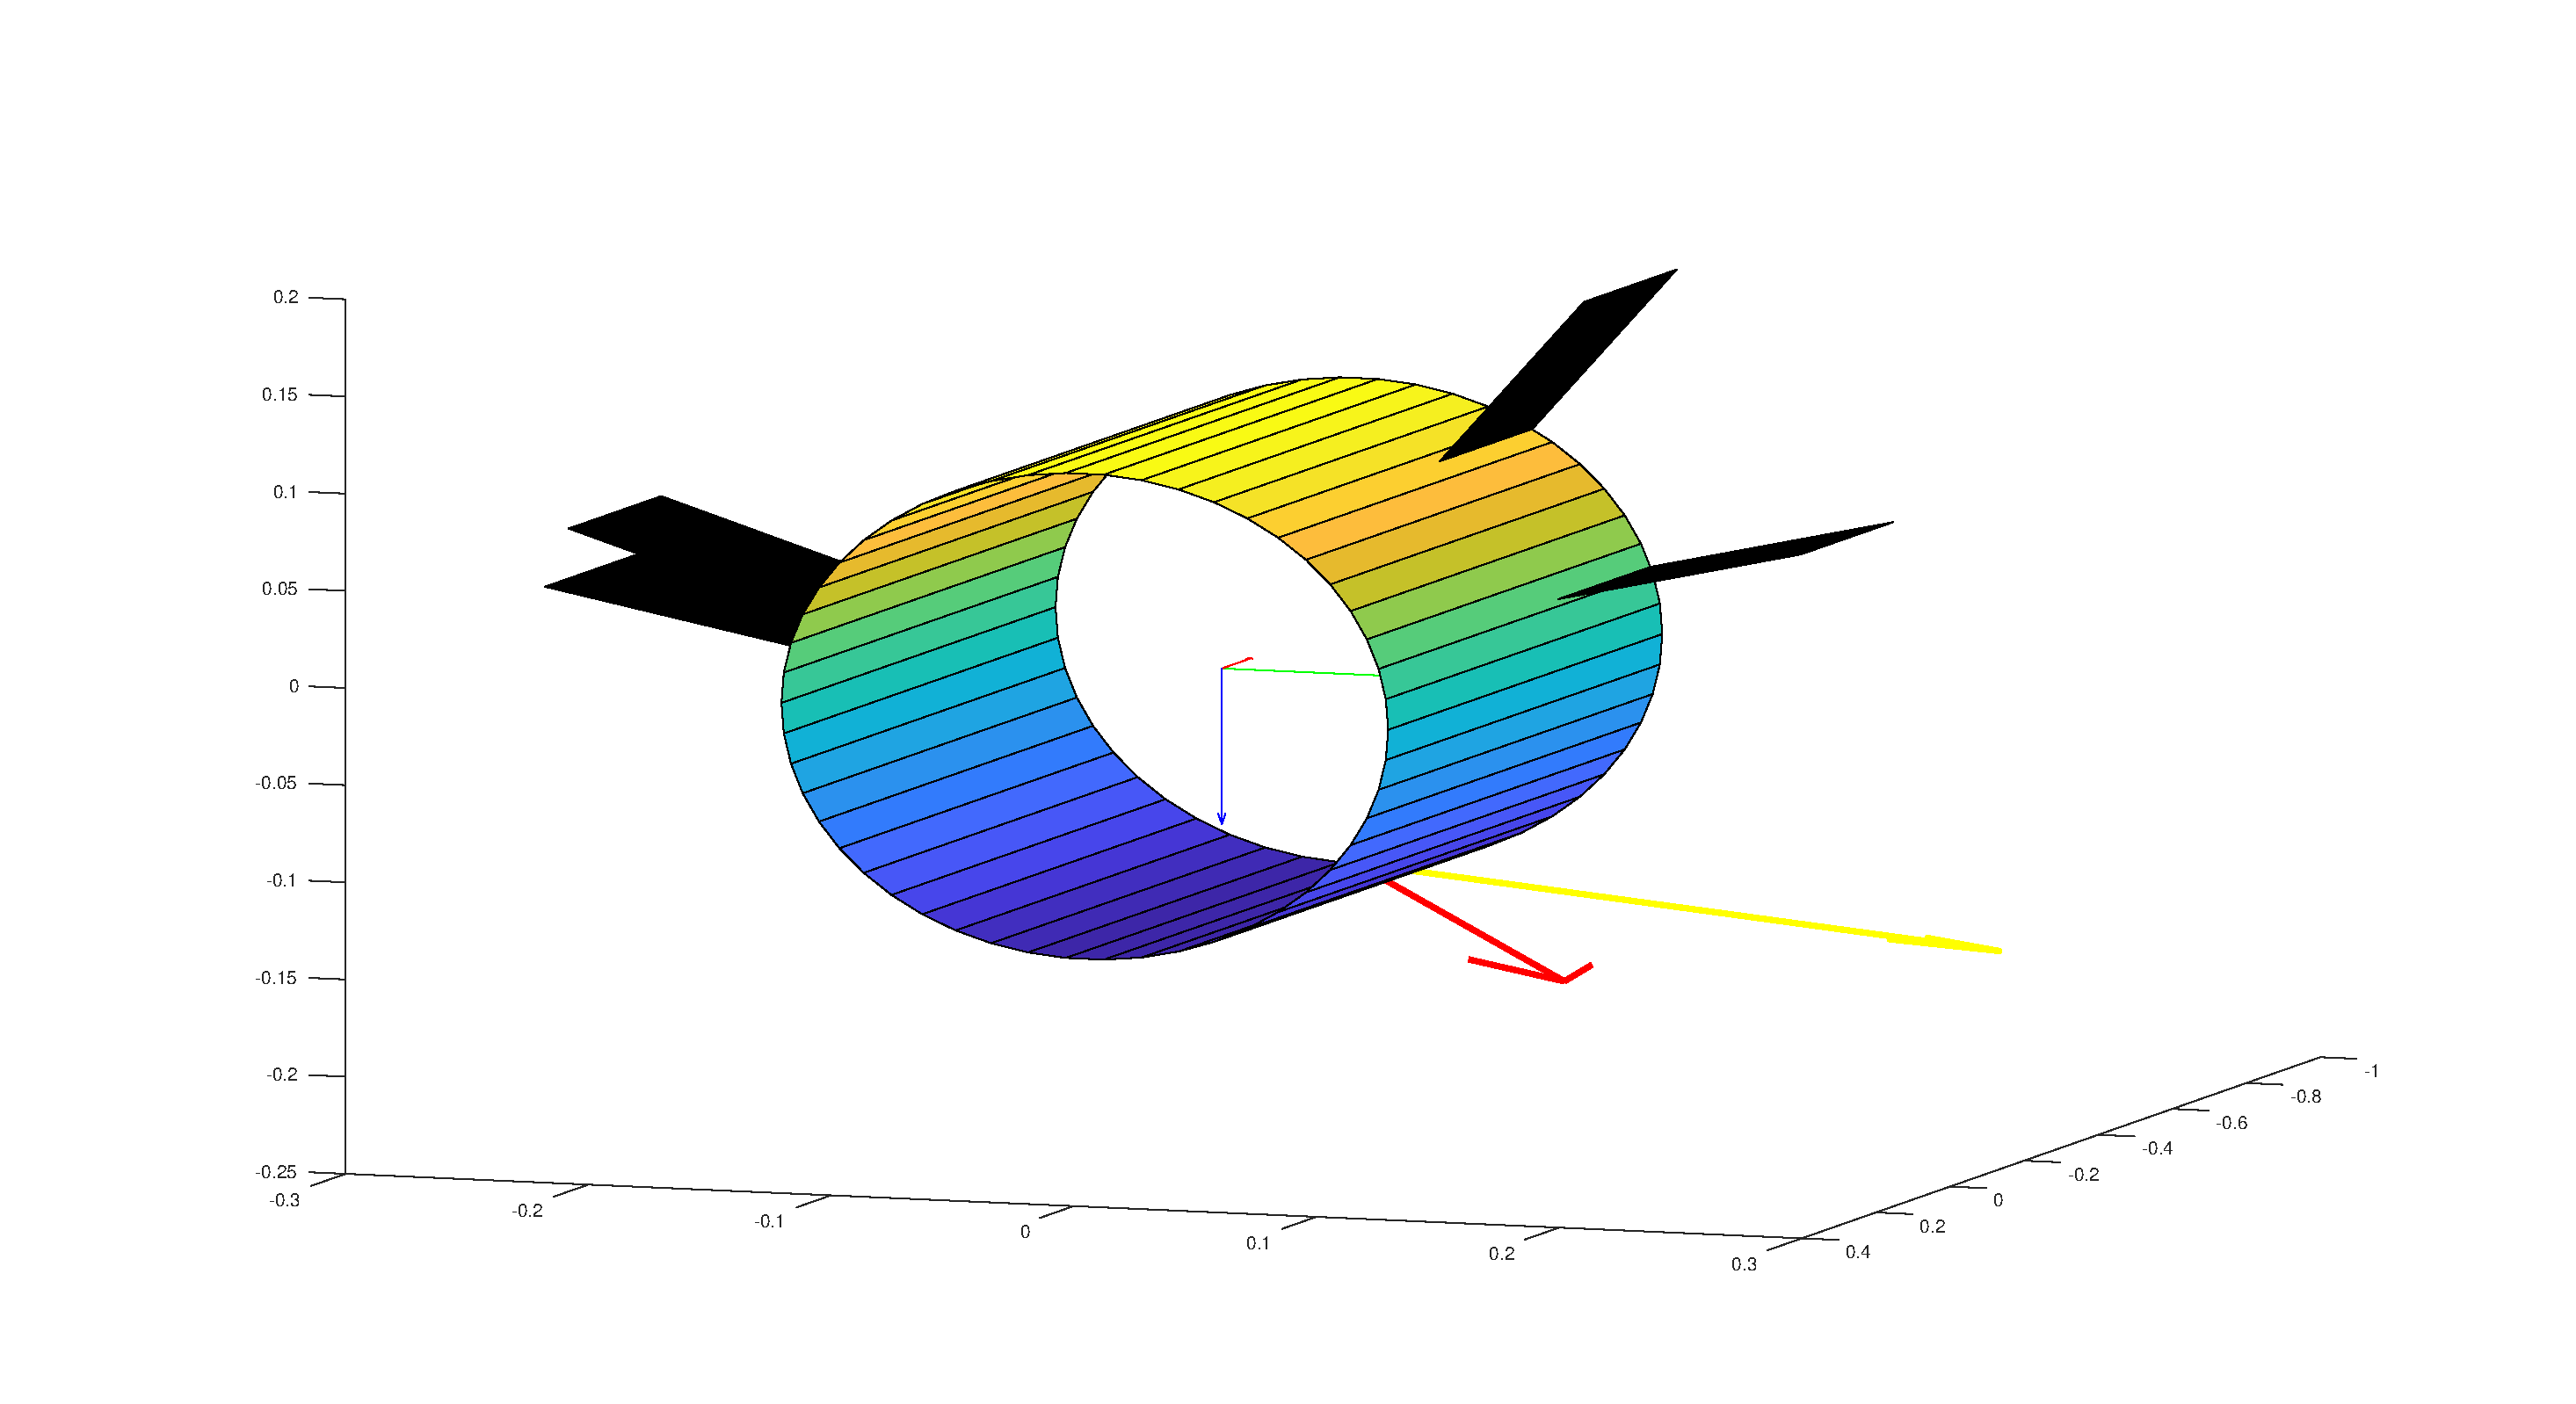
\includegraphics[width=\textwidth]{GeoVisualFinThruster22.eps}
\caption{Visualization of optimization result (4 fins and 2 thrusters) perspective 2}	
\label{FIG:GeoVisualFinThruster22}
\end{figure}
%%%%%%%%%%%%%%%%%%%%%%%%%%%%%%%%%%%%%%%%%%%%%%%%%%%%%%%%%%%%%%%%%%%%%%%%%%%%%%%%
From Figures~\ref{FIG:ConFin12},~\ref{FIG:ConFin22},~\ref{FIG:ConFin32} and~\ref{FIG:ConFin42}, we can see that the positions $x_{F,1}$, $x_{F,2}$, $x_{F,3}$ and $x_{F,4}$ stay constant after about 38 iterations, while the orientations keep on changing. It can be seen from Figures \ref{FIG:ConThruster12} and \ref{FIG:ConThruster22} that the positions and orientations of thruster 1 and thruster 2 converge after about 50 iterations. 
\begin{figure}
\includegraphics[width=0.5\textwidth]{ConFin1Pos2.eps}
\includegraphics[width=0.5\textwidth]{ConFin1Orient2.eps}
\caption{Convergence of position and orientation of fin 1 (4 fins and 2 thrusters)}	
\label{FIG:ConFin12}
\end{figure}
\begin{figure}
\includegraphics[width=0.5\textwidth]{ConFin2Pos2.eps}
\includegraphics[width=0.5\textwidth]{ConFin2Orient2.eps}
\caption{Convergence of position and orientation of fin 2 (4 fins and 2 thrusters)}	
\label{FIG:ConFin22}
\end{figure}
\begin{figure}
\includegraphics[width=0.5\textwidth]{ConFin3Pos2.eps}
\includegraphics[width=0.5\textwidth]{ConFin3Orient2.eps}
\caption{Convergence of position and orientation of fin 3 (4 fins and 2 thrusters)}	
\label{FIG:ConFin32}
\end{figure}
\begin{figure}
\includegraphics[width=0.5\textwidth]{ConFin4Pos2.eps}
\includegraphics[width=0.5\textwidth]{ConFin4Orient2.eps}
\caption{Convergence of position and orientation of fin 4 (4 fins and 2 thrusters)}	
\label{FIG:ConFin42}
\end{figure}
\begin{figure}
\includegraphics[width=0.5\textwidth]{ConThruster1Pos2.eps}
\includegraphics[width=0.5\textwidth]{ConThruster1Dir2.eps}
\caption{Convergence of position and direction of thruster 1 (4 fins and 2 thrusters)}	
\label{FIG:ConThruster12}
\end{figure}
\begin{figure}
\includegraphics[width=0.5\textwidth]{ConThruster2Pos2.eps}
\includegraphics[width=0.5\textwidth]{ConThruster2Dir2.eps}
\caption{Convergence of position and direction of thruster 2}	
\label{FIG:ConThruster22}
\end{figure}
\begin{figure}
\centering
\includegraphics[width=0.75\textwidth]{ConNorm2.eps}
\caption{Convergence of error dynamics controllability matrix norm (4 fins and 2 thrusters)}	
\label{FIG:ConNorm2}
\end{figure}
\newpage
%%%%%%%%%%%%%%%%%%%%%%%%%%%%%%%%%%%%%%%%%%%%%%%%%%%%%%%%%%%%%%%%%%%%%%%%%%%%%%%%%
The value of the control input objective function $fval_{input}$ increases at first and then falls down sharply from the 5-th iteration to the 10-th iteration. Afterwards, it restarts to increase until the 30-th iteration and then falls down again. The position optimization objective function $fval_{pos}$ rises sharply in the beginning but decreases quickly to about 50. 
\begin{figure}
\center
\includegraphics[width=0.49\textwidth]{ConInput2.eps}
\includegraphics[width=0.49\textwidth]{ConPos2.eps}
\caption{Value of objective function (4 fins and 2 thrusters)}	
\label{FIG:ConPosInput2}
\end{figure}
\newpage
%%%%%%%%%%%%%%%%%%%%%%%%%%%%%%%%%%%%%%%%%%%%%%%%%%%%%%%%%%%%%%%%%%%%%%%%%%
We use the state and input cost matrices in Table~\ref{table:QParameters} and Table~\ref{table:RParameters for 4 fins and 2 thrusters} to design the switched LQR controller. Note that in this case smaller input weighting matrices are chosen meaning larger control inputs are needed to track the desired trajectory.  
\begin{table}
\centering
\small
\caption{Input cost matrices for 4 fins and 2 thrusters}
\begin{tabular}{| c | c | c | c | p{0.5cm} |}
\hline
Index&$\mathcal{R}_{E}$ \\ \hline
1&diag([0.0001,0.0001,0.0001,0.0001,0.0001,0.0001])\\ \hline
2&diag[0.00001,0.00001,0.00001,0.00001,0.00001,0.00001] \\ \hline
3&diag([0.00001,0.00001,0.00001,0.00001,0.00001,0.00001])\\ \hline
4&diag([0.00001,0.00001,0.00001,0.00001,0.00001,0.00001]) \\ \hline
5&diag([0.00001,0.00001,0.00001,0.00001,0.00001,0.00001])\\ \hline
6&diag([0.00001,0.00001,0.00001,0.00001,0.00001,0.00001])\\ \hline
7&diag([0.001,0.001,0.001,0.001,0.001,0.001]) \\ \hline
\end{tabular}
\label{table:RParameters for 4 fins and 2 thrusters}
\end{table}
%%%%%%%%%%%%%%%%%%%%%%%%%%%%%%%%%%%%%%%%%%%%%%%%%%%%%%%%%%%%%%%%%%%%%%%%%%%%%%
As depicted in Figure~\ref{FIG:TrackUnsat2}, the robot with current optimized realize perfect tracking without actuator capability constraints with same weighting matrices. When the thrust is restricted to $[-35,40]$ N and the deflection is constrained in $[-\pi,\pi]$ rad, as depicted in Figure~\ref{FIG:TrackSat2}, the real trajectory preserves the fundamental characteristic of the reference trajectory roughly, although the deviation is still large.
\begin{figure}
\includegraphics[width=0.75\textwidth]{TrackUnsat2.eps}
\caption{Comparison of desired trajectory and real trajectory (4 fins and 2 thrusters, no actuator saturation)}	
\label{FIG:TrackUnsat2}
\end{figure}
\begin{figure}
\includegraphics[width=0.75\textwidth]{TrackSat2.eps}
\caption{Comparison of desired trajectory and real trajectory (4 fins and 2 thrusters, with actuator saturation)}	
\label{FIG:TrackSat2}
\end{figure}

%%%%%%%%%%%%%%%%%%%%%%%%%%%%%%%%%%%%%%%%%%%%%%%%%%%%%%%%%%%%%%%%%%%%%%%%%%%%%%%%%%
\section{Summary}
It can be concluded from these simulation results that our optimization algorithm is able to find locally optimal geometric configurations depending on the randomly generated initial values. By means of the multi-stage iterative optimization in the algorithm, the control input objective function and the position objective function can also be minimized to a small value but not zero. Normally, the geometric configuration at the breaking iteration corresponds to the least average condition number and thus is chosen as optimal value. 

Without consideration of actuator's capability, a nearly perfect tracking is realizable for different actuator configurations by tuning input and state weighting matrices appropriately. However, in realistic situations, the robot with only thrusters tracks the desired trim trajectories unstably while the robot using fins with thrusters as actuators perform worse with considerably large tracking error. For LQR controller, the limitations of actuators are not taken into consideration which influence the tracking performance of the underwater robots heavily. Thus, it is recommendable to choose switched Model Predictive Controller (MPC) to control the robot. The main differences between MPC and LQR are that LQR optimizes in a fixed horizon whereas MPC in a receding horizon and that the optimal control input is calculated at each step where as LQR uses the single optimal value for the whole horizon. Hence, MPC allows real-time optimization against hard constraints~\cite{Wang2009} which can enhance the tracking performance of the underwater robots.

 








%_____Zusammenfassung, Ausblick_________________________________
\chapter{Conclusion and Future Work}
\section{Conclusion}
%Standard underwater robots are normally equipped with fins and actuators in pairs symmetrically. In this work, we propose a design process to build nonstandard underwater robots by formulating it as multi-stage iterative optimization problems optimized for the kinematic, dynamic specifications and other specific design goals.

In this thesis, we introduce an approach for designing underwater robots computationally by formulating the design procedure as multi-stage iterative optimizations according to design specifications. The distinguishing novelty of our work is that we obtain design requirements from the desired trajectories. In addition, Frenet-Serret frame is selected such that the surge velocity is tangent to the trim trajectory curve and direction of other velocities are consequently specified. 

%More precisely, the following 11 states are constant:
%\begin{itemize}
%\item The surge ($u$), sway ($v$) and heave ($w$) velocities;
%\item The roll ($p$), pitch ($q$) and yaw ($r$) velocities;
%\item The roll angle ($\phi$) and pitch angle ($\theta$).
%\end{itemize}
We use trim trajectories to represent the robot's motion paths since the robot moves stably, i.e., all 12 states except for the yaw angle $\psi$ are constant. 
%The velocities influence the added mass inertia matrix $\emph{\textbf{M}}_{A}$, the Coriolis matrices $\emph{\textbf{C}}_{RB}$ and $\emph{\textbf{C}}_{A}$ and the damping matrix $\emph{\textbf{D}}$. The roll $\phi$ and pitch angle $\theta$ influence the restoring term $\vec{g}(\vec{\eta})$. For a trim trajectory segment, the aforementioned 
%11 states do not change ($\vec{\upsilon}$ and $\Pi_{i}\vec{\lambda}$ are constants) and thus the underwater robot dynamics is constant for a given robot geometric structure. This explains the meaning of the stable motion along trim trajectories.
Another decisive reason for selecting trim trajectories is that we can build the error dynamics using nonlinear tranformations~\ref{EQ:NLT1}, \ref{EQ:NLT2}, \ref{EQ:NLT3} and \ref{EQ:NLT4} whose linearization is unique. The nonlinear underwater dynamics can be transformed into MIMO linear system parametrized by trim trajectory specifications. In this way, a number of analysis and design methods for linear systems can be implemented. More importantly, trajectories' information is brought into the robot dynamics. Therefore, it is reasonable to state that the underwater robot geometry is defined by the trim trajectories. 

%If we are given a set of trim trajectories $\mathcal{T}_{1}, \cdots, \mathcal{T}_{m}$, we have the information about $(x_{\mathcal{T}_{1}}, y_{\mathcal{T}_{1}}, z_{\mathcal{T}_{1}})^{T}, \cdots, (x_{\mathcal{T}_{m}}, y_{\mathcal{T}_{m}}, z_{\mathcal{T}_{m}})^{T}$, where $(x_{\mathcal{T}_{j}}, y_{\mathcal{T}_{j}}, z_{\mathcal{T}_{j}})^{T}, j=1, \cdots, m$ denotes the desired trim positions in the inertial world frame $\lbrace i \rbrace$.

%By using the Frenet-Serret frame, we have the information about $(\phi_{\mathcal{T}_{1}}, \theta_{\mathcal{T}_{1}}, \psi_{\mathcal{T}_{1}})^{T}, \cdots,\\ (\phi_{\mathcal{T}_{m}}, \theta_{\mathcal{T}_{m}}, \psi_{\mathcal{T}_{m}})^{T}$, where $(\phi_{\mathcal{T}_{j}}, \theta_{\mathcal{T}_{j}}, \psi_{\mathcal{T}_{j}})^{T}, j=1, \cdots, m$ denotes the desired trim Euler angles in the inertial world frame $\lbrace i \rbrace$. From the Euler angles we can calculate the corresponding linear velocity transformation matrix $\emph{\textbf{R}}$ and angular velocity transformation matrix $\emph{\textbf{Q}}$. Combing all of them, we obtain the trim linear velocities $\vec{v}_{\mathcal{T}_{1}}, \cdots, \vec{v}_{\mathcal{T}_{m}}$ and trim angular velocities $\vec{\omega}_{\mathcal{T}_{1}}, \cdots, \vec{\omega}_{\mathcal{T}_{m}}$ 
%which specify the desired dynamic behaviour when the robot tracks the specified trim trajectories perfectly. Starting from the trim position specifications, we are able to derive the full specifications of robot kinematics and dynamics. 

Besides, the conventional underwater robot design requirements (buoyancy neutral, surge velocity maximization, energy storage maximization, cost minimization and compact structure) must also be taken into consideration. 

Because we deign the underwater robot in an iterative way, the robot geometry will be updated continuously. Therefore, an customizable robot dynamics determined by these geometric parameters is aimed for.  
Based on this requirement, we propose a modular modeling method. All consisting modules of the robot will be represented by simple geometric shapes determined with several geometric variables so that we can construct and reconfigure the robot easily. These geometric variables will be identified as decision variables and consequently the robot dynamics can be parametrized by them.
 
%The robot decision variables can be divided into four groups:
%\begin{itemize}
%\item The hull decision variables group: $\mathfrak{d}_{H}$;
%\item The spin direction of the thrusters $b_{1}, \cdots, b_{n_{t}}$;
%\item The positions decision variables group: thrusters positions $r_{T,1}, \cdots, r_{T,n_{t}}$ and fins positions $x_{F,1}, \cdots, x_{F,n_{f}}$;
%\item The orientations of thrusters and fins: thruster orientations $\vec{d}_{T,1}, \cdots, \vec{d}_{T,n_{t}}$ and fins orientations $\gamma_{F,1}, \cdots, \gamma_{F,n_{f}}$.
%\end{itemize}
%To obtain feasible solution of an optimal robot geometry, it is necessary to %decouple these decision variables into several optimization stages.

%To sum up, our goal is to design the robot, i.e., determining the values of these four groups of decision variables satisfying the previous discussed two groups of specifications.

By studying the relationship between the robot dynamics and the geometric decision variables we find that there are strong couplings among these geometric parameters. 

The main approach to obtaining a feasible solution of an optimal robot geometry is to decouple these decision variables. Since the hull parameters couple with all other decision variables, the first step is to decouple the hull decision variables. This motivates us to separate the hull optimization and the actuator placement optimization. The hull parameters will be determined in the first phase and set as constant for further optimizations steps. The spin directions are discrete decision variables, thus they are determined in the beginning of the actuator optimization according to the average error dynamics condition number and separated from positions and orientations parameters. The positions and orientations of fins and thrusters as well as the control inputs (thrust forces and deflection angles) are decoupled in an iterative way. We optimize the control inputs at the first stage and keep the positions and orientations as unchanged. Similarly, the optimization of positions are based on the assumption that the control inputs and the orientations are constant. At the third optimization stage of orientation, the control inputs and positions are fixed. By means of these iterative multi-stage optimization approaches the decision variables are totally decoupled. 

As we obtain a set of MIMO linearized error dynamic systems from the trim trajectories, we are able to formulate the total system as a linear switched system. Consequently, we utilize the switched LQR controller for our system. All input and state weighting matrices influence the stability of the system together.  
Thus, a method to select their values is proposed in this work based on the stability analysis by common Lyapunov function. 

Finally, it can be concluded from the simulation results in Chapter 6 that the users are able to utilize our designing procedure to design an underwater robot prototype with locally optimized geometry adapting to the training trim trajectories. With the optimized actuator configuration the underwater robot system is controllable and can track the desired paths stably using the switched LQR controller. However, if the actuator capabilities are taken into account, the switched LQR controller works unsatisfactorily and the robot could not track the desired trajectories accurately.
 
\section{Limitations and Future Work}
This is a pioneer research work, thus we make a list of assumptions and there exists limitations which can be rectified and optimized for the future works.
\subsection{Prototype Modeling}
The accuracy of customizable modelling of underwater robots plays an essential role for the result of the optimization algorithms. However, due to the nature of nonlinearity in the robot dynamics, there exists couplings among the geometric decision variables. In our work, we adopt a series of assumptions to obtain a feasible solution.

The hydrodynamic effects are the main source for nonlinearities. We simplify the  calculation by assuming only the robot hull contributes to the hydrodynamic effects. However, it is not true in reality.

The robot hull is also influenced by the lift force but we neglect it.  Fins are modeled as rectangular plate whose added mass should also be calculated and transformed into the robot dynamics. Also, fins affect the hydrodynamic damping coefficients. Furthermore, as a significant component of the robot prototype, in this thesis, we pay attention on thruster's functionality to generate forces and moments but ignore their contributions to hydrodynamic effects as a geometric shape. According to~\cite{Sia1999}, the thruster housings can also be modeled as hollow cylinder similar to hull enclosure and the water bodies within the thruster can be modeled as solid cylinders like the batteries. Both of them should be considered for added mass coefficients and damping coefficient estimation in future work.

By calculation of the robot's total moment of inertia, we merely take the hull components (hull enclosure, batteries and electronic devices) into consideration. For a more accurate modeling , the actuator moment of inertia should also be considered. Note that the moment of inertia for actuators is given with respect to their own center of mass. It should be transformed into the robot body frame $\lbrace b \rbrace$ using equations~\ref{EQ:MomentTransfer1}, \ref{EQ:MomentTransfer2}, \ref{EQ:MomentTransfer3} whose values are determined by their position in the body frame. Thus, in the main 
optimization, not only the center of gravity $\vec{r}_{G}$ but also the robot moment of inertia $\emph{\textbf{I}}_{g}$ should be updated after the geometric decision variables $\vec{r}_{T}$, $x_{F}$ and $\gamma_{F}$ are optimized. Both $\vec{r}_{G}$ and $\emph{\textbf{I}}_{g}$ affect the rigid body inertia matrix $\emph{\textbf{M}}_{RB}$ (see~\ref{EQ:MRBCO}). 

The hydrodynamic modeling for fins in our work is only viable for very small angle of attack $\alpha$. The lift and drag coefficients $C_{L}$ and $C_{D}$ are assumed to be constant in this case. However, the angle of attack $\alpha$ affects them heavily. High order polynomial might be used to approximate the relationship between the attack angle $\alpha$ and the hydrodynamic coefficients $C_{L}$ and $C_{D}$. In Appendix~\ref{Appendix:AccurateHydrodynamicModeling}, an accurate hydrodynamic modeling is discussed. Besides, in our actuator optimization algorithm, the drag of fins is not treated as control input like the lift but as disturbance. In order to enhance the optimization quality, a more suitable fin modeling is desired.

Recall the thruster modeling in the Section~\ref{Subsection:ModelingofThrusters}, the moments generated by thrusters is composed of two parts: the rotation moment vector $\vec{m}_{T,r}=b_{T}\lambda_{T} u_{T}\vec{d}_{T}$ and the thrust moment $\vec{m}_{T,t}=\vec{r}_{T}\times u_{T}\vec{d}_{T}$. Strictly speaking, both of them are modeled inaccurately. For the rotation moment, we ignore the dynamics of the propeller and assume the rotation moment is proportional to the thrust. Furthermore, the thrust moment $\vec{m}_{T,t}$ should be calculated with respect to the robot center of gravity $CG$ instead of the body frame origin $CO$. Therefore, the thruster moment should be calculated in an accurate way as:
\begin{align}
\vec{m}_{T,t}=(\vec{r}_{T}-\vec{r}_{G})\times u_{T}\vec{d}_{T},
\end{align}
where $\vec{r}_{G}$ denotes the robot center of mass and $\vec{r}_{T}$ is the position the thruster in the body frame $\lbrace b \rbrace$. However, $r_{G}$ is updated at each optimization loop and computed from $\vec{r_{T}}$, $x_{F}$ and $\gamma_{F}$. Consequently, it brings coupling between $\mathfrak{d}_{P}$ and $\mathfrak{d}_{F}$ which is not expected. Therefore, we assume the center of gravity $CG$ is located in the body frame origin $CO$ for calculating the thrust moment. Nevertheless, for the future work these two simplified modelings can be made accurately. 

\subsection{Optimization Algorithms}
To make the optimization problems solvable, we perform a number of assumptions to decouple the geometric decision variables. To decouple the underwater robot dynamics, we designed the optimization for the hull and for the actuators separately. From the simulation results, we observe that, not only the thrusters but also the fins tend to be located at the ends of the hull, which inspire us that the increase of the hull length can minimize the objective function. Thus combining the optimization of hull size and the optimal actuator allocation will be the further step to enhance the optimal geometry.

Besides, for our case, the actuators combination is fixed for our optimization.
It would also make sense to research different actuator combinations and choose the optimal one under fixed total actuators.

For our optimization, we just choose the important geometric variables. Actually, we can select more decision variables: the fin size $a_{F}$ and $b_{F}$ can be optimized. 

The characteristics of the thruster (especially the maximal thrust force) also influence the designed robot. From the simulation of trajectory tracking with actuator saturation we know that the bigger the actuator's maximal capability is, the better the robot tracks the desired trajectories. Choosing thrusters with bigger maximal thrust is opposed to our power and cost consumption minimization goals. Therefore, we can also set the type of thrusters as a discrete decision variable.

Minimizing the power consumption is very significant for actuators. For the control allocation problem, there is always a quadratic term penalizing the power consumption. The power consumption could be formulated as a polynomial function of the control input. Thus, one possible extension of our work is that we add a term concerning the power consumption in the first control input optimization phase. Tracking the trim trajectory accurately with least control efforts is aimed for.

In our designed algorithm, all trim trajectory segments are equally important. From the simulation results we see that instabilities and oscillations occurs usually along trim trajectories with larger motion path angle $\gamma_{\mathcal{T}}$ and larger yaw rate $\psi_{\mathcal{T}}$. Adding weighting for each trim trajectory might also make sense. In~\cite{Du2016}, the desired force and the desired moments are weighted with different coefficients in the objective function. It can probably be used for our optimization objective functions as well.

Since the underwater robot geometry is defined from the trim trajectories, how to choose a reasonable set of trim trajectory should also be studied. If we have a large set of trim trajectories, statistical techniques, e.g., random split, $k$-fold crossvalidation, bootstrapping, might be used to process the trim trajectory data set.

In our work, we use the the condition number of the linearized error dynamics controllability matrix as a measure for the controllability. There are also other parameters measuring the controllability. According to~\cite{Moore1981}, the smallest singular value of the controllability gramian can be used as the measure of controllability. In~\cite{JUNKINS1991}, Kim et al. introduce new measure of controllability for linear time invariant dynamical systems, especially to guide the placement of actuators to control vibrating structures. The matlab function \textit{gram} in the Control System Toolbox can be used to compute the controllability gramian for stable systems. However, the linearized error dynamic systems are always unstable in this work. The switched system need to be stabilized by the designed controller and this approach is not suitable. The method for calculating the controllability gramian  for unstable system can be found in~\cite{Nagar2004,Zhou1999} as long as the system matrix $\emph{\textbf{A}}_{E}$ has no imaginary axis poles. The error dynamic system matrices $\emph{\textbf{A}}_{E,1}, \cdots, \emph{\textbf{A}}_{E,7}$ in Chapter 6 (6 thrusters and 4 fins with 2 thrusters) possess always imaginary poles. Thus, the aforementioned is not suitable for our systems, either. However, if we extract the kinematic error states (position and Euler angles errors)  from the 12 dimensional error dynamics system, the subsystem concerning only kinematic errors does not possess imaginary poles. Hence, the method from~\cite{Nagar2004,Zhou1999}  can be implemented. This deserves further study.

\subsection{Controller Design}
For our work, designing a suitable controller with consideration of strict constraints is still a challenge. Our robots possess generally more complicated dynamics than the standard underwater robots. We are able to derive $m$ linear systems with 12 states from $m$ trim trajectories. A linear MIMO switched system is obtained. This motivates us to simplify the controller design process by using switched LQR control and automatically solving its parameters from our optimization results. However, one obvious defect is of the LQR controller is that it does not take the actuator constraints into account. As a result, the robot can  not realize stable tracking. It is recommendable to adopt switched MPC controller for our linear switched error dynamics system since it incorporates constraints explicitly.


\appendix
	\chapter{Dynamic Model of Underwater Robots}
\label{Appendix:DM}
An accurate model of the underwater robot dynamics plays a decisive role for designing controller for underwater robots. Especially for the computational design of the underwater robots, the vehicle dynamics is varying in each optimization loop, because the geometric variables are always updated and consequently the parameters in the robot dynamics are changed. Therefore, it is necessary to identify all robot dynamic parameters and derive them systematically. In this chapter, we firstly focus on the kinematics of underwater robots, i.e., on the translational and rotational motions of underwater robots without consideration of causes of motions. Then hydrodynamic effects (added mass and hydrodynamic damping) and the restoring forces (gravity and buoyancy) are taken into consideration to derive the dynamic model for underwater robots.  

For all the variables relating to underwater robots (position, velocity, acceleration, forces, moments), we use the following standard representation as depicted in Table \ref{table:SN}.
\begin{table}[h]
\centering
\caption{Standard notation of underwater robot}
\begin{tabular}{| l | l | l | p{2cm} |}
\hline
\textit{\textbf{translational motion}}&\textit{\textbf{position}}&\textit{\textbf{linear velocity}}&\textit{\textbf{force}} \\ \hline
surge~(motion in x-direction)&$  x$&$  u$&$ X $ \\ \hline
sway~(motion in y-direction)&$  y$&$ v $&$ Y $ \\ \hline
heave~(motion in z-direction)&$  z$&$  w$&$  Z$ \\ \hline
\textit{\textbf{rotational motion}}&\textit{\textbf{Euler angle}}&\textit{\textbf{angular velocity}}&\textit{\textbf{moment}} \\ \hline
roll~(rotation about x-axis)&$ \phi $&$  p$&$ K $ \\ \hline
pitch~(rotation about y-axis)&$ \theta $&$  q$&$ M $ \\ \hline
yaw~(rotation about z-axis)&$ \psi $&$  r$&$ N $ \\ \hline
\end{tabular}
\label{table:SN}
\end{table}   
\section{Kinematics of Underwater Robots}
\subsection{Reference Frames and Basic Notations}
A world inertial frame $\left\{ i \right\}=(x_{i},y_{i},z_{i})$ describes the environment of the underwater robot which is fixed in space. Stationary objects like the walls of basin, which enter the fluid mechanics as boundary conditions, are fixed in space and therefore independent of time. The world coordinate frame is defined in such a way that the directions $x_{i}$ and  
$y_{i}$ are in the plane of the undisturbed water surface and $z_{i}$ is in the positive direction pointing downwards into the fluid~\cite{Vollmayr2014}.

The body-fixed reference frame $\left\{ b \right\}=(x_{b},y_{b},z_{b})$ is a moving coordinate frame fixed to the robot. The origin $o_{b}$ is usually chosen to coincide with the geometric center of hull which will be referred to as CO. The longitudinal axis $x_{b}$ is directed from aft to fore, the transversal axis $y_{b}$ is directed to starboard and the normal axis $z_{b}$ orientates from top to bottom. 
\begin{figure}
\includegraphics[width=\textwidth]{Frames.eps}
\caption{Inertial world frame $\left\{ i \right\}$ and body frame $\left\{ b \right\}$}	
\label{FIG:FM}
\end{figure}

The rotation matrix transforming quantities (linear velocities, forces and moments) in inertial frame $\left\{ b \right\}$ to body frame $\left\{ i \right\}$ are denoted as $\emph{\textbf{R}}$, and they are elements in $\textit{SO(3)}$ belonging to \textit{special orthogonal group of order 3:}
\begin{align}
\textit{SO(3)}=\left\{ \emph{\textbf{R}}|\emph{\textbf{R}}\in\mathbf{R}^{3\times3}, \emph{\textbf{R}}\emph{\textbf{R}}^{T}=\emph{\textbf{R}}^{T}\emph{\textbf{R}}=\emph{\textbf{I}}, det(\emph{\textbf{R}})=1\right\}.
\end{align}

The vector cross-product $\times$ is defined by
\begin{align}
\vec{\zeta} \times \vec{a}:=\emph{\textbf{S}}(\vec{\zeta})\vec{a},
\end{align}
where $\emph{\textbf{S}}$ is a skew-symmetrical matrix satisfying $\emph{\textbf{S}}=\emph{\textbf{S}}^{T}$ and defined as
\begin{align}
\emph{\textbf{S}}(\vec{\zeta})=-\emph{\textbf{S}}^{T}(\vec{\zeta})=\begin{pmatrix}
0&-\zeta_{3}&\zeta_{2}\\
\zeta_{3}&0&-\zeta_{1}\\
-\zeta_{2}&\zeta_{1}&0
\end{pmatrix}, \vec{\zeta}=\begin{pmatrix}
\zeta_{1}\\
\zeta_{2}\\
\zeta_{3}
\end{pmatrix}.\label{EQ:CrossProduct}
\end{align}

The rotation matrix $\emph{\textbf{R}}_{\zeta,\bigskip \beta}$ corresponds to a rotation of angle $\beta$ in the counter-clockwise direction about a rotation axis parallel to the unit vector $\vec{\zeta}=[\zeta_{1}, \zeta_{2}, \zeta_{3}]^{T}, ||\zeta||=1$:
\begin{align}
 \emph{\textbf{R}}_{\zeta,\bigskip \beta}=\emph{\textbf{I}}_{3\times 3}+\sin(\beta)\emph{\textbf{S}}(\vec{\zeta})+[1-\cos(\beta)]\emph{\textbf{S}}^{2}(\vec{\zeta}), \label{EQ:BS3}
 \end{align} 
where $\emph{\textbf{I}}_{3\times 3}$ is the three-dimensional identity matrix. Because $\vec{\zeta}$ is a unit vector, $\emph{\textbf{S}}^{2}(\vec{\zeta})=\vec{\zeta}\vec{\zeta}^{T}-\emph{\textbf{I}}_{3\times 3}$.

While the position and orientation of underwater robots are expressed with respect to inertial frame $\left\{ i \right\}$, the linear and angular velocities of underwater robots are conventionally expressed relative to body frame $\left\{ b \right\}$.  
The position of underwater robots in the inertial world frame $\left\{ i \right\}$ is denoted by the vector 
\begin{align}
\vec{p}=
\begin{pmatrix}
x\\y\\z
\end{pmatrix}
\in 
\mathbb{R}^{3},
\end{align}
the orientation of underwater robots is described by Euler angles
\begin{align}
\vec{\lambda}=
\begin{pmatrix}
\phi \\ \theta\\ \psi
\end{pmatrix}
\in 
\mathit{S}^{3},
\end{align}
where $\mathbb{R}^{3}$ is the three dimensional Euclidean space and $\mathit{S}^{3}$ is a sphere. We can write them together into a six-dimensional generalized position vector $\vec{\eta}\in \mathbf{R}^{3}\times\mathit{S}^{3}$:
\begin{align}
\vec{\eta}=
\begin{pmatrix}
\vec{\eta}_{1}\\
\vec{\eta}_{2}
\end{pmatrix}=
\begin{pmatrix}
\vec{p} \\
\vec{\lambda}
\end{pmatrix}.
\end{align}
 
The body-fixed linear velocity which is the linear velocity of $o_{b}$ relative to world frame $\left\{ i \right\}$ expressed in body frame $\left\{ b \right\}$ is denoted by the vector 
\begin{align}
\vec{v}^{b}_{b/i}=
\begin{pmatrix}
u\\v\\w
\end{pmatrix}
\in
\mathbb{R}^{3}.
\end{align}
In other words, $\vec{v}^{b}_{b/i}$ denotes the changing of length of vector $o_{i}o_{b}$ observed in body frame $\left\{ b \right\}$, where $o_{i}$ and $o_{b}$ are the origin of inertial world frame $\left\{ i \right\}$ and body frame $\left\{ b \right\}$, respectively.   

The body-fixed angular velocity which is the angular velocity with respect to world axes $\left\{ i \right\}$ expressed in $\left\{ b \right\}$ is denoted by the vector
\begin{align}
\vec{\omega}^{b}_{b/i}=
\begin{pmatrix}
p\\q\\r
\end{pmatrix}
\in
\mathbb{R}^{3}.
\end{align}

Define a new generalized velocity vector $\vec{\upsilon}\in \mathbb{R}^{6}$: 
\begin{align}
\vec{\upsilon}=
\begin{pmatrix}
\vec{\upsilon}_{1}\\
\vec{\upsilon}_{2}
\end{pmatrix}
=\begin{pmatrix}
\vec{v}^{b}_{b/i} \\
\vec{\omega}^{b}_{b/i}
\end{pmatrix}.
\end{align}

The body-fixed forces and moments through $o_{b}$
are expressed by 
\begin{align}
\vec{f}^{b}_{b}=
\begin{pmatrix}
X\\Y\\Z
\end{pmatrix}
\in
\mathbb{R}^{3}
\end{align}
and
\begin{align}
\vec{m}^{b}_{b}=
\begin{pmatrix}
K\\M\\N
\end{pmatrix}
\in
\mathbb{R}^{3},
\end{align}
respectively.

The generalized force vector $\vec{\tau}\in \mathbb{R}^{6}$ is defined as
\begin{align}
\vec{\tau}=
\begin{pmatrix}
\vec{f}^{b}_{b} \\
\vec{m}^{b}_{b}
\end{pmatrix}.
\end{align}

Principal Rotations are rotations about $x$, $y$ and $z$ axes by setting $\vec{\lambda}=[1, 0, 0]^{T}$, $\vec{\lambda}=[0, 1, 0]^{T}$, and $\vec{\lambda}=[0, 0, 1]^{T}$ and $\beta=\phi$, $\beta=\theta$ and $\beta=\psi$, receptively. For simplicity, we use the following abbreviated notions for triangular functions:
\begin{align}
\sin(\cdot)=s(\cdot),
\end{align}
\begin{align}
\cos(\cdot)=c(\cdot),
\end{align}
\begin{align}
\tan(\cdot)=t(\cdot).
\end{align}
Using formula \ref{EQ:BS3}, we can get
\begin{align}
\emph{\textbf{R}}_{x,\phi}=\begin{pmatrix}
1&0&0\\
0&c \phi&-s \phi\\
0&s \phi&c \phi
\end{pmatrix},
\end{align}
\begin{align}
\emph{\textbf{R}}_{y,\theta}=\begin{pmatrix}
c \theta&0&s \theta\\
0&1&0\\
-s \theta&0&c \theta
\end{pmatrix},
\end{align}
\begin{align}
\emph{\textbf{R}}_{z,\psi}=\begin{pmatrix}
c \psi&-s \psi&0\\
s \psi&c \psi&0\\
0&0&1
\end{pmatrix}.
\end{align}
The Euler angles, roll($\phi$), pitch($\theta$) and yaw($\psi$), is written as vector $\vec{\lambda}=(\phi, \theta, \psi)^{T}$. For transformation from world frame $\lbrace i \rbrace$ to body frame $\lbrace b \rbrace$ it is customary to use the $zyx$ convention based on the Euler angles $\phi$, $\theta$ and $\psi$. 
\begin{align}
\emph{\textbf{R}}^{-1}(\vec{\lambda})&:=\emph{\textbf{R}}_{z, \psi}\emph{\textbf{R}}_{y, \theta}\emph{\textbf{R}}_{x, \phi} \nonumber \\
&=\begin{pmatrix}
c\psi c\theta&-s\psi c\phi+c\psi s\theta s\phi&s\psi s\phi+c\psi c\phi s\theta \\
s\psi c\theta&c\psi c\phi+s\phi s\theta s\psi&-c\psi c\phi+s\theta s\psi c\phi\\
-s\theta&c \theta s \phi&c \theta c\phi
\end{pmatrix}
\end{align}
and the inverse transformation from body frame $\left\{ b \right\}$ to world frame $\left\{ i \right\}$ is characterized by the rotation matrix:
\begin{align}
\emph{\textbf{R}}(\vec{\lambda})=\emph{\textbf{R}}^{-T}(\vec{\lambda})=\emph{\textbf{R}}_{x, \phi}^{T}\emph{\textbf{R}}_{y, \theta}^{T}\emph{\textbf{R}}_{z, \psi}^{T}
\end{align}
\begin{figure}
\centering
\includegraphics[width=0.6\textwidth]{Rotation1.eps}
\caption{Rotation over yaw angle $\psi$ about $z_{3}$. Note that $w_{3}=w_{2}$}	
\label{FIG:Rotation1}
\end{figure}
\begin{figure}
\centering
\includegraphics[width=0.9\textwidth]{Rotation2.eps}
\caption{Rotation over pitch angle $\theta$ about $y_{2}$. Note that $v_{3}=v_{2}$}	
\label{FIG:Rotation2}
\end{figure}
\begin{figure}
\centering
\includegraphics[width=0.7\textwidth]{Rotation3.eps}
\caption{Rotation over roll angle $\phi$ about $x_{1}$. Note that $u_{1}=u$}	
\label{FIG:Rotation3}
\end{figure}

The derivative of underwater robot position can be related to the body-fixed velocity vector $\vec{v}^{b}_{b/i}$
\begin{align}
\dot{\vec{p}}=\emph{\textbf{R}}(\vec{\lambda})\vec{v}^{b}_{b/i}.
\end{align}

The inverse transformation is 
\begin{align}
\vec{v}^{b}_{b/i}=\emph{\textbf{R}}^{-1}(\vec{\lambda})\dot{\vec{p}}.
\end{align}

In terms of relationship between body-fixed angular velocity $\vec{\omega}_{b/i}^{b}$ and the Euler rate $\dot{\vec{\lambda}}=(\dot{\phi}, \dot{\theta}, \dot{\psi})^{T}$ another transformation matrix $\emph{\textbf{Q}}(\vec{\lambda})$ is used. 
By expanding the following relationship
\begin{align}
\vec{\omega}_{b/i}^{b}=
\begin{pmatrix}
\dot{\phi}\\0\\0
\end{pmatrix}+
\emph{\textbf{R}}^{T}_{x,\phi}
\begin{pmatrix}
0\\ \dot{\theta}\\0
\end{pmatrix}+
\emph{\textbf{R}}^{T}_{x,\phi}\emph{\textbf{R}}^{T}_{y,\theta}
\begin{pmatrix}
0\\0\\ \dot{\psi}
\end{pmatrix}
:=\emph{\textbf{Q}}^{-1}(\vec{\lambda})\dot{\vec{\lambda}}
\end{align}
we can yield
\begin{align}
=\emph{\textbf{Q}}^{-1}(\vec{\lambda})
\begin{pmatrix}
1&0&-s\theta \\
0&c \phi&c \theta s \phi \\
0&-s \phi&c \theta c\phi
\end{pmatrix},\label{EQ:ATS1}
\end{align}
and
\begin{align}
\emph{\textbf{Q}}(\vec{\lambda})=
\begin{pmatrix}
1&s \phi t \theta&c \phi t\theta \\
0&c \phi&-s \phi \\
0&s \phi/c \theta&c \phi/ c\theta
\end{pmatrix}\label{EQ:ATS2}
\end{align}
Notice that $\emph{\textbf{Q}}(\vec{\lambda})$ is undefined for pitch angle of $\theta \neq \pm 90^{\circ}$. With help of \ref{EQ:ATS2} we can obtain
\begin{align}
\dot{\vec{\lambda}}=\emph{\textbf{Q}}(\vec{\lambda})\vec{\omega}^{b}_{b/i}.
\end{align}

The inertial world frame $\left\{ i \right\}$ is a frame of reference with homogeneous and isotropic description of time and space in a time-dependent manner. Newton's second law and Euler's law are formulated in inertial frame $\left\{ i \right\}$.

Note that vectors are always coordinate-free which means vectors exist without any defined frame and their length and direction stay invariant for all frames. When a vector is observed in a arbitrary frame, it should be decoupled as a linear combination of unit basis vectors of this frame. Thus, a vector is represented differently in terms of coordinates in different frames. 

The unit vectors  $\vec{i}_{b}$, $\vec{j}_{b}$ and $\vec{k}_{b}$ denote unit basis vectors of body-fixed frame $\left\{ b \right\}$. The unit vectors  $\vec{i}_{i}$, $\vec{j}_{i}$ and $\vec{k}_{i}$ denote unit basis vectors of the inertial world frame $\left\{ i \right\}$. For rotation of a body frame relative to an inertial frame, we can derive the relationship of coordinates of an arbitrary vector in $\left\{ i \right\}$ and $\left\{ b \right\}$.

Firstly, we study this problem in a simplified two-dimensional case. Assume the body-fixed frame $\left\{ b \right\}$ rotates about the z axis of the inertial frame $\left\{ i \right\}$ with a constant angular velocity $\omega_{z,\theta}$, $\theta=\omega_{z,\theta}t$ and these two frames coincide at time $t=0$. Conversion between coordinates $(x_{i}, y_{i})$ and $(x_{b}, y_{b})$ can be performed as follows:
 \begin{align}
x_{i}=x_{b}\cos\theta-y_{b}\sin\theta,
\end{align}
\begin{align}
y_{i}=x_{b}\sin\theta+y_{b}\cos\theta,
\end{align}
\begin{align}
x_{b}=x_{i}\cos(-\theta)-y_{i}\sin(-\theta),
\end{align}
\begin{align}
y_{b}=x_{i}\sin(-\theta)+y_{i}\cos(-\theta).
\end{align}
The unit vectors $\vec{i}_{b}$ and $\vec{j}_{b}$ can be represented by coordinates in body frame $\left\{ b \right\}$:
\begin{align}
\vec{i}_{b}^{b}=(1,0),
\end{align}
\begin{align}
\vec{j}_{b}^{b}=(0,1).
\end{align}
If we represent them with coordinates in inertial frame $\left\{ i \right\}$, we can obtain
\begin{align}
\vec{i}_{b}^{i}=(\cos\theta,\sin\theta),
\end{align}
and
\begin{align}
\vec{j}_{b}^{i}=(-\sin\theta,\cos\theta).
\end{align}

Take derivative of $\vec{i}_{b}$ and $\vec{j}_{b}$ in the inertial frame $\left\{ i \right\}$:
\begin{align}
\frac{^{i}d}{dt}\vec{i}_{b}=\frac{d}{dt}(\cos\theta\vec{i}_{i}+\sin\theta\vec{j}_{i})
=\frac{d\theta}{dt}(-\sin\theta\vec{i}_{i}+\cos\theta\vec{j}_{i})
=\omega_{z,\theta}\left(-\sin\theta,\cos\theta\right)=\omega_{z,\theta}\vec{j}_{b},
\end{align}
\begin{align}
\frac{^{i}d}{dt}\vec{j}_{b}=\frac{d}{dt}(\cos\theta\vec{i}_{i}+\sin\theta\vec{j}_{i})
=\frac{d\theta}{dt}(-\sin\theta\vec{i}_{i}+\cos\theta\vec{j}_{i})
=\omega_{z,\theta}\left(-\sin\theta,\cos\theta\right)=-\omega_{z,\theta}\vec{i}_{b}.
\end{align}
Define the rotation vector $\vec{\omega}_{b/i}=(0, 0, \omega_{z,\theta})$,
\begin{align}
 \dfrac{^{i}d}{dt}\vec{u}=\vec{\omega}_{b/i}\times \vec{u},
 \end{align} 
where $\vec{u}$ is either $\vec{i}_{b}$ or $\vec{j}_{b}$. This relationship can be extended to the three-dimensional rotation in space, that is, $\vec{u}$ can be $\vec{i}_{b}$, $\vec{j}_{b}$ or $\vec{k}_{b}$ and $\vec{\omega}_{b/i}$ is the angular velocity vector for rotation from $\left\{ i \right\}$ to $\left\{ b \right\}$ in space.

Assume an arbitrary vector $\vec{a}$, if we observe it in body frame $\left\{ b \right\}$, we can write it as linear combination of unit vectors of $\left\{ b \right\}$,
\begin{align}
\vec{a}(t)=a_{x}(t)\vec{i}_{b}+a_{y}(t)\vec{j}_{b}+a_{z}(t)\vec{k}_{b}.
\end{align} 
Differentiate of $\vec{a}$ with respect to time in the world frame $\left\{ i \right\}$:
\begin{align}
\dfrac{^{i}d}{dt}\vec{a}&=\dfrac{d a_{x}}{dt}\vec{i}_{b}+\dfrac{^{i}d\vec{i}_{b}}{dt}a_{x}+\dfrac{d a_{y}}{dt}\vec{j}_{b}+\dfrac{^{i}d\vec{j}_{b}}{dt}a_{y}+\dfrac{d a_{z}}{dt}\vec{k}_{b}+\dfrac{^{i}d\vec{k}_{b}}{dt}a_{z} \nonumber \\
&=\dfrac{d a_{x}}{dt}\vec{i}_{b}+\dfrac{d a_{y}}{dt}\vec{j}_{b}+\dfrac{d a_{z}}{dt}\vec{k}_{b}+[\vec{\omega}_{ib}\times
(a_{x}\vec{i}_{b}+a_{y}\vec{j}_{b}+a_{z}\vec{k}_{b})] \nonumber \\
&=\frac{^{b}d}{dt}\vec{a}+\vec{\omega}_{b/i}\times \vec{a}.
\end{align}
The following formula can be obtained:
\begin{align}
\frac{^{i}d}{dt}\vec{a}=\frac{^{b}d}{dt}\vec{a}+\vec{\omega}_{b/i}\times \vec{a}\label{EQ:VectorDerivative},
\end{align}
and this formula will be repeatedly used in following sections for derivation of the underwater robot dynamics.

Assume point A is an arbitrary point in the rigid robot body.
\begin{figure}
\centering
\includegraphics[width=\textwidth]{VectorRelation.eps}
\caption{Definition of vectors $\vec{r}_{A/i}$, $\vec{r}_{b/i}$ and $\vec{r}_{A}$}	
\label{FIG:VectorRelation}
\end{figure}
From Figure \ref{FIG:VectorRelation} we obtain 
\begin{equation}
\vec{r}_{A/i}=\vec{r}_{b/i}+\vec{r}_{A},
\end{equation}
where $\vec{r}_{A}$ is the distance from CO to A which denotes the location of the point A in body frame $\left\{ b \right\}$. 
Time differentiation of $\vec{r}_{A/i}$ in the inertial world frame $\left\{ i \right\}$ using \ref{EQ:VectorDerivative} gives
\begin{align}
\vec{v}_{A/i}=\dfrac{^{i}d}{dt}(\vec{r}_{A/i})
&=\dfrac{^{i}d}{dt}(\vec{r}_{b/i}+\vec{r}_{A}) \nonumber \\
&=\dfrac{^{i}d}{dt}\vec{r}_{b/i}+\dfrac{^{i}d}{dt}\vec{r}_{A} \nonumber \\
&=\vec{v}_{b/i}+ (\frac{^{b}d}{dt}\vec{r}_{A}+\vec{\omega}_{b/i}\times \vec{r}_{A}). \label{EQ:TM1}
\end{align}
A fixed point A in the rigid robot body satisfies 
\begin{align}
\frac{^{b}d}{dt}\vec{r}_{A}=\vec{0}.
\end{align}
Thus, the equation \ref{EQ:TM1} can be written as
\begin{align}
 \vec{v}_{A/i}= \vec{v}_{b/i}+ \vec{\omega}_{b/i}\times \vec{r}_{A}\label{EQ:VelocityTransformation}.
\end{align} 
This relationship is of great significance for further work, since it can be used to calculate the velocity at an arbitrary point A in the robot body from the translational velocities vector $\vec{v}_{b/i}$, the angular velocities vector $\vec{\omega}_{b/i}$ and the position vector $r_{A}$ denoting the position of point A in body frame $\left\{ b \right\}$. 
\subsection{Newton-Euler Equations of Motion about CG}
Newton's second law describes the relationship between the force exerted on the body $\vec{f}_{g}$ with the generated linear acceleration $\dot{\vec{v}}_{g/i}$. The resultant force acts on the center of gravity CG. Having implemented Newton's second law for a robot in body frame $\left\{ b \right\}$, the following relationship is derived: 
\begin{equation}
\frac{^{i}d}{dt}(m\vec{v}_{g/i})=\vec{f}_{g}.
\end{equation}
where $\vec{v}_{g/i}$ is the velocity of the CG with respect to the inertial frame $\left\{ i \right\}$.
Using \ref{EQ:VectorDerivative}
\begin{align}
\vec{f}_{g} &=\frac{^{i}d}{dt}(m\vec{v}_{g/i}) \nonumber \\
&=\frac{^{b}d}{dt}(m\vec{v}_{g/i})+\vec{\omega}_{b/i}\times\vec{v}_{g/i} \nonumber \\
&=m(\dot{\vec{v}}_{g/i}+\vec{\omega}_{b/i}\times \vec{v}_{g/i}).
 \label{EQ:TM6}
 \end{align}
Expressing all vectors in $\left\{ b \right\}$
 \begin{equation}
\vec{f}^{b}_{g}=m(\dot{\vec{v}}_{g/i}^{b}+\emph{\textbf{S}}(\vec{\omega}_{b/i}^{b})\vec{v}^{b}_{g/i}),\label{EQ:TDCG}
 \end{equation}
where
\begin{align}
\emph{\textbf{S}}(\vec{\omega}_{b/i}^{b}\vec{v}^{b}_{g/i})=\vec{\omega}_{b/i}\times \vec{v}_{g/i}.
\end{align}

We derive the rotational dynamics in a similar way. From Euler's second law, 
\begin{align}
\vec{m}_{g}&=\dfrac{^{i}d}{dt}\vec{h}_{g} \nonumber \\
&=\dfrac{^{i}d}{dt}(\emph{\textbf{I}}_{g}\vec{\omega}_{b/i}) \nonumber \\
&=\dfrac{^{b}d}{dt}(\emph{\textbf{I}}_{g}\vec{\omega}_{b/i})+\vec{\omega}_{b/i}\times(\emph{\textbf{I}}_{g}\vec{\omega}_{b/i})\nonumber \\
&=\emph{\textbf{I}}_{g}\dot{\vec{\omega}}_{b/i}-
(\emph{\textbf{I}}_{g}\vec{\omega}_{b/i})\times \vec{\omega}_{b/i}.
\end{align}
Representing all vectors in body frame $\left\{ b \right\}$
\begin{align}
\emph{\textbf{I}}_{g}\dot{\vec{\omega}}^{b}_{b/n}-
\emph{\textbf{S}}(\emph{\textbf{I}}_{g}\vec{\omega}^{b}_{b/i})\vec{\omega}^{b}_{b/i}=\vec{m}^{b}_{g},\label{EQ:RDCG}
\end{align}
where
\begin{align}
\emph{\textbf{S}}(\emph{\textbf{I}}_{g}\vec{\omega}^{b}_{b/i})\vec{\omega}^{b}_{b/i}=
(\emph{\textbf{I}}_{g}\vec{\omega}^{b}_{b/i})\times
\vec{\omega}^{b}_{b/i},
\end{align}
and
\begin{align}
\emph{\textbf{I}}_{g}:=
\begin{pmatrix}
I_{x}&-I_{xy}&-I_{xz}\\
-I_{yx}&I_{y}&-I_{yz}\\
-I_{zx}&-I_{zy}&I_{z}
\end{pmatrix}.
\end{align}
$I_{x}$, $I_{y}$ and $I_{z}$ are moments of inertia about the $x_{b}$, $y_{b}$ and $z_{b}$ axes respectively, and $I_{xy}=I_{yx}$, $I_{xz}=I_{zx}$, $I_{yz}=I_{zy}$ are the products of inertia defined as
\begin{align}
I_{x}=\int_{V}(y^{2}+z^{2})\rho_{m}dV,
\end{align}
\begin{align}
I_{y}=\int_{V}(x^{2}+z^{2})\rho_{m}dV,
\end{align}
\begin{align}
I_{z}=\int_{V}(x^{2}+y^{2})\rho_{m}dV,
\end{align}
\begin{align}
I_{xy}=\int_{V}xy\rho_{m}dV=\int_{V}yx\rho_{m}dV=I_{yx},
\end{align}
\begin{align}
I_{xz}=\int_{V}xz\rho_{m}dV=\int_{V}zx\rho_{m}dV=I_{zx},
\end{align}
\begin{align}
I_{yz}=\int_{V}yz\rho_{m}dV=\int_{V}zy\rho_{m}dV=I_{zy}.
\end{align}

Note that
\begin{align}
\vec{\omega}^{b}_{g/i}=\vec{\omega}^{b}_{b/i}.
\end{align}
Combining \ref{EQ:TDCG} and \ref{EQ:RDCG}, we can obtain the equations of motion for underwater robots about CG
\begin{align}
\begin{pmatrix} \bigskip
\vec{f}_{g}^{b}\\
\vec{m}_{g}^{b}
\end{pmatrix}=
\bigskip\emph{\textbf{M}}_{RB}^{CG}
\begin{pmatrix}\bigskip
\dot{\vec{v}}^{b}_{g/i}\\ \dot{\vec{\omega}}^{b}_{g/i}
\end{pmatrix}
+
 \bigskip\emph{\textbf{C}}_{RB}^{CG}(\vec{v})\begin{pmatrix}\bigskip
\vec{v}^{b}_{g/i}\\ \vec{\omega}^{b}_{g/i}
\end{pmatrix}\label{EQ:Kinematic},
\end{align}
where
\begin{align}
\emph{\textbf{M}}_{RB}^{CG}=
\begin{pmatrix}
m\emph{\textbf{I}}_{3\times 3}&\emph{\textbf{0}}_{3\times 3} \\
\emph{\textbf{0}}_{3\times 3}&\emph{\textbf{I}}_{g}
\end{pmatrix}
\end{align}
and
\begin{align}
\emph{\textbf{C}}_{RB}^{CG}=
\begin{pmatrix}
m\emph{\textbf{S}}(\vec{\omega}^{b}_{b/n})&\emph{\textbf{0}}_{3\times 3} \\
\emph{\textbf{0}}_{3\times 3}&-\emph{\textbf{S}}(\emph{\textbf{I}}_{g}\vec{\omega}^{b}_{b/n})
\end{pmatrix}.
\end{align}

\subsection{Newton-Euler Equations of Motion about CO}
For underwater robots the center of gravity $CG$ is varying with different moving directions due to different added masses. Since the hydrodynamic forces and moments are always calculated in $CO$ as well, it is desirable to formulate Newton's law and Euler's law in $CO$ which is the origin of the body frame $\left\{ b \right\}$ to take the advantage of the robot's geometric properties.  

The relationship between the velocity at $CG$ and the velocity at $CO$ in $\left\{ b \right\}$ is expressed by 
\begin{align}
\vec{v}_{g/i}^{b}&=\vec{v}^{b}_{b/i}+\vec{\omega}^{b}_{b/i}\times \vec{r}^{b}_{g}
\nonumber \\
&=\vec{v}^{b}_{b/i}-\vec{r}^{b}_{g}\times \vec{\omega}^{b}_{b/i}
=\vec{v}^{b}_{b/i}+\emph{\textbf{S}}^{T}(\vec{r}^{b}_{g})\vec{\omega}^{b}_{b/i}.\label{EQ:CO1}
\end{align}
We define
\begin{align}
\emph{\textbf{H}}(\vec{r}^{b}_{g}):=
\begin{pmatrix}
\emph{\textbf{I}}_{3\times 3}&\emph{\textbf{S}}^{T}(\vec{r}^{b}_{g})\\
\emph{\textbf{0}}_{3\times 3}&\emph{\textbf{I}}_{3\times 3}
\end{pmatrix}
\end{align}
and
\begin{align}
\emph{\textbf{H}}^{T}(\vec{r}^{b}_{g}):=
\begin{pmatrix}
\emph{\textbf{I}}_{3\times 3}&\emph{\textbf{0}}_{3\times 3} \\
\emph{\textbf{S}}(\vec{r}^{b}_{g})
&\emph{\textbf{I}}_{3\times 3}
\end{pmatrix}.
\end{align}
Writing \ref{EQ:CO1} in vectorial form
\begin{align}
\begin{pmatrix}
\vec{v}^{b}_{g/i} \\
\vec{\omega}^{b}_{b/i}
\end{pmatrix}
=\emph{\textbf{H}}(\vec{r}^{b}_{g})
\begin{pmatrix}
\vec{v}^{b}_{b/i} \\
\vec{\omega}^{b}_{b/i}
\end{pmatrix}\label{EQ:CO2},
\end{align}
where $\vec{r}^{b}_{g}=(x_{g}, y_{g}, z_{g})^{T}$
denotes the position of CG in body frame $\left\{ b \right\}$ and $\emph{\textbf{H}}(\vec{r}^{b}_{g})\in \mathbb{R}^{3\times 3}$ is the transformation matrix from velocities at CG and velocities at $o_{b}$. It is noticeable that for a rigid body $\vec{\omega}^{b}_{g/i}=\vec{\omega}^{b}_{b/i}$. Therefore, \ref{EQ:CO2} can be rewritten as
\begin{align}
\begin{pmatrix}
\vec{v}^{b}_{g/i} \\
\vec{\omega}^{b}_{g/i}
\end{pmatrix}
=\emph{\textbf{H}}(\vec{r}^{b}_{g})
\begin{pmatrix}
\vec{v}^{b}_{b/i} \\
\vec{\omega}^{b}_{b/i}
\end{pmatrix}\label{EQ:CO3}.
\end{align}
We can also get the transformation relationship for accelerations:
\begin{align}
\begin{pmatrix}
\dot{\vec{v}}^{b}_{g/i} \\
\dot{\vec{\omega}}^{b}_{g/i}
\end{pmatrix}
=\emph{\textbf{H}}(\vec{r}^{b}_{g})
\begin{pmatrix}
\dot{\vec{v}}^{b}_{b/i} \\
\dot{\vec{\omega}}^{b}_{b/i}
\end{pmatrix}\label{EQ:CO4}.
\end{align}

Replacing the acceleration vector and velocity vector in \ref{EQ:Kinematic} with \ref{EQ:CO3} and \ref{EQ:CO4} and multiplying both sides with matrix $\emph{\textbf{H}}^{T}(\vec{r}^{b}_{g})$, we obtain 
\begin{align}
\emph{\textbf{H}}^{T}(\vec{r}^{b}_{g})\emph{\textbf{M}}_{RB}^{CG}\emph{\textbf{H}}(\vec{r}^{b}_{g})
\begin{pmatrix}
\dot{\vec{v}}^{b}_{b/i} \\
\dot{\vec{\omega}}^{b}_{b/i}
\end{pmatrix}
+
\emph{\textbf{H}}^{T}(\vec{r}^{b}_{g})\emph{\textbf{C}}_{RB}^{CG}\emph{\textbf{H}}(\vec{r}^{b}_{g})
\begin{pmatrix}
\vec{v}^{b}_{b/i} \\
\vec{\omega}^{b}_{b/i}
\end{pmatrix}
=
\emph{\textbf{H}}^{T}(\vec{r}_{g}^{b})
\begin{pmatrix}
\vec{f}^{b}_{g} \\
\vec{m}^{b}_{g}
\end{pmatrix}\label{EQ:CO5}.
\end{align}
We define
\begin{align}
\emph{\textbf{M}}^{CO}_{RB} &=
\emph{\textbf{H}}^{T}(\vec{r}^{b}_{g})\emph{\textbf{M}}_{RB}^{CG}\emph{\textbf{H}}(\vec{r}^{b}_{g}) \nonumber \\
&=
\begin{pmatrix}
\emph{\textbf{I}}_{3\times 3}&\emph{\textbf{0}}_{3\times 3} \\
\emph{\textbf{S}}(\vec{r}^{b}_{g})
&\emph{\textbf{I}}_{3\times 3}
\end{pmatrix}
\begin{pmatrix}
m\emph{\textbf{I}}_{3\times 3}&\emph{\textbf{0}}_{3\times 3}\\ \emph{\textbf{0}}_{3\times 3}&
\emph{\textbf{I}}_{g}
\end{pmatrix}
\begin{pmatrix}
\emph{\textbf{I}}_{3\times 3}& \emph{\textbf{S}}^{T}(\vec{r}^{b}_{g})\\
\emph{\textbf{0}}_{3\times 3}
&\emph{\textbf{I}}_{3\times 3}
\end{pmatrix} \nonumber \\
&=
\begin{pmatrix}
m\emph{\textbf{I}}_{3\times 3}&-m\emph{\textbf{S}}(\vec{r}_{g}^{b}) \\
m\emph{\textbf{S}}(\vec{r}_{g}^{b})&
\emph{\textbf{I}}_{g}-m\emph{\textbf{S}}^{2}(\vec{r}^{b}_{g})
\end{pmatrix}\label{EQ:MRBCO}
\end{align}
and
\begin{align}
\emph{\textbf{C}}^{CO}_{RB} &=
\emph{\textbf{H}}^{T}(\vec{r}^{b}_{g})\emph{\textbf{C}}_{RB}^{CG}\emph{\textbf{H}}(\vec{r}^{b}_{g}) \nonumber \\
&=
\begin{pmatrix}
\emph{\textbf{I}}_{3\times 3}&\emph{\textbf{0}}_{3\times 3} \\
\emph{\textbf{S}}(\vec{r}^{b}_{g})
&\emph{\textbf{I}}_{3\times 3}
\end{pmatrix}
\begin{pmatrix}
m\emph{\textbf{S}}(\vec{\omega}^{b}_{b/n})&\emph{\textbf{0}}_{3\times 3} \\
\emph{\textbf{0}}_{3\times 3}&-\emph{\textbf{S}}(\emph{\textbf{I}}_{g}\vec{\omega}^{b}_{b/n})
\end{pmatrix}
\begin{pmatrix}
\emph{\textbf{I}}_{3\times 3}& \emph{\textbf{S}}^{T}(\vec{r}^{b}_{g})\\
\emph{\textbf{0}}_{3\times 3}
&\emph{\textbf{I}}_{3\times 3}
\end{pmatrix} \nonumber \\
&=
\begin{pmatrix}
m\emph{\textbf{S}}(\vec{\omega}^{b}_{b/i})&-m\emph{\textbf{S}}(\vec{\omega}_{b/i}^{b})\emph{\textbf{S}}(\vec{r}_{g}^{b}) \\
m\emph{\textbf{S}}(\vec{r}_{g}^{b})\emph{\textbf{S}}(\vec{\omega}_{b/i}^{b})&
m\emph{\textbf{S}}(\vec{r}_{g}^{b})\emph{\textbf{S}}(\vec{\omega}_{b/i}^{b})
\emph{\textbf{S}}^{T}(\vec{r}_{g}^{b})\vec{\omega}^{b}_{b/i}-
\emph{\textbf{S}}(\emph{\textbf{I}}_{g}\vec{\omega}^{b}_{b/i})\vec{\omega}^{b}_{b/i}
\end{pmatrix} \nonumber \\
&=
\begin{pmatrix}
m\emph{\textbf{S}}(\vec{\omega}^{b}_{b/i})&-m\emph{\textbf{S}}(\vec{\omega}_{b/i}^{b})\emph{\textbf{S}}(\vec{r}_{g}^{b}) \\
m\emph{\textbf{S}}(\vec{r}_{g}^{b})\emph{\textbf{S}}(\vec{\omega}_{b/i}^{b})&
-\emph{\textbf{S}}((\emph{\textbf{I}}_{g}-m\emph{\textbf{S}}^{2}(\vec{r}^{b}_{g}))\vec{\omega}^{b}_{b/i})
\end{pmatrix}. \label{EQ:CRBCO}                   
\end{align}

\nm{$\emph{\textbf{M}}_{RB}$}{Rigid Body Inertia Matrix}
\nm{$\emph{\textbf{M}}_{A}$}{Added Mass Inertia Matrix}
From the right side of \ref{EQ:CO5} we obtain: 
\begin{align}
\emph{\textbf{H}}^{T}(\vec{r}_{g}^{b})
\begin{pmatrix}
\vec{f}^{b}_{g} \\
\vec{m}^{b}_{g}
\end{pmatrix}=
\begin{pmatrix}
\emph{\textbf{I}}_{3\times 3}&\emph{\textbf{0}}_{3\times 3} \\
\emph{\textbf{S}}(\vec{r}^{b}_{g})
&\emph{\textbf{I}}_{3\times 3}
\end{pmatrix}
\begin{pmatrix}
\vec{f}^{b}_{g} \\
\vec{m}^{b}_{g}
\end{pmatrix}=
\begin{pmatrix}
\vec{f}_{g}^{b}\\
\vec{m}_{g}^{b}+\vec{r}_{g}^{b}\times \vec{f}^{b}_{g}
\end{pmatrix}\label{EQ:Force1}.
\end{align} 

For a rigid body, it is obviously correct:
\begin{align}
\vec{f}_{b}^{b}=\vec{f}_{g}^{b}\label{EQ:Force2}, 
\end{align}
where $\vec{f}_{b}^{b}$ is the force exerted through the origin CO of the body frame $\left\{ b \right\}$ observed in $\left\{ b \right\}$.
The moments about CO consist of two parts:
\begin{align}
\vec{m}_{b}^{b}=\vec{m}_{g}^{b}+\vec{r}_{g}^{b}\times \vec{f}^{b}_{g}\label{EQ:Force3}.
\end{align}
The first term $\vec{m}_{g}^{b}$ is the moment about CG and the second term results from the force exerting on CG, we just shift it to CO. The second part of moments about CO is the moment induced by the force exerting on the center of gravity CG.
Taking \ref{EQ:Force2} and \ref{EQ:Force3} into \ref{EQ:Force1}, we obtain: 
\begin{align}
\begin{pmatrix}
\vec{f}_{b}^{b}\\
\vec{m}_{b}^{b}
\end{pmatrix}=
\emph{\textbf{H}}^{T}(\vec{r}_{g}^{b})
\begin{pmatrix}
\vec{f}^{b}_{g} \\
\vec{m}^{b}_{g}
\end{pmatrix}\label{EQ:CO6}.
\end{align}
The first row of \ref{EQ:CO5} describes the translational motion about CG:
\begin{align}
m[\dot{\vec{v}}^{b}_{b/i}+\emph{\textbf{S}}(\dot{\vec{\omega}}^{b}_{b/i})\vec{r}^{b}_{g}+
\emph{\textbf{S}}(\vec{\omega}^{b}_{b/i})\vec{v}^{b}_{b/i}+
\emph{\textbf{S}}^{2}(\vec{\omega}^{b}_{b/i})\vec{r}^{b}_{g}
]=\vec{f}^{b}_{b}.
\end{align}
Using the vector cross-product:
\begin{align}
m[\dot{\vec{v}}^{b}_{b/i}+\dot{\vec{\omega}}^{b}_{b/i}\times\vec{r}^{b}_{g}
+\vec{\omega}^{b}_{b/i}\times\vec{v}^{b}_{b/i}+\vec{\omega}^{b}_{b/i}\times(\vec{\omega}^{b}_{b/i}\times\vec{r}_{g}^{b})]=\vec{f}^{b}_{b}.
\end{align}
The inertia matrix $\emph{\textbf{I}}_{b}=\emph{\textbf{I}}_{b}^{T} \in \mathbb{R}^{3 \times 3}$ about an arbitrary origin $o_{b}$ can be transformed from the inertia matrix $\emph{\textbf{I}}_{g}=\emph{\textbf{I}}_{g}^{T} \in \mathbb{R}^{3 \times 3}$about the body's center of gravity CG according to
\begin{align}
\emph{\textbf{I}}_{b}=\emph{\textbf{I}}_{g}-m\emph{\textbf{S}}^{2}(\vec{r}^{b}_{g})=\emph{\textbf{I}}_{g}-m(\vec{r}^{b}_{g}(\vec{r}^{b}_{g})^{T}-(\vec{r}^{b}_{g})^{T}\vec{r}^{b}_{g} \bigskip \emph{\textbf{I}}_{3\times 3}).
\end{align}

The second row of \ref{EQ:CO5} can be written as
 \begin{align}
\emph{\textbf{I}}_{b}\dot{\vec{\omega}}^{b}_{b/i}+\emph{\textbf{S}}(\vec{\omega}^{b}_{b/i})\emph{\textbf{I}}_{b}\vec{\omega}^{b}_{b/i}+m\emph{\textbf{S}}(\vec{r}^{b}_{g})\dot{\vec{v}}^{b}_{b/i}+m\emph{\textbf{S}}(\vec{r}^{b}_{g})\emph{\textbf{S}}(\vec{\omega}^{b}_{b/i})\vec{v}^{b}_{b/i}=\vec{m}^{b}_{b}.
\end{align}
Alternatively,
\begin{align}
\emph{\textbf{I}}_{b}\dot{\vec{\omega}}^{b}_{b/i}
+\vec{\omega}^{b}_{b/i}\times\emph{\textbf{I}}_{b}\vec{\omega}^{b}_{b/i}
+m\vec{r}^{b}_{g}\times(\dot{\vec{v}}^{b}_{b/i}
+\vec{\omega}^{b}_{b/i}\times\vec{v}^{b}_{b/i})=\vec{m}^{b}_{b}.
\end{align}
\subsection{Kinematic Equation of Underwater Robot}
To sum up, the rigid-body kinetics can be expressed in vectorial way:
\begin{align}
\begin{pmatrix} \bigskip
\vec{f}_{b}^{b}\\
\vec{m}_{b}^{b}
\end{pmatrix}=
\bigskip\vec{M}_{RB}^{CO}
\begin{pmatrix}\bigskip
\dot{\vec{v}}^{b}_{b/i}\\ \dot{\vec{\omega}}^{b}_{b/i}
\end{pmatrix}
+
 \bigskip\vec{C}_{RB}^{CO}(\vec{\upsilon})\begin{pmatrix}\bigskip
\vec{v}^{b}_{b/i}\\ \vec{w}^{b}_{b/i}
\end{pmatrix}.\label{EQ:KinematicEquationGeneral}
\end{align}
Define $\vec{\upsilon}=(u,v,w,p,q,r)^{T}$ representing the generalised velocity vector in $\left\{ b \right\}$ and $\vec{\tau}=(X,Y,Z,K,M,N)^{T}$
Simplifying the notation, we obtain
\begin{align}
\emph{\textbf{M}}_{RB}\dot{\vec{\upsilon}}+\emph{\textbf{C}}_{RB}(\vec{\upsilon})\vec{\upsilon}=\vec{\tau}_{RB},
\end{align}
where $\emph{\textbf{M}}_{RB}^{CO}\equiv \emph{\textbf{M}}_{RB} $ and $\emph{\textbf{C}}_{RB}^{CO} \equiv  \emph{\textbf{C}}_{RB}$. The rigid-body inertia matrix $\emph{\textbf{M}}_{RB}$  is symmetric and time-invariant satisfying
\begin{align}
\emph{\textbf{M}}_{RB}=\emph{\textbf{M}}_{RB}^{T} 
\end{align}
\begin{align}
\dot{\emph{\textbf{M}}}_{RB}=\emph{\textbf{0}}_{6\times 6}
\end{align}
\subsection{Notation Simplifications}
In the previous sections, we use superscripts and subscripts to indicate the reference frames or reference point of different quantities. In the following and in the thesis main body, we simplify the notations as follows:
\begin{align}
\vec{v}^{i}_{b/i} \equiv \vec{v} \\
\vec{\omega}^{i}_{b/i} \equiv \vec{\omega} 
\end{align} \
\section{Hydrodynamic Effects}
In this section, the major hydrodynamic effects including on the rigid robot body will be discussed briefly. The theory of hydrodynamics is rather complex and it is 
difficult to develop a reliable model for most of the hydrodynamics effects~\cite{AG2014}. Thus, in this work, we model the hydrodynamic effects in the context of automatic control.
\subsection{Added Mass and Inertia}
\label{addedmassdefi}
When the robot is moving in the fluid, the surrounding fluid will be accelerated. A force is needed to achieve this acceleration and the surrounding fluid will exert a reaction force which posses same magnitude in the opposite direction. This reaction force is the the added mass contribution. 
The hydrodynamics force along $x_{b}$ due to the linear acceleration in the $x_{b}$-direction is defined as:
\begin{align}
X_{A}=-X_{\dot{u}}\dot{u}
\end{align}
and the added mass coefficient of surge acceleration $X_{\dot{u}}$ is defined as
\begin{align}
X_{\dot{u}}=\left|\dfrac{\partial X_{A}}{\partial \dot{u}}\right|.
\end{align}
All the remaining 35 elements of $\emph{\textbf{M}}_{_{A}}$ that relate the forces and moments components $(X,Y,Z,K,M,N)^{T}$ to the linear and angular accelerations $(\dot{u},\dot{v},\dot{w},\dot{p},\dot{q},\dot{r})^{T}$ are defined in the same way. For underwater robots, we only consider the diagonal terms, the rest five diagonal terms are calculated as follows:
The hydrodynamics force along $y_{b}$ due to the linear acceleration in the $y_{b}$-direction is defined as:
\begin{align}
Y_{A}=-Y_{\dot{v}}\dot{v},
\end{align}
where the added mass coefficient of sway acceleration $Y_{\dot{v}}$ is defined as
\begin{align}
Y_{\dot{v}}=\left|\dfrac{\partial Y_{A}}{\partial \dot{v}}\right|.
\end{align}
The hydrodynamics force along $z_{b}$ due to the linear acceleration in the $z_{b}$-direction is defined as:
\begin{align}
Z_{A}=-Z_{\dot{w}}\dot{w}
\end{align}
and the added mass coefficient of heave acceleration $Z_{\dot{w}}$ is defined as
\begin{align}
Z_{\dot{w}}=\left|\dfrac{\partial Z_{A}}{\partial \dot{w}}\right|.
\end{align}
The hydrodynamics moment about $x_{b}$-axis due to the angular acceleration about the $x_{b}$-axis is defined as:
\begin{align}
K_{A}=-K_{\dot{p}}\dot{p}
\end{align}
and the added mass coefficient of roll acceleration $K_{\dot{p}}$ is defined as
\begin{align}
K_{\dot{p}}=\left|\dfrac{\partial K_{A}}{\partial \dot{p}}\right|.
\end{align}

The hydrodynamics moment about $y_{b}$-axis due to the angular acceleration about the $y_{b}$-axis is defined as:
\begin{align}
M_{A}=-M_{\dot{p}}\dot{q}
\end{align}
and the added mass coefficient of pitch acceleration $M_{\dot{q}}$ is defined as
\begin{align}
M_{\dot{q}}=\left|\dfrac{\partial M_{A}}{\partial \dot{q}}\right|.
\end{align}
The hydrodynamics moment about $z_{b}$-axis due to the angular acceleration about the $z_{b}$-axis is defined as:
\begin{align}
N_{A}=-N_{\dot{r}}\dot{r}
\end{align}
and the added mass coefficient of yaw acceleration $N_{\dot{r}}$ is defined as
\begin{align}
N_{\dot{r}}=\left|\dfrac{\partial N_{A}}{\partial \dot{r}}\right|.
\end{align}
For completely submerged bodies, we ignore all the non-diagonal terms and write $\emph{\textbf{M}}_{A}$: 
\begin{align}
\emph{\textbf{M}}_{A}=
\begin{pmatrix}
&X_{\dot{u}}&0&0&0&0&0\\
&0&Y_{\dot{v}}&0&0&0&0\\
&0&0&Z_{\dot{w}}&0&0&0\\
&0&0&0&K_{\dot{p}}&0&0\\
&0&0&0&0&M_{\dot{q}}&0\\
&0&0&0&0&0&N_{\dot{r}}
\end{pmatrix},\label{EQ:AddedMassMatrix2}
\end{align}
where $\emph{\textbf{M}}_{A}=\emph{\textbf{M}}_{A}^{T} \succeq 0$.
The added mass also has an added Coriolis and centripetal contribution. Since the underwater robot is completely submerged in the water and it has three planes of symmetry, the following structure of matrices of $\emph{\textbf{C}}_{A}(\upsilon)$ can be considered: 
\begin{align}
\emph{\textbf{C}}_{A}(\upsilon)=
\begin{pmatrix}
0&0&0&0&-Z_{\dot{w}}w&Y_{\dot{v}}v\\
0&0&0&Z_{\dot{w}}w&0&-X_{\dot{u}}u\\
0&0&0&-Y_{\dot{v}}v&X_{\dot{u}}u&0\\
0&-Z_{\dot{w}}w&Y_{\dot{v}}v&0&-N_{\dot{r}}\dot{r}&M_{\dot{q}}q\\
Z_{\dot{w}}w&0&-X_{\dot{u}}u&N_{\dot{r}}r&0&-K_{\dot{p}}p\\
-Y_{\dot{v}}v&X_{\dot{u}}u&0&-M_{\dot{q}}q&K_{\dot{p}}p&0
\end{pmatrix}. \label{EQ:CoriolisMatrix2}
\end{align}
\subsection{Damping Effects}
The viscosity of the surrounding water causes dissipative drag and lift forces on the robot body. A common simplification for the underwater robots is to consider only linear and quadratic damping term and write them in a matrix $\emph{\textbf{D}}$ such that $\emph{\textbf{D}} \succ 0$.
Assume, the coefficients of this matrix are constant. For a completely submerged robot body, the coupling dissipative terms are neglected, then we obtain
\begin{align}
\emph{\textbf{D}}&=diag([X_{u},Y_{v},Z_{w},K_{p},M_{q},N_{r}]) \nonumber \\
&=diag([-X_{u|u|}|u|,-Y_{v|v|}|v|,-Z_{w|w|}|w|,-K_{p|p|}|p|,-M_{q|q|}|q|,-N_{r|r|}|r|]),\label{EQ:Damping2}
\end{align}
where $X_{u|u|}$, $Y_{v|v|}$, $Z_{w|w|}$, $K_{p|p|}$, $M_{q|q|}$, $N_{r|r|}$ are linear quadratic damping coefficients due to surge, sway, heave, roll, pitch, yaw motion, respectively.
\section{Restoring Force for Underwater Robots}
Using $m_{total}$ and $V$ to denote the mass and the volume of the underwater robot, respectively. The submerged weight of the robot body and the buoyancy force are written as
\begin{align}
W=m_{total}g,
\end{align}
\begin{align}
B=\rho g V,
\end{align}
where $g$ is the gravitational acceleration and $\rho$ is the fluid velocity. 
Expressing them in the inertial world frame $\lbrace i \rbrace$
\begin{align}
\vec{f}_{W}^{i}=\begin{pmatrix}
0\\0\\W
\end{pmatrix}
\end{align}
\begin{align}
\vec{f}_{B}^{i}=-\begin{pmatrix}
0\\0\\B
\end{pmatrix}
\end{align}
Converting these two forces into the body frame $\lbrace b \rbrace$, we obtain
\begin{align}
\vec{f}_{W}^{b}=\emph{\textbf{R}}(\vec{\lambda})\vec{f}_{W}^{i},
\end{align}
\begin{align}
\vec{f}_{B}^{b}=\emph{\textbf{R}}(\vec{\lambda})\vec{f}_{B}^{i},
\end{align}
The moments generated by the gravity and the buoyancy are calculated as
\begin{align}
\vec{m}_{W}^{b}=\vec{r}_{g}^{b}\times \vec{f}_{W}^{b},
\end{align}
\begin{align}
\vec{m}_{B}^{b}=\vec{r}_{b}^{b}\times \vec{f}_{B}^{b},
\end{align}
where $\vec{r}_{g}^{b}=(x_{g},y_{g},z_{g})$ is the position vector of the center of mass $CG$ in the body frame $\lbrace b \rbrace$ and $\vec{r}_{b}^{b}=(x_{b})$ denotes the center of buoyancy $CO$ of the robot in the body frame $\lbrace b$.
Consequently, the restoring force and moment vector can be expressed in the body frame $\lbrace b \rbrace$ as
\begin{align}
\vec{g}(\vec{\eta})&=
-\begin{pmatrix}
\vec{f}_{G}^{b}+\vec{f}_{B}^{b}\\
\vec{r}_{g}^{b}\times \vec{f}_{G}^{b}+\vec{r}_{b}^{b}\times \vec{f}_{B}^{b}
\end{pmatrix} \nonumber \\
&=
-\begin{pmatrix}
\emph{\textbf{R}}(\vec{\lambda})\vec{f}_{G}^{b}+\vec{f}_{B}^{b}\\
\vec{r}_{g}^{b}\times \emph{\textbf{R}}(\vec{\lambda})\vec{f}_{G}^{b}+\vec{r}_{b}^{b}\times \emph{\textbf{R}}(\vec{\lambda}) \vec{f}_{B}^{b}
\end{pmatrix} \nonumber \\
&=
\begin{pmatrix}
(W-B)\sin(\theta) \\
-(W-B)\cos(\theta)\sin(\phi) \\
-(W-B)\cos(\theta)\cos(\phi) \\
-(y_{g}W-y_{b}B)\cos(\theta)\cos(\phi)+(z_{g}W-z_{b})\cos(\theta)\sin(\phi) \\
(z_{g}W-z_{b}B)\sin(\theta)+(x_{g}W-x_{b}B)\cos(\theta)\cos(\phi) \\
-(x_{g}W-x_{b}B)\cos(\theta)\sin(\phi)-(y_{g}W-y_{b}B)\sin(\theta)
\end{pmatrix}.\label{EQ:AppendixRestoring}
\end{align}
A underwater vehicle is called buoyancy neutral if the its weight equals the buoyancy:
\begin{align}
W=B.
\end{align}
In emergency situations, for instance power failure, it is better to design the underwater robot with $B > W$ (positive buoyancy) such that the vehicle will surface automatically. Note that the magnitude of $B$ should only be slightly larger than $W$ in this case, or too much energy is needed to keep the robot submerged, which contradict the power consumption minimizing goal.

Buoyancy neutral is one of the most important designing goals for our robot. For neutrally buoyant underwater robots $W=B$, equation~\ref{EQ:AppendixRestoring} therefore simplifies to
\begin{align}
\begin{pmatrix}
0 \\ 0 \\ 0
\\ -(y_{g}-y_{b})W\cos(\theta)\cos(\phi)+(z_{g}-z_{b})W\cos(\theta)\sin(\phi)\\
(z_{g}-z_{b})W\sin(\theta)+(x_{g}-x_{b})W \cos(\theta)\cos(\phi) \\
-(x_{g}-x_{b})W \cos(\theta)\sin(\phi)-(y_{g}-y_{b})W \sin(\theta)
\end{pmatrix}.\label{EQ:AppendixRestoringBN}
\end{align}
\section{Dynamic Equation of Underwater Robots}
Combining the kinematic equation~\ref{EQ:KinematicEquationGeneral}, added mass terms~\ref{EQ:AddedMassMatrix2},
~\ref{EQ:CoriolisMatrix2}, the damping term~\ref{EQ:Damping2} and the restoring term~\ref{EQ:AppendixRestoringBN}, we obtain the complete underwater robot dynamic equation as follows:
\begin{align}
\emph{\textbf{M}}_{RB}\dot{\vec{\upsilon}}+\emph{\textbf{M}}_{A}\dot{\vec{\upsilon}}
+\emph{\textbf{C}}_{RB}(\vec{\upsilon})\vec{\upsilon}+
+\emph{\textbf{C}}_{A}(\vec{\upsilon})\vec{\upsilon}
+\emph{\textbf{D}}(\vec{\upsilon})\vec{\upsilon}+
\vec{g}(\vec{\eta})=\vec{\tau}.\label{EQ:DynamicsGeneral}
\end{align}
From this equation, we see that the restoring term $\vec{g}(\vec{\eta})$ introduces kinematic states into our robot dynamics. More precisely, for neutrally buoyant underwater robots, only the roll $\phi$ and pitch angle $\theta$ influence the dynamics.
 
\chapter{Properties of Cross Product Operator}
In \ref{EQ:CrossProduct} we define the cross product operator, and in this chapter, some useful properties will be discussed. They will be used in Chapter 4 to prove the uniqueness of linearization of the error dynamics.
\begin{identity}
\label{IdentiB1}
For cross product, we have the following property:
\begin{align}
\vec{\mu} \times \vec{\nu}=-\vec{\nu}\times \vec{\mu},
\end{align}
and representing them with the cross product operator, we get
\begin{align}
\emph{\textbf{S}}(\vec{\mu})\vec{\nu}=-\emph{\textbf{S}}(\vec{\nu})\vec{\mu}.
\end{align}
\end{identity}
From \cite{F2011} (pp 25), the derivative of rotation matrix has the property:
\begin{align}
\dfrac{d}{dt}\emph{\textbf{R}}(\vec{\lambda})=\emph{\textbf{R}}(\vec{\lambda})\emph{\textbf{S}}(\vec{\omega}).
\end{align}
Differentiating the product of the rotation matrix $ \emph{\textbf{R}}(\vec{\lambda}) $ and an arbitrary vector $\vec{\mu}\in \mathbb{R}^{3}$, we get
\begin{align}
\dfrac{d}{dt}(\emph{\textbf{R}}(\vec{\lambda})\vec{\mu})
&=\left(\dfrac{d}{dt}\emph{\textbf{R}}(\vec{\lambda})\right)\vec{\mu}+\emph{\textbf{R}}(\vec{\lambda})\dfrac{d}{dt}\vec{\mu} \nonumber \\
&=\emph{\textbf{R}}\emph{\textbf{S}}(\vec{\omega})\vec{\mu}+\emph{\textbf{R}}(\vec{\lambda})\dfrac{d}{dt}\vec{\mu} \nonumber \\
&=-\emph{\textbf{R}}\emph{\textbf{S}}(\vec{\mu})\vec{\omega}+\emph{\textbf{R}}(\vec{\lambda})\dfrac{d}{dt}\vec{\mu}.\label{EQ:DiffProductRotationArbVector1}
\end{align} 
We can also calculate the derivative in an alternative way using the chain rule:
\begin{align}
\dfrac{d}{dt}(\emph{\textbf{R}}(\vec{\lambda})\vec{\mu})
&=\dfrac{d}{d\vec{\lambda}}(\emph{\textbf{R}}(\vec{\lambda})\vec{\mu})\dfrac{d}{dt}\vec{\lambda}+
\emph{\textbf{R}}(\vec{\lambda})\dfrac{d}{dt}\vec{\mu} \nonumber \\
&=\dfrac{d}{d\vec{\lambda}}(\emph{\textbf{R}}(\vec{\lambda})\vec{\mu})\emph{\textbf{Q}}(\vec{\lambda})\vec{\omega}+
\emph{\textbf{R}}^{-1}(\vec{\lambda})\dfrac{d}{dt}\vec{\mu}.\label{EQ:DiffProductRotationArbVector2}
\end{align}
After comparison of \ref{EQ:DiffProductRotationArbVector1} and \ref{EQ:DiffProductRotationArbVector2}, we have the following identity:
\begin{identity}
The derivative of the rotation matrix and an arbitrary vector $\vec{\mu}\in \mathbb{R}^{3}$ with respect to the Euler angle $1$
\label{IdentiB2}
\begin{align}
\dfrac{d}{d\vec{\lambda}}(\emph{\textbf{R}}(\vec{\lambda})\vec{\mu})=-\emph{\textbf{R}}(\vec{\lambda})\emph{\textbf{S}}(\vec{\mu})\emph{\textbf{Q}}^{-1}(\vec{\lambda}).
\end{align}
\end{identity}
Then, we want to derive another identity.
\begin{align}
\dfrac{d}{dt}\emph{\textbf{I}}_{3\times3}&=
\dfrac{d}{dt}(\emph{\textbf{R}}^{-1}(\vec{\lambda})\emph{\textbf{R}}(\vec{\lambda})) \nonumber \\
&=
\left(\dfrac{d}{dt}\emph{\textbf{R}}^{-1}(\vec{\lambda}) \right)\emph{\textbf{R}}(\vec{\lambda})+\emph{\textbf{R}}^{-1}(\vec{\lambda})\left(\dfrac{d}{dt}\emph{\textbf{R}}(\vec{\lambda})\right)=\emph{\textbf{0}}_{3\times 3}.
\end{align}
\begin{identity}
\label{IdentiB3}
Thus, for the time derivative of the inverse rotation matrix
\begin{align}
\dfrac{d}{dt}\left((\emph{\textbf{R}}^{-1}(\vec{\lambda})\right)&=
-\emph{\textbf{R}}^{-1}(\vec{\lambda})\left(\dfrac{d}{dt}\emph{\textbf{R}}(\vec{\lambda})\right)\emph{\textbf{R}}^{-1}(\vec{\lambda}) \nonumber \\
&=-\emph{\textbf{R}}^{-1}(\vec{\lambda})\left(\emph{\textbf{R}}(\vec{\lambda})\emph{\textbf{S}}(\vec{\omega})\right)\emph{\textbf{R}}^{-1}(\vec{\lambda}) \nonumber \\
&=-\emph{\textbf{S}}(\vec{\omega})\emph{\textbf{R}}^{-1}(\vec{\lambda}).
\end{align}
\end{identity}
Based on this identity, we derive our fourth identity in a similar way with \ref{IdentiB2}. Firstly, we take time derivative of the product of the product of inverse rotation matrix and arbitrary vector $\vec{\mu} \in \mathbb{R}^{3}$:
\begin{align}
\dfrac{d}{dt}\left(\emph{\textbf{R}}^{-1}(\vec{\lambda})\vec{\mu}\right)
&=\left(\dfrac{d}{dt}\emph{\textbf{R}}^{-1}(\vec{\lambda})\right)\vec{\mu}+\emph{\textbf{R}}^{-1}(\vec{\lambda})\dfrac{d}{dt}\vec{\mu} \nonumber \\
&=\emph{\textbf{S}}(\emph{\textbf{R}}^{-1}(\vec{\lambda})\vec{\mu})\vec{\omega}+\emph{\textbf{R}}^{-1}(\vec{\lambda})\dfrac{d}{dt}\vec{\mu}.\label{EQ:DiffProductInvRotationArbVector1}
\end{align} 
Alternatively, We can also calculate the derivative using the chain rule:
\begin{align}
\dfrac{d}{dt}(\emph{\textbf{R}}^{-1}(\vec{\lambda})\vec{\mu})
&=\dfrac{d}{d\vec{\lambda}}(\emph{\textbf{R}}^{-1}(\vec{\lambda}))\dfrac{d}{dt}\vec{\lambda}+
\emph{\textbf{R}}^{-1}(\vec{\lambda})\dfrac{d}{dt}\vec{\mu} \nonumber \\
&=\dfrac{d}{d\vec{\lambda}}(\emph{\textbf{R}}^{-1}(\vec{\lambda})\vec{\mu})\emph{\textbf{Q}}(\vec{\lambda})\vec{\omega}+
\emph{\textbf{R}}^{-1}(\vec{\lambda})\dfrac{d}{dt}\vec{\mu}.\label{EQ:DiffProductInvRotationArbVector2}
\end{align}
Comparing \ref{EQ:DiffProductInvRotationArbVector1} and \ref{EQ:DiffProductInvRotationArbVector2}, we get the fourth identity:
\begin{identity}
 The derivative of product of inverse rotation matrix and an arbitrary vector $\vec{\mu}\in \mathbb{R}^{3}$ with respecto to the Euler angles $\vec{\lambda}$ satisfies:
 \begin{align}
\dfrac{d}{d\vec{\lambda}}(\emph{\textbf{R}}^{-1}(\vec{\lambda})\vec{\mu})=\emph{\textbf{S}}(\emph{\textbf{R}}^{-1}(\vec{\lambda})\vec{\mu})\emph{\textbf{Q}}^{-1}(\vec{\lambda}).
\end{align}
\end{identity}
\chapter{Accurate Modeling of Hydrodynamic Damping}
\label{Appendix:AccurateHydrodynamicModeling}
This chapter focuses on the computation of hydrodynamic damping of the hull and fins. Firstly, a calculation method of lift and drag is introduced for the general case. Afterwards, explicit calculation steps for fins and hull are discussed.
\section{Basics of Hydrodynamics }
In fluid dynamics, the angle of attack (alway denoted by the Greek letter $\alpha$) is the angle between the reference line on a body (often the chord line of an airfoil) and the vector representing the relative motion between the body and the fluid through which it is moving~\cite{nasa}.

We have already specified a body frame $\left\{ b \right\}$ whose origin coincides with the geometric center of the hull for describing the underwater robot dynamics. To describe the hydrodynamic damping on fins, we should define other body-fixed frames, so called fin frames $\left\{ f \right\}$, with the origin approximately placed on the geometric center of each fin. The fin frame $\left\{ f \right\}$ can be obtained from the body frame $\left\{ b \right\}$ in the same way as the transformation from world frame $\left\{ i \right\}$ to body frame $\left\{ b \right\}$. First we translate the body frame $\left\{ b \right\}$ until its origin is placed at the fin geometric center. Then, rotate the frame such that the xy-plane of the fin frame $\left\{ f \right\}$ is exactly located in the fin reference plane and the y-axis points out from the robot body.

The flow frame $\left\{ flow \right\}$ is also a body-fixed frame placed at a given point of the robot whose x axis is oriented as the velocity of the robot with respect to the fluid at this point and z-axis lying on the xz plane of the previous body frame. The transformation from the previous body fixed frame~($\left\{ b \right\}$ for hull, $\left\{ f \right\}$ for fins) to flow frame $\left\{ flow \right\}$ is performed in two steps. First, rotating the body frame in the clockwise direction of an attack angle $\alpha$ about its y-axis which yields a new coordinate frame called stability axes. Then, rotate this stability frame about its z-axis by a sideslip angle $\beta$. The essential advantage of defining a flow frame is 
that the velocity of a robot body component relative to the fluid has only a x-component in the flow frame $\left\{ flow \right\}$. In addition, in the flow frame $\left\{ flow \right\}$, the drag and lift are totally decoupled. Drag will be always in the negative x-direction and lift is located in the z-axis.
\begin{figure}
\centering
\includegraphics[width=\textwidth]{FlowFrame.eps}
\caption{Flow frame and stability frame}	
\label{FIG:FlowFrame}
\end{figure}

The relationship between velocities in body, stability and flow frame can be expressed mathematically as follows:
\begin{align}
\vec{v}^{stab}=\emph{\textbf{R}}_{y,\alpha}\vec{v}^{b},
\end{align}
\begin{align}
\vec{v}^{flow}=\emph{\textbf{R}}_{z,-\beta}\vec{v}^{stab},
\end{align}
where 
\begin{align}
\emph{\textbf{R}}_{y,\alpha}=
\begin{pmatrix}
\cos(\alpha)&0&\sin(\alpha)\\
0&1&0\\
-\sin(\alpha)&0&\cos(\alpha)
\end{pmatrix}
\end{align}
and
\begin{align}
\emph{\textbf{R}}_{z,-\beta}=
\begin{pmatrix}
\cos(\beta)&\sin(\beta)&0\\
-\sin(\beta)&\cos(\beta)&0\\
0&0&1
\end{pmatrix}. \label{EQ:sp3}
\end{align}

Then, we can obtain the transformation matrix from body frame to flow frame 
 \begin{align}
 \emph{\textbf{R}}_{b}^{flow}=\emph{\textbf{R}}_{z,-\beta}\emph{\textbf{R}}_{y,\alpha} &= 
 \begin{pmatrix}
\cos(\beta)\cos(\alpha)&\sin(\beta)&\cos(\beta)\sin(\alpha) \\-\sin(\beta)\cos(\alpha)&\cos(\beta)&-\sin(\beta)\sin(\alpha)\\-\sin(\alpha)&0&\cos(\alpha)
 \end{pmatrix}\label{EQ:BodyToFlowTrans}.
 \end{align}
The transformation matrix from flow frame to body frame is
\begin{align}
\emph{\textbf{R}}_{flow}^{b}&=
(\emph{\textbf{R}}_{b}^{flow})^{T}=(\emph{\textbf{R}}_{z,-\beta}\emph{\textbf{R}}_{y,\alpha})^{T} \nonumber 
\\ 
&=\emph{\textbf{R}}_{y,\alpha}^{T}\emph{\textbf{R}}_{z,-\beta}^{T}=\emph{\textbf{R}}_{y,-\alpha}\emph{\textbf{R}}_{z,\beta} \nonumber \\
&=
 \begin{pmatrix}
\cos(\beta)\cos(\alpha)&-\sin(\beta)\cos(\alpha)&-\sin(\alpha) \\ \sin(\beta)&\cos(\beta)&0\\\cos(\beta)\sin(\alpha)&-\sin(\beta)\sin(\alpha)&\cos(\alpha)
 \end{pmatrix}\label{EQ:FlowToBodyTrans}. 
\end{align}
 The velocity transformation from body frame to flow frame can be written as
 \begin{align}
\vec{v}^{flow}= \emph{\textbf{R}}_{b}^{flow}\vec{v}^{b}
\end{align}
and
\begin{align}
\vec{v}^{b}= \emph{\textbf{R}}_{flow}^{b}\vec{v}^{flow}.
\end{align}
Expressing the velocities in separate components:
\begin{align}
\begin{pmatrix}
U\\0\\0
\end{pmatrix}
=
\emph{\textbf{R}}_{b}^{flow}
\begin{pmatrix}
u\\v\\w
\end{pmatrix},\label{EQ:FlowToBodyVelocity}
\end{align}
\begin{align}
\begin{pmatrix}
u\\v\\w
\end{pmatrix}
=
\emph{\textbf{R}}_{flow}^{b}
\begin{pmatrix}
U\\0\\0
\end{pmatrix}.\label{EQ:BodyToFlowVelocity}
\end{align}
From the upper equation we can see that only the x-component of the velocity remains after transformation from body frame to flow frame.

Combining \ref{EQ:BodyToFlowVelocity} and \ref{EQ:FlowToBodyTrans}, we obtain
\begin{align}
u=U\cos(\alpha)\cos(\beta)\label{EQ:rel1},
\end{align}
\begin{align}
v=U\sin(\beta)\label{EQ:rel2},
\end{align}
\begin{align}
w=U\sin(\alpha)\cos(\beta)\label{EQ:rel3},
\end{align}
and
\begin{align}
U=\sqrt{u^{2}+v^{2}+w^{2}}\label{EQ:rel4}.
\end{align}
The angle of attack $\alpha$ and sideslip angle $\beta$ can be calculated from the velocities:
\begin{align}
\alpha=atan2(w,u),
\end{align}
\begin{align}
\beta=atan2(v,U).
\end{align}

Until now, we consider that a robot work in the ideal condition of still water. However, in the actual situation, underwater robots need to perform tasks in the ocean or in the river where moving water currents influence the robot dynamic behavior considerably. Thus, it is more realistic to extend the underwater robot model under consideration of current motion. Assume that the current velocities expressed in body frame $\left\{ b \right\}$ are denoted by $u_{c}$, $v_{c}$, $w_{c}$, $p_{c}$, $q_{c}$ and $r_{c}$. The velocities of the robot body relative to currents are
\begin{align}
u_{r}=u-u_{c},
\end{align}
\begin{align}
v_{r}=v-v_{c},
\end{align}
\begin{align}
w_{r}=w-w_{c},
\end{align}
\begin{align}
p_{r}=p-p_{c},
\end{align}
\begin{align}
q_{r}=q-q_{c},
\end{align}
\begin{align}
r_{r}=r-r_{c}.
\end{align}
\ref{EQ:rel1}, \ref{EQ:rel2}, \ref{EQ:rel3} and \ref{EQ:rel4} can be rewritten as
\begin{align}
u_{r}=U_{r}\cos(\alpha)\cos(\beta),
\end{align}
\begin{align}
v_{r}=U_{r}\sin(\beta),
\end{align}
and
\begin{align}
w_{r}=U_{r}\sin(\alpha)\cos(\beta),
\end{align}
and
\begin{align}
U_{r}=\sqrt{u_{r}^{2}+v_{r}^{2}+w_{r}^{2}}.
\end{align}
Calculation of attack angle and sideslip angle can be also extended to
\begin{align}
\alpha_{r}=atan2(w_{r},u_{r})
\end{align}
and
\begin{align}
\beta_{r}=atan2(v_{r},U_{r}).
\end{align}

The underwater robot dynamic model \ref{EQ:DynamicsGeneral} should also be modified after we consider the motion of the fluid:
\begin{align}
\emph{\textbf{M}}_{RB}\dot{\vec{\upsilon}}+\emph{\textbf{M}}_{A}\dot{\vec{\upsilon}_{r}}
+
\emph{\textbf{C}}_{RB}(\vec{\upsilon})\vec{\upsilon}
+\emph{\textbf{C}}_{A}(\vec{\upsilon}_{r})\vec{\upsilon}_{r}
+\emph{\textbf{D}}(\vec{\upsilon}_{r})\vec{\upsilon}_{r}
+\vec{g}(\vec{\eta})
=
\vec{\tau}\label{EQ:DynamicExtended},
\end{align}
where $\vec{\upsilon}_{r}=(\vec{v}^{b}_{br/i},\vec{\omega}^{b}_{br/i})^{T}\in \mathbb{R}^{6}$ and
\begin{align}
\vec{v}^{b}_{br/i}=\begin{pmatrix}
u_{r}\\v_{r}\\w_{r}
\end{pmatrix},
\end{align}
\begin{align}
\vec{\omega}^{b}_{br/i}=\begin{pmatrix}
p_{r}\\q_{r}\\r_{r}
\end{pmatrix}.
\end{align}

Lift and drag force are expressed in flow frame $\left\{ flow \right\}$ and written as follows:
\begin{align}
L=\dfrac{1}{2}C_{L}S \rho U_{r}^{2},
\end{align}
\begin{align}
D=\dfrac{1}{2}C_{D}S \rho U_{r}^{2}.
\end{align}
where $L$ represents the lift, $D$ represents the drag, $\rho$ is the fluid density, $U$ is the speed of the underwater robot relative to the fluid in which it is moving, $S$ is the effective surface area of the robot body component, and $C_{L}$ and $C_{D}$ are lift and drag coefficients, respectively.

The lift and drag coefficients relate the lift force and drag force to the fluid density around the robot, the fluid velocity and the reference area. They are not constant but depend on flow speed, flow direction, fluid density, fluid velocity and are shape-specific. They should be determined experimentally for each underwater robot. Speed, kinematic viscosity and a characteristic length scale of the object are incorporated into a dimensionless quantity called the Reynolds number $Re$~
\cite{wikiDragCoefficient}. The lift and drag coefficients are functions of Reynolds number $Re$, Mach number $Ma$ and angle of attack $\alpha$. 

Both coefficients are functions of angle of attack $\alpha$, but their functional dependence on it is different for every robot and every robot component. Nevertheless, the lift coefficient characteristic and drag coefficient characteristic are structure-fixed.
 
Figures \ref{FIG:LiftCoefficient} and \ref{FIG:DragCoefficient} show the typical structure of lift and drag coefficient curves depending on the angle of attack $\alpha$. At a lower angle of attack, the lift coefficient shows an almost linear dependence on it as $\alpha$ increases. The stall angle is defined as the angle at which the lift coefficient reaches its maximum. Afterwards, the lift coefficient deceases with increasing angle of attack. The drag coefficient increments always with increasing angle of attack.
\begin{figure}
\centering
\includegraphics[width=\textwidth]{LiftCoefficient.eps}
\caption{Lift coefficient characteristic curve~\cite{shark}}	
\label{FIG:LiftCoefficient}
\end{figure}
\begin{figure}
\centering
\includegraphics[width=\textwidth]{DragCoefficient.eps}
\caption{Drag coefficient characteristic curve~\cite{shark}}	
\label{FIG:DragCoefficient}
\end{figure}
 
\section{Hydrodynamic Damping on Fins}
The vertical and horizontal fins are installed at the stern of \textit{Snookie} to balance the pitch and yaw instability of forward motion. Regard the vertical fin as two fins on the upper and lower sides and horizontal fin as two fins on the left and right side, that is, four fins are placed symmetrically in difference of $90^{\circ}$. Assume the total hydrodynamic force exerts on the geometric centre of fins. Definitions of fin frames $\left\{ f \right\}$ are illustrated in \ref{FIG:FlowFrameSnookieVerti}, \ref{FIG:FlowFrameSnookieHori}.
\begin{figure}
\centering
\includegraphics[width=\textwidth]{FinFrame.eps}
\caption{Definition of fin frame $\left\{ f \right\}$}	
\label{FIG:FinFrame}
\end{figure}
\begin{figure}
\centering
\includegraphics[width=\textwidth]{FlowFrame1.eps}
\caption{Flow frame $\left\{ flow \right\}$ and hydrodynamic damping for $\alpha\in[0,-\dfrac{\pi}{2}]$}	
\label{FIG:FlowFrame1}
\end{figure}
\begin{figure}
\centering
\includegraphics[width=\textwidth]{FlowFrame2.eps}
\caption{Flow frame $\left\{ flow \right\}$ and hydrodynamic damping for $\alpha\in[-\dfrac{\pi}{2},-\pi]$}	
\label{FIG:FlowFrame2}
\end{figure}
\begin{figure}
\centering
\includegraphics[width=\textwidth]{FlowFrame3.eps}
\caption{Flow frame $\left\{ flow \right\}$ and hydrodynamic damping for $\alpha\in[0,\dfrac{\pi}{2}]$}	
\label{FIG:FlowFrame3}
\end{figure}
\begin{figure}
\centering
\includegraphics[width=\textwidth]{FlowFrame4.eps}
\caption{Flow frame $\left\{ flow \right\}$ and hydrodynamic damping for $\alpha\in[\dfrac{\pi}{2},\pi]$}	
\label{FIG:FlowFrame4}
\end{figure}
\begin{figure}
\centering
\includegraphics[width=\textwidth]{HorizontalFinFrames.eps}
\caption{Fin frames for horizontal fin of \textit{Snoookie}}	
\label{FIG:FlowFrameSnookieVerti}
\end{figure}
\begin{figure}
\centering
\includegraphics[width=0.75\textwidth]{VerticalFinFrames.eps}
\caption{Fin frames for vertical fin of \textit{Snoookie}}	
\label{FIG:FlowFrameSnookieHori}
\end{figure}

The calculation and transformation of hydrodynamic damping of each fin are performed in the following steps: 
\begin{enumerate}
\item The relative generalized velocity vector $\vec{\upsilon}_{r}^{b}$ of our underwater robot is measurable,
where 
\begin{align}
\vec{\upsilon}_{r}^{b}=\begin{pmatrix}
\vec{v}^{b}_{rb/i} \\
\vec{\omega}^{b}_{rb/i}
\end{pmatrix}=
\begin{pmatrix}
u_{r}\\v_{r}\\w_{r}\\p_{r}\\q_{r}\\r_{r}
\end{pmatrix}.
\end{align}
\item Calculate the velocity of the fin center point in body frame $\left\{ b \right\}$ using \ref{EQ:VelocityTransformation}:
\begin{align}
\vec{v}_{r,fin}^{b}=\vec{v}_{r}^{b}+\vec{\omega}_{r}^{b}\times \vec{r}^{b}_{fin},
\end{align}
where $\vec{r}^{b}_{fin}$ is the position vector of a fin geometric center in body frame $\left\{ b \right\}$.
\item Transform the relative velocity $\vec{v}_{r,fin}^{b}$ into the fin frame $\left\{ f \right\}$ using
\begin{align}
\vec{v}_{r,fin}^{f}=\emph{\textbf{R}}_{b}^{f}\vec{v}_{r,fin}^{b}
\end{align}
\item Calculate the attack angle $\alpha$ in the fin frame $\left\{ f \right\}$:
\begin{align}
\alpha=atan2(\vec{v}_{r,fin}^{f}(3),\vec{v}_{r,fin}^{f}(1)).
\end{align}
\item Calculate the rotation matrix $\emph{\textbf{R}}^{flow}_{f}$ from fin frame $\left\{ f \right\}$ to flow frame $\left\{ flow \right\}$ based on the attack angle $\alpha$ according to \ref{EQ:BodyToFlowTrans}.
\item Transform the relative velocity vector of the fin with respect to the fluid $\vec{v}_{r,fin}^{f}$ to flow frame $\left\{ flow \right\}$:
\begin{align}
\vec{v}_{r,fin}^{flow}=\emph{\textbf{R}}^{flow}_{f}\vec{v}_{r,fin}^{f}=\begin{pmatrix}
U_{r,fin}\\0\\0
\end{pmatrix}
\end{align}
\item Determine the lift coefficient $C_{_{L}}$ and drag coefficient $C_{D}$ based on the attack angle $\alpha$ according to the lift coefficient characteristic curve and the drag coefficient curve, respectively.
\item Calculate lift $L_{fin}$ and drag $D_{fin}$ in flow frame $\left\{ flow \right\}$:
\begin{align}
L_{fin}=\dfrac{1}{2}C_{L}S \rho U_{r,fin}^{2},
\end{align}
\begin{align}
D_{fin}=\dfrac{1}{2}C_{D}S \rho U_{r,fin}^{2}.
\end{align}
Define
\begin{align}
\vec{f}^{flow}_{f}=\begin{pmatrix}
D_{fin}\\0\\L_{fin}
\end{pmatrix}.
\end{align}
\item Transfer the lift $L_{fin}$ and drag $D_{fin}$ into body frame $\left\{ b \right\}$ and calculate the resulting moments:
\begin{align}
\vec{f}^{b}_{F}=\emph{\textbf{R}}_{flow}^{f}\emph{\textbf{R}}_{f}^{b}\vec{f}^{flow}_{f}.
\end{align}
The moments of fin in body frame $\left\{ b \right\}$ is calculated as
\begin{align}
\vec{m}^{b}_{F}=\vec{r}_{fin}^{b}\times \vec{f}^{b}_{F}.
\end{align}
\end{enumerate}
\section{Hydrodynamic Damping on Hull}
Calculation of hydrodynamic damping on the hull is much simpler since it shares the same body frame as the underwater robot dynamics. The steps for the calculation of hydrodynamic damping on the hull are as follows:
\begin{enumerate}
\item The relative generalized velocity vector $\vec{\upsilon}_{r}^{b}$ of the underwater robot is measurable,
where 
\begin{align}
\vec{\upsilon}_{r,hull}^{b}=\vec{\upsilon}_{r}^{b}=\begin{pmatrix}
\vec{v}^{b}_{rb/i} \\
\vec{\omega}^{b}_{rb/i}
\end{pmatrix}=
\begin{pmatrix}
u_{r}\\v_{r}\\w_{r}\\p_{r}\\q_{r}\\r_{r}
\end{pmatrix}.
\end{align}
\item Calculate the attack angle $\alpha$ in body frame $\left\{ b \right\}$:
\begin{align}
\alpha=atan2(\vec{v}_{r,hull}^{b}(3),\vec{v}_{r,hull}^{b}(1)).
\end{align}
\item Calculate the rotation matrix $\emph{\textbf{R}}^{flow}_{b}$ from body frame $\left\{ b \right\}$ to flow frame $\left\{ flow \right\}$ based on attack angle $\alpha$ according to \ref{EQ:BodyToFlowTrans}.
\item Transform the relative velocity vector of the hull with respect to the fluid $\vec{v}_{r,hull}^{b}$ to flow frame $\left\{ flow \right\}$:
\begin{align}
\vec{v}_{r,hull}^{flow}=\emph{\textbf{R}}^{flow}_{b}\vec{v}_{r,hull}^{f}=\begin{pmatrix}
U_{r,hull}\\0\\0
\end{pmatrix}
\end{align}
\item Determine the lift coefficient $C_{_{L}}$ and drag coefficient $C_{D}$ based on the attack angle $\alpha$ according to the lift coefficient characteristic curve and the drag coefficient curve, respectively.
\item Calculate lift $L_{hull}$ and drag $D_{hull}$ in flow frame $\left\{ flow \right\}$:
\begin{align}
L_{hull}=\dfrac{1}{2}C_{L}S \rho U_{r,hull}^{2},
\end{align}
\begin{align}
D_{hull}=\dfrac{1}{2}C_{D}S \rho U_{r,hull}^{2}.
\end{align}
Define
\begin{align}
\vec{f}^{flow}_{H}=\begin{pmatrix}
D_{hull}\\0\\L_{hull}
\end{pmatrix}.
\end{align}
\item Transfer the lift $L_{hull}$ and drag $D_{hull}$ into body frame $\left\{ b \right\}$:
\begin{align}
\vec{f}^{b}_{H}=\emph{\textbf{R}}_{flow}^{b}\vec{f}^{flow}_{H}.
\end{align}
Since hull uses the same body-fixed frame with the underwater robot dynamics~(the geometric center of hull), and the exerting point of hydrodynamic damping on hull is the geometric center , lift and drag on hull will not induce any moment.
\end{enumerate}
% \section{Unit Quaternion Representation}
% It is noticeable that singularity problem appears when $\theta=\pm \dfrac{\pi}{2}$ based on Euler angle representation. To avoid this, an alternative four-parameter method on basis of unit quaternions is used. Another advantage in terms of simulation in Matlab/Simulink is that we can limit the range of $\phi$ within $\left[-\pi,\pi \right]$, $\theta$ within $\left[-\dfrac{\pi}{2},\dfrac{\pi}{2}\right]$, and $\psi$ within $\left[-\pi,\pi\right]$. Only four 
% A quaternion $\vec{q}=[\eta,\vec{\varepsilon}^{T}]^{T}$ is a complex number with four elements consisting one real part and three imaginary parts  $\vec{\varepsilon}=[\varepsilon_{1},\varepsilon_{2},\varepsilon_{3}]^{T}$. The set of unit quaternion is defined as 
% \begin{align}
% Q:=\left\lbrace \vec{q}|\vec{q}^{T}\vec{q}=1,\vec{q}=[\eta,\vec{\varepsilon}^{T}]^{T}, \vec{\varepsilon}\in \mathbb{R}^{3}\quad and \quad\eta \in \mathbb{R}\right\rbrace
% \end{align} 
% \begin{align}
% \eta:=cos\left(\dfrac{\beta}{2}\right)
% \end{align}
% \begin{align}
% \vec{\varepsilon}=[\varepsilon_{1},\varepsilon_{2},\varepsilon_{3}]^{T} :=\vec{\lambda}\sin \left(\dfrac{\beta}{2}\right)
% \end{align}
% where $ \vec{\lambda}=[\lambda_{1},\lambda_{2},\lambda_{3}]^{T}$ is a unit vector satisfying 
% \begin{align}
% \vec{\lambda}=\pm \dfrac{\vec{\varepsilon}}{\sqrt{\vec{\varepsilon}^{T}\vec{\varepsilon}}} \quad if \quad {\sqrt{\vec{\varepsilon}^{T}\vec{\varepsilon}}} \neq 0
% \end{align}
% 
% The unit quaternion can be expressed in the following form
% \begin{align}
% \vec{q}=\begin{pmatrix}
% \eta\\ \varepsilon_{1} \\ \varepsilon_{2} \\ \varepsilon_{3}
% \end{pmatrix}
% \end{align}
% \begin{align}
% \eta^{2}+\varepsilon_{1}^{2}+\varepsilon_{2}^{2}+
% \varepsilon_{3}^{2}=1
% \end{align}
% Based on the new representation method, the angular velocity transformation matrix and linear velocity transformation matrix can be reparametrized with unit quaternion.  
% \begin{align}
% \dot{\vec{p}}_{b/i}^{i}=\emph{\textbf{R}}_{b}^{i}(\vec{q})\vec{\upsilon}_{b/i}^{b}
% \end{align}
% \begin{align}
% \dot{\vec{q}}=\emph{\textbf{T}}_{q}(\vec{q})\vec{\omega}_{b/i}^{b}
% \end{align}
% The 6DOF Kinematic equation can be written as follows:
% \begin{align}
% \dot{\vec{\eta}}=\emph{\textbf{J}}_{q}(\vec{\eta})\vec{\upsilon} \Leftrightarrow
% \begin{pmatrix}
% \dot{\vec{p}}_{b/i}^{i} \\ \dot{\vec{q}}
% \end{pmatrix}
% =
% \begin{pmatrix}
% \emph{\textbf{R}}_{b}^{i}(\vec{q})&\vec{0}_{3\times3} \\
% \vec{0}_{4\times3}& \emph{\textbf{T}}_{q}(\vec{q})
% \end{pmatrix}
% \begin{pmatrix}
% \vec{\upsilon}_{b/i}^{b} \\
% \vec{\omega}_{b/i}^{b} 
% \end{pmatrix}
% \end{align}
% where $ \vec{\eta}=[x,y,z,\eta,\varepsilon_{1},\varepsilon_{2},\varepsilon_{3}]^{T} \in \mathbb{R}^{7}$, $\vec{\upsilon} \in \mathbb{R}^{6}$ and $\emph{\textbf{J}}_{q} \in \mathbb{R}^{7\times 6}$.
% \subsection{Implementation Problem}
% Suppose a differential equation: 
% \begin{align}
% y^{'}=f\left(t,y(t)\right) 
% \end{align}
% where $y(t_{0})=y_{0}$
% \begin{align}
% y_{n+1}=y_{n}+hf(t_{n},y_{n})
% \end{align}
% where $h$ is the step size 
% in our case 
% \begin{align}
% \dot{\vec{q}}=\emph{\textbf{T}}_{q}(\vec{q})\vec{\omega}^{b}_{b/i}
% \end{align}
% \begin{align}
% \vec{q}_{n+1}=\vec{q}_{n}+h\emph{\textbf{T}}_{q}(\vec{q}_{n})\vec{\omega}^{b}_{b/i,n}
% \end{align}
% section{Interpolation of Feedback Gain}
% With LQR Scheduling method, we linearize the underwater robot  dynamics according to some scheduling variables. We choose some schedule variable 
% 
% The matrix is defined as a function of three independent scheduling variables:
% \begin{align}
% x=\left[x_{1},x_{2},x_{3},\ldots{},x_{i},x_{i+1},\ldots{},x_{n}\right]
% \end{align}
% \begin{align}
% y=\left[y_{1},y_{2},y_{3},\ldots{},y_{j},y_{j+1},\ldots{},y_{m}\right]
% \end{align}
% \begin{align}
% z=\left[z_{1},z_{2},z_{3},\ldots{},z_{k},z_{k+1},\ldots{},y_{p}\right]
% \end{align}
% For given values of $x$,$y$ and $z$, eight matrices are interpolated. Then for $x_{i}<x<x_{i+1}$, $y_{j}<y<$, $z_{k}<z<z_{k+1}$.
% 
% We interpolate in such a way that 
% \begin{align}
% \left(1-\lambda_{z}\right)\lbrace (1-\lambda_{y})[(1-\lambda_{x})M(x_{i},y_{j},z_{k})+\lambda_{x}M(x_{i+1},y_{j},z_{k}) \nonumber \\
% +\lambda_{y}[(1-\lambda_{x})M(x_{i},y_{j+1},z_{k})+\lambda_{x}M(x_{i+1},y_{j+1},z_{k})
% ]\rbrace \nonumber \\
% +\lambda_{z}\lbrace (1-\lambda_{y})[(1-\lambda_{x})M(x_{i},y_{j},z_{k+1})+\lambda_{x}M(x_{i+1},y_{j},z_{k+1})
% \nonumber \\
% +\lambda_{y}[(1-\lambda_{x})M(x_{i},y_{j+1},z_{k+1})+\lambda_{x}M(x_{i+1},y_{j+1},z_{k+1})
% ]\rbrace 
% \end{align}
% Multilevel convex combination 
% where the interpolation fractions are denoted by
% \begin{align}
% \lambda_{x}=(x-x_{i})/(x_{i+1}-x_{i})
% \end{align}
% \begin{align}
% \lambda_{y}=(y-y_{j})/(y_{j+1}-y_{j})
% \end{align}
% \begin{align}
% \lambda_{z}=(z-z_{k})/(z_{k+1}-z_{k})
% \end{align}

%%%%%%%%%%%%%%%%%%_Abbildungsverzeichnis %%%%%%%%%%%%%%%%%%%%%%
\cleardoublepage
\addcontentsline{toc}{chapter}{List of Figures} 
\listoffigures 	

%%%%%%%%%%%%%%%%%%_Acronyms and Notations %%%%%%%%%%%%%%%%%%%%%%
\cleardoublepage
\chapter*{Notations}
%%%%%%%%%%%%%% ACRONYMS %%%%%%%%%%%%%%%%%
\begin{acronym}
	\acro{HRC}{Human-Robot Collaboration}
	\acro{HRI}{Human-Robot Interaction}
	\acro{HRT}{Human-Robot Team}	
\end{acronym}

%%%%%%%%%%%%%%%%%%Literaturverzeichnis %%%%%%%%%%%%%%%%%%%%%%%%
\cleardoublepage
\addcontentsline{toc}{chapter}{Bibliography}
\bibliography{mybib}
\bibliographystyle{alphaurl}

%%%%%%%%%%%%%%%%%%%%License %%%%%%%%%%%%%%%%%%%%%%%%%%%%%%%%%%%
\cleardoublepage
\chapter*{License}
\markright{LICENSE}
This work is licensed under the Creative Commons Attribution 3.0 Germany
License. To view a copy of this license,
visit \href{http://creativecommons.org/licenses/by/3.0/de/}{http://creativecommons.org} or send a letter
to Creative Commons, 171 Second Street, Suite 300, San
Francisco, California 94105, USA.

%%%%%%%%%%%%%%%%%%%%List of TODOs %%%%%%%%%%%%%%%%%%%%%%%%%%%%%%%%%%%
% this MUST be empty and removed in the final version of course!
%\listoftodos
\end{document}
